\documentclass[6pt,a4paper, mathserif]{article} % Prepara un documento con un font grande

\usepackage{iftex}

\ifLuaTeX
  \usepackage{tikz}
\usepackage{pgfplots}

\usepackage{lipsum} % Package to generate dummy text throughout this template

\usepackage{fontspec}
\setmainfont[Ligatures=TeX]{Alegreya}

%\usepackage[sc]{mathpazo} % Use the Palatino font
%\usepackage[T1]{fontenc} % Use 8-bit encoding that has 256 glyphs
%%%%%
%\usepackage{Alegreya} %% Option 'black' gives heavier bold face 
%\renewcommand*\oldstylenums[1]{{\AlegreyaOsF #1}}

%\usepackage[euler-digits,euler-hat-accent]{eulervm}
%%%%%%
%\usepackage[utf8]{inputenc} % Consente l'uso caratteri accentati italiani
%\linespread{1.05} % Line spacing - Palatino needs more space between lines
\usepackage{amsmath, amsthm, amssymb, amsfonts}
\usepackage{microtype} % Slightly tweak font spacing for aesthetics

%%%%%%%%%%%%%%%%%%%%%%%%%%%%%%%%%%%%%%%%%%%%%
%Miei package
\usepackage[italian]{babel}
\usepackage{graphicx}		% Per le immagini

\usepackage{tabularx}		% Per le tabelle con le colonne tutte uguali
\usepackage{tabulary}		% Tabelle migliorate, nelle celle il testo va a capo da solo...
%%%%%%%%%%%%%%%%%%%%%%%%%%%%%%%%%%%%%%%%%%%%%
\usepackage[
	    %hmargin=0.18\paperwidth,% metti la larghezza del testo (margini orizzontali) al 18% del foglio
	    %textwidth=3.1\alphabet,  % http://tex.stackexchange.com/questions/59626/nicely-force-66-characters-per-line
	    hmarginratio=1:1,       % margini destro e sinistro uguali
	    top=35mm,	            % margine sopra a 32mm...
	    vmarginratio=4:5,       % quello sotto uguale (default 2:3)
	    columnsep=20pt]         % Spazio tra le colonne]
	    {geometry} % Document margins
\usepackage{multicol} % Used for the two-column layout of the document
\usepackage[hang, small,labelfont=bf,up,textfont=it,up]{caption} % Custom captions under/above floats in tables or figures
\usepackage{booktabs} % Horizontal rules in tables
\usepackage{float} % Required for tables and figures in the multi-column environment - they need to be placed in specific locations with the [H]
\usepackage[titles]{tocloft} %Pare causi meno casini con fancyhdr
\usepackage{nicefrac} % Per le frazioni tipo ⅛
\usepackage{pdfpages} % Per includere pagine intere in pdf (per la copertina)

\usepackage{lettrine} % The lettrine is the first enlarged letter at the beginning of the text
\usepackage{paralist} % Used for the compactitem environment which makes bullet points with less space between them

\usepackage{abstract} % Allows abstract customization
\renewcommand{\abstractnamefont}{\normalfont\bfseries} % Set the "Abstract" text to bold
\renewcommand{\abstracttextfont}{\normalfont\small\itshape} % Set the abstract itself to small italic text

\usepackage{listingsutf8} % Per includere codice sorgente meglio che con verbatim (e con caratteri non inglesi)
\lstset{ 
  %Preso anche questo da http://en.wikibooks.org/wiki/LaTeX/Source_Code_Listings
  %backgroundcolor=\color{white},   % choose the background color; you must add \usepackage{color} or \usepackage{xcolor}
  basicstyle=\footnotesize\ttfamily,        % the size of the fonts that are used for the code E MESSO IN MONOSPACE
  breakatwhitespace=true,         % sets if automatic breaks should only happen at whitespace
  breaklines=true,                 % sets automatic line breaking
  captionpos=b,                    % sets the caption-position to bottom
  %commentstyle=\color{mygreen},    % comment style
  %deletekeywords={...},            % if you want to delete keywords from the given language
  %escapeinside={\%*}{*)},          % if you want to add LaTeX within your code
  %extendedchars=true,              % lets you use non-ASCII characters; for 8-bits encodings only, does not work with UTF-8
  frame=l,                    % adds a frame around the code
				    %you can control the rules at the top, right, bottom, and left directly by using the four initial 
				    %letters for single rules and their upper case versions for double rules. http://mirror.hmc.edu/ctan/macros/latex/contrib/listings/listings.pdf
				    % Es frame frame=trBL ha doppia linea a sinistra e sotto, e singola a destra e sopra
  keepspaces=true,                 % keeps spaces in text, useful for keeping indentation of code (possibly needs columns=flexible)
  %keywordstyle=\color{blue},       % keyword style
  %language=Octave,                 % the language of the code
  %morekeywords={*,...},            % if you want to add more keywords to the set
  numbers=left,                    % where to put the line-numbers; possible values are (none, left, right)
  numbersep=5pt,                   % how far the line-numbers are from the code
  %numberstyle=\tiny\color{mygray}, % the style that is used for the line-numbers
  %rulecolor=\color{black},         % if not set, the frame-color may be changed on line-breaks within not-black text (e.g. comments (green here))
  showspaces=false,                % show spaces everywhere adding particular underscores; it overrides 'showstringspaces'
  showstringspaces=false,          % underline spaces within strings only
  showtabs=false,                  % show tabs within strings adding particular underscores
  stepnumber=1,                    % the step between two line-numbers. If it's 1, each line will be numbered
  %stringstyle=\color{mymauve},     % string literal style
  tabsize=2,                       % sets default tabsize to 2 spaces
  title=\lstname                   % show the filename of files included with \lstinputlisting; also try caption instead of title
}

\usepackage{titlesec} % Allows customization of titles
%\renewcommand\thesection{\Roman{section}} % Roman numerals for the sections
%\renewcommand\thesubsection{\Roman{subsection}} % Roman numerals for subsections
% \usefont {encoding} {family} {series} {shape}
%\titleformat{\section}[block]{\AlegreyaSansSC \bfseries \LARGE}{\thesection.}{1em}{} % Change the look of the section titles. Pezzi spostati \scshape\centering\bfseries
%\titleformat{\subsection}[block]{\AlegreyaSans \bfseries \Large}{\thesection.\thesubsection }{1em}{} % Change the look of the section titles

\usepackage{fancyhdr} % Headers and footers
\pagestyle{fancy} % All pages have headers and footers
\fancyhead{} % Blank out the default header
\fancyfoot{} % Blank out the default footer
\headheight=14pt % Perchè sennò continua a lamentarsi che 12pt è troppo poco e la mette a 14 lo stesso
%\fancyhead[C]{Chiappara, Labanca, Forcher - \textit{Ottica geometrica} $\bullet$ \thesection}
\fancyhead[L]{\textit{Lusiani Enrico}} % Custom header text. \nouppercase{\leftmark} per sezione, ma non ci sta
\fancyhead[R]{\textsc{\nouppercase{\leftmark}}}
\fancyfoot[RO,LE]{\thepage} % Custom footer text 

\usepackage[hidelinks]{hyperref} % For hyperlinks in the PDF
\hypersetup{
    bookmarks=true,         % show bookmarks bar?
    unicode=false,          % non-Latin characters in Acrobat’s bookmarks
   % pdftoolbar=true,        % show Acrobat’s toolbar?
   % pdfmenubar=true,        % show Acrobat’s menu?
   % pdffitwindow=false,     % window fit to page when opened
    %pdfstartview={FitH},    % fits the width of the page to the window
    pdftitle={Relazione di Elettronica},    % title
    pdfauthor={E. Lusiani},     % author
    pdfsubject={Tesi di Laurea - Anno accademico 2015-2016 - },   % subject of the document
    %pdfcreator={Creator},   % creator of the document
    %pdfproducer={Producer}, % producer of the document
    pdfkeywords={photomultipliers} {tesi} {fotomoltiplicatori} {JUNO}, % list of keywords
    %pdfnewwindow=true,      % links in new PDF window
    %colorlinks=false,       % false: boxed links; true: colored links
    linkcolor=red,          % color of internal links (change box color with linkbordercolor)
    citecolor=green,        % color of links to bibliography
    filecolor=magenta,      % color of file links
    urlcolor=cyan           % color of external links
}

\usepackage{etoolbox}

\usepackage{textgreek}

\usepackage{standalone}

\usepackage{circuitikz}

\usepackage{siunitx}

\usepackage{subcaption}


\else
  \usepackage{tikz}
\usepackage{pgfplots}

\usepackage{lipsum} % Package to generate dummy text throughout this template

%\usepackage[sc]{mathpazo} % Use the Palatino font
\usepackage{tgpagella} % TeX Gyre Pagella, versione migliorata di Palatino. Si ma bo, no
\usepackage{inconsolata} % Font monospace
%\usepackage{textcomp}
\usepackage[scale=0.98,ttdefault]{AnonymousPro}

%%%%%
%\usepackage{Alegreya} %% Option 'black' gives heavier bold face 
\usepackage{AlegreyaSans} %% Option 'black' gives heavier bold face 
%\renewcommand*\oldstylenums[1]{{\AlegreyaOsF #1}}
%\usepackage{opensans}
%\usepackage[euler-digits,euler-hat-accent]{eulervm}
\usepackage[euler-hat-accent]{eulervm}
%%%%%%

\usepackage[T1]{fontenc} % Use 8-bit encoding that has 256 glyphs
%\usepackage{fontspec}
%\setmainfont{tgpagella}
%\setsansfont{AlegreyaSans}
%\setmonofont{inconsolata}

\usepackage[utf8]{inputenc} % Consente l'uso caratteri accentati italiani
\linespread{1.08} % Line spacing - Palatino needs more space between lines, messo a 1.08 da 1.11 che era per alegreya
\usepackage{amsmath, amsthm, amssymb, amsfonts}
\usepackage[italian]{babel}
%\usepackage[kerning,spacing,tracking,letterspace = 2,babel]{microtype} % Slightly tweak font spacing for aesthetics. Il tre è pensato per Alegreya
\usepackage[kerning,spacing,babel]{microtype}
\SetTracking[]{encoding = *,shape = *}{3} % Aumenta la distanza fra le lettere
							     % http://tex.stackexchange.com/questions/66494/new-command-for-spacing-letters-in-microtype
%%%%%%%%%%%%%%%%%%%%%%%%%%%%%%%%%%%%%%%%%%%%%
%Miei package



\usepackage{graphicx}		% Per le immagini
%\usepackage{color}		% COLORI!

%\definecolor{grigio-molto-scuro}{gray}{0.1}	%colore

\usepackage{tabularx}		% Per le tabelle con le colonne tutte uguali
\usepackage{tabulary}		% Tabelle migliorate, nelle celle il testo va a capo da solo...
%%%%%%%%%%%%%%%%%%%%%%%%%%%%%%%%%%%%%%%%%%%%%
\newlength{\alphabet}
\settowidth{\alphabet}{\normalfont abcdefghijklmnopqrstuvwxyz}
\usepackage[
	    %hmargin=0.18\paperwidth,% metti la larghezza del testo (margini orizzontali) al 18% del foglio
	    textwidth=3.1\alphabet,  % http://tex.stackexchange.com/questions/59626/nicely-force-66-characters-per-line
	    hmarginratio=1:1,       % margini destro e sinistro uguali
	    top=35mm,	            % margine sopra a 32mm...
	    vmarginratio=4:5,       % quello sotto uguale (default 2:3)
	    columnsep=20pt]         % Spazio tra le colonne?
	    {geometry} % Document margins
\usepackage{multicol} % Used for the two-column layout of the document
\usepackage[hang, small,labelfont=bf,up,textfont=it,up]{caption} % Custom captions under/above floats in tables or figures
\usepackage{booktabs} % Horizontal rules in tables
\usepackage{float} % Required for tables and figures in the multi-column environment - they need to be placed in specific locations with the [H] (e.g. \begin{table}[H])
%\usepackage{tocloft} % Per customizzare le liste di floats (per i custom float!)
\usepackage[titles]{tocloft} %Pare causi meno casini con fancyhdr
\usepackage{nicefrac} % Per le frazioni tipo ⅛
\usepackage{pdfpages} % Per includere pagine intere in pdf (per la copertina)

\usepackage{lettrine} % The lettrine is the first enlarged letter at the beginning of the text
\usepackage{paralist} % Used for the compactitem environment which makes bullet points with less space between them
\usepackage[section]{placeins} % Per \FloatBarrier. L'opzione section comporta che le sezioni siano floatbarriers

\usepackage{abstract} % Allows abstract customization
\renewcommand{\abstractnamefont}{\normalfont\bfseries} % Set the "Abstract" text to bold
\renewcommand{\abstracttextfont}{\normalfont\small\itshape} % Set the abstract itself to small italic text

\usepackage{caption} % Per captions avanzate

\usepackage{listingsutf8} % Per includere codice sorgente meglio che con verbatim (e con caratteri non inglesi)
\lstset{ 
  %Preso anche questo da http://en.wikibooks.org/wiki/LaTeX/Source_Code_Listings
  %backgroundcolor=\color{white},   % choose the background color; you must add \usepackage{color} or \usepackage{xcolor}
  basicstyle=\footnotesize\ttfamily,        % the size of the fonts that are used for the code E MESSO IN MONOSPACE
  breakatwhitespace=true,         % sets if automatic breaks should only happen at whitespace
  breaklines=true,                 % sets automatic line breaking
  captionpos=b,                    % sets the caption-position to bottom
  %commentstyle=\color{mygreen},    % comment style
  %deletekeywords={...},            % if you want to delete keywords from the given language
  %escapeinside={\%*}{*)},          % if you want to add LaTeX within your code
  %extendedchars=true,              % lets you use non-ASCII characters; for 8-bits encodings only, does not work with UTF-8
  frame=l,                    % adds a frame around the code
				    %you can control the rules at the top, right, bottom, and left directly by using the four initial 
				    %letters for single rules and their upper case versions for double rules. http://mirror.hmc.edu/ctan/macros/latex/contrib/listings/listings.pdf
				    % Es frame frame=trBL ha doppia linea a sinistra e sotto, e singola a destra e sopra
  keepspaces=true,                 % keeps spaces in text, useful for keeping indentation of code (possibly needs columns=flexible)
  %keywordstyle=\color{blue},       % keyword style
  %language=Octave,                 % the language of the code
  %morekeywords={*,...},            % if you want to add more keywords to the set
  numbers=left,                    % where to put the line-numbers; possible values are (none, left, right)
  numbersep=5pt,                   % how far the line-numbers are from the code
  %numberstyle=\tiny\color{mygray}, % the style that is used for the line-numbers
  %rulecolor=\color{black},         % if not set, the frame-color may be changed on line-breaks within not-black text (e.g. comments (green here))
  showspaces=false,                % show spaces everywhere adding particular underscores; it overrides 'showstringspaces'
  showstringspaces=false,          % underline spaces within strings only
  showtabs=false,                  % show tabs within strings adding particular underscores
  stepnumber=1,                    % the step between two line-numbers. If it's 1, each line will be numbered
  %stringstyle=\color{mymauve},     % string literal style
  tabsize=2,                       % sets default tabsize to 2 spaces
  title=\lstname                   % show the filename of files included with \lstinputlisting; also try caption instead of title
}


\usepackage{titlesec} % Allows customization of titles
%\renewcommand\thesection{\Roman{section}} % Roman numerals for the sections
%\renewcommand\thesubsection{\Roman{subsection}} % Roman numerals for subsections
% \usefont {encoding} {family} {series} {shape}
%\AlegreyaSansSC
\titleformat{\section}[block]{ \bfseries \LARGE}{\thesection.}{1em}{} % Change the look of the section titles. Pezzi spostati \scshape\centering\bfseries
\titleformat{\subsection}[block]{\bfseries \Large}{\thesection.\thesubsection }{1em}{} % Change the look of the section titles

\usepackage{fancyhdr} % Headers and footers
\pagestyle{fancy} % All pages have headers and footers
\fancyhead{} % Blank out the default header
\fancyfoot{} % Blank out the default footer
\headheight=14pt % Perchè sennò continua a lamentarsi che 12pt è troppo poco e la mette a 14 lo stesso
%\fancyhead[C]{Chiappara, Labanca, Forcher - \textit{Ottica geometrica} $\bullet$ \thesection}
\fancyhead[L]{\textit{Gruppo 8}} % Custom header text. \nouppercase{\leftmark} per sezione, ma non ci sta
\fancyhead[R]{\textsc{\nouppercase{\leftmark}}}
\fancyfoot[RO,LE]{\thepage} % Custom footer text

\usepackage[hidelinks]{hyperref} % For hyperlinks in the PDF
\hypersetup{
    bookmarks=true,         % show bookmarks bar?
    unicode=false,          % non-Latin characters in Acrobat’s bookmarks
   % pdftoolbar=true,        % show Acrobat’s toolbar?
   % pdfmenubar=true,        % show Acrobat’s menu?
   % pdffitwindow=false,     % window fit to page when opened
    %pdfstartview={FitH},    % fits the width of the page to the window
    pdftitle={Relazione di laboratorio: Timing rapido},    % title
    pdfauthor={D.Chiappara, I. Di Terlizzi, E. Lusiani},     % author
    pdfsubject={Relazione di laboratorio},   % subject of the document
    %pdfcreator={Creator},   % creator of the document
    %pdfproducer={Producer}, % producer of the document
    %pdfkeywords={photomultipliers} {tesi} {fotomoltiplicatori} {JUNO}, % list of keywords
    %pdfnewwindow=true,      % links in new PDF window
    %colorlinks=false,       % false: boxed links; true: colored links
    linkcolor=red,          % color of internal links (change box color with linkbordercolor)
    citecolor=green,        % color of links to bibliography
    filecolor=magenta,      % color of file links
    urlcolor=cyan           % color of external links
}

\usepackage{etoolbox}

\usepackage{textgreek}

\usepackage{standalone}

%\usepackage{circuitikz}

\usepackage{siunitx}

\usepackage{subcaption}

\extrafloats{100}

\fi
\DeclareGraphicsExtensions{.pdf, .png, .jpg} % Se due immagini hanno lo stesso nome sceglile secondo l'ordine di filetype qui
\graphicspath{ {../img/nofloat/} }					 % Path delle immagini 

%%%%%%%%%%%%%%%%%%%%%%%%%%%%%%%%%%%%%%5%%%%%%%%%%%%%%%%%%%%%%%%%%%%%%%%%%%%%%%%%%%
%\usepackage{float}
%\usepackage{caption}
%\usepackage{multirow}
%\usepackage[top=3.6cm, bottom=1.5in, left=0.5in, right=0.5in]{geometry}

%%%%%%%%%%%%%%%%%
% Robe del package tocloft per fare gli indici delle mie tabelle e grafici
% texblog.org/2008/07/13/define-your-own-list-of/
%\newcommand{\listtabellaname}{Lista delle tabelle}
%\newlistof{tabella}{tab}{\listtabellaname}


%%%%%%%%%%%%%%%%%

% I miei stili di float, con le righe
\floatstyle{plaintop}
\newfloat{tabella}{tb}{lop} 
\floatname{tabella}{Tabella}

\floatstyle{ruled}
\newfloat{grafico}{tb}{loi} 
\floatname{grafico}{Grafico}

\newcommand{\tabellaautorefname}{\bfseries Tabella} % per \autoref del package hyperref
\newcommand{\graficoautorefname}{\bfseries Grafico} % Idem



%%%%%%%%%%%%%%%%%%%%%%%%%%%%%%%%%%%%%%%%%%%%%%%%%%%%%%%%%%%%%%%%%%%%%5%%%%%%%%%%%%%
% Comandi personalizzati

% \newcommand{\cm}{\,\mathrm{cm}}
% \DeclareMathOperator{\cov}{cov} % Covarianza
% \DeclareMathOperator{\var}{var} % Covarianza
% \newcommand{\mm}{\,\mathrm{mm}}
% \newcommand{\nm}{\,\mathrm{nm}}
% \newcommand{\usuq}{\nicefrac{1}{q}}
% \newcommand{\usup}{\nicefrac{1}{p}}


\newtoggle{draft}
\togglefalse{draft}

\newcommand{\toprof}[1]
{
  \iftoggle{draft}{\emph{#1}}{}
}

\newcommand{\dd}{\mathop{}\,\mathrm{d}}

\newcommand\blankpage{%
    \null
    \thispagestyle{empty}%
    \addtocounter{page}{-1}%
    \newpage}
    
\newcommand{\isotope}[2]
{%
	$^{#2}\mathrm{#1}$%
}



%////////////////////////////////////////////////////////////////////////////////////////////////////////////////////////////
%////////////////////////////////////////////////////////////////////////////////////////////////////////////////////////////
% Fine dei dati iniziali per il latex: il documento finale inizierà da qui
\begin{document}

\begin{titlepage}
  \vspace{-2cm}
  \begin{center}
    
\includegraphics[width=0.25\textwidth]{logo_unipd.jpg}\vspace{1cm}
    \\
    \textmd{
      \fontsize{18pt}{20pt}\selectfont Università degli Studi di Padova
      \vspace{5pt} \\
      \fontsize{14pt}{20pt}\selectfont Dipartimento di Fisica e Astronomia 
      \vspace{15pt} \\
      \fontsize{14pt}{20pt}\selectfont Corso di Laurea Triennale in \\ 
      \fontsize{14pt}{20pt}\selectfont Fisica 
      \vspace{10pt} \\
    }
    \fontsize{9pt}{20pt}\selectfont Tesi di Laurea 
    \vspace{10pt} \\
    
    \textbf{
      \fontsize{14pt}{20pt}\selectfont Caratterizzazione di fotomoltiplicatori di nuova concezione per esperimenti di grandi dimensioni dedicati allo studio delle oscillazioni di neutrini \\
    }
  \end{center}
  
  \vspace{60pt}
  
  \begin{flushleft}
    \fontsize{10pt}{10pt}\selectfont \textbf{Relatore} \\
    \fontsize{10pt}{10pt}\selectfont Alberto Garfagnini \\
  \end{flushleft}
  \begin{flushright}
    \fontsize{10pt}{10pt}\selectfont \textbf{Laureando} \\
    \fontsize{10pt}{10pt}\selectfont Enrico Lusiani \\
  \end{flushright}
  \begin{flushleft}
    \fontsize{10pt}{10pt}\selectfont \textbf{Correlatore} \\
    \fontsize{10pt}{10pt}\selectfont Riccardo Brugnera \\
  \end{flushleft}	
 
  \begin{center}
    \vfill
    \fontsize{11pt}{10pt}\selectfont Anno Accademico \\
    \fontsize{11pt}{10pt}\selectfont 2015-2016 \\
  \end{center}
\end{titlepage}



{
  %\color{grigio-molto-scuro}
  %\lsstyle % Abilita il letterspacing personalizzato
  %\unclfamily % Cagata per il font Uncial
  \vspace{ \stretch{1}
}

%\blankpage


\vspace{ \stretch{1} }
\noindent
\begin{abstract}
La seguente è la relazione sull'esperimento di timing rapido eseguito da Chiappara Davide, Di Terlizzi Ivan e Lusiani Enrico facenti parte del gruppo 8. I dati sono
stati raccolti presso il laboratorio di fisica in via Loredan in data 20-21-24 Ottobre 2016, e sono stati successivamente analizzati durante lo stesso anno accademico.\\
L'esperienza consiste nello studio di un sistema di acquisizione di intervalli temporali, tramite ottimizzazione dei parametri strumentali e valutazione della risoluzione. Si sono
utilizzati sia un sistema analogico che un sistema digitale.
\end{abstract}

%\blankpage


\microtypesetup{protrusion=false} % disables protrusion locally in the document
\tableofcontents % prints Table of Contents
%\listoftabella
%\listoffigures
%\listoftables
\microtypesetup{protrusion=true} % enables protrusion

%\blankpage

%chapters

\section{Test Chapter}
Questo è un capitolo e va in capitoli. Lo 01 davanti indica che è il primo. 
Può includere altri file, tipo
questo qua

Il percorso non è importante, ma deve essere relativo alla cartella latex, dove c'è il file principale e non deve essere dentro chapters or appendix


Può anche includere immagini, che devono essere messe in img nella cartella principale, e vanno incluse con

\begin{figure}[h]\centering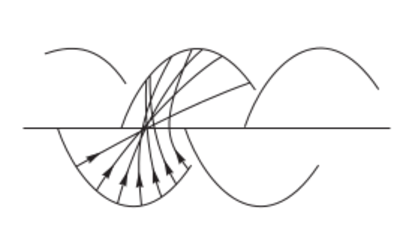
\includegraphics[width=\textwidth]{../../img/testimage.pdf}\caption{testimage}\label{fig:testimage}\end{figure}




\FloatBarrier


L'apparato strumentale consiste di una serie di moduli (amplificatori di alto voltaggio, un fan in/out, un amplificatore analogico, una cassetta dei ritardi, un CFTD e un TAC),
due scintillatori organici di 5 cm, ciascuno collegato a un fotomoltiplicatore XP2020,  un oscilloscopio, un ADC ed un digitizer.
Durante la prima sessione di laboratorio si è preso confidenza con tutte le parti dell'apparato
strumentale e si è fatta la calibrazione di tale apparato. Come prima cosa si sono collegati i rivelatori al fan in/out e il segnale è stato mandato all'oscilloscopio,
in modo che fosse possibile vedere il segnale e misurarne ampiezza, tempo di salita e tempo di discesa. Poi si è ripetuto il procedimento collegando l'amplificatore, e si
sono anche collegati il CFTD e il TAC per la prova della misura di tempo. Una volta capito il funzionamento dei vari moduli, si è proceduto con la regolazione della soglia:
dopo aver collegato tutti i moduli all'oscilloscopio si è visto il segnale del CFTD in concomitanza con il segnale in uscita direttamente dall'amplificatore: in
questo modo è stato possibile verificare che non ci fossero falsi eventi, e regolando un trimmer si è scelta la soglia del CFTD in modo che fosse la più bassa possibile
ma senza registrare falsi eventi a causa del rumore elettronico. Infine si è preso un file di prova per verificare il corretto funzionamento del sistema di misura.\\

Subito dopo si è passati alla vera e propria calibrazione in energia: per prendere i dati si è impostato il sistema di acquisizione in modo che triggherasse singolarmente
sui segnali provenienti dal primo rivelatore e poi su quelli provenienti dal secondo rivelatore. Si sono quindi acquisiti due campioni di dati per una durata di circa 
15 minuti l'uno, che
contenessero entrambe le spalle Compton del decadimento del sodio, da usare per la calibrazione in energia.\\

Durante la seconda sessisone si è passati alla calibrazione in tempo e alla misura del ritardo dei cavi forniti. Per farla, si è triggherato sul segnale di VALID CONV del TAC in modo che venissero registrati solo gli eventi in coincidenza entro 100 ns; andando a modificare i ritardi introdotti si sono poi studiati i grafici risultanti. Dopodichè si sono misurati i ritardi legati ai cavetti aggiungendoli
in serie all'uscita della scatola dei ritardi, acquisendo altri campioni.\\

Successivamente si è passati allo studio della risoluzione temporale in funzione del delay: si è cambiato il cavo del delay utilizzato dal CFTD e si sono studiate le
risoluzioni al variare della lunghezza di tale cavo, in modo da trovare la lunghezza ottimale per la presa dati successiva. Inoltre, collegando una delle uscite del
CFTD assieme al CF MONITOR all'oscilloscopio si è modificato il trimmer WALK ADJ in modo tale che l'intersezione dei segnali bipolari visti sull'oscilloscopio
coincidesse con la baseline del segnale stesso, e che quindi la misura di tempo fosse la migliore possibile.\\

Una volta effettuate tutte le calibrazioni e le regolazioni necessarie si è deciso di prendere una misura che potesse dare una stima della risoluzione temporale al
variare dell'energia, così si è sostituita la sorgente di $^{22}\text{Na}$ con una sorgente di $^{60}\text{Co}$ (che emette fotoni in coincidenza più energetici, sebbene non collineari)
e si è verificato che tutte le regolazioni dell'apparato fossero tali da poter prendere una misura che fosse la migliore possibile. Tale misura è stata presa
nell'intervallo tra la seconda e la terza sessione di laboratorio (è servito un campione più  lungo considerando che i fotoni erano collineari solo come accidente).\\

La terza sessione è stata dedicata alla misura della velocità della luce e all'utilizzo del sistema di acquisizione digitale. Per tale misura,
come prima cosa si è posizionata la sorgente di $^{22}\text{Na}$, che decade attraverso due fotoni collineari, e si è controllato che tutti i parametri della strumentazione
(in particolare i ritardi inseriti nella cassetta, il filo del delay del CFTD, la soglia e il WALF ADJ) fossero quelli ottimali per la presa dati. Dopodiché si sono allontanati
i due rivelatori il più possibile e
si è avvicinata la sorgente al rivelatore 1: triggherando su tale rivelatore si sono osservati i segnali in coincidenza. Si sono in seguito cambiati i valori dell'amplificatore
e della cassetta dei ritardi per fare in modo che i segnali avessero una larghezza di circa 150 ns e fossero distanziati il più possibile. Settato l'apparato, si è presa una
misura di circa un'ora con la sorgente vicina al primo rivelatore e un'altra con la sorgente vicina al secondo rivelatore e si sono misurate le distanze caratteristiche del 
sistema.\\

Come ultima cosa si è passati al sistema di acquisizione digitale: si sono collegati i cavi del sistema (preimpostato) di acquisizione digitale
e si è preso un campione in uscita dai due rivelatori indipendentemente, lungo circa una ventina di minuti.


\FloatBarrier


\section{Analisi Dati}

%\documentclass[a4paper]{article}
%\usepackage[italian]{babel}
%\usepackage[utf8]{inputenc}
%\usepackage{amsmath}
%\usepackage{float}
%\usepackage{multirow}
%\usepackage{multicol}
%\usepackage{graphicx}
%\usepackage{siunitx}
%\usepackage{subcaption}
%\usepackage{verbatim}
%\nonstopmode

%\begin{document}
\subsection{Analisi preliminare dei segnali}

Si riportano i dati ottenuti dall'analisi dei segnali dei rivelatori direttamente sull'oscilloscopio. Il segnale
ottenuto è simile per entrambi i rivelatori, sono infatti entrambi negativi e presentano le seguenti caratteristiche:\\

%\begin{minipage} [B]{0.49\linewidth}
%\large{Segnale Rivelatore 1}
%\( T_{salita} \left(10 \% / 90 \% \right) = (4.4 \pm 0.6) ns \) \\
%\( T_{discesa} \left(10 \% / 90 \% \right)= (11.2 \pm 0.6) ns \) \\
%\( Amp = (1.20 \pm 0.03) V  \) \\
%\end{minipage}
%\rule[-1.2cm]{0.3mm}{3cm}
%\begin{minipage} [B]{0.49\linewidth}
%\large{Segnale Rivelatore 2} 
%\( T_{salita} \left(10 \% / 90 \% \right)= (3.8 \pm 0.3) ns \) \\
%\( T_{discesa} \left(10 \% / 90 \% \right)= (10.8 \pm 0.6) ns \) \\
%\( Amp = (1.16 \pm 0.03) V  \) \\
%\end{minipage}
%\vspace{0.5 cm}
%
\begin{table}[h]
	\centering
	\input{tables/calibrazione_iniziali.tex}
	\caption{Le misure preliminari in uscita dei rivelatori}
	\label{tab:calib_pre}
\end{table}
%

Per misurare i tempi di salita (allontanamento dalla baseline) e di discesa si è misurato il tempo impiegato dal segnale per passare dal 10\% al 90\% dell'ampiezza
massima per la discesa e viceversa per la salita; gli errori sono stati stimati come semplici errori associati alla lettura da oscilloscopio.\\

%A questo punto si è voluto visualizzare  il segnale bipolare dell'amplificatore ORTEC 855, costituito a sua volta da una moltitudine di segnali di ampiezza variabile, proporzionali
%all'energia rilasciata dai fotoni nel rivelatore. I segnali di ampiezza massima (non prendendo in considerazione segnali totalmente fuori scala imputabili ad esempio ad eventuali
%raggi cosmici) sono quelli corrispondenti al Compton Edge del fotone a 1275 KeV. Triggherando con il segnale logico del CFTD di un rivelatore ed osservando l'output bipolare dell'altro,
%si è invece in grado di vedere gli eventi in coincidenza (fotoni emessi back to back) e di conseguenza i segnali ad ampiezza massima corrispondono al Compton Edge del fotone a 511KeV.

\subsection{Calibrazione in Energia}
Gli spettri presi presentano i classici Compton edge relativi ai fotoni a 511KeV e 1275KeV riconducibili rispettivamente
all'annichilazione del positrone prodotto dal decadimento della sorgente di sodio ed un elettrone presente nel materiale ed il decadimento gamma del neon. Le due spalle Compton possono
essere interpolate tramite una gaussiana di cui ci si ricava centroide e sigma. I centroidi non corrispondono però con i Compton edge veri e propri, che valgono
340KeV e 1062KeV per i due fotoni sopracitati: infatti al crescere della sigma si osserva uno shift verso sinistra dei centroidi relativi alle due spalle Compton
per effetto della risoluzione finita dello strumento. \\
Si può però correlare il parametro adimensionale \(\frac{s}{C}\) con il valore in KeV della sigma e quest'ultima al valore dello shift tramite delle funzioni di 
risposta, in maniera tale da poter associare al centroide un valore in energia pari a \(E_{\text{centroide}} = E_{\text{CE}} - E_{\text{shift}}\).  Nelle tabelle
sottostanti si possono leggere i parametri ottenuti interpolando i Compton edge e le conseguenti correzioni del valore in energia dei centroidi\footnote{I grafici
delle interpolazioni si possono vedere nelle \textit{appendici}.}. Poichè questa procedura è stata effettuata a mano non è stato possibile fare una stima degli errori 
associati alle energie dei Compton edge.


%
\begin{table}[h]
	\centering
	\input{tables/calibrazione_shift_1.tex}
	\caption{Procedura calibrazione del rivelatore 1}
	\label{tab:calib_shift_1}
\end{table}
%
%
\begin{table}[h]
	\centering
	\input{tables/calibrazione_shift_2.tex}
	\caption{Procedura calibrazione del rivelatore 2}
	\label{tab:calib__shift_2}
\end{table}
%
Avendo quindi due coppie di valori corrispondeti ai due Compton edge, è possibile ottenere un grafico che permette di calibrare gli spettri in energia.
Essendo i punti a disposizione per ogniuna delle interpolazioni solamente due non si è potuto fornire gli errori relativi ai parametri dell'interpolazione. Inoltre per
trovare i centroidi è stata eseguita la correzione dovuta alla finitezza della risoluzione sopra descritta; dato che questa correzione fa uso di grafici ottenuti
sperimentalmente senza errori, non si è ritenuto opportuna la stima di errori legati ai parametri di calibrazione.


\input{./graphs/calibenergy_r1}
\input{./graphs/calibenergy_r2}

\input{./graphs/spettro_analog}

\section{Calibrazione in Tempo}

A questo punto si è proceduto con la calibrazione in tempo, acquisendo lo spettro del TAC (CH1 canale dell'MCA) avendo settato differenti ritardi tramite 
un'apposita cassetta dei ritardi. Interpolando tali spettri con una gaussiana si è potuto ottenere nuovamente centroide con relativo 
errore corrispondenti ai vari ritardi della delay unit (tra i 4 ns ed i 30 ns) ,
ed effettuando quindi un'interpolazione lineare. Nella seguente tabella si possono vedere i risultati dell'interpolazione gaussiana usati per la calibrazione. Si presenta qui per brevità solo un grafico contenente tutti gli spettri insieme privi di fit (Fig \ref{hist:calib_delay}). \footnote{i singoli grafici di interpolazione gaussiana possono essere visti in Appendice.}. \\

\input{./hist/calib_delay}
%
\begin{table}[h]
	\centering
	\input{tables/calibrazione_delay_unit.tex}
	\caption{Calibrazione della delay unit}
	\label{tab:calib_delay}
\end{table}
%
%
%\begin{tabella}[h]
%	\centering
%	\input{tables/calibrazione_cavi.tex}
%	\caption{Calibrazione cavi}
%	\label{tab:calib_cavi}
%\end{tabella}
%
\input{./graphs/CalibTempo}
%\input{./graphs/CalibCavi}

La dipendenza lineare attesa è stata ben riscontrata.
A seguito di tale calibrazione è stato possibile ricavare il ritardo associato all'inserimento di cavi LEMO tra il Delay e lo stop del TAC ricavando il centroide dai vari spettri del 
TAC ed associandovi un ritardo ricavato tramite i parametri del precedente fit. La relazione lineare che vede in ascissa i tempi ed i relativi centroidi in ordinata è stata 
quindi invertita ricavandosi per propagazione gli errori sui nuovi parametri ed ottenendo i seguenti risultati. Il ritardo associato ai cavetti di diversa lunghezza è molto simile
a quello indicato, la differenza è forse dovuta ad approssimazioni o ad effetti strumentali.\\

\input{./graphs/tempo_cavi}

\begin{table}[h]
	\centering
	\input{tables/extracavi.tex}
	\caption{Stima del ritardo introdotto dai cavi}
	\label{tab:calib_cavi}
\end{table}
 
Infine si è verificato che il delay esterno del CFD che massimizzasse la risoluzione fosse quello di 4ns, ottenuto tramite un apposito cavo LEMO. Si sono confrontati tre diversi cavi
che determinassero un ritardo da 3ns, 4ns e 5ns acquisendo lo spettro del TAC e limitandosi a confrontare solamente le sigma essendo i centroidi sostanzialmente uguali. Ciò che si 
è osservato è che il picco con sigma minore era quello relatvo al ritardo da 4ns, determinando quindi la scelta di usare tale cavo per le misure succesive. Di seguito in tabella
i risultati dei fit gaussiani in canali effettuati sugli spettri\footnote{Come prima, nelle appendici si possono vedere i grafici delle interpolazioni gaussiane.}. \\

\begin{table}[h]
	\centering
	\input{tables/tabellawalkcross.tex}
	\caption{Stima del ritardo introdotto dai cavi}
	\label{tab:calib_walkcross}
\end{table}




\subsection{Velocità della luce}

Si vuole utilizzare l'apparato a disposizione per misurare la velocità della luce. Si noti che con tale apparato è possibile misurare solamente differenze di tempi
e non tempi assoluti (vista tutta l'elettronica utilizzata). Le misure sono state prese come descritto nell'analisi dati, e a disposizione quindi si hanno:
\begin{itemize}
\item la distanza tra i due rivelatori
\item i diversi ritardi nella rivelazione nelle due diverse configurazioni
\item le dimensioni del piombo contenente la sorgente
\item il datasheet dei rivelatori
\end{itemize}
Si cerchi una formula per ricavare la velocità della luce date queste informazioni. Il ragionamento farà uso di due approssimazioni: la sorgente è puntiforme lungo la direzione
di volo dei fotoni rivelati (assumibile in quanto consisteva in un disco posto in maniera perpendicolare a tale direzione)
e si può pensare il fotone venga rivelato sempre nella stessa posizione dentro il rivelatore.\\

Con tali ipotesi, si considerino le misure di lunghezze con la seguente notazione:
\begin{itemize}
\item $R_1$ indica lo spazio medio percorso dai fotoni nel rivelatore prima di interagire con lo stesso
\item $x_1$ indica la distanza tra la placca in piombo più vicina e il rivelatore 1
\item $\delta_1$ indica lo spessore della placca in piombo più vicina al rivelatore 1
\end{itemize}
E analoga notazione per quanto riguarda il rivelatore 2. In poche parole le ipotesi fatte consistono nel fatto che i valori di $R_1$ $R_2$ si possono prendere
come esatti.\footnote{In realtà, questa ipotesi viene verificata nel limite delle infinite misure; dato che il campione preso è sufficientemente grande, si suppone essa sia
valida}, mentre l'ipotesi di sorgente puntiforme è necessaria per ridurre il problema in tre dimensioni a un problema unidimensionale.\\
\input{./img/schema_cobalto}

A questo punto, se la configurazione è la A, si possono descrivere i tempi di percorrenza dei fotoni prima che vengano rivelati come:
$$
  t_{1A} = \frac{\delta_1 + nR_1}{c} \hspace{2cm} t_{2A} = \frac{\delta_2 + x_2 + nR_2}{c}
$$
Ove $n$ indica un eventuale coefficiente di rifrazione all'interno del rivelatore stesso. Quindi il TAC rivelerà l'intervallo temporale:
$$
  \delta t_A = t_{2A} - t_{1A} = \frac{\delta_2 + x_2 + nR_2-\delta_1-nR_1}{c}
$$
Analogamente per la configurazione B si trova:
$$
  t_{1B} = \frac{\delta_1 + x_1 + nR_1}{c} \hspace{2cm} t_{2B} = \frac{\delta_2 + nR_2}{c}
$$
e l'intervallo rilevato dal TAC sarà:
$$
  \Delta t_B = t_{2B} - t_{1B} = \frac{\delta_2 + nR_2 - \delta_1 - x_1 - nR_1}{c}
$$
A questo punto, però, questi due intervalli non hanno senso presi singolarmente, in quanto non rivelano effettivamente un intervallo temporale ma il tempo riferito ad
uno zero che, sebbene non sia noto oggettivamente, è lo stesso per entrambe le misure (infatti non si è toccato l'apparato strumentale se non per spostare la sorgente
racchiusa tra le placche di piombo). Perciò ha senso fisico la loro differenza, che si può stimare con facilità:
$$
  \Delta t = \Delta t_A - \Delta t_B = \frac{{\delta_2 + x_2 + nR_2 - \delta_1 - nR_1}{-\delta_2 - nR_2 + \delta_1 + x_1 + nR_1}}{c} = \frac{x_1 + x_2}{c}
$$
Perciò per stimare la velocità della luce è sufficiente andare a misurare la distanza dei due rivelatori a meno delle placche di piombo e la distanza temporale tra i due
picchi nei grafici calibrati del TAC. Però, in sede di esecuzione dell'esperimento, non si è effettivamente misurata quella distanza ma solamente le distanze tra la sorgente
e i rivelatori nelle due configurazioni, quindi si ha una stima di $\delta$ e una stima di $ 2 \delta + x$ per i due casi.\\

Si venga alla vera e propria analisi dati: si vuole applicare la formula, appena dimostrata:
$$
  c = \frac{x_1+x_2}{\Delta t}
$$
si ragioni sul numeratore, cioè la misura di lunghezza: si conoscono i valori, misurati con il metro:
$$
  d = 173.2 cm \hspace{2cm} \delta = 3.7 cm
$$
ove d indica la distanza tra i due rivelatori e $\delta$ indica le misure (uguali) dei blocchi di piombo.
Ora si è interessati a $x_1+x_2$, per motivi geometrici si può riscrivere in funzione delle variabili misurate come:
$$
  x_1+x_2 = 2 ( d - 2 \delta)
$$
Come errore sulle variabili si considera un errore triangolare associato al fatto che il metro aveva una scala dei millimetri, quindi si ha
$$
  \sigma_d = \sigma_\delta = \frac{0.5\text{mm}}{\sqrt6} = 0.2 mm
$$
\\

Ora si pensi al denominatore dell'equazione per la velocità della luce, cioè la differenza tra le distanze temporali nelle due diverse configurazioni dell'esperimento.
Si riscriva tenendo conto della calibrazione:
$$
  \Delta t = \Delta t_A - \Delta t_B = m\Delta t_A + q - m\Delta t_B - q = m (\Delta t_A - \Delta t_B) 
$$
Ove $m,q$, sono i coefficienti della calibrazione stimati nelle sezioni precedenti. I due picchi si possono vedere, già calibrati, nella figura sottostante.\\
\input{./graphs/light}
Nonostante questa figura sia utile da vedere in quanto calibrata, è necessario operare con i centroidi non calibrati se si vuole avere un'analisi che tenga conto anche
della correlazione degli errori di calibrazione. Quindi, nella tabella sottostante, si riportano i valori dei centroidi sia prima della calibrazione (quindi in canali)
che dopo la calibrazione (e quindi in nanosecondi), con gli errori presentati come errori sui parametri dell'interpolazione fatta:
\input{tables/luce_centroidi}


Presentati questi dati, è possibile passare alla vera e propria stima della velocità della luce, alla quale è ovviamente necessario associare un errore. Dati i preamboli
fatti, si può considerare la formula (espansa in modo da risolvere i problemi di correlazione, perciò è possibile ottenere l'errore tramite semplice propagazione
lineare):
$$
  c = \frac{2 ( d - 2 \delta)}{m (\Delta t_A - \Delta t_B)_\text{canali}} = (2.951 \pm 0.011) \times 10^8 m/s 
$$
\\

Si noti che non si sta considerando correlazione tra le misure spaziali (cioè si considera il metro supponendo che la scala su di esso stampata sia perfetta)


\subsection{Analisi dai dati digitali}
Si è usato il campione preso con il digitizer per fare un confronto tra le misure prese con l'apparato analogico e quelle prese digitalmente.\\
Per prima cosa è stato ricavato un segnale medio per canale, ottenendo così tempo di salita, di discesa e ampiezza media. I due grafici ottenuti sono mostrati in Fig. \ref{gr:mean_signal_0} e Fig. \ref{gr:mean_signal_1}

\input{./graphs/mean_signal_0}
\input{./graphs/mean_signal_1}

Tabella bella

Filtrando dal campione solo gli eventi in coincidenza (presa contando gli eventi il cui time tag differisse meno di 100 ns), si è poi fatta un analisi della risoluzione temporale dell'apparato digitale. Per le misure di tempo si è usato un algoritmo simile al CFTD analogico, facendo variare il ritardo tra i 4 e i 12 ns e l'attenuazione tra lo 0.2 e lo 0.8. Per la ricerca del punto di zero cressing si è fatta un interpolazione con una cubica tra i punti di massimo e minimo del segnale di ``CF monitor'', dato che l'interpolazione suggerita con una retta aveva diversi problemi dovuti alla bassa frequenza di campionamento (vedi Fig. \ref{gr:fail_retta_interp}) che davano una distribuzione temporale distorta.
Le distribuzioni ottenute al variare dei parametri sono state sovrapposte in Fig. \ref{hist:confronto_ris_temp_digi}, mostrando che la risoluzione migliore si ha quando il ritardo è di 4 ns e l'attenuazione è a 0.3. Dato però che questa distribuzione risulta essere leggermente deformata, si è preferito usare l'attenuazione a 0.4, la seconda migliore.

\input{./hist/confronto_ris_temp_CFTD}

tabella risoluzioni gaussiane

Una volta ottimizzato il CFTD, si è proceduto ad analizzare la risoluzione temporale in funzione di una soglia in energia. Fatta una calibrazione dei canali approssimativa sovrapponendo lo spettro totale (privo di coincidenza) con lo spettro ottenuto analogicamente, si è applicato l'algoritmo agli eventi con un energia minore di una di una soglia, variabile tra i 50 e i 350 keV. Le distribuzioni ottenute sono in Fig. \ref{hist:confronto_ris_temp_energy}

\input{./hist/confronto_ris_temp_energy}

tabella risoluzioni gaussiane


\FloatBarrier


\input{sections/chapters/PLACEHOLDER.txt}
\FloatBarrier


	
%appendix

\section{appendice test}
Le appendici invece vanno qua, con la stessa convenzione di numeri che per i capitoli
\begin{tikzpicture}
\pgfdeclareplotmark{cross} {
\pgfpathmoveto{\pgfpoint{-0.3\pgfplotmarksize}{\pgfplotmarksize}}
\pgfpathlineto{\pgfpoint{+0.3\pgfplotmarksize}{\pgfplotmarksize}}
\pgfpathlineto{\pgfpoint{+0.3\pgfplotmarksize}{0.3\pgfplotmarksize}}
\pgfpathlineto{\pgfpoint{+1\pgfplotmarksize}{0.3\pgfplotmarksize}}
\pgfpathlineto{\pgfpoint{+1\pgfplotmarksize}{-0.3\pgfplotmarksize}}
\pgfpathlineto{\pgfpoint{+0.3\pgfplotmarksize}{-0.3\pgfplotmarksize}}
\pgfpathlineto{\pgfpoint{+0.3\pgfplotmarksize}{-1.\pgfplotmarksize}}
\pgfpathlineto{\pgfpoint{-0.3\pgfplotmarksize}{-1.\pgfplotmarksize}}
\pgfpathlineto{\pgfpoint{-0.3\pgfplotmarksize}{-0.3\pgfplotmarksize}}
\pgfpathlineto{\pgfpoint{-1.\pgfplotmarksize}{-0.3\pgfplotmarksize}}
\pgfpathlineto{\pgfpoint{-1.\pgfplotmarksize}{0.3\pgfplotmarksize}}
\pgfpathlineto{\pgfpoint{-0.3\pgfplotmarksize}{0.3\pgfplotmarksize}}
\pgfpathclose
\pgfusepathqstroke
}
\pgfdeclareplotmark{cross*} {
\pgfpathmoveto{\pgfpoint{-0.3\pgfplotmarksize}{\pgfplotmarksize}}
\pgfpathlineto{\pgfpoint{+0.3\pgfplotmarksize}{\pgfplotmarksize}}
\pgfpathlineto{\pgfpoint{+0.3\pgfplotmarksize}{0.3\pgfplotmarksize}}
\pgfpathlineto{\pgfpoint{+1\pgfplotmarksize}{0.3\pgfplotmarksize}}
\pgfpathlineto{\pgfpoint{+1\pgfplotmarksize}{-0.3\pgfplotmarksize}}
\pgfpathlineto{\pgfpoint{+0.3\pgfplotmarksize}{-0.3\pgfplotmarksize}}
\pgfpathlineto{\pgfpoint{+0.3\pgfplotmarksize}{-1.\pgfplotmarksize}}
\pgfpathlineto{\pgfpoint{-0.3\pgfplotmarksize}{-1.\pgfplotmarksize}}
\pgfpathlineto{\pgfpoint{-0.3\pgfplotmarksize}{-0.3\pgfplotmarksize}}
\pgfpathlineto{\pgfpoint{-1.\pgfplotmarksize}{-0.3\pgfplotmarksize}}
\pgfpathlineto{\pgfpoint{-1.\pgfplotmarksize}{0.3\pgfplotmarksize}}
\pgfpathlineto{\pgfpoint{-0.3\pgfplotmarksize}{0.3\pgfplotmarksize}}
\pgfpathclose
\pgfusepathqfillstroke
}
\pgfdeclareplotmark{newstar} {
\pgfpathmoveto{\pgfqpoint{0pt}{\pgfplotmarksize}}
\pgfpathlineto{\pgfqpointpolar{44}{0.5\pgfplotmarksize}}
\pgfpathlineto{\pgfqpointpolar{18}{\pgfplotmarksize}}
\pgfpathlineto{\pgfqpointpolar{-20}{0.5\pgfplotmarksize}}
\pgfpathlineto{\pgfqpointpolar{-54}{\pgfplotmarksize}}
\pgfpathlineto{\pgfqpointpolar{-90}{0.5\pgfplotmarksize}}
\pgfpathlineto{\pgfqpointpolar{234}{\pgfplotmarksize}}
\pgfpathlineto{\pgfqpointpolar{198}{0.5\pgfplotmarksize}}
\pgfpathlineto{\pgfqpointpolar{162}{\pgfplotmarksize}}
\pgfpathlineto{\pgfqpointpolar{134}{0.5\pgfplotmarksize}}
\pgfpathclose
\pgfusepathqstroke
}
\pgfdeclareplotmark{newstar*} {
\pgfpathmoveto{\pgfqpoint{0pt}{\pgfplotmarksize}}
\pgfpathlineto{\pgfqpointpolar{44}{0.5\pgfplotmarksize}}
\pgfpathlineto{\pgfqpointpolar{18}{\pgfplotmarksize}}
\pgfpathlineto{\pgfqpointpolar{-20}{0.5\pgfplotmarksize}}
\pgfpathlineto{\pgfqpointpolar{-54}{\pgfplotmarksize}}
\pgfpathlineto{\pgfqpointpolar{-90}{0.5\pgfplotmarksize}}
\pgfpathlineto{\pgfqpointpolar{234}{\pgfplotmarksize}}
\pgfpathlineto{\pgfqpointpolar{198}{0.5\pgfplotmarksize}}
\pgfpathlineto{\pgfqpointpolar{162}{\pgfplotmarksize}}
\pgfpathlineto{\pgfqpointpolar{134}{0.5\pgfplotmarksize}}
\pgfpathclose
\pgfusepathqfillstroke
}
\definecolor{c}{rgb}{1,1,1};
\draw [color=c, fill=c] (0,0) rectangle (20,13.4957);
\draw [color=c, fill=c] (1.9914,1.37536) rectangle (18.0086,12.149);
\definecolor{c}{rgb}{0,0,0};
\draw [c,line width=0.9] (1.9914,1.37536) -- (1.9914,12.149) -- (18.0086,12.149) -- (18.0086,1.37536) -- (1.9914,1.37536);
\definecolor{c}{rgb}{1,1,1};
\draw [color=c, fill=c] (1.9914,1.37536) rectangle (18.0086,12.149);
\definecolor{c}{rgb}{0,0,0};
\draw [c,line width=0.9] (1.9914,1.37536) -- (1.9914,12.149) -- (18.0086,12.149) -- (18.0086,1.37536) -- (1.9914,1.37536);
\definecolor{c}{rgb}{0,0,0.6};
\draw [c,line width=0.9] (1.9914,10.3292) -- (2.18915,10.3292) -- (2.18915,9.99278) -- (2.38689,9.99278) -- (2.38689,10.3582) -- (2.58463,10.3582) -- (2.58463,10.063) -- (2.78238,10.063) -- (2.78238,10.91) -- (2.98012,10.91) -- (2.98012,10.1186) --
 (3.17786,10.1186) -- (3.17786,11.4327) -- (3.37561,11.4327) -- (3.37561,11.0987) -- (3.57335,11.0987) -- (3.57335,11.2947) -- (3.77109,11.2947) -- (3.77109,10.3122) -- (3.96884,10.3122) -- (3.96884,11.3383) -- (4.16658,11.3383) -- (4.16658,10.7236)
 -- (4.36432,10.7236) -- (4.36432,11.515) -- (4.56206,11.515) -- (4.56206,10.8398) -- (4.75981,10.8398) -- (4.75981,11.4036) -- (4.95755,11.4036) -- (4.95755,10.8374) -- (5.15529,10.8374) -- (5.15529,11.2705) -- (5.35304,11.2705) -- (5.35304,10.8422)
 -- (5.55078,10.8422) -- (5.55078,11.5827) -- (5.74852,11.5827) -- (5.74852,10.8446) -- (5.94627,10.8446) -- (5.94627,11.2972) -- (6.14401,11.2972) -- (6.14401,10.9269) -- (6.34175,10.9269) -- (6.34175,11.3794) -- (6.5395,11.3794) -- (6.5395,10.8567)
 -- (6.73724,10.8567) -- (6.73724,11.3141) -- (6.93498,11.3141) -- (6.93498,10.772) -- (7.13272,10.772) -- (7.13272,11.0915) -- (7.33047,11.0915) -- (7.33047,10.8132) -- (7.52821,10.8132) -- (7.52821,11.636) -- (7.72595,11.636) -- (7.72595,10.7914)
 -- (7.9237,10.7914) -- (7.9237,11.348) -- (8.12144,11.348) -- (8.12144,10.1646) -- (8.31918,10.1646) -- (8.31918,11.1616) -- (8.51693,11.1616) -- (8.51693,10.184) -- (8.71467,10.184) -- (8.71467,11.1907) -- (8.91241,11.1907) -- (8.91241,10.1452) --
 (9.11016,10.1452) -- (9.11016,10.4381) -- (9.3079,10.4381) -- (9.3079,9.85484) -- (9.50564,9.85484) -- (9.50564,10.4865) -- (9.70339,10.4865) -- (9.70339,9.62978) -- (9.90113,9.62978) -- (9.90113,10.2227) -- (10.0989,10.2227) -- (10.0989,9.06833) --
 (10.2966,9.06833) -- (10.2966,9.5112) -- (10.4944,9.5112) -- (10.4944,8.99331) -- (10.6921,8.99331) -- (10.6921,9.19417) -- (10.8898,9.19417) -- (10.8898,8.92313) -- (11.0876,8.92313) -- (11.0876,9.23289) -- (11.2853,9.23289) -- (11.2853,8.10033) --
 (11.4831,8.10033) -- (11.4831,8.49479) -- (11.6808,8.49479) -- (11.6808,8.08581) -- (11.8786,8.08581) -- (11.8786,8.19229) -- (12.0763,8.19229) -- (12.0763,7.93093) -- (12.274,7.93093) -- (12.274,7.38159) -- (12.4718,7.38159) -- (12.4718,7.07182) --
 (12.6695,7.07182) -- (12.6695,7.1783) -- (12.8673,7.1783) -- (12.8673,6.5007) -- (13.065,6.5007) -- (13.065,6.81772) -- (13.2628,6.81772) -- (13.2628,6.3192) -- (13.4605,6.3192) -- (13.4605,6.32646) -- (13.6582,6.32646) -- (13.6582,5.811) --
 (13.856,5.811) -- (13.856,6.04332) -- (14.0537,6.04332) -- (14.0537,5.5085) -- (14.2515,5.5085) -- (14.2515,5.83762) -- (14.4492,5.83762) -- (14.4492,4.82605) -- (14.647,4.82605) -- (14.647,4.50903) -- (14.8447,4.50903) -- (14.8447,4.69295) --
 (15.0424,4.69295) -- (15.0424,4.85993) -- (15.2402,4.85993) -- (15.2402,4.48241) -- (15.4379,4.48241) -- (15.4379,4.30091) -- (15.6357,4.30091) -- (15.6357,3.61847) -- (15.8334,3.61847) -- (15.8334,3.88467) -- (16.0312,3.88467) -- (16.0312,3.40793)
 -- (16.2289,3.40793) -- (16.2289,3.67171) -- (16.4267,3.67171) -- (16.4267,3.23853) -- (16.6244,3.23853) -- (16.6244,3.09332) -- (16.8221,3.09332) -- (16.8221,2.72064) -- (17.0199,2.72064) -- (17.0199,2.88762) -- (17.2176,2.88762) --
 (17.2176,2.3044) -- (17.4154,2.3044) -- (17.4154,2.41088) -- (17.6131,2.41088) -- (17.6131,1.86396) -- (17.8109,1.86396) -- (17.8109,2.0987) -- (18.0086,2.0987);
\definecolor{c}{rgb}{1,1,1};
\draw [color=c, fill=c] (13.9828,7.30659) rectangle (19.5989,12.6361);
\definecolor{c}{rgb}{0,0,0};
\draw [c,line width=0.9] (13.9828,7.30659) -- (19.5989,7.30659);
\draw [c,line width=0.9] (19.5989,7.30659) -- (19.5989,12.6361);
\draw [c,line width=0.9] (19.5989,12.6361) -- (13.9828,12.6361);
\draw [c,line width=0.9] (13.9828,12.6361) -- (13.9828,7.30659);
\draw [anchor= west] (14.2636,11.9699) node[scale=1.20912, color=c, rotate=0]{Entries };
\draw [anchor= east] (19.3181,11.9699) node[scale=1.20912, color=c, rotate=0]{ 2110265};
\draw [anchor= west] (14.2636,10.6375) node[scale=1.20912, color=c, rotate=0]{Constant };
\draw [anchor= east] (19.3181,10.6375) node[scale=1.20912, color=c, rotate=0]{$  7064 \pm 13.2$};
\draw [anchor= west] (14.2636,9.30516) node[scale=1.20912, color=c, rotate=0]{Mean     };
\draw [anchor= east] (19.3181,9.30516) node[scale=1.20912, color=c, rotate=0]{$ 239.7 \pm 0.3$};
\draw [anchor= west] (14.2636,7.97278) node[scale=1.20912, color=c, rotate=0]{Sigma    };
\draw [anchor= east] (19.3181,7.97278) node[scale=1.20912, color=c, rotate=0]{$ 48.41 \pm 0.36$};
\definecolor{c}{rgb}{1,0,0};
\draw [c,line width=1.8] (2.07149,10.0938) -- (2.23166,10.1924) -- (2.39183,10.2871) -- (2.55201,10.3779) -- (2.71218,10.4646) -- (2.87235,10.5471) -- (3.03252,10.6255) -- (3.19269,10.6997) -- (3.35287,10.7695) -- (3.51304,10.8349) --
 (3.67321,10.896) -- (3.83338,10.9525) -- (3.99355,11.0046) -- (4.15373,11.052) -- (4.3139,11.0949) -- (4.47407,11.1331) -- (4.63424,11.1667) -- (4.79441,11.1955) -- (4.95458,11.2197) -- (5.11476,11.2391) -- (5.27493,11.2537) -- (5.4351,11.2635) --
 (5.59527,11.2686) -- (5.75544,11.2689) -- (5.91562,11.2644) -- (6.07579,11.2551) -- (6.23596,11.2411) -- (6.39613,11.2223) -- (6.5563,11.1987) -- (6.71648,11.1704) -- (6.87665,11.1374) -- (7.03682,11.0998) -- (7.19699,11.0575) -- (7.35716,11.0105)
 -- (7.51734,10.9591) -- (7.67751,10.903) -- (7.83768,10.8425) -- (7.99785,10.7776) -- (8.15802,10.7083) -- (8.31819,10.6347) -- (8.47837,10.5568) -- (8.63854,10.4747) -- (8.79871,10.3885) -- (8.95888,10.2983) -- (9.11905,10.204) -- (9.27923,10.1059)
 -- (9.4394,10.0039) -- (9.59957,9.89814) -- (9.75974,9.78874) -- (9.91991,9.67575);
\draw [c,line width=1.8] (9.91991,9.67575) -- (10.0801,9.55928) -- (10.2403,9.4394) -- (10.4004,9.31623) -- (10.5606,9.18983) -- (10.7208,9.06033) -- (10.8809,8.92781) -- (11.0411,8.79238) -- (11.2013,8.65414) -- (11.3615,8.51319) --
 (11.5216,8.36964) -- (11.6818,8.22359) -- (11.842,8.07516) -- (12.0021,7.92444) -- (12.1623,7.77154) -- (12.3225,7.61659) -- (12.4827,7.45968) -- (12.6428,7.30092) -- (12.803,7.14044) -- (12.9632,6.97833) -- (13.1234,6.8147) -- (13.2835,6.64968) --
 (13.4437,6.48336) -- (13.6039,6.31587) -- (13.764,6.1473) -- (13.9242,5.97776) -- (14.0844,5.80737) -- (14.2446,5.63623) -- (14.4047,5.46444) -- (14.5649,5.29212) -- (14.7251,5.11936) -- (14.8852,4.94628) -- (15.0454,4.77296) -- (15.2056,4.59951) --
 (15.3658,4.42603) -- (15.5259,4.25262) -- (15.6861,4.07936) -- (15.8463,3.90636) -- (16.0064,3.73371) -- (16.1666,3.56149) -- (16.3268,3.38979) -- (16.487,3.21871) -- (16.6471,3.04831) -- (16.8073,2.87869) -- (16.9675,2.70992) -- (17.1277,2.54208)
 -- (17.2878,2.37524) -- (17.448,2.20949) -- (17.6082,2.04488) -- (17.7683,1.88148);
\draw [c,line width=1.8] (17.7683,1.88148) -- (17.9285,1.71937);
\definecolor{c}{rgb}{0,0,0};
\draw [c,line width=0.9] (1.9914,1.37536) -- (18.0086,1.37536);
\draw [anchor= east] (18.0086,0.619599) node[scale=1.01821, color=c, rotate=0]{Canali};
\draw [c,line width=0.9] (3.77109,1.6996) -- (3.77109,1.37536);
\draw [c,line width=0.9] (4.16658,1.53748) -- (4.16658,1.37536);
\draw [c,line width=0.9] (4.56206,1.53748) -- (4.56206,1.37536);
\draw [c,line width=0.9] (4.95755,1.53748) -- (4.95755,1.37536);
\draw [c,line width=0.9] (5.35304,1.53748) -- (5.35304,1.37536);
\draw [c,line width=0.9] (5.74852,1.6996) -- (5.74852,1.37536);
\draw [c,line width=0.9] (6.14401,1.53748) -- (6.14401,1.37536);
\draw [c,line width=0.9] (6.5395,1.53748) -- (6.5395,1.37536);
\draw [c,line width=0.9] (6.93498,1.53748) -- (6.93498,1.37536);
\draw [c,line width=0.9] (7.33047,1.53748) -- (7.33047,1.37536);
\draw [c,line width=0.9] (7.72595,1.6996) -- (7.72595,1.37536);
\draw [c,line width=0.9] (8.12144,1.53748) -- (8.12144,1.37536);
\draw [c,line width=0.9] (8.51693,1.53748) -- (8.51693,1.37536);
\draw [c,line width=0.9] (8.91241,1.53748) -- (8.91241,1.37536);
\draw [c,line width=0.9] (9.3079,1.53748) -- (9.3079,1.37536);
\draw [c,line width=0.9] (9.70339,1.6996) -- (9.70339,1.37536);
\draw [c,line width=0.9] (10.0989,1.53748) -- (10.0989,1.37536);
\draw [c,line width=0.9] (10.4944,1.53748) -- (10.4944,1.37536);
\draw [c,line width=0.9] (10.8898,1.53748) -- (10.8898,1.37536);
\draw [c,line width=0.9] (11.2853,1.53748) -- (11.2853,1.37536);
\draw [c,line width=0.9] (11.6808,1.6996) -- (11.6808,1.37536);
\draw [c,line width=0.9] (12.0763,1.53748) -- (12.0763,1.37536);
\draw [c,line width=0.9] (12.4718,1.53748) -- (12.4718,1.37536);
\draw [c,line width=0.9] (12.8673,1.53748) -- (12.8673,1.37536);
\draw [c,line width=0.9] (13.2628,1.53748) -- (13.2628,1.37536);
\draw [c,line width=0.9] (13.6582,1.6996) -- (13.6582,1.37536);
\draw [c,line width=0.9] (14.0537,1.53748) -- (14.0537,1.37536);
\draw [c,line width=0.9] (14.4492,1.53748) -- (14.4492,1.37536);
\draw [c,line width=0.9] (14.8447,1.53748) -- (14.8447,1.37536);
\draw [c,line width=0.9] (15.2402,1.53748) -- (15.2402,1.37536);
\draw [c,line width=0.9] (15.6357,1.6996) -- (15.6357,1.37536);
\draw [c,line width=0.9] (16.0312,1.53748) -- (16.0312,1.37536);
\draw [c,line width=0.9] (16.4267,1.53748) -- (16.4267,1.37536);
\draw [c,line width=0.9] (16.8221,1.53748) -- (16.8221,1.37536);
\draw [c,line width=0.9] (17.2176,1.53748) -- (17.2176,1.37536);
\draw [c,line width=0.9] (17.6131,1.6996) -- (17.6131,1.37536);
\draw [c,line width=0.9] (3.77109,1.6996) -- (3.77109,1.37536);
\draw [c,line width=0.9] (3.37561,1.53748) -- (3.37561,1.37536);
\draw [c,line width=0.9] (2.98012,1.53748) -- (2.98012,1.37536);
\draw [c,line width=0.9] (2.58463,1.53748) -- (2.58463,1.37536);
\draw [c,line width=0.9] (2.18915,1.53748) -- (2.18915,1.37536);
\draw [c,line width=0.9] (17.6131,1.6996) -- (17.6131,1.37536);
\draw [c,line width=0.9] (18.0086,1.53748) -- (18.0086,1.37536);
\draw [anchor=base] (3.77109,0.93) node[scale=1.01821, color=c, rotate=0]{230};
\draw [anchor=base] (5.74852,0.93) node[scale=1.01821, color=c, rotate=0]{240};
\draw [anchor=base] (7.72595,0.93) node[scale=1.01821, color=c, rotate=0]{250};
\draw [anchor=base] (9.70339,0.93) node[scale=1.01821, color=c, rotate=0]{260};
\draw [anchor=base] (11.6808,0.93) node[scale=1.01821, color=c, rotate=0]{270};
\draw [anchor=base] (13.6582,0.93) node[scale=1.01821, color=c, rotate=0]{280};
\draw [anchor=base] (15.6357,0.93) node[scale=1.01821, color=c, rotate=0]{290};
\draw [anchor=base] (17.6131,0.93) node[scale=1.01821, color=c, rotate=0]{300};
\draw [c,line width=0.9] (1.9914,1.37536) -- (1.9914,12.149);
\draw [anchor= east] (0.871404,12.149) node[scale=1.01821, color=c, rotate=90]{Eventi};
\draw [c,line width=0.9] (2.47038,1.43562) -- (1.9914,1.43562);
\draw [c,line width=0.9] (2.23089,1.67762) -- (1.9914,1.67762);
\draw [c,line width=0.9] (2.23089,1.91962) -- (1.9914,1.91962);
\draw [c,line width=0.9] (2.23089,2.16162) -- (1.9914,2.16162);
\draw [c,line width=0.9] (2.23089,2.40362) -- (1.9914,2.40362);
\draw [c,line width=0.9] (2.47038,2.64562) -- (1.9914,2.64562);
\draw [c,line width=0.9] (2.23089,2.88762) -- (1.9914,2.88762);
\draw [c,line width=0.9] (2.23089,3.12962) -- (1.9914,3.12962);
\draw [c,line width=0.9] (2.23089,3.37163) -- (1.9914,3.37163);
\draw [c,line width=0.9] (2.23089,3.61363) -- (1.9914,3.61363);
\draw [c,line width=0.9] (2.47038,3.85563) -- (1.9914,3.85563);
\draw [c,line width=0.9] (2.23089,4.09763) -- (1.9914,4.09763);
\draw [c,line width=0.9] (2.23089,4.33963) -- (1.9914,4.33963);
\draw [c,line width=0.9] (2.23089,4.58163) -- (1.9914,4.58163);
\draw [c,line width=0.9] (2.23089,4.82363) -- (1.9914,4.82363);
\draw [c,line width=0.9] (2.47038,5.06563) -- (1.9914,5.06563);
\draw [c,line width=0.9] (2.23089,5.30764) -- (1.9914,5.30764);
\draw [c,line width=0.9] (2.23089,5.54964) -- (1.9914,5.54964);
\draw [c,line width=0.9] (2.23089,5.79164) -- (1.9914,5.79164);
\draw [c,line width=0.9] (2.23089,6.03364) -- (1.9914,6.03364);
\draw [c,line width=0.9] (2.47038,6.27564) -- (1.9914,6.27564);
\draw [c,line width=0.9] (2.23089,6.51764) -- (1.9914,6.51764);
\draw [c,line width=0.9] (2.23089,6.75964) -- (1.9914,6.75964);
\draw [c,line width=0.9] (2.23089,7.00164) -- (1.9914,7.00164);
\draw [c,line width=0.9] (2.23089,7.24365) -- (1.9914,7.24365);
\draw [c,line width=0.9] (2.47038,7.48565) -- (1.9914,7.48565);
\draw [c,line width=0.9] (2.23089,7.72765) -- (1.9914,7.72765);
\draw [c,line width=0.9] (2.23089,7.96965) -- (1.9914,7.96965);
\draw [c,line width=0.9] (2.23089,8.21165) -- (1.9914,8.21165);
\draw [c,line width=0.9] (2.23089,8.45365) -- (1.9914,8.45365);
\draw [c,line width=0.9] (2.47038,8.69565) -- (1.9914,8.69565);
\draw [c,line width=0.9] (2.23089,8.93765) -- (1.9914,8.93765);
\draw [c,line width=0.9] (2.23089,9.17965) -- (1.9914,9.17965);
\draw [c,line width=0.9] (2.23089,9.42166) -- (1.9914,9.42166);
\draw [c,line width=0.9] (2.23089,9.66366) -- (1.9914,9.66366);
\draw [c,line width=0.9] (2.47038,9.90566) -- (1.9914,9.90566);
\draw [c,line width=0.9] (2.23089,10.1477) -- (1.9914,10.1477);
\draw [c,line width=0.9] (2.23089,10.3897) -- (1.9914,10.3897);
\draw [c,line width=0.9] (2.23089,10.6317) -- (1.9914,10.6317);
\draw [c,line width=0.9] (2.23089,10.8737) -- (1.9914,10.8737);
\draw [c,line width=0.9] (2.47038,11.1157) -- (1.9914,11.1157);
\draw [c,line width=0.9] (2.47038,1.43562) -- (1.9914,1.43562);
\draw [c,line width=0.9] (2.47038,11.1157) -- (1.9914,11.1157);
\draw [c,line width=0.9] (2.23089,11.3577) -- (1.9914,11.3577);
\draw [c,line width=0.9] (2.23089,11.5997) -- (1.9914,11.5997);
\draw [c,line width=0.9] (2.23089,11.8417) -- (1.9914,11.8417);
\draw [c,line width=0.9] (2.23089,12.0837) -- (1.9914,12.0837);
\draw [anchor= east] (1.8914,1.43562) node[scale=1.01821, color=c, rotate=0]{3000};
\draw [anchor= east] (1.8914,2.64562) node[scale=1.01821, color=c, rotate=0]{3500};
\draw [anchor= east] (1.8914,3.85563) node[scale=1.01821, color=c, rotate=0]{4000};
\draw [anchor= east] (1.8914,5.06563) node[scale=1.01821, color=c, rotate=0]{4500};
\draw [anchor= east] (1.8914,6.27564) node[scale=1.01821, color=c, rotate=0]{5000};
\draw [anchor= east] (1.8914,7.48565) node[scale=1.01821, color=c, rotate=0]{5500};
\draw [anchor= east] (1.8914,8.69565) node[scale=1.01821, color=c, rotate=0]{6000};
\draw [anchor= east] (1.8914,9.90566) node[scale=1.01821, color=c, rotate=0]{6500};
\draw [anchor= east] (1.8914,11.1157) node[scale=1.01821, color=c, rotate=0]{7000};
\definecolor{c}{rgb}{1,1,1};
\draw [color=c, fill=c] (13.9828,7.30659) rectangle (19.5989,12.6361);
\definecolor{c}{rgb}{0,0,0};
\draw [c,line width=0.9] (13.9828,7.30659) -- (19.5989,7.30659);
\draw [c,line width=0.9] (19.5989,7.30659) -- (19.5989,12.6361);
\draw [c,line width=0.9] (19.5989,12.6361) -- (13.9828,12.6361);
\draw [c,line width=0.9] (13.9828,12.6361) -- (13.9828,7.30659);
\draw [anchor= west] (14.2636,11.9699) node[scale=1.20912, color=c, rotate=0]{Entries };
\draw [anchor= east] (19.3181,11.9699) node[scale=1.20912, color=c, rotate=0]{ 2110265};
\draw [anchor= west] (14.2636,10.6375) node[scale=1.20912, color=c, rotate=0]{Constant };
\draw [anchor= east] (19.3181,10.6375) node[scale=1.20912, color=c, rotate=0]{$  7064 \pm 13.2$};
\draw [anchor= west] (14.2636,9.30516) node[scale=1.20912, color=c, rotate=0]{Mean     };
\draw [anchor= east] (19.3181,9.30516) node[scale=1.20912, color=c, rotate=0]{$ 239.7 \pm 0.3$};
\draw [anchor= west] (14.2636,7.97278) node[scale=1.20912, color=c, rotate=0]{Sigma    };
\draw [anchor= east] (19.3181,7.97278) node[scale=1.20912, color=c, rotate=0]{$ 48.41 \pm 0.36$};
\draw (9.24069,12.808) node[scale=1.40004, color=c, rotate=0]{Rivelatore 1, Fotone 511 KeV};
\end{tikzpicture}

\begin{tikzpicture}
\pgfdeclareplotmark{cross} {
\pgfpathmoveto{\pgfpoint{-0.3\pgfplotmarksize}{\pgfplotmarksize}}
\pgfpathlineto{\pgfpoint{+0.3\pgfplotmarksize}{\pgfplotmarksize}}
\pgfpathlineto{\pgfpoint{+0.3\pgfplotmarksize}{0.3\pgfplotmarksize}}
\pgfpathlineto{\pgfpoint{+1\pgfplotmarksize}{0.3\pgfplotmarksize}}
\pgfpathlineto{\pgfpoint{+1\pgfplotmarksize}{-0.3\pgfplotmarksize}}
\pgfpathlineto{\pgfpoint{+0.3\pgfplotmarksize}{-0.3\pgfplotmarksize}}
\pgfpathlineto{\pgfpoint{+0.3\pgfplotmarksize}{-1.\pgfplotmarksize}}
\pgfpathlineto{\pgfpoint{-0.3\pgfplotmarksize}{-1.\pgfplotmarksize}}
\pgfpathlineto{\pgfpoint{-0.3\pgfplotmarksize}{-0.3\pgfplotmarksize}}
\pgfpathlineto{\pgfpoint{-1.\pgfplotmarksize}{-0.3\pgfplotmarksize}}
\pgfpathlineto{\pgfpoint{-1.\pgfplotmarksize}{0.3\pgfplotmarksize}}
\pgfpathlineto{\pgfpoint{-0.3\pgfplotmarksize}{0.3\pgfplotmarksize}}
\pgfpathclose
\pgfusepathqstroke
}
\pgfdeclareplotmark{cross*} {
\pgfpathmoveto{\pgfpoint{-0.3\pgfplotmarksize}{\pgfplotmarksize}}
\pgfpathlineto{\pgfpoint{+0.3\pgfplotmarksize}{\pgfplotmarksize}}
\pgfpathlineto{\pgfpoint{+0.3\pgfplotmarksize}{0.3\pgfplotmarksize}}
\pgfpathlineto{\pgfpoint{+1\pgfplotmarksize}{0.3\pgfplotmarksize}}
\pgfpathlineto{\pgfpoint{+1\pgfplotmarksize}{-0.3\pgfplotmarksize}}
\pgfpathlineto{\pgfpoint{+0.3\pgfplotmarksize}{-0.3\pgfplotmarksize}}
\pgfpathlineto{\pgfpoint{+0.3\pgfplotmarksize}{-1.\pgfplotmarksize}}
\pgfpathlineto{\pgfpoint{-0.3\pgfplotmarksize}{-1.\pgfplotmarksize}}
\pgfpathlineto{\pgfpoint{-0.3\pgfplotmarksize}{-0.3\pgfplotmarksize}}
\pgfpathlineto{\pgfpoint{-1.\pgfplotmarksize}{-0.3\pgfplotmarksize}}
\pgfpathlineto{\pgfpoint{-1.\pgfplotmarksize}{0.3\pgfplotmarksize}}
\pgfpathlineto{\pgfpoint{-0.3\pgfplotmarksize}{0.3\pgfplotmarksize}}
\pgfpathclose
\pgfusepathqfillstroke
}
\pgfdeclareplotmark{newstar} {
\pgfpathmoveto{\pgfqpoint{0pt}{\pgfplotmarksize}}
\pgfpathlineto{\pgfqpointpolar{44}{0.5\pgfplotmarksize}}
\pgfpathlineto{\pgfqpointpolar{18}{\pgfplotmarksize}}
\pgfpathlineto{\pgfqpointpolar{-20}{0.5\pgfplotmarksize}}
\pgfpathlineto{\pgfqpointpolar{-54}{\pgfplotmarksize}}
\pgfpathlineto{\pgfqpointpolar{-90}{0.5\pgfplotmarksize}}
\pgfpathlineto{\pgfqpointpolar{234}{\pgfplotmarksize}}
\pgfpathlineto{\pgfqpointpolar{198}{0.5\pgfplotmarksize}}
\pgfpathlineto{\pgfqpointpolar{162}{\pgfplotmarksize}}
\pgfpathlineto{\pgfqpointpolar{134}{0.5\pgfplotmarksize}}
\pgfpathclose
\pgfusepathqstroke
}
\pgfdeclareplotmark{newstar*} {
\pgfpathmoveto{\pgfqpoint{0pt}{\pgfplotmarksize}}
\pgfpathlineto{\pgfqpointpolar{44}{0.5\pgfplotmarksize}}
\pgfpathlineto{\pgfqpointpolar{18}{\pgfplotmarksize}}
\pgfpathlineto{\pgfqpointpolar{-20}{0.5\pgfplotmarksize}}
\pgfpathlineto{\pgfqpointpolar{-54}{\pgfplotmarksize}}
\pgfpathlineto{\pgfqpointpolar{-90}{0.5\pgfplotmarksize}}
\pgfpathlineto{\pgfqpointpolar{234}{\pgfplotmarksize}}
\pgfpathlineto{\pgfqpointpolar{198}{0.5\pgfplotmarksize}}
\pgfpathlineto{\pgfqpointpolar{162}{\pgfplotmarksize}}
\pgfpathlineto{\pgfqpointpolar{134}{0.5\pgfplotmarksize}}
\pgfpathclose
\pgfusepathqfillstroke
}
\definecolor{c}{rgb}{1,1,1};
\draw [color=c, fill=c] (0,0) rectangle (20,13.4957);
\draw [color=c, fill=c] (1.9914,1.37536) rectangle (18.0086,12.149);
\definecolor{c}{rgb}{0,0,0};
\draw [c,line width=0.9] (1.9914,1.37536) -- (1.9914,12.149) -- (18.0086,12.149) -- (18.0086,1.37536) -- (1.9914,1.37536);
\definecolor{c}{rgb}{1,1,1};
\draw [color=c, fill=c] (1.9914,1.37536) rectangle (18.0086,12.149);
\definecolor{c}{rgb}{0,0,0};
\draw [c,line width=0.9] (1.9914,1.37536) -- (1.9914,12.149) -- (18.0086,12.149) -- (18.0086,1.37536) -- (1.9914,1.37536);
\definecolor{c}{rgb}{0,0,0.6};
\draw [c,line width=0.9] (1.9914,9.71033) -- (2.07189,9.71033) -- (2.07189,10.3575) -- (2.15238,10.3575) -- (2.15238,9.76626) -- (2.23287,9.76626) -- (2.23287,10.5014) -- (2.31336,10.5014) -- (2.31336,9.7343) -- (2.39385,9.7343) -- (2.39385,10.1738)
 -- (2.47433,10.1738) -- (2.47433,10.3336) -- (2.55482,10.3336) -- (2.55482,9.98999) -- (2.63531,9.98999) -- (2.63531,10.1098) -- (2.7158,10.1098) -- (2.7158,10.3655) -- (2.79629,10.3655) -- (2.79629,9.98999) -- (2.87678,9.98999) -- (2.87678,10.3575)
 -- (2.95726,10.3575) -- (2.95726,10.2856) -- (3.03775,10.2856) -- (3.03775,10.3096) -- (3.11824,10.3096) -- (3.11824,9.91807) -- (3.19873,9.91807) -- (3.19873,10.7331) -- (3.27922,10.7331) -- (3.27922,10.5733) -- (3.35971,10.5733) --
 (3.35971,10.9408) -- (3.4402,10.9408) -- (3.4402,10.3895) -- (3.52068,10.3895) -- (3.52068,10.8449) -- (3.60117,10.8449) -- (3.60117,10.2057) -- (3.68166,10.2057) -- (3.68166,10.5493) -- (3.76215,10.5493) -- (3.76215,10.8849) -- (3.84264,10.8849) --
 (3.84264,11.3403) -- (3.92313,11.3403) -- (3.92313,10.4694) -- (4.00361,10.4694) -- (4.00361,10.9888) -- (4.0841,10.9888) -- (4.0841,10.2057) -- (4.16459,10.2057) -- (4.16459,10.773) -- (4.24508,10.773) -- (4.24508,10.5093) -- (4.32557,10.5093) --
 (4.32557,11.3403) -- (4.40606,11.3403) -- (4.40606,10.3815) -- (4.48654,10.3815) -- (4.48654,10.8769) -- (4.56703,10.8769) -- (4.56703,10.4374) -- (4.64752,10.4374) -- (4.64752,10.1658) -- (4.72801,10.1658) -- (4.72801,10.5253) -- (4.8085,10.5253)
 -- (4.8085,11.5081) -- (4.88899,11.5081) -- (4.88899,10.9888) -- (4.96947,10.9888) -- (4.96947,11.5641) -- (5.04996,11.5641) -- (5.04996,10.4694) -- (5.13045,10.4694) -- (5.13045,11.5641) -- (5.21094,11.5641) -- (5.21094,10.6212) --
 (5.29143,10.6212) -- (5.29143,11.1486) -- (5.37192,11.1486) -- (5.37192,10.2137) -- (5.45241,10.2137) -- (5.45241,10.9168) -- (5.53289,10.9168) -- (5.53289,11.0846) -- (5.61338,11.0846) -- (5.61338,11.636) -- (5.69387,11.636) -- (5.69387,10.765) --
 (5.77436,10.765) -- (5.77436,11.3883) -- (5.85485,11.3883) -- (5.85485,10.2297) -- (5.93534,10.2297) -- (5.93534,10.8929) -- (6.01582,10.8929) -- (6.01582,10.4135) -- (6.09631,10.4135) -- (6.09631,11.58) -- (6.1768,11.58) -- (6.1768,10.789) --
 (6.25729,10.789) -- (6.25729,10.8689) -- (6.33778,10.8689) -- (6.33778,10.3735) -- (6.41827,10.3735) -- (6.41827,10.8689) -- (6.49875,10.8689) -- (6.49875,10.6212) -- (6.57924,10.6212) -- (6.57924,10.9248) -- (6.65973,10.9248) -- (6.65973,10.3575)
 -- (6.74022,10.3575) -- (6.74022,10.829) -- (6.82071,10.829) -- (6.82071,10.5253) -- (6.9012,10.5253) -- (6.9012,10.7331) -- (6.98169,10.7331) -- (6.98169,10.7491) -- (7.06217,10.7491) -- (7.06217,10.813) -- (7.14266,10.813) -- (7.14266,10.1258) --
 (7.22315,10.1258) -- (7.22315,10.6372) -- (7.30364,10.6372) -- (7.30364,10.2377) -- (7.38413,10.2377) -- (7.38413,10.9408) -- (7.46462,10.9408) -- (7.46462,10.4055) -- (7.5451,10.4055) -- (7.5451,10.2696) -- (7.62559,10.2696) -- (7.62559,10.2856) --
 (7.70608,10.2856) -- (7.70608,10.5014) -- (7.78657,10.5014) -- (7.78657,10.1498) -- (7.86706,10.1498) -- (7.86706,10.2776) -- (7.94755,10.2776) -- (7.94755,9.69435) -- (8.02803,9.69435) -- (8.02803,9.7343) -- (8.10852,9.7343) -- (8.10852,9.62244) --
 (8.18901,9.62244) -- (8.18901,10.5813) -- (8.2695,10.5813) -- (8.2695,9.23092) -- (8.34999,9.23092) -- (8.34999,10.006) -- (8.43048,10.006) -- (8.43048,9.84616) -- (8.51096,9.84616) -- (8.51096,9.66239) -- (8.59145,9.66239) -- (8.59145,9.84616) --
 (8.67194,9.84616) -- (8.67194,9.49459) -- (8.75243,9.49459) -- (8.75243,9.28685) -- (8.83292,9.28685) -- (8.83292,10.0779) -- (8.91341,10.0779) -- (8.91341,9.35876) -- (8.99389,9.35876) -- (8.99389,9.2469) -- (9.07438,9.2469) -- (9.07438,9.18298) --
 (9.15487,9.18298) -- (9.15487,9.03116) -- (9.23536,9.03116) -- (9.23536,8.50381) -- (9.31585,8.50381) -- (9.31585,9.20695) -- (9.39634,9.20695) -- (9.39634,8.90332) -- (9.47683,8.90332) -- (9.47683,9.0791) -- (9.55731,9.0791) -- (9.55731,8.88734) --
 (9.6378,8.88734) -- (9.6378,9.02317) -- (9.71829,9.02317) -- (9.71829,8.33602) -- (9.79878,8.33602) -- (9.79878,8.43989) -- (9.87927,8.43989) -- (9.87927,7.64886) -- (9.95976,7.64886) -- (9.95976,8.27209) -- (10.0402,8.27209) -- (10.0402,8.24812) --
 (10.1207,8.24812) -- (10.1207,7.81665) -- (10.2012,7.81665) -- (10.2012,7.62489) -- (10.2817,7.62489) -- (10.2817,8.08033) -- (10.3622,8.08033) -- (10.3622,7.86459) -- (10.4427,7.86459) -- (10.4427,7.92852) -- (10.5232,7.92852) -- (10.5232,7.42513)
 -- (10.6037,7.42513) -- (10.6037,7.20141) -- (10.6842,7.20141) -- (10.6842,7.33724) -- (10.7646,7.33724) -- (10.7646,7.36121) -- (10.8451,7.36121) -- (10.8451,7.24136) -- (10.9256,7.24136) -- (10.9256,7.10553) -- (11.0061,7.10553) --
 (11.0061,6.91376) -- (11.0866,6.91376) -- (11.0866,7.07357) -- (11.1671,7.07357) -- (11.1671,6.70602) -- (11.2476,6.70602) -- (11.2476,6.29852) -- (11.3281,6.29852) -- (11.3281,6.5542) -- (11.4085,6.5542) -- (11.4085,6.67406) -- (11.489,6.67406) --
 (11.489,6.46631) -- (11.5695,6.46631) -- (11.5695,6.60214) -- (11.65,6.60214) -- (11.65,6.32249) -- (11.7305,6.32249) -- (11.7305,6.49028) -- (11.811,6.49028) -- (11.811,5.93097) -- (11.8915,5.93097) -- (11.8915,6.2266) -- (11.972,6.2266) --
 (11.972,6.17067) -- (12.0525,6.17067) -- (12.0525,5.93097) -- (12.1329,5.93097) -- (12.1329,5.99489) -- (12.2134,5.99489) -- (12.2134,6.09876) -- (12.2939,6.09876) -- (12.2939,5.4995) -- (12.3744,5.4995) -- (12.3744,6.02685) -- (12.4549,6.02685) --
 (12.4549,5.56342) -- (12.5354,5.56342) -- (12.5354,5.8191) -- (12.6159,5.8191) -- (12.6159,5.22783) -- (12.6964,5.22783) -- (12.6964,5.54744) -- (12.7768,5.54744) -- (12.7768,5.3317) -- (12.8573,5.3317) -- (12.8573,5.43558) -- (12.9378,5.43558) --
 (12.9378,4.94018) -- (13.0183,4.94018) -- (13.0183,5.19587) -- (13.0988,5.19587) -- (13.0988,4.67651) -- (13.1793,4.67651) -- (13.1793,5.10798) -- (13.2598,5.10798) -- (13.2598,4.69249) -- (13.3403,4.69249) -- (13.3403,4.54866) -- (13.4208,4.54866)
 -- (13.4208,4.71646) -- (13.5012,4.71646) -- (13.5012,4.78038) -- (13.5817,4.78038) -- (13.5817,4.49273) -- (13.6622,4.49273) -- (13.6622,4.67651) -- (13.7427,4.67651) -- (13.7427,4.22107) -- (13.8232,4.22107) -- (13.8232,4.40484) --
 (13.9037,4.40484) -- (13.9037,4.49273) -- (13.9842,4.49273) -- (13.9842,4.26901) -- (14.0647,4.26901) -- (14.0647,4.13317) -- (14.1452,4.13317) -- (14.1452,4.24504) -- (14.2256,4.24504) -- (14.2256,4.07724) -- (14.3061,4.07724) -- (14.3061,3.98136)
 -- (14.3866,3.98136) -- (14.3866,3.97337) -- (14.4671,3.97337) -- (14.4671,3.92543) -- (14.5476,3.92543) -- (14.5476,3.81357) -- (14.6281,3.81357) -- (14.6281,3.7896) -- (14.7086,3.7896) -- (14.7086,3.89347) -- (14.7891,3.89347) -- (14.7891,3.81357)
 -- (14.8695,3.81357) -- (14.8695,3.7896) -- (14.95,3.7896) -- (14.95,3.15837) -- (15.0305,3.15837) -- (15.0305,3.66974) -- (15.111,3.66974) -- (15.111,3.57386) -- (15.1915,3.57386) -- (15.1915,3.44602) -- (15.272,3.44602) -- (15.272,3.31018) --
 (15.3525,3.31018) -- (15.3525,3.462) -- (15.433,3.462) -- (15.433,3.20631) -- (15.5135,3.20631) -- (15.5135,3.03053) -- (15.5939,3.03053) -- (15.5939,3.02254) -- (15.6744,3.02254) -- (15.6744,2.95062) -- (15.7549,2.95062) -- (15.7549,3.22229) --
 (15.8354,3.22229) -- (15.8354,2.99857) -- (15.9159,2.99857) -- (15.9159,2.84675) -- (15.9964,2.84675) -- (15.9964,3.11043) -- (16.0769,3.11043) -- (16.0769,2.8068) -- (16.1574,2.8068) -- (16.1574,2.61504) -- (16.2379,2.61504) -- (16.2379,2.76685) --
 (16.3183,2.76685) -- (16.3183,2.67896) -- (16.3988,2.67896) -- (16.3988,2.71891) -- (16.4793,2.71891) -- (16.4793,2.65499) -- (16.5598,2.65499) -- (16.5598,2.57509) -- (16.6403,2.57509) -- (16.6403,2.68695) -- (16.7208,2.68695) -- (16.7208,2.61504)
 -- (16.8013,2.61504) -- (16.8013,2.58308) -- (16.8818,2.58308) -- (16.8818,2.24749) -- (16.9622,2.24749) -- (16.9622,2.37533) -- (17.0427,2.37533) -- (17.0427,2.32739) -- (17.1232,2.32739) -- (17.1232,2.23151) -- (17.2037,2.23151) --
 (17.2037,2.22352) -- (17.2842,2.22352) -- (17.2842,2.3194) -- (17.3647,2.3194) -- (17.3647,2.38332) -- (17.4452,2.38332) -- (17.4452,2.40729) -- (17.5257,2.40729) -- (17.5257,2.32739) -- (17.6062,2.32739) -- (17.6062,1.86396) -- (17.6866,1.86396) --
 (17.6866,2.00778) -- (17.7671,2.00778) -- (17.7671,2.18357) -- (17.8476,2.18357) -- (17.8476,2.09567) -- (17.9281,2.09567) -- (17.9281,1.97582) -- (18.0086,1.97582);
\definecolor{c}{rgb}{1,1,1};
\draw [color=c, fill=c] (13.9255,7.19198) rectangle (19.0831,12.8367);
\definecolor{c}{rgb}{0,0,0};
\draw [c,line width=0.9] (13.9255,7.19198) -- (19.0831,7.19198);
\draw [c,line width=0.9] (19.0831,7.19198) -- (19.0831,12.8367);
\draw [c,line width=0.9] (19.0831,12.8367) -- (13.9255,12.8367);
\draw [c,line width=0.9] (13.9255,12.8367) -- (13.9255,7.19198);
\draw [anchor= west] (14.1834,12.1311) node[scale=1.08185, color=c, rotate=0]{Entries };
\draw [anchor= east] (18.8252,12.1311) node[scale=1.08185, color=c, rotate=0]{ 2110265};
\draw [anchor= west] (14.1834,10.7199) node[scale=1.08185, color=c, rotate=0]{Constant };
\draw [anchor= east] (18.8252,10.7199) node[scale=1.08185, color=c, rotate=0]{$  1290 \pm 3.9$};
\draw [anchor= west] (14.1834,9.30874) node[scale=1.08185, color=c, rotate=0]{Mean     };
\draw [anchor= east] (18.8252,9.30874) node[scale=1.08185, color=c, rotate=0]{$ 801.9 \pm 0.6$};
\draw [anchor= west] (14.1834,7.89756) node[scale=1.08185, color=c, rotate=0]{Sigma    };
\draw [anchor= east] (18.8252,7.89756) node[scale=1.08185, color=c, rotate=0]{$ 77.98 \pm 0.47$};
\definecolor{c}{rgb}{1,0,0};
\draw [c,line width=1.8] (2.07149,9.85176) -- (2.23166,9.96073) -- (2.39183,10.0649) -- (2.55201,10.1639) -- (2.71218,10.2578) -- (2.87235,10.3463) -- (3.03252,10.4292) -- (3.19269,10.5063) -- (3.35287,10.5777) -- (3.51304,10.643) --
 (3.67321,10.7022) -- (3.83338,10.7551) -- (3.99355,10.8018) -- (4.15373,10.842) -- (4.3139,10.8756) -- (4.47407,10.9027) -- (4.63424,10.9232) -- (4.79441,10.937) -- (4.95458,10.9442) -- (5.11476,10.9446) -- (5.27493,10.9383) -- (5.4351,10.9253) --
 (5.59527,10.9057) -- (5.75544,10.8794) -- (5.91562,10.8465) -- (6.07579,10.8071) -- (6.23596,10.7613) -- (6.39613,10.7091) -- (6.5563,10.6507) -- (6.71648,10.5861) -- (6.87665,10.5156) -- (7.03682,10.4391) -- (7.19699,10.3569) -- (7.35716,10.2691)
 -- (7.51734,10.1759) -- (7.67751,10.0775) -- (7.83768,9.97398) -- (7.99785,9.8656) -- (8.15802,9.75255) -- (8.31819,9.63502) -- (8.47837,9.51323) -- (8.63854,9.38739) -- (8.79871,9.25773) -- (8.95888,9.12446) -- (9.11905,8.98781) --
 (9.27923,8.84802) -- (9.4394,8.70532) -- (9.59957,8.55994) -- (9.75974,8.41212) -- (9.91991,8.2621);
\draw [c,line width=1.8] (9.91991,8.2621) -- (10.0801,8.11011) -- (10.2403,7.95638) -- (10.4004,7.80116) -- (10.5606,7.64466) -- (10.7208,7.48713) -- (10.8809,7.32878) -- (11.0411,7.16985) -- (11.2013,7.01054) -- (11.3615,6.85108) --
 (11.5216,6.69167) -- (11.6818,6.53251) -- (11.842,6.3738) -- (12.0021,6.21574) -- (12.1623,6.05851) -- (12.3225,5.90229) -- (12.4827,5.74724) -- (12.6428,5.59354) -- (12.803,5.44135) -- (12.9632,5.29079) -- (13.1234,5.14203) -- (13.2835,4.9952) --
 (13.4437,4.85041) -- (13.6039,4.70779) -- (13.764,4.56744) -- (13.9242,4.42947) -- (14.0844,4.29397) -- (14.2446,4.16103) -- (14.4047,4.03071) -- (14.5649,3.9031) -- (14.7251,3.77824) -- (14.8852,3.65621) -- (15.0454,3.53703) -- (15.2056,3.42076) --
 (15.3658,3.30741) -- (15.5259,3.19703) -- (15.6861,3.08962) -- (15.8463,2.9852) -- (16.0064,2.88377) -- (16.1666,2.78533) -- (16.3268,2.68989) -- (16.487,2.59741) -- (16.6471,2.5079) -- (16.8073,2.42132) -- (16.9675,2.33766) -- (17.1277,2.25687) --
 (17.2878,2.17893) -- (17.448,2.1038) -- (17.6082,2.03143) -- (17.7683,1.96179);
\draw [c,line width=1.8] (17.7683,1.96179) -- (17.9285,1.89482);
\definecolor{c}{rgb}{0,0,0};
\draw [c,line width=0.9] (1.9914,1.37536) -- (18.0086,1.37536);
\draw [anchor= east] (18.0086,0.619599) node[scale=1.01821, color=c, rotate=0]{Canali};
\draw [c,line width=0.9] (3.27922,1.6996) -- (3.27922,1.37536);
\draw [c,line width=0.9] (3.68166,1.53748) -- (3.68166,1.37536);
\draw [c,line width=0.9] (4.0841,1.53748) -- (4.0841,1.37536);
\draw [c,line width=0.9] (4.48654,1.53748) -- (4.48654,1.37536);
\draw [c,line width=0.9] (4.88899,1.6996) -- (4.88899,1.37536);
\draw [c,line width=0.9] (5.29143,1.53748) -- (5.29143,1.37536);
\draw [c,line width=0.9] (5.69387,1.53748) -- (5.69387,1.37536);
\draw [c,line width=0.9] (6.09631,1.53748) -- (6.09631,1.37536);
\draw [c,line width=0.9] (6.49875,1.6996) -- (6.49875,1.37536);
\draw [c,line width=0.9] (6.9012,1.53748) -- (6.9012,1.37536);
\draw [c,line width=0.9] (7.30364,1.53748) -- (7.30364,1.37536);
\draw [c,line width=0.9] (7.70608,1.53748) -- (7.70608,1.37536);
\draw [c,line width=0.9] (8.10852,1.6996) -- (8.10852,1.37536);
\draw [c,line width=0.9] (8.51096,1.53748) -- (8.51096,1.37536);
\draw [c,line width=0.9] (8.91341,1.53748) -- (8.91341,1.37536);
\draw [c,line width=0.9] (9.31585,1.53748) -- (9.31585,1.37536);
\draw [c,line width=0.9] (9.71829,1.6996) -- (9.71829,1.37536);
\draw [c,line width=0.9] (10.1207,1.53748) -- (10.1207,1.37536);
\draw [c,line width=0.9] (10.5232,1.53748) -- (10.5232,1.37536);
\draw [c,line width=0.9] (10.9256,1.53748) -- (10.9256,1.37536);
\draw [c,line width=0.9] (11.3281,1.6996) -- (11.3281,1.37536);
\draw [c,line width=0.9] (11.7305,1.53748) -- (11.7305,1.37536);
\draw [c,line width=0.9] (12.1329,1.53748) -- (12.1329,1.37536);
\draw [c,line width=0.9] (12.5354,1.53748) -- (12.5354,1.37536);
\draw [c,line width=0.9] (12.9378,1.6996) -- (12.9378,1.37536);
\draw [c,line width=0.9] (13.3403,1.53748) -- (13.3403,1.37536);
\draw [c,line width=0.9] (13.7427,1.53748) -- (13.7427,1.37536);
\draw [c,line width=0.9] (14.1452,1.53748) -- (14.1452,1.37536);
\draw [c,line width=0.9] (14.5476,1.6996) -- (14.5476,1.37536);
\draw [c,line width=0.9] (14.95,1.53748) -- (14.95,1.37536);
\draw [c,line width=0.9] (15.3525,1.53748) -- (15.3525,1.37536);
\draw [c,line width=0.9] (15.7549,1.53748) -- (15.7549,1.37536);
\draw [c,line width=0.9] (16.1574,1.6996) -- (16.1574,1.37536);
\draw [c,line width=0.9] (16.5598,1.53748) -- (16.5598,1.37536);
\draw [c,line width=0.9] (16.9622,1.53748) -- (16.9622,1.37536);
\draw [c,line width=0.9] (17.3647,1.53748) -- (17.3647,1.37536);
\draw [c,line width=0.9] (17.7671,1.6996) -- (17.7671,1.37536);
\draw [c,line width=0.9] (3.27922,1.6996) -- (3.27922,1.37536);
\draw [c,line width=0.9] (2.87678,1.53748) -- (2.87678,1.37536);
\draw [c,line width=0.9] (2.47433,1.53748) -- (2.47433,1.37536);
\draw [c,line width=0.9] (2.07189,1.53748) -- (2.07189,1.37536);
\draw [c,line width=0.9] (17.7671,1.6996) -- (17.7671,1.37536);
\draw [anchor=base] (3.27922,0.93) node[scale=1.01821, color=c, rotate=0]{780};
\draw [anchor=base] (4.88899,0.93) node[scale=1.01821, color=c, rotate=0]{800};
\draw [anchor=base] (6.49875,0.93) node[scale=1.01821, color=c, rotate=0]{820};
\draw [anchor=base] (8.10852,0.93) node[scale=1.01821, color=c, rotate=0]{840};
\draw [anchor=base] (9.71829,0.93) node[scale=1.01821, color=c, rotate=0]{860};
\draw [anchor=base] (11.3281,0.93) node[scale=1.01821, color=c, rotate=0]{880};
\draw [anchor=base] (12.9378,0.93) node[scale=1.01821, color=c, rotate=0]{900};
\draw [anchor=base] (14.5476,0.93) node[scale=1.01821, color=c, rotate=0]{920};
\draw [anchor=base] (16.1574,0.93) node[scale=1.01821, color=c, rotate=0]{940};
\draw [anchor=base] (17.7671,0.93) node[scale=1.01821, color=c, rotate=0]{960};
\draw [c,line width=0.9] (1.9914,1.37536) -- (1.9914,12.149);
\draw [anchor= east] (0.871404,12.149) node[scale=1.01821, color=c, rotate=90]{Eventi};
\draw [c,line width=0.9] (2.47038,2.2395) -- (1.9914,2.2395);
\draw [c,line width=0.9] (2.23089,2.63901) -- (1.9914,2.63901);
\draw [c,line width=0.9] (2.23089,3.03852) -- (1.9914,3.03852);
\draw [c,line width=0.9] (2.23089,3.43803) -- (1.9914,3.43803);
\draw [c,line width=0.9] (2.47038,3.83754) -- (1.9914,3.83754);
\draw [c,line width=0.9] (2.23089,4.23705) -- (1.9914,4.23705);
\draw [c,line width=0.9] (2.23089,4.63656) -- (1.9914,4.63656);
\draw [c,line width=0.9] (2.23089,5.03607) -- (1.9914,5.03607);
\draw [c,line width=0.9] (2.47038,5.43558) -- (1.9914,5.43558);
\draw [c,line width=0.9] (2.23089,5.83509) -- (1.9914,5.83509);
\draw [c,line width=0.9] (2.23089,6.23459) -- (1.9914,6.23459);
\draw [c,line width=0.9] (2.23089,6.6341) -- (1.9914,6.6341);
\draw [c,line width=0.9] (2.47038,7.03361) -- (1.9914,7.03361);
\draw [c,line width=0.9] (2.23089,7.43312) -- (1.9914,7.43312);
\draw [c,line width=0.9] (2.23089,7.83263) -- (1.9914,7.83263);
\draw [c,line width=0.9] (2.23089,8.23214) -- (1.9914,8.23214);
\draw [c,line width=0.9] (2.47038,8.63165) -- (1.9914,8.63165);
\draw [c,line width=0.9] (2.23089,9.03116) -- (1.9914,9.03116);
\draw [c,line width=0.9] (2.23089,9.43067) -- (1.9914,9.43067);
\draw [c,line width=0.9] (2.23089,9.83018) -- (1.9914,9.83018);
\draw [c,line width=0.9] (2.47038,10.2297) -- (1.9914,10.2297);
\draw [c,line width=0.9] (2.23089,10.6292) -- (1.9914,10.6292);
\draw [c,line width=0.9] (2.23089,11.0287) -- (1.9914,11.0287);
\draw [c,line width=0.9] (2.23089,11.4282) -- (1.9914,11.4282);
\draw [c,line width=0.9] (2.47038,11.8277) -- (1.9914,11.8277);
\draw [c,line width=0.9] (2.47038,2.2395) -- (1.9914,2.2395);
\draw [c,line width=0.9] (2.23089,1.83999) -- (1.9914,1.83999);
\draw [c,line width=0.9] (2.23089,1.44048) -- (1.9914,1.44048);
\draw [c,line width=0.9] (2.47038,11.8277) -- (1.9914,11.8277);
\draw [anchor= east] (1.8914,2.2395) node[scale=1.01821, color=c, rotate=0]{200};
\draw [anchor= east] (1.8914,3.83754) node[scale=1.01821, color=c, rotate=0]{400};
\draw [anchor= east] (1.8914,5.43558) node[scale=1.01821, color=c, rotate=0]{600};
\draw [anchor= east] (1.8914,7.03361) node[scale=1.01821, color=c, rotate=0]{800};
\draw [anchor= east] (1.8914,8.63165) node[scale=1.01821, color=c, rotate=0]{1000};
\draw [anchor= east] (1.8914,10.2297) node[scale=1.01821, color=c, rotate=0]{1200};
\draw [anchor= east] (1.8914,11.8277) node[scale=1.01821, color=c, rotate=0]{1400};
\definecolor{c}{rgb}{1,1,1};
\draw [color=c, fill=c] (13.9255,7.19198) rectangle (19.0831,12.8367);
\definecolor{c}{rgb}{0,0,0};
\draw [c,line width=0.9] (13.9255,7.19198) -- (19.0831,7.19198);
\draw [c,line width=0.9] (19.0831,7.19198) -- (19.0831,12.8367);
\draw [c,line width=0.9] (19.0831,12.8367) -- (13.9255,12.8367);
\draw [c,line width=0.9] (13.9255,12.8367) -- (13.9255,7.19198);
\draw [anchor= west] (14.1834,12.1311) node[scale=1.08185, color=c, rotate=0]{Entries };
\draw [anchor= east] (18.8252,12.1311) node[scale=1.08185, color=c, rotate=0]{ 2110265};
\draw [anchor= west] (14.1834,10.7199) node[scale=1.08185, color=c, rotate=0]{Constant };
\draw [anchor= east] (18.8252,10.7199) node[scale=1.08185, color=c, rotate=0]{$  1290 \pm 3.9$};
\draw [anchor= west] (14.1834,9.30874) node[scale=1.08185, color=c, rotate=0]{Mean     };
\draw [anchor= east] (18.8252,9.30874) node[scale=1.08185, color=c, rotate=0]{$ 801.9 \pm 0.6$};
\draw [anchor= west] (14.1834,7.89756) node[scale=1.08185, color=c, rotate=0]{Sigma    };
\draw [anchor= east] (18.8252,7.89756) node[scale=1.08185, color=c, rotate=0]{$ 77.98 \pm 0.47$};
\draw (8.4384,12.7364) node[scale=1.59095, color=c, rotate=0]{Rivelatore 1, Fotone 1275 KeV};
\end{tikzpicture}

\begin{tikzpicture}
\pgfdeclareplotmark{cross} {
\pgfpathmoveto{\pgfpoint{-0.3\pgfplotmarksize}{\pgfplotmarksize}}
\pgfpathlineto{\pgfpoint{+0.3\pgfplotmarksize}{\pgfplotmarksize}}
\pgfpathlineto{\pgfpoint{+0.3\pgfplotmarksize}{0.3\pgfplotmarksize}}
\pgfpathlineto{\pgfpoint{+1\pgfplotmarksize}{0.3\pgfplotmarksize}}
\pgfpathlineto{\pgfpoint{+1\pgfplotmarksize}{-0.3\pgfplotmarksize}}
\pgfpathlineto{\pgfpoint{+0.3\pgfplotmarksize}{-0.3\pgfplotmarksize}}
\pgfpathlineto{\pgfpoint{+0.3\pgfplotmarksize}{-1.\pgfplotmarksize}}
\pgfpathlineto{\pgfpoint{-0.3\pgfplotmarksize}{-1.\pgfplotmarksize}}
\pgfpathlineto{\pgfpoint{-0.3\pgfplotmarksize}{-0.3\pgfplotmarksize}}
\pgfpathlineto{\pgfpoint{-1.\pgfplotmarksize}{-0.3\pgfplotmarksize}}
\pgfpathlineto{\pgfpoint{-1.\pgfplotmarksize}{0.3\pgfplotmarksize}}
\pgfpathlineto{\pgfpoint{-0.3\pgfplotmarksize}{0.3\pgfplotmarksize}}
\pgfpathclose
\pgfusepathqstroke
}
\pgfdeclareplotmark{cross*} {
\pgfpathmoveto{\pgfpoint{-0.3\pgfplotmarksize}{\pgfplotmarksize}}
\pgfpathlineto{\pgfpoint{+0.3\pgfplotmarksize}{\pgfplotmarksize}}
\pgfpathlineto{\pgfpoint{+0.3\pgfplotmarksize}{0.3\pgfplotmarksize}}
\pgfpathlineto{\pgfpoint{+1\pgfplotmarksize}{0.3\pgfplotmarksize}}
\pgfpathlineto{\pgfpoint{+1\pgfplotmarksize}{-0.3\pgfplotmarksize}}
\pgfpathlineto{\pgfpoint{+0.3\pgfplotmarksize}{-0.3\pgfplotmarksize}}
\pgfpathlineto{\pgfpoint{+0.3\pgfplotmarksize}{-1.\pgfplotmarksize}}
\pgfpathlineto{\pgfpoint{-0.3\pgfplotmarksize}{-1.\pgfplotmarksize}}
\pgfpathlineto{\pgfpoint{-0.3\pgfplotmarksize}{-0.3\pgfplotmarksize}}
\pgfpathlineto{\pgfpoint{-1.\pgfplotmarksize}{-0.3\pgfplotmarksize}}
\pgfpathlineto{\pgfpoint{-1.\pgfplotmarksize}{0.3\pgfplotmarksize}}
\pgfpathlineto{\pgfpoint{-0.3\pgfplotmarksize}{0.3\pgfplotmarksize}}
\pgfpathclose
\pgfusepathqfillstroke
}
\pgfdeclareplotmark{newstar} {
\pgfpathmoveto{\pgfqpoint{0pt}{\pgfplotmarksize}}
\pgfpathlineto{\pgfqpointpolar{44}{0.5\pgfplotmarksize}}
\pgfpathlineto{\pgfqpointpolar{18}{\pgfplotmarksize}}
\pgfpathlineto{\pgfqpointpolar{-20}{0.5\pgfplotmarksize}}
\pgfpathlineto{\pgfqpointpolar{-54}{\pgfplotmarksize}}
\pgfpathlineto{\pgfqpointpolar{-90}{0.5\pgfplotmarksize}}
\pgfpathlineto{\pgfqpointpolar{234}{\pgfplotmarksize}}
\pgfpathlineto{\pgfqpointpolar{198}{0.5\pgfplotmarksize}}
\pgfpathlineto{\pgfqpointpolar{162}{\pgfplotmarksize}}
\pgfpathlineto{\pgfqpointpolar{134}{0.5\pgfplotmarksize}}
\pgfpathclose
\pgfusepathqstroke
}
\pgfdeclareplotmark{newstar*} {
\pgfpathmoveto{\pgfqpoint{0pt}{\pgfplotmarksize}}
\pgfpathlineto{\pgfqpointpolar{44}{0.5\pgfplotmarksize}}
\pgfpathlineto{\pgfqpointpolar{18}{\pgfplotmarksize}}
\pgfpathlineto{\pgfqpointpolar{-20}{0.5\pgfplotmarksize}}
\pgfpathlineto{\pgfqpointpolar{-54}{\pgfplotmarksize}}
\pgfpathlineto{\pgfqpointpolar{-90}{0.5\pgfplotmarksize}}
\pgfpathlineto{\pgfqpointpolar{234}{\pgfplotmarksize}}
\pgfpathlineto{\pgfqpointpolar{198}{0.5\pgfplotmarksize}}
\pgfpathlineto{\pgfqpointpolar{162}{\pgfplotmarksize}}
\pgfpathlineto{\pgfqpointpolar{134}{0.5\pgfplotmarksize}}
\pgfpathclose
\pgfusepathqfillstroke
}
\definecolor{c}{rgb}{1,1,1};
\draw [color=c, fill=c] (0,0) rectangle (20,13.4957);
\draw [color=c, fill=c] (1.97708,1.48997) rectangle (17.9943,12.149);
\definecolor{c}{rgb}{0,0,0};
\draw [c,line width=0.9] (1.97708,1.48997) -- (1.97708,12.149) -- (17.9943,12.149) -- (17.9943,1.48997) -- (1.97708,1.48997);
\definecolor{c}{rgb}{1,1,1};
\draw [color=c, fill=c] (1.97708,1.48997) rectangle (17.9943,12.149);
\definecolor{c}{rgb}{0,0,0};
\draw [c,line width=0.9] (1.97708,1.48997) -- (1.97708,12.149) -- (17.9943,12.149) -- (17.9943,1.48997) -- (1.97708,1.48997);
\definecolor{c}{rgb}{0,0,0.6};
\draw [c,line width=0.9] (1.97708,10.5709) -- (2.14052,10.5709) -- (2.14052,10.6149) -- (2.30396,10.6149) -- (2.30396,10.5942) -- (2.4674,10.5942) -- (2.4674,10.2813) -- (2.63084,10.2813) -- (2.63084,10.8347) -- (2.79428,10.8347) -- (2.79428,10.7054)
 -- (2.95772,10.7054) -- (2.95772,10.6485) -- (3.12116,10.6485) -- (3.12116,10.7287) -- (3.2846,10.7287) -- (3.2846,11.2484) -- (3.44804,11.2484) -- (3.44804,10.4778) -- (3.61148,10.4778) -- (3.61148,11.1682) -- (3.77493,11.1682) -- (3.77493,10.8528)
 -- (3.93837,10.8528) -- (3.93837,10.9536) -- (4.10181,10.9536) -- (4.10181,11.1915) -- (4.26525,11.1915) -- (4.26525,11.2355) -- (4.42869,11.2355) -- (4.42869,11.0208) -- (4.59213,11.0208) -- (4.59213,11.2794) -- (4.75557,11.2794) --
 (4.75557,11.0596) -- (4.91901,11.0596) -- (4.91901,11.5845) -- (5.08245,11.5845) -- (5.08245,10.8269) -- (5.24589,10.8269) -- (5.24589,11.1915) -- (5.40933,11.1915) -- (5.40933,11.3777) -- (5.57277,11.3777) -- (5.57277,11.5794) -- (5.73621,11.5794)
 -- (5.73621,11.3001) -- (5.89965,11.3001) -- (5.89965,11.4527) -- (6.0631,11.4527) -- (6.0631,10.8347) -- (6.22654,10.8347) -- (6.22654,10.9924) -- (6.38998,10.9924) -- (6.38998,11.1656) -- (6.55342,11.1656) -- (6.55342,11.6414) -- (6.71686,11.6414)
 -- (6.71686,11.2148) -- (6.8803,11.2148) -- (6.8803,11.2949) -- (7.04374,11.2949) -- (7.04374,10.6537) -- (7.20718,10.6537) -- (7.20718,11.3854) -- (7.37062,11.3854) -- (7.37062,10.664) -- (7.53406,10.664) -- (7.53406,10.876) -- (7.6975,10.876) --
 (7.6975,10.2115) -- (7.86094,10.2115) -- (7.86094,11.2044) -- (8.02438,11.2044) -- (8.02438,10.7054) -- (8.18783,10.7054) -- (8.18783,10.9691) -- (8.35127,10.9691) -- (8.35127,10.1805) -- (8.51471,10.1805) -- (8.51471,10.5632) -- (8.67815,10.5632)
 -- (8.67815,10.3873) -- (8.84159,10.3873) -- (8.84159,10.4184) -- (9.00503,10.4184) -- (9.00503,10.015) -- (9.16847,10.015) -- (9.16847,10.4959) -- (9.33191,10.4959) -- (9.33191,10.2374) -- (9.49535,10.2374) -- (9.49535,10.1727) -- (9.65879,10.1727)
 -- (9.65879,9.72023) -- (9.82223,9.72023) -- (9.82223,9.90381) -- (9.98567,9.90381) -- (9.98567,9.36598) -- (10.1491,9.36598) -- (10.1491,9.7435) -- (10.3126,9.7435) -- (10.3126,9.25221) -- (10.476,9.25221) -- (10.476,9.46941) -- (10.6394,9.46941)
 -- (10.6394,9.06862) -- (10.8029,9.06862) -- (10.8029,8.77385) -- (10.9663,8.77385) -- (10.9663,8.63422) -- (11.1298,8.63422) -- (11.1298,8.79712) -- (11.2932,8.79712) -- (11.2932,7.95417) -- (11.4566,7.95417) -- (11.4566,8.40926) --
 (11.6201,8.40926) -- (11.6201,8.11707) -- (11.7835,8.11707) -- (11.7835,8.10673) -- (11.947,8.10673) -- (11.947,8.01106) -- (12.1104,8.01106) -- (12.1104,7.768) -- (12.2738,7.768) -- (12.2738,7.54821) -- (12.4373,7.54821) -- (12.4373,7.32584) --
 (12.6007,7.32584) -- (12.6007,7.38272) -- (12.7642,7.38272) -- (12.7642,6.96901) -- (12.9276,6.96901) -- (12.9276,6.61735) -- (13.091,6.61735) -- (13.091,6.98452) -- (13.2545,6.98452) -- (13.2545,6.18036) -- (13.4179,6.18036) -- (13.4179,6.34067) --
 (13.5814,6.34067) -- (13.5814,5.99677) -- (13.7448,5.99677) -- (13.7448,5.87783) -- (13.9083,5.87783) -- (13.9083,5.62701) -- (14.0717,5.62701) -- (14.0717,5.88559) -- (14.2351,5.88559) -- (14.2351,5.74596) -- (14.3986,5.74596) -- (14.3986,5.35034)
 -- (14.562,5.35034) -- (14.562,5.10987) -- (14.7255,5.10987) -- (14.7255,5.01161) -- (14.8889,5.01161) -- (14.8889,4.75045) -- (15.0523,4.75045) -- (15.0523,4.64185) -- (15.2158,4.64185) -- (15.2158,4.48671) -- (15.3792,4.48671) -- (15.3792,4.07299)
 -- (15.5427,4.07299) -- (15.5427,3.81441) -- (15.7061,3.81441) -- (15.7061,4.11953) -- (15.8695,4.11953) -- (15.8695,3.55067) -- (16.033,3.55067) -- (16.033,3.7808) -- (16.1964,3.7808) -- (16.1964,2.82149) -- (16.3599,2.82149) -- (16.3599,3.51447)
 -- (16.5233,3.51447) -- (16.5233,3.1835) -- (16.6867,3.1835) -- (16.6867,2.98957) -- (16.8502,2.98957) -- (16.8502,2.83701) -- (17.0136,2.83701) -- (17.0136,2.97405) -- (17.1771,2.97405) -- (17.1771,2.90682) -- (17.3405,2.90682) -- (17.3405,2.59136)
 -- (17.5039,2.59136) -- (17.5039,2.44656) -- (17.6674,2.44656) -- (17.6674,2.05353) -- (17.8308,2.05353) -- (17.8308,1.97337) -- (17.9943,1.97337);
\definecolor{c}{rgb}{1,1,1};
\draw [color=c, fill=c] (14.384,7.59312) rectangle (19.341,12.9226);
\definecolor{c}{rgb}{0,0,0};
\draw [c,line width=0.9] (14.384,7.59312) -- (19.341,7.59312);
\draw [c,line width=0.9] (19.341,7.59312) -- (19.341,12.9226);
\draw [c,line width=0.9] (19.341,12.9226) -- (14.384,12.9226);
\draw [c,line width=0.9] (14.384,12.9226) -- (14.384,7.59312);
\draw [anchor= west] (14.6318,12.2564) node[scale=1.08185, color=c, rotate=0]{Entries };
\draw [anchor= east] (19.0931,12.2564) node[scale=1.08185, color=c, rotate=0]{ 3012560};
\draw [anchor= west] (14.6318,10.9241) node[scale=1.08185, color=c, rotate=0]{Constant };
\draw [anchor= east] (19.0931,10.9241) node[scale=1.08185, color=c, rotate=0]{$  6643 \pm 11.8$};
\draw [anchor= west] (14.6318,9.59169) node[scale=1.08185, color=c, rotate=0]{Mean     };
\draw [anchor= east] (19.0931,9.59169) node[scale=1.08185, color=c, rotate=0]{$ 297.1 \pm 0.4$};
\draw [anchor= west] (14.6318,8.25931) node[scale=1.08185, color=c, rotate=0]{Sigma    };
\draw [anchor= east] (19.0931,8.25931) node[scale=1.08185, color=c, rotate=0]{$ 60.35 \pm 0.44$};
\definecolor{c}{rgb}{1,0,0};
\draw [c,line width=1.8] (2.05716,10.3171) -- (2.21734,10.4053) -- (2.37751,10.4896) -- (2.53768,10.57) -- (2.69785,10.6464) -- (2.85802,10.7188) -- (3.01819,10.7872) -- (3.17837,10.8514) -- (3.33854,10.9114) -- (3.49871,10.9672) -- (3.65888,11.0187)
 -- (3.81905,11.0659) -- (3.97923,11.1088) -- (4.1394,11.1473) -- (4.29957,11.1814) -- (4.45974,11.211) -- (4.61991,11.2362) -- (4.78009,11.2568) -- (4.94026,11.273) -- (5.10043,11.2847) -- (5.2606,11.2918) -- (5.42077,11.2945) -- (5.58095,11.2926)
 -- (5.74112,11.2861) -- (5.90129,11.2752) -- (6.06146,11.2597) -- (6.22163,11.2398) -- (6.38181,11.2153) -- (6.54198,11.1864) -- (6.70215,11.153) -- (6.86232,11.1152) -- (7.02249,11.0731) -- (7.18266,11.0266) -- (7.34284,10.9757) --
 (7.50301,10.9206) -- (7.66318,10.8613) -- (7.82335,10.7977) -- (7.98352,10.73) -- (8.1437,10.6583) -- (8.30387,10.5825) -- (8.46404,10.5027) -- (8.62421,10.419) -- (8.78438,10.3315) -- (8.94456,10.2402) -- (9.10473,10.1451) -- (9.2649,10.0465) --
 (9.42507,9.94423) -- (9.58524,9.83851) -- (9.74542,9.72938) -- (9.90559,9.61692);
\draw [c,line width=1.8] (9.90559,9.61692) -- (10.0658,9.50121) -- (10.2259,9.38234) -- (10.3861,9.26039) -- (10.5463,9.13546) -- (10.7064,9.00763) -- (10.8666,8.877) -- (11.0268,8.74366) -- (11.187,8.6077) -- (11.3471,8.46922) -- (11.5073,8.32832)
 -- (11.6675,8.18509) -- (11.8277,8.03963) -- (11.9878,7.89205) -- (12.148,7.74243) -- (12.3082,7.59089) -- (12.4683,7.43752) -- (12.6285,7.28243) -- (12.7887,7.12571) -- (12.9489,6.96747) -- (13.109,6.80781) -- (13.2692,6.64683) -- (13.4294,6.48462)
 -- (13.5895,6.3213) -- (13.7497,6.15697) -- (13.9099,5.99171) -- (14.0701,5.82564) -- (14.2302,5.65884) -- (14.3904,5.49142) -- (14.5506,5.32348) -- (14.7107,5.1551) -- (14.8709,4.98639) -- (15.0311,4.81744) -- (15.1913,4.64833) -- (15.3514,4.47917)
 -- (15.5116,4.31003) -- (15.6718,4.14102) -- (15.8319,3.9722) -- (15.9921,3.80368) -- (16.1523,3.63553) -- (16.3125,3.46783) -- (16.4726,3.30067) -- (16.6328,3.13411) -- (16.793,2.96825) -- (16.9532,2.80314) -- (17.1133,2.63887) -- (17.2735,2.4755)
 -- (17.4337,2.3131) -- (17.5938,2.15174) -- (17.754,1.99148);
\draw [c,line width=1.8] (17.754,1.99148) -- (17.9142,1.83238);
\definecolor{c}{rgb}{0,0,0};
\draw [c,line width=0.9] (1.97708,1.48997) -- (17.9943,1.48997);
\draw [anchor= east] (17.9943,0.734212) node[scale=1.01821, color=c, rotate=0]{Canali};
\draw [c,line width=0.9] (2.63084,1.81422) -- (2.63084,1.48997);
\draw [c,line width=0.9] (2.95772,1.65209) -- (2.95772,1.48997);
\draw [c,line width=0.9] (3.2846,1.65209) -- (3.2846,1.48997);
\draw [c,line width=0.9] (3.61148,1.65209) -- (3.61148,1.48997);
\draw [c,line width=0.9] (3.93837,1.65209) -- (3.93837,1.48997);
\draw [c,line width=0.9] (4.26525,1.81422) -- (4.26525,1.48997);
\draw [c,line width=0.9] (4.59213,1.65209) -- (4.59213,1.48997);
\draw [c,line width=0.9] (4.91901,1.65209) -- (4.91901,1.48997);
\draw [c,line width=0.9] (5.24589,1.65209) -- (5.24589,1.48997);
\draw [c,line width=0.9] (5.57277,1.65209) -- (5.57277,1.48997);
\draw [c,line width=0.9] (5.89965,1.81422) -- (5.89965,1.48997);
\draw [c,line width=0.9] (6.22654,1.65209) -- (6.22654,1.48997);
\draw [c,line width=0.9] (6.55342,1.65209) -- (6.55342,1.48997);
\draw [c,line width=0.9] (6.8803,1.65209) -- (6.8803,1.48997);
\draw [c,line width=0.9] (7.20718,1.65209) -- (7.20718,1.48997);
\draw [c,line width=0.9] (7.53406,1.81422) -- (7.53406,1.48997);
\draw [c,line width=0.9] (7.86094,1.65209) -- (7.86094,1.48997);
\draw [c,line width=0.9] (8.18783,1.65209) -- (8.18783,1.48997);
\draw [c,line width=0.9] (8.51471,1.65209) -- (8.51471,1.48997);
\draw [c,line width=0.9] (8.84159,1.65209) -- (8.84159,1.48997);
\draw [c,line width=0.9] (9.16847,1.81422) -- (9.16847,1.48997);
\draw [c,line width=0.9] (9.49535,1.65209) -- (9.49535,1.48997);
\draw [c,line width=0.9] (9.82223,1.65209) -- (9.82223,1.48997);
\draw [c,line width=0.9] (10.1491,1.65209) -- (10.1491,1.48997);
\draw [c,line width=0.9] (10.476,1.65209) -- (10.476,1.48997);
\draw [c,line width=0.9] (10.8029,1.81422) -- (10.8029,1.48997);
\draw [c,line width=0.9] (11.1298,1.65209) -- (11.1298,1.48997);
\draw [c,line width=0.9] (11.4566,1.65209) -- (11.4566,1.48997);
\draw [c,line width=0.9] (11.7835,1.65209) -- (11.7835,1.48997);
\draw [c,line width=0.9] (12.1104,1.65209) -- (12.1104,1.48997);
\draw [c,line width=0.9] (12.4373,1.81422) -- (12.4373,1.48997);
\draw [c,line width=0.9] (12.7642,1.65209) -- (12.7642,1.48997);
\draw [c,line width=0.9] (13.091,1.65209) -- (13.091,1.48997);
\draw [c,line width=0.9] (13.4179,1.65209) -- (13.4179,1.48997);
\draw [c,line width=0.9] (13.7448,1.65209) -- (13.7448,1.48997);
\draw [c,line width=0.9] (14.0717,1.81422) -- (14.0717,1.48997);
\draw [c,line width=0.9] (14.3986,1.65209) -- (14.3986,1.48997);
\draw [c,line width=0.9] (14.7255,1.65209) -- (14.7255,1.48997);
\draw [c,line width=0.9] (15.0523,1.65209) -- (15.0523,1.48997);
\draw [c,line width=0.9] (15.3792,1.65209) -- (15.3792,1.48997);
\draw [c,line width=0.9] (15.7061,1.81422) -- (15.7061,1.48997);
\draw [c,line width=0.9] (16.033,1.65209) -- (16.033,1.48997);
\draw [c,line width=0.9] (16.3599,1.65209) -- (16.3599,1.48997);
\draw [c,line width=0.9] (16.6867,1.65209) -- (16.6867,1.48997);
\draw [c,line width=0.9] (17.0136,1.65209) -- (17.0136,1.48997);
\draw [c,line width=0.9] (17.3405,1.81422) -- (17.3405,1.48997);
\draw [c,line width=0.9] (2.63084,1.81422) -- (2.63084,1.48997);
\draw [c,line width=0.9] (2.30396,1.65209) -- (2.30396,1.48997);
\draw [c,line width=0.9] (1.97708,1.65209) -- (1.97708,1.48997);
\draw [c,line width=0.9] (17.3405,1.81422) -- (17.3405,1.48997);
\draw [c,line width=0.9] (17.6674,1.65209) -- (17.6674,1.48997);
\draw [c,line width=0.9] (17.9943,1.65209) -- (17.9943,1.48997);
\draw [anchor=base] (2.63084,1.04461) node[scale=1.01821, color=c, rotate=0]{280};
\draw [anchor=base] (4.26525,1.04461) node[scale=1.01821, color=c, rotate=0]{290};
\draw [anchor=base] (5.89965,1.04461) node[scale=1.01821, color=c, rotate=0]{300};
\draw [anchor=base] (7.53406,1.04461) node[scale=1.01821, color=c, rotate=0]{310};
\draw [anchor=base] (9.16847,1.04461) node[scale=1.01821, color=c, rotate=0]{320};
\draw [anchor=base] (10.8029,1.04461) node[scale=1.01821, color=c, rotate=0]{330};
\draw [anchor=base] (12.4373,1.04461) node[scale=1.01821, color=c, rotate=0]{340};
\draw [anchor=base] (14.0717,1.04461) node[scale=1.01821, color=c, rotate=0]{350};
\draw [anchor=base] (15.7061,1.04461) node[scale=1.01821, color=c, rotate=0]{360};
\draw [anchor=base] (17.3405,1.04461) node[scale=1.01821, color=c, rotate=0]{370};
\draw [c,line width=0.9] (1.97708,1.48997) -- (1.97708,12.149);
\draw [anchor= east] (0.857077,12.149) node[scale=1.01821, color=c, rotate=90]{Eventi};
\draw [c,line width=0.9] (2.45096,1.87512) -- (1.97708,1.87512);
\draw [c,line width=0.9] (2.21402,2.13369) -- (1.97708,2.13369);
\draw [c,line width=0.9] (2.21402,2.39226) -- (1.97708,2.39226);
\draw [c,line width=0.9] (2.21402,2.65084) -- (1.97708,2.65084);
\draw [c,line width=0.9] (2.21402,2.90941) -- (1.97708,2.90941);
\draw [c,line width=0.9] (2.45096,3.16798) -- (1.97708,3.16798);
\draw [c,line width=0.9] (2.21402,3.42656) -- (1.97708,3.42656);
\draw [c,line width=0.9] (2.21402,3.68513) -- (1.97708,3.68513);
\draw [c,line width=0.9] (2.21402,3.9437) -- (1.97708,3.9437);
\draw [c,line width=0.9] (2.21402,4.20227) -- (1.97708,4.20227);
\draw [c,line width=0.9] (2.45096,4.46085) -- (1.97708,4.46085);
\draw [c,line width=0.9] (2.21402,4.71942) -- (1.97708,4.71942);
\draw [c,line width=0.9] (2.21402,4.97799) -- (1.97708,4.97799);
\draw [c,line width=0.9] (2.21402,5.23657) -- (1.97708,5.23657);
\draw [c,line width=0.9] (2.21402,5.49514) -- (1.97708,5.49514);
\draw [c,line width=0.9] (2.45096,5.75371) -- (1.97708,5.75371);
\draw [c,line width=0.9] (2.21402,6.01229) -- (1.97708,6.01229);
\draw [c,line width=0.9] (2.21402,6.27086) -- (1.97708,6.27086);
\draw [c,line width=0.9] (2.21402,6.52943) -- (1.97708,6.52943);
\draw [c,line width=0.9] (2.21402,6.78801) -- (1.97708,6.78801);
\draw [c,line width=0.9] (2.45096,7.04658) -- (1.97708,7.04658);
\draw [c,line width=0.9] (2.21402,7.30515) -- (1.97708,7.30515);
\draw [c,line width=0.9] (2.21402,7.56373) -- (1.97708,7.56373);
\draw [c,line width=0.9] (2.21402,7.8223) -- (1.97708,7.8223);
\draw [c,line width=0.9] (2.21402,8.08087) -- (1.97708,8.08087);
\draw [c,line width=0.9] (2.45096,8.33945) -- (1.97708,8.33945);
\draw [c,line width=0.9] (2.21402,8.59802) -- (1.97708,8.59802);
\draw [c,line width=0.9] (2.21402,8.85659) -- (1.97708,8.85659);
\draw [c,line width=0.9] (2.21402,9.11516) -- (1.97708,9.11516);
\draw [c,line width=0.9] (2.21402,9.37374) -- (1.97708,9.37374);
\draw [c,line width=0.9] (2.45096,9.63231) -- (1.97708,9.63231);
\draw [c,line width=0.9] (2.21402,9.89088) -- (1.97708,9.89088);
\draw [c,line width=0.9] (2.21402,10.1495) -- (1.97708,10.1495);
\draw [c,line width=0.9] (2.21402,10.408) -- (1.97708,10.408);
\draw [c,line width=0.9] (2.21402,10.6666) -- (1.97708,10.6666);
\draw [c,line width=0.9] (2.45096,10.9252) -- (1.97708,10.9252);
\draw [c,line width=0.9] (2.45096,1.87512) -- (1.97708,1.87512);
\draw [c,line width=0.9] (2.21402,1.61654) -- (1.97708,1.61654);
\draw [c,line width=0.9] (2.45096,10.9252) -- (1.97708,10.9252);
\draw [c,line width=0.9] (2.21402,11.1838) -- (1.97708,11.1838);
\draw [c,line width=0.9] (2.21402,11.4423) -- (1.97708,11.4423);
\draw [c,line width=0.9] (2.21402,11.7009) -- (1.97708,11.7009);
\draw [c,line width=0.9] (2.21402,11.9595) -- (1.97708,11.9595);
\draw [anchor= east] (1.87708,1.87512) node[scale=1.01821, color=c, rotate=0]{3000};
\draw [anchor= east] (1.87708,3.16798) node[scale=1.01821, color=c, rotate=0]{3500};
\draw [anchor= east] (1.87708,4.46085) node[scale=1.01821, color=c, rotate=0]{4000};
\draw [anchor= east] (1.87708,5.75371) node[scale=1.01821, color=c, rotate=0]{4500};
\draw [anchor= east] (1.87708,7.04658) node[scale=1.01821, color=c, rotate=0]{5000};
\draw [anchor= east] (1.87708,8.33945) node[scale=1.01821, color=c, rotate=0]{5500};
\draw [anchor= east] (1.87708,9.63231) node[scale=1.01821, color=c, rotate=0]{6000};
\draw [anchor= east] (1.87708,10.9252) node[scale=1.01821, color=c, rotate=0]{6500};
\definecolor{c}{rgb}{1,1,1};
\draw [color=c, fill=c] (14.384,7.59312) rectangle (19.341,12.9226);
\definecolor{c}{rgb}{0,0,0};
\draw [c,line width=0.9] (14.384,7.59312) -- (19.341,7.59312);
\draw [c,line width=0.9] (19.341,7.59312) -- (19.341,12.9226);
\draw [c,line width=0.9] (19.341,12.9226) -- (14.384,12.9226);
\draw [c,line width=0.9] (14.384,12.9226) -- (14.384,7.59312);
\draw [anchor= west] (14.6318,12.2564) node[scale=1.08185, color=c, rotate=0]{Entries };
\draw [anchor= east] (19.0931,12.2564) node[scale=1.08185, color=c, rotate=0]{ 3012560};
\draw [anchor= west] (14.6318,10.9241) node[scale=1.08185, color=c, rotate=0]{Constant };
\draw [anchor= east] (19.0931,10.9241) node[scale=1.08185, color=c, rotate=0]{$  6643 \pm 11.8$};
\draw [anchor= west] (14.6318,9.59169) node[scale=1.08185, color=c, rotate=0]{Mean     };
\draw [anchor= east] (19.0931,9.59169) node[scale=1.08185, color=c, rotate=0]{$ 297.1 \pm 0.4$};
\draw [anchor= west] (14.6318,8.25931) node[scale=1.08185, color=c, rotate=0]{Sigma    };
\draw [anchor= east] (19.0931,8.25931) node[scale=1.08185, color=c, rotate=0]{$ 60.35 \pm 0.44$};
\draw (9.26934,12.8367) node[scale=1.52731, color=c, rotate=0]{Rivelatore 2, Fotone 511 KeV};
\end{tikzpicture}

\begin{tikzpicture}
\pgfdeclareplotmark{cross} {
\pgfpathmoveto{\pgfpoint{-0.3\pgfplotmarksize}{\pgfplotmarksize}}
\pgfpathlineto{\pgfpoint{+0.3\pgfplotmarksize}{\pgfplotmarksize}}
\pgfpathlineto{\pgfpoint{+0.3\pgfplotmarksize}{0.3\pgfplotmarksize}}
\pgfpathlineto{\pgfpoint{+1\pgfplotmarksize}{0.3\pgfplotmarksize}}
\pgfpathlineto{\pgfpoint{+1\pgfplotmarksize}{-0.3\pgfplotmarksize}}
\pgfpathlineto{\pgfpoint{+0.3\pgfplotmarksize}{-0.3\pgfplotmarksize}}
\pgfpathlineto{\pgfpoint{+0.3\pgfplotmarksize}{-1.\pgfplotmarksize}}
\pgfpathlineto{\pgfpoint{-0.3\pgfplotmarksize}{-1.\pgfplotmarksize}}
\pgfpathlineto{\pgfpoint{-0.3\pgfplotmarksize}{-0.3\pgfplotmarksize}}
\pgfpathlineto{\pgfpoint{-1.\pgfplotmarksize}{-0.3\pgfplotmarksize}}
\pgfpathlineto{\pgfpoint{-1.\pgfplotmarksize}{0.3\pgfplotmarksize}}
\pgfpathlineto{\pgfpoint{-0.3\pgfplotmarksize}{0.3\pgfplotmarksize}}
\pgfpathclose
\pgfusepathqstroke
}
\pgfdeclareplotmark{cross*} {
\pgfpathmoveto{\pgfpoint{-0.3\pgfplotmarksize}{\pgfplotmarksize}}
\pgfpathlineto{\pgfpoint{+0.3\pgfplotmarksize}{\pgfplotmarksize}}
\pgfpathlineto{\pgfpoint{+0.3\pgfplotmarksize}{0.3\pgfplotmarksize}}
\pgfpathlineto{\pgfpoint{+1\pgfplotmarksize}{0.3\pgfplotmarksize}}
\pgfpathlineto{\pgfpoint{+1\pgfplotmarksize}{-0.3\pgfplotmarksize}}
\pgfpathlineto{\pgfpoint{+0.3\pgfplotmarksize}{-0.3\pgfplotmarksize}}
\pgfpathlineto{\pgfpoint{+0.3\pgfplotmarksize}{-1.\pgfplotmarksize}}
\pgfpathlineto{\pgfpoint{-0.3\pgfplotmarksize}{-1.\pgfplotmarksize}}
\pgfpathlineto{\pgfpoint{-0.3\pgfplotmarksize}{-0.3\pgfplotmarksize}}
\pgfpathlineto{\pgfpoint{-1.\pgfplotmarksize}{-0.3\pgfplotmarksize}}
\pgfpathlineto{\pgfpoint{-1.\pgfplotmarksize}{0.3\pgfplotmarksize}}
\pgfpathlineto{\pgfpoint{-0.3\pgfplotmarksize}{0.3\pgfplotmarksize}}
\pgfpathclose
\pgfusepathqfillstroke
}
\pgfdeclareplotmark{newstar} {
\pgfpathmoveto{\pgfqpoint{0pt}{\pgfplotmarksize}}
\pgfpathlineto{\pgfqpointpolar{44}{0.5\pgfplotmarksize}}
\pgfpathlineto{\pgfqpointpolar{18}{\pgfplotmarksize}}
\pgfpathlineto{\pgfqpointpolar{-20}{0.5\pgfplotmarksize}}
\pgfpathlineto{\pgfqpointpolar{-54}{\pgfplotmarksize}}
\pgfpathlineto{\pgfqpointpolar{-90}{0.5\pgfplotmarksize}}
\pgfpathlineto{\pgfqpointpolar{234}{\pgfplotmarksize}}
\pgfpathlineto{\pgfqpointpolar{198}{0.5\pgfplotmarksize}}
\pgfpathlineto{\pgfqpointpolar{162}{\pgfplotmarksize}}
\pgfpathlineto{\pgfqpointpolar{134}{0.5\pgfplotmarksize}}
\pgfpathclose
\pgfusepathqstroke
}
\pgfdeclareplotmark{newstar*} {
\pgfpathmoveto{\pgfqpoint{0pt}{\pgfplotmarksize}}
\pgfpathlineto{\pgfqpointpolar{44}{0.5\pgfplotmarksize}}
\pgfpathlineto{\pgfqpointpolar{18}{\pgfplotmarksize}}
\pgfpathlineto{\pgfqpointpolar{-20}{0.5\pgfplotmarksize}}
\pgfpathlineto{\pgfqpointpolar{-54}{\pgfplotmarksize}}
\pgfpathlineto{\pgfqpointpolar{-90}{0.5\pgfplotmarksize}}
\pgfpathlineto{\pgfqpointpolar{234}{\pgfplotmarksize}}
\pgfpathlineto{\pgfqpointpolar{198}{0.5\pgfplotmarksize}}
\pgfpathlineto{\pgfqpointpolar{162}{\pgfplotmarksize}}
\pgfpathlineto{\pgfqpointpolar{134}{0.5\pgfplotmarksize}}
\pgfpathclose
\pgfusepathqfillstroke
}
\definecolor{c}{rgb}{1,1,1};
\draw [color=c, fill=c] (0,0) rectangle (20,13.4957);
\draw [color=c, fill=c] (1.97708,1.48997) rectangle (17.9943,12.149);
\definecolor{c}{rgb}{0,0,0};
\draw [c,line width=0.9] (1.97708,1.48997) -- (1.97708,12.149) -- (17.9943,12.149) -- (17.9943,1.48997) -- (1.97708,1.48997);
\definecolor{c}{rgb}{1,1,1};
\draw [color=c, fill=c] (1.97708,1.48997) rectangle (17.9943,12.149);
\definecolor{c}{rgb}{0,0,0};
\draw [c,line width=0.9] (1.97708,1.48997) -- (1.97708,12.149) -- (17.9943,12.149) -- (17.9943,1.48997) -- (1.97708,1.48997);
\definecolor{c}{rgb}{0,0,0.6};
\draw [c,line width=0.9] (1.97708,10.0592) -- (2.04438,10.0592) -- (2.04438,10.0513) -- (2.11168,10.0513) -- (2.11168,10.0592) -- (2.17897,10.0592) -- (2.17897,9.71735) -- (2.24627,9.71735) -- (2.24627,9.74121) -- (2.31357,9.74121) --
 (2.31357,10.2342) -- (2.38087,10.2342) -- (2.38087,10.2501) -- (2.44817,10.2501) -- (2.44817,10.3296) -- (2.51547,10.3296) -- (2.51547,10.4886) -- (2.58277,10.4886) -- (2.58277,9.97178) -- (2.65007,9.97178) -- (2.65007,10.6873) -- (2.71737,10.6873)
 -- (2.71737,10.4488) -- (2.78467,10.4488) -- (2.78467,10.2103) -- (2.85197,10.2103) -- (2.85197,10.1626) -- (2.91927,10.1626) -- (2.91927,10.1705) -- (2.98656,10.1705) -- (2.98656,10.3057) -- (3.05386,10.3057) -- (3.05386,10.3216) --
 (3.12116,10.3216) -- (3.12116,10.5363) -- (3.18846,10.5363) -- (3.18846,10.4329) -- (3.25576,10.4329) -- (3.25576,10.4568) -- (3.32306,10.4568) -- (3.32306,10.735) -- (3.39036,10.735) -- (3.39036,10.2739) -- (3.45766,10.2739) -- (3.45766,10.9418) --
 (3.52496,10.9418) -- (3.52496,10.7827) -- (3.59226,10.7827) -- (3.59226,10.3693) -- (3.65956,10.3693) -- (3.65956,10.9895) -- (3.72685,10.9895) -- (3.72685,10.9656) -- (3.79415,10.9656) -- (3.79415,10.4091) -- (3.86145,10.4091) -- (3.86145,11.1246)
 -- (3.92875,11.1246) -- (3.92875,10.9418) -- (3.99605,10.9418) -- (3.99605,11.0531) -- (4.06335,11.0531) -- (4.06335,10.5124) -- (4.13065,10.5124) -- (4.13065,10.5919) -- (4.19795,10.5919) -- (4.19795,10.6317) -- (4.26525,10.6317) --
 (4.26525,10.8861) -- (4.33255,10.8861) -- (4.33255,10.4091) -- (4.39985,10.4091) -- (4.39985,10.2262) -- (4.46714,10.2262) -- (4.46714,10.6873) -- (4.53444,10.6873) -- (4.53444,10.6635) -- (4.60174,10.6635) -- (4.60174,10.9179) -- (4.66904,10.9179)
 -- (4.66904,10.584) -- (4.73634,10.584) -- (4.73634,10.743) -- (4.80364,10.743) -- (4.80364,10.9895) -- (4.87094,10.9895) -- (4.87094,10.425) -- (4.93824,10.425) -- (4.93824,11.0531) -- (5.00554,11.0531) -- (5.00554,11.0133) -- (5.07284,11.0133) --
 (5.07284,11.2439) -- (5.14014,11.2439) -- (5.14014,10.8464) -- (5.20744,10.8464) -- (5.20744,11.3075) -- (5.27473,11.3075) -- (5.27473,10.6237) -- (5.34203,10.6237) -- (5.34203,11.0451) -- (5.40933,11.0451) -- (5.40933,11.6414) -- (5.47663,11.6414)
 -- (5.47663,10.9259) -- (5.54393,10.9259) -- (5.54393,10.9736) -- (5.61123,10.9736) -- (5.61123,10.8384) -- (5.67853,10.8384) -- (5.67853,10.9577) -- (5.74583,10.9577) -- (5.74583,10.584) -- (5.81313,10.584) -- (5.81313,10.8623) -- (5.88043,10.8623)
 -- (5.88043,10.743) -- (5.94773,10.743) -- (5.94773,10.7986) -- (6.01503,10.7986) -- (6.01503,10.7191) -- (6.08232,10.7191) -- (6.08232,10.5124) -- (6.14962,10.5124) -- (6.14962,10.6158) -- (6.21692,10.6158) -- (6.21692,10.7191) -- (6.28422,10.7191)
 -- (6.28422,10.6476) -- (6.35152,10.6476) -- (6.35152,10.7668) -- (6.41882,10.7668) -- (6.41882,10.8623) -- (6.48612,10.8623) -- (6.48612,10.5522) -- (6.55342,10.5522) -- (6.55342,10.7589) -- (6.62072,10.7589) -- (6.62072,10.4965) --
 (6.68802,10.4965) -- (6.68802,11.0133) -- (6.75532,11.0133) -- (6.75532,11.3631) -- (6.82261,11.3631) -- (6.82261,10.6635) -- (6.88991,10.6635) -- (6.88991,10.5601) -- (6.95721,10.5601) -- (6.95721,10.8861) -- (7.02451,10.8861) -- (7.02451,10.4965)
 -- (7.09181,10.4965) -- (7.09181,11.4586) -- (7.15911,11.4586) -- (7.15911,10.6158) -- (7.22641,10.6158) -- (7.22641,10.9895) -- (7.29371,10.9895) -- (7.29371,10.5363) -- (7.36101,10.5363) -- (7.36101,10.4488) -- (7.42831,10.4488) --
 (7.42831,10.902) -- (7.49561,10.902) -- (7.49561,10.1467) -- (7.5629,10.1467) -- (7.5629,9.83662) -- (7.6302,9.83662) -- (7.6302,10.4329) -- (7.6975,10.4329) -- (7.6975,10.0751) -- (7.7648,10.0751) -- (7.7648,10.6158) -- (7.8321,10.6158) --
 (7.8321,10.5919) -- (7.8994,10.5919) -- (7.8994,10.0195) -- (7.9667,10.0195) -- (7.9667,10.2739) -- (8.034,10.2739) -- (8.034,10.1467) -- (8.1013,10.1467) -- (8.1013,9.6776) -- (8.1686,9.6776) -- (8.1686,10.2978) -- (8.2359,10.2978) --
 (8.2359,10.2262) -- (8.30319,10.2262) -- (8.30319,10.2262) -- (8.37049,10.2262) -- (8.37049,9.78891) -- (8.43779,9.78891) -- (8.43779,9.98768) -- (8.50509,9.98768) -- (8.50509,9.56629) -- (8.57239,9.56629) -- (8.57239,9.77301) -- (8.63969,9.77301)
 -- (8.63969,9.62195) -- (8.70699,9.62195) -- (8.70699,9.83662) -- (8.77429,9.83662) -- (8.77429,10.0354) -- (8.84159,10.0354) -- (8.84159,9.62195) -- (8.90889,9.62195) -- (8.90889,9.6617) -- (8.97619,9.6617) -- (8.97619,9.33572) -- (9.04349,9.33572)
 -- (9.04349,9.16081) -- (9.11078,9.16081) -- (9.11078,9.21646) -- (9.17808,9.21646) -- (9.17808,8.77122) -- (9.24538,8.77122) -- (9.24538,9.59809) -- (9.31268,9.59809) -- (9.31268,9.1131) -- (9.37998,9.1131) -- (9.37998,8.74737) -- (9.44728,8.74737)
 -- (9.44728,8.31803) -- (9.51458,8.31803) -- (9.51458,9.41523) -- (9.58188,9.41523) -- (9.58188,8.45319) -- (9.64918,8.45319) -- (9.64918,8.80302) -- (9.71648,8.80302) -- (9.71648,9.30392) -- (9.78378,9.30392) -- (9.78378,8.95409) --
 (9.85108,8.95409) -- (9.85108,8.39754) -- (9.91837,8.39754) -- (9.91837,8.25443) -- (9.98567,8.25443) -- (9.98567,8.79507) -- (10.053,8.79507) -- (10.053,8.5327) -- (10.1203,8.5327) -- (10.1203,8.30213) -- (10.1876,8.30213) -- (10.1876,8.38164) --
 (10.2549,8.38164) -- (10.2549,8.17492) -- (10.3222,8.17492) -- (10.3222,8.04771) -- (10.3895,8.04771) -- (10.3895,7.99205) -- (10.4568,7.99205) -- (10.4568,8.05566) -- (10.5241,8.05566) -- (10.5241,8.15902) -- (10.5914,8.15902) -- (10.5914,8.34983)
 -- (10.6587,8.34983) -- (10.6587,7.81714) -- (10.726,7.81714) -- (10.726,7.63427) -- (10.7933,7.63427) -- (10.7933,7.45936) -- (10.8606,7.45936) -- (10.8606,7.57067) -- (10.9279,7.57067) -- (10.9279,7.22879) -- (10.9952,7.22879) -- (10.9952,7.75353)
 -- (11.0625,7.75353) -- (11.0625,7.12543) -- (11.1298,7.12543) -- (11.1298,7.65017) -- (11.1971,7.65017) -- (11.1971,7.16518) -- (11.2644,7.16518) -- (11.2644,7.22879) -- (11.3317,7.22879) -- (11.3317,7.03002) -- (11.399,7.03002) -- (11.399,7.50706)
 -- (11.4663,7.50706) -- (11.4663,7.04592) -- (11.5336,7.04592) -- (11.5336,7.02207) -- (11.6009,7.02207) -- (11.6009,6.49732) -- (11.6682,6.49732) -- (11.6682,6.51322) -- (11.7355,6.51322) -- (11.7355,6.76765) -- (11.8027,6.76765) --
 (11.8027,6.64043) -- (11.87,6.64043) -- (11.87,6.52912) -- (11.9373,6.52912) -- (11.9373,6.46552) -- (12.0046,6.46552) -- (12.0046,6.39396) -- (12.0719,6.39396) -- (12.0719,6.68019) -- (12.1392,6.68019) -- (12.1392,6.02028) -- (12.2065,6.02028) --
 (12.2065,6.71994) -- (12.2738,6.71994) -- (12.2738,5.86127) -- (12.3411,5.86127) -- (12.3411,5.7261) -- (12.4084,5.7261) -- (12.4084,5.78971) -- (12.4757,5.78971) -- (12.4757,5.6466) -- (12.543,5.6466) -- (12.543,5.82151) -- (12.6103,5.82151) --
 (12.6103,5.78176) -- (12.6776,5.78176) -- (12.6776,5.67045) -- (12.7449,5.67045) -- (12.7449,5.68635) -- (12.8122,5.68635) -- (12.8122,5.6943) -- (12.8795,5.6943) -- (12.8795,5.47168) -- (12.9468,5.47168) -- (12.9468,5.1457) -- (13.0141,5.1457) --
 (13.0141,5.6625) -- (13.0814,5.6625) -- (13.0814,5.36832) -- (13.1487,5.36832) -- (13.1487,5.33652) -- (13.216,5.33652) -- (13.216,5.0662) -- (13.2833,5.0662) -- (13.2833,5.46373) -- (13.3506,5.46373) -- (13.3506,4.97079) -- (13.4179,4.97079) --
 (13.4179,4.46194) -- (13.4852,4.46194) -- (13.4852,4.94694) -- (13.5525,4.94694) -- (13.5525,4.76407) -- (13.6198,4.76407) -- (13.6198,4.5176) -- (13.6871,4.5176) -- (13.6871,4.67661) -- (13.7544,4.67661) -- (13.7544,4.5971) -- (13.8217,4.5971) --
 (13.8217,4.52555) -- (13.889,4.52555) -- (13.889,4.40629) -- (13.9563,4.40629) -- (13.9563,4.42219) -- (14.0236,4.42219) -- (14.0236,4.5812) -- (14.0909,4.5812) -- (14.0909,4.23932) -- (14.1582,4.23932) -- (14.1582,4.14391) -- (14.2255,4.14391) --
 (14.2255,4.13596) -- (14.2928,4.13596) -- (14.2928,4.31088) -- (14.3601,4.31088) -- (14.3601,4.43014) -- (14.4274,4.43014) -- (14.4274,3.94515) -- (14.4947,3.94515) -- (14.4947,4.18367) -- (14.562,4.18367) -- (14.562,3.87359) -- (14.6293,3.87359) --
 (14.6293,4.0167) -- (14.6966,4.0167) -- (14.6966,3.90539) -- (14.7639,3.90539) -- (14.7639,4.02465) -- (14.8312,4.02465) -- (14.8312,3.53966) -- (14.8985,3.53966) -- (14.8985,3.49991) -- (14.9658,3.49991) -- (14.9658,3.54761) -- (15.0331,3.54761) --
 (15.0331,3.66687) -- (15.1004,3.66687) -- (15.1004,3.68277) -- (15.1677,3.68277) -- (15.1677,3.51581) -- (15.235,3.51581) -- (15.235,3.4045) -- (15.3023,3.4045) -- (15.3023,3.22958) -- (15.3696,3.22958) -- (15.3696,3.49991) -- (15.4369,3.49991) --
 (15.4369,3.36475) -- (15.5042,3.36475) -- (15.5042,3.38065) -- (15.5715,3.38065) -- (15.5715,3.02287) -- (15.6388,3.02287) -- (15.6388,2.81615) -- (15.7061,2.81615) -- (15.7061,3.13418) -- (15.7734,3.13418) -- (15.7734,3.16598) -- (15.8407,3.16598)
 -- (15.8407,2.84) -- (15.908,2.84) -- (15.908,3.05467) -- (15.9753,3.05467) -- (15.9753,2.95926) -- (16.0426,2.95926) -- (16.0426,2.8877) -- (16.1099,2.8877) -- (16.1099,2.84) -- (16.1772,2.84) -- (16.1772,2.81615) -- (16.2445,2.81615) --
 (16.2445,2.84) -- (16.3118,2.84) -- (16.3118,2.49812) -- (16.3791,2.49812) -- (16.3791,2.71279) -- (16.4464,2.71279) -- (16.4464,2.72074) -- (16.5137,2.72074) -- (16.5137,2.72869) -- (16.581,2.72869) -- (16.581,2.54582) -- (16.6483,2.54582) --
 (16.6483,2.61738) -- (16.7156,2.61738) -- (16.7156,2.47427) -- (16.7829,2.47427) -- (16.7829,2.77639) -- (16.8502,2.77639) -- (16.8502,2.2755) -- (16.9175,2.2755) -- (16.9175,2.17214) -- (16.9848,2.17214) -- (16.9848,2.43451) -- (17.0521,2.43451) --
 (17.0521,2.33911) -- (17.1194,2.33911) -- (17.1194,2.2437) -- (17.1867,2.2437) -- (17.1867,2.33911) -- (17.254,2.33911) -- (17.254,2.45837) -- (17.3213,2.45837) -- (17.3213,2.21985) -- (17.3886,2.21985) -- (17.3886,2.21985) -- (17.4559,2.21985) --
 (17.4559,2.19599) -- (17.5232,2.19599) -- (17.5232,2.14829) -- (17.5905,2.14829) -- (17.5905,1.97337) -- (17.6578,1.97337) -- (17.6578,2.26755) -- (17.7251,2.26755) -- (17.7251,2.16419) -- (17.7924,2.16419) -- (17.7924,1.98928) -- (17.8597,1.98928)
 -- (17.8597,2.10059) -- (17.927,2.10059) -- (17.927,2.14034) -- (17.9943,2.14034);
\definecolor{c}{rgb}{1,1,1};
\draw [color=c, fill=c] (14.384,7.59312) rectangle (19.341,12.9226);
\definecolor{c}{rgb}{0,0,0};
\draw [c,line width=0.9] (14.384,7.59312) -- (19.341,7.59312);
\draw [c,line width=0.9] (19.341,7.59312) -- (19.341,12.9226);
\draw [c,line width=0.9] (19.341,12.9226) -- (14.384,12.9226);
\draw [c,line width=0.9] (14.384,12.9226) -- (14.384,7.59312);
\draw [anchor= west] (14.6318,12.2564) node[scale=1.08185, color=c, rotate=0]{Entries };
\draw [anchor= east] (19.0931,12.2564) node[scale=1.08185, color=c, rotate=0]{ 3012560};
\draw [anchor= west] (14.6318,10.9241) node[scale=1.08185, color=c, rotate=0]{Constant };
\draw [anchor= east] (19.0931,10.9241) node[scale=1.08185, color=c, rotate=0]{$  1316 \pm 3.6$};
\draw [anchor= west] (14.6318,9.59169) node[scale=1.08185, color=c, rotate=0]{Mean     };
\draw [anchor= east] (19.0931,9.59169) node[scale=1.08185, color=c, rotate=0]{$   975 \pm 0.7$};
\draw [anchor= west] (14.6318,8.25931) node[scale=1.08185, color=c, rotate=0]{Sigma    };
\draw [anchor= east] (19.0931,8.25931) node[scale=1.08185, color=c, rotate=0]{$ 92.71 \pm 0.49$};
\definecolor{c}{rgb}{1,0,0};
\draw [c,line width=1.8] (2.05716,9.73145) -- (2.21734,9.85049) -- (2.37751,9.96488) -- (2.53768,10.0744) -- (2.69785,10.1789) -- (2.85802,10.2782) -- (3.01819,10.372) -- (3.17837,10.4602) -- (3.33854,10.5426) -- (3.49871,10.6191) --
 (3.65888,10.6895) -- (3.81905,10.7537) -- (3.97923,10.8115) -- (4.1394,10.8629) -- (4.29957,10.9078) -- (4.45974,10.946) -- (4.61991,10.9774) -- (4.78009,11.0021) -- (4.94026,11.02) -- (5.10043,11.031) -- (5.2606,11.0351) -- (5.42077,11.0324) --
 (5.58095,11.0227) -- (5.74112,11.0062) -- (5.90129,10.9829) -- (6.06146,10.9527) -- (6.22163,10.9158) -- (6.38181,10.8723) -- (6.54198,10.8222) -- (6.70215,10.7656) -- (6.86232,10.7027) -- (7.02249,10.6335) -- (7.18266,10.5582) -- (7.34284,10.4769)
 -- (7.50301,10.3898) -- (7.66318,10.2971) -- (7.82335,10.1989) -- (7.98352,10.0955) -- (8.1437,9.98692) -- (8.30387,9.87346) -- (8.46404,9.75532) -- (8.62421,9.63271) -- (8.78438,9.50585) -- (8.94456,9.37497) -- (9.10473,9.24029) -- (9.2649,9.10204)
 -- (9.42507,8.96048) -- (9.58524,8.81583) -- (9.74542,8.66834) -- (9.90559,8.51826);
\draw [c,line width=1.8] (9.90559,8.51826) -- (10.0658,8.36582) -- (10.2259,8.21127) -- (10.3861,8.05485) -- (10.5463,7.89681) -- (10.7064,7.73739) -- (10.8666,7.57682) -- (11.0268,7.41534) -- (11.187,7.25318) -- (11.3471,7.09057) --
 (11.5073,6.92773) -- (11.6675,6.76488) -- (11.8277,6.60223) -- (11.9878,6.43999) -- (12.148,6.27835) -- (12.3082,6.11751) -- (12.4683,5.95765) -- (12.6285,5.79897) -- (12.7887,5.64162) -- (12.9489,5.48577) -- (13.109,5.33157) -- (13.2692,5.17918) --
 (13.4294,5.02874) -- (13.5895,4.88037) -- (13.7497,4.7342) -- (13.9099,4.59035) -- (14.0701,4.44891) -- (14.2302,4.31) -- (14.3904,4.17369) -- (14.5506,4.04007) -- (14.7107,3.90921) -- (14.8709,3.78117) -- (15.0311,3.65602) -- (15.1913,3.53381) --
 (15.3514,3.41456) -- (15.5116,3.29833) -- (15.6718,3.18513) -- (15.8319,3.07498) -- (15.9921,2.96791) -- (16.1523,2.8639) -- (16.3125,2.76298) -- (16.4726,2.66512) -- (16.6328,2.57032) -- (16.793,2.47857) -- (16.9532,2.38983) -- (17.1133,2.30409) --
 (17.2735,2.22131) -- (17.4337,2.14146) -- (17.5938,2.0645) -- (17.754,1.99038);
\draw [c,line width=1.8] (17.754,1.99038) -- (17.9142,1.91907);
\definecolor{c}{rgb}{0,0,0};
\draw [c,line width=0.9] (1.97708,1.48997) -- (17.9943,1.48997);
\draw [anchor= east] (17.9943,0.734212) node[scale=1.01821, color=c, rotate=0]{Canali};
\draw [c,line width=0.9] (3.59226,1.81422) -- (3.59226,1.48997);
\draw [c,line width=0.9] (4.26525,1.65209) -- (4.26525,1.48997);
\draw [c,line width=0.9] (4.93824,1.65209) -- (4.93824,1.48997);
\draw [c,line width=0.9] (5.61123,1.65209) -- (5.61123,1.48997);
\draw [c,line width=0.9] (6.28422,1.65209) -- (6.28422,1.48997);
\draw [c,line width=0.9] (6.95721,1.81422) -- (6.95721,1.48997);
\draw [c,line width=0.9] (7.6302,1.65209) -- (7.6302,1.48997);
\draw [c,line width=0.9] (8.30319,1.65209) -- (8.30319,1.48997);
\draw [c,line width=0.9] (8.97619,1.65209) -- (8.97619,1.48997);
\draw [c,line width=0.9] (9.64918,1.65209) -- (9.64918,1.48997);
\draw [c,line width=0.9] (10.3222,1.81422) -- (10.3222,1.48997);
\draw [c,line width=0.9] (10.9952,1.65209) -- (10.9952,1.48997);
\draw [c,line width=0.9] (11.6682,1.65209) -- (11.6682,1.48997);
\draw [c,line width=0.9] (12.3411,1.65209) -- (12.3411,1.48997);
\draw [c,line width=0.9] (13.0141,1.65209) -- (13.0141,1.48997);
\draw [c,line width=0.9] (13.6871,1.81422) -- (13.6871,1.48997);
\draw [c,line width=0.9] (14.3601,1.65209) -- (14.3601,1.48997);
\draw [c,line width=0.9] (15.0331,1.65209) -- (15.0331,1.48997);
\draw [c,line width=0.9] (15.7061,1.65209) -- (15.7061,1.48997);
\draw [c,line width=0.9] (16.3791,1.65209) -- (16.3791,1.48997);
\draw [c,line width=0.9] (17.0521,1.81422) -- (17.0521,1.48997);
\draw [c,line width=0.9] (3.59226,1.81422) -- (3.59226,1.48997);
\draw [c,line width=0.9] (2.91927,1.65209) -- (2.91927,1.48997);
\draw [c,line width=0.9] (2.24627,1.65209) -- (2.24627,1.48997);
\draw [c,line width=0.9] (17.0521,1.81422) -- (17.0521,1.48997);
\draw [c,line width=0.9] (17.7251,1.65209) -- (17.7251,1.48997);
\draw [anchor=base] (3.59226,1.04461) node[scale=1.01821, color=c, rotate=0]{950};
\draw [anchor=base] (6.95721,1.04461) node[scale=1.01821, color=c, rotate=0]{1000};
\draw [anchor=base] (10.3222,1.04461) node[scale=1.01821, color=c, rotate=0]{1050};
\draw [anchor=base] (13.6871,1.04461) node[scale=1.01821, color=c, rotate=0]{1100};
\draw [anchor=base] (17.0521,1.04461) node[scale=1.01821, color=c, rotate=0]{1150};
\draw [c,line width=0.9] (1.97708,1.48997) -- (1.97708,12.149);
\draw [anchor= east] (0.857077,12.149) node[scale=1.01821, color=c, rotate=90]{Eventi};
\draw [c,line width=0.9] (2.45096,2.16419) -- (1.97708,2.16419);
\draw [c,line width=0.9] (2.21402,2.56173) -- (1.97708,2.56173);
\draw [c,line width=0.9] (2.21402,2.95926) -- (1.97708,2.95926);
\draw [c,line width=0.9] (2.21402,3.3568) -- (1.97708,3.3568);
\draw [c,line width=0.9] (2.45096,3.75433) -- (1.97708,3.75433);
\draw [c,line width=0.9] (2.21402,4.15187) -- (1.97708,4.15187);
\draw [c,line width=0.9] (2.21402,4.5494) -- (1.97708,4.5494);
\draw [c,line width=0.9] (2.21402,4.94694) -- (1.97708,4.94694);
\draw [c,line width=0.9] (2.45096,5.34447) -- (1.97708,5.34447);
\draw [c,line width=0.9] (2.21402,5.74201) -- (1.97708,5.74201);
\draw [c,line width=0.9] (2.21402,6.13954) -- (1.97708,6.13954);
\draw [c,line width=0.9] (2.21402,6.53708) -- (1.97708,6.53708);
\draw [c,line width=0.9] (2.45096,6.93461) -- (1.97708,6.93461);
\draw [c,line width=0.9] (2.21402,7.33215) -- (1.97708,7.33215);
\draw [c,line width=0.9] (2.21402,7.72968) -- (1.97708,7.72968);
\draw [c,line width=0.9] (2.21402,8.12722) -- (1.97708,8.12722);
\draw [c,line width=0.9] (2.45096,8.52475) -- (1.97708,8.52475);
\draw [c,line width=0.9] (2.21402,8.92229) -- (1.97708,8.92229);
\draw [c,line width=0.9] (2.21402,9.31982) -- (1.97708,9.31982);
\draw [c,line width=0.9] (2.21402,9.71735) -- (1.97708,9.71735);
\draw [c,line width=0.9] (2.45096,10.1149) -- (1.97708,10.1149);
\draw [c,line width=0.9] (2.21402,10.5124) -- (1.97708,10.5124);
\draw [c,line width=0.9] (2.21402,10.91) -- (1.97708,10.91);
\draw [c,line width=0.9] (2.21402,11.3075) -- (1.97708,11.3075);
\draw [c,line width=0.9] (2.45096,11.705) -- (1.97708,11.705);
\draw [c,line width=0.9] (2.45096,2.16419) -- (1.97708,2.16419);
\draw [c,line width=0.9] (2.21402,1.76666) -- (1.97708,1.76666);
\draw [c,line width=0.9] (2.45096,11.705) -- (1.97708,11.705);
\draw [c,line width=0.9] (2.21402,12.1026) -- (1.97708,12.1026);
\draw [anchor= east] (1.87708,2.16419) node[scale=1.01821, color=c, rotate=0]{200};
\draw [anchor= east] (1.87708,3.75433) node[scale=1.01821, color=c, rotate=0]{400};
\draw [anchor= east] (1.87708,5.34447) node[scale=1.01821, color=c, rotate=0]{600};
\draw [anchor= east] (1.87708,6.93461) node[scale=1.01821, color=c, rotate=0]{800};
\draw [anchor= east] (1.87708,8.52475) node[scale=1.01821, color=c, rotate=0]{1000};
\draw [anchor= east] (1.87708,10.1149) node[scale=1.01821, color=c, rotate=0]{1200};
\draw [anchor= east] (1.87708,11.705) node[scale=1.01821, color=c, rotate=0]{1400};
\definecolor{c}{rgb}{1,1,1};
\draw [color=c, fill=c] (14.384,7.59312) rectangle (19.341,12.9226);
\definecolor{c}{rgb}{0,0,0};
\draw [c,line width=0.9] (14.384,7.59312) -- (19.341,7.59312);
\draw [c,line width=0.9] (19.341,7.59312) -- (19.341,12.9226);
\draw [c,line width=0.9] (19.341,12.9226) -- (14.384,12.9226);
\draw [c,line width=0.9] (14.384,12.9226) -- (14.384,7.59312);
\draw [anchor= west] (14.6318,12.2564) node[scale=1.08185, color=c, rotate=0]{Entries };
\draw [anchor= east] (19.0931,12.2564) node[scale=1.08185, color=c, rotate=0]{ 3012560};
\draw [anchor= west] (14.6318,10.9241) node[scale=1.08185, color=c, rotate=0]{Constant };
\draw [anchor= east] (19.0931,10.9241) node[scale=1.08185, color=c, rotate=0]{$  1316 \pm 3.6$};
\draw [anchor= west] (14.6318,9.59169) node[scale=1.08185, color=c, rotate=0]{Mean     };
\draw [anchor= east] (19.0931,9.59169) node[scale=1.08185, color=c, rotate=0]{$   975 \pm 0.7$};
\draw [anchor= west] (14.6318,8.25931) node[scale=1.08185, color=c, rotate=0]{Sigma    };
\draw [anchor= east] (19.0931,8.25931) node[scale=1.08185, color=c, rotate=0]{$ 92.71 \pm 0.49$};
\draw (9.46934,12.8367) node[scale=1.52731, color=c, rotate=0]{Rivelatore 2, Fotone 1275 KeV};
\end{tikzpicture}

\begin{tikzpicture}
\pgfdeclareplotmark{cross} {
\pgfpathmoveto{\pgfpoint{-0.3\pgfplotmarksize}{\pgfplotmarksize}}
\pgfpathlineto{\pgfpoint{+0.3\pgfplotmarksize}{\pgfplotmarksize}}
\pgfpathlineto{\pgfpoint{+0.3\pgfplotmarksize}{0.3\pgfplotmarksize}}
\pgfpathlineto{\pgfpoint{+1\pgfplotmarksize}{0.3\pgfplotmarksize}}
\pgfpathlineto{\pgfpoint{+1\pgfplotmarksize}{-0.3\pgfplotmarksize}}
\pgfpathlineto{\pgfpoint{+0.3\pgfplotmarksize}{-0.3\pgfplotmarksize}}
\pgfpathlineto{\pgfpoint{+0.3\pgfplotmarksize}{-1.\pgfplotmarksize}}
\pgfpathlineto{\pgfpoint{-0.3\pgfplotmarksize}{-1.\pgfplotmarksize}}
\pgfpathlineto{\pgfpoint{-0.3\pgfplotmarksize}{-0.3\pgfplotmarksize}}
\pgfpathlineto{\pgfpoint{-1.\pgfplotmarksize}{-0.3\pgfplotmarksize}}
\pgfpathlineto{\pgfpoint{-1.\pgfplotmarksize}{0.3\pgfplotmarksize}}
\pgfpathlineto{\pgfpoint{-0.3\pgfplotmarksize}{0.3\pgfplotmarksize}}
\pgfpathclose
\pgfusepathqstroke
}
\pgfdeclareplotmark{cross*} {
\pgfpathmoveto{\pgfpoint{-0.3\pgfplotmarksize}{\pgfplotmarksize}}
\pgfpathlineto{\pgfpoint{+0.3\pgfplotmarksize}{\pgfplotmarksize}}
\pgfpathlineto{\pgfpoint{+0.3\pgfplotmarksize}{0.3\pgfplotmarksize}}
\pgfpathlineto{\pgfpoint{+1\pgfplotmarksize}{0.3\pgfplotmarksize}}
\pgfpathlineto{\pgfpoint{+1\pgfplotmarksize}{-0.3\pgfplotmarksize}}
\pgfpathlineto{\pgfpoint{+0.3\pgfplotmarksize}{-0.3\pgfplotmarksize}}
\pgfpathlineto{\pgfpoint{+0.3\pgfplotmarksize}{-1.\pgfplotmarksize}}
\pgfpathlineto{\pgfpoint{-0.3\pgfplotmarksize}{-1.\pgfplotmarksize}}
\pgfpathlineto{\pgfpoint{-0.3\pgfplotmarksize}{-0.3\pgfplotmarksize}}
\pgfpathlineto{\pgfpoint{-1.\pgfplotmarksize}{-0.3\pgfplotmarksize}}
\pgfpathlineto{\pgfpoint{-1.\pgfplotmarksize}{0.3\pgfplotmarksize}}
\pgfpathlineto{\pgfpoint{-0.3\pgfplotmarksize}{0.3\pgfplotmarksize}}
\pgfpathclose
\pgfusepathqfillstroke
}
\pgfdeclareplotmark{newstar} {
\pgfpathmoveto{\pgfqpoint{0pt}{\pgfplotmarksize}}
\pgfpathlineto{\pgfqpointpolar{44}{0.5\pgfplotmarksize}}
\pgfpathlineto{\pgfqpointpolar{18}{\pgfplotmarksize}}
\pgfpathlineto{\pgfqpointpolar{-20}{0.5\pgfplotmarksize}}
\pgfpathlineto{\pgfqpointpolar{-54}{\pgfplotmarksize}}
\pgfpathlineto{\pgfqpointpolar{-90}{0.5\pgfplotmarksize}}
\pgfpathlineto{\pgfqpointpolar{234}{\pgfplotmarksize}}
\pgfpathlineto{\pgfqpointpolar{198}{0.5\pgfplotmarksize}}
\pgfpathlineto{\pgfqpointpolar{162}{\pgfplotmarksize}}
\pgfpathlineto{\pgfqpointpolar{134}{0.5\pgfplotmarksize}}
\pgfpathclose
\pgfusepathqstroke
}
\pgfdeclareplotmark{newstar*} {
\pgfpathmoveto{\pgfqpoint{0pt}{\pgfplotmarksize}}
\pgfpathlineto{\pgfqpointpolar{44}{0.5\pgfplotmarksize}}
\pgfpathlineto{\pgfqpointpolar{18}{\pgfplotmarksize}}
\pgfpathlineto{\pgfqpointpolar{-20}{0.5\pgfplotmarksize}}
\pgfpathlineto{\pgfqpointpolar{-54}{\pgfplotmarksize}}
\pgfpathlineto{\pgfqpointpolar{-90}{0.5\pgfplotmarksize}}
\pgfpathlineto{\pgfqpointpolar{234}{\pgfplotmarksize}}
\pgfpathlineto{\pgfqpointpolar{198}{0.5\pgfplotmarksize}}
\pgfpathlineto{\pgfqpointpolar{162}{\pgfplotmarksize}}
\pgfpathlineto{\pgfqpointpolar{134}{0.5\pgfplotmarksize}}
\pgfpathclose
\pgfusepathqfillstroke
}
\definecolor{c}{rgb}{1,1,1};
\draw [color=c, fill=c] (0,0) rectangle (20,13.4957);
\draw [color=c, fill=c] (1.9914,1.23209) rectangle (18.0086,12.2923);
\definecolor{c}{rgb}{0,0,0};
\draw [c,line width=0.9] (1.9914,1.23209) -- (1.9914,12.2923) -- (18.0086,12.2923) -- (18.0086,1.23209) -- (1.9914,1.23209);
\definecolor{c}{rgb}{1,1,1};
\draw [color=c, fill=c] (1.9914,1.23209) rectangle (18.0086,12.2923);
\definecolor{c}{rgb}{0,0,0};
\draw [c,line width=0.9] (1.9914,1.23209) -- (1.9914,12.2923) -- (18.0086,12.2923) -- (18.0086,1.23209) -- (1.9914,1.23209);
\definecolor{c}{rgb}{0,0,0.6};
\draw [c,line width=0.9] (1.9914,1.38954) -- (2.08039,1.38954) -- (2.08039,1.42794) -- (2.16937,1.42794) -- (2.16937,1.5009) -- (2.25836,1.5009) -- (2.25836,1.47402) -- (2.34734,1.47402) -- (2.34734,1.48554) -- (2.43633,1.48554) -- (2.43633,1.45098)
 -- (2.52531,1.45098) -- (2.52531,1.57002) -- (2.61429,1.57002) -- (2.61429,1.55466) -- (2.70328,1.55466) -- (2.70328,1.58538) -- (2.79226,1.58538) -- (2.79226,1.56234) -- (2.88125,1.56234) -- (2.88125,1.52394) -- (2.97023,1.52394) --
 (2.97023,1.57386) -- (3.05922,1.57386) -- (3.05922,1.71595) -- (3.1482,1.71595) -- (3.1482,1.70443) -- (3.23719,1.70443) -- (3.23719,1.70827) -- (3.32617,1.70827) -- (3.32617,1.78891) -- (3.41515,1.78891) -- (3.41515,1.80043) -- (3.50414,1.80043) --
 (3.50414,1.9118) -- (3.59312,1.9118) -- (3.59312,1.9118) -- (3.68211,1.9118) -- (3.68211,1.93484) -- (3.77109,1.93484) -- (3.77109,2.03084) -- (3.86008,2.03084) -- (3.86008,2.14604) -- (3.94906,2.14604) -- (3.94906,2.26125) -- (4.03805,2.26125) --
 (4.03805,2.32269) -- (4.12703,2.32269) -- (4.12703,2.34189) -- (4.21601,2.34189) -- (4.21601,2.5915) -- (4.305,2.5915) -- (4.305,2.67214) -- (4.39398,2.67214) -- (4.39398,2.84495) -- (4.48297,2.84495) -- (4.48297,3.156) -- (4.57195,3.156) --
 (4.57195,3.13296) -- (4.66094,3.13296) -- (4.66094,3.68978) -- (4.74992,3.68978) -- (4.74992,3.7205) -- (4.8389,3.7205) -- (4.8389,4.29268) -- (4.92789,4.29268) -- (4.92789,4.55381) -- (5.01687,4.55381) -- (5.01687,4.75734) -- (5.10586,4.75734) --
 (5.10586,5.3756) -- (5.19484,5.3756) -- (5.19484,5.63289) -- (5.28383,5.63289) -- (5.28383,5.9593) -- (5.37281,5.9593) -- (5.37281,6.71581) -- (5.4618,6.71581) -- (5.4618,7.0691) -- (5.55078,7.0691) -- (5.55078,7.92545) -- (5.63976,7.92545) --
 (5.63976,8.37475) -- (5.72875,8.37475) -- (5.72875,8.59748) -- (5.81773,8.59748) -- (5.81773,9.2503) -- (5.90672,9.2503) -- (5.90672,9.3271) -- (5.9957,9.3271) -- (5.9957,9.41542) -- (6.08469,9.41542) -- (6.08469,10.4868) -- (6.17367,10.4868) --
 (6.17367,10.6366) -- (6.26266,10.6366) -- (6.26266,11.3048) -- (6.35164,11.3048) -- (6.35164,11.2203) -- (6.44062,11.2203) -- (6.44062,11.5736) -- (6.52961,11.5736) -- (6.52961,11.1396) -- (6.61859,11.1396) -- (6.61859,11.7656) -- (6.70758,11.7656)
 -- (6.70758,11.1051) -- (6.79656,11.1051) -- (6.79656,10.963) -- (6.88555,10.963) -- (6.88555,11.1012) -- (6.97453,11.1012) -- (6.97453,11.2817) -- (7.06351,11.2817) -- (7.06351,11.059) -- (7.1525,11.059) -- (7.1525,11.347) -- (7.24148,11.347) --
 (7.24148,10.6366) -- (7.33047,10.6366) -- (7.33047,10.3371) -- (7.41945,10.3371) -- (7.41945,10.0068) -- (7.50844,10.0068) -- (7.50844,10.0951) -- (7.59742,10.0951) -- (7.59742,9.74568) -- (7.68641,9.74568) -- (7.68641,9.14277) -- (7.77539,9.14277)
 -- (7.77539,8.92389) -- (7.86437,8.92389) -- (7.86437,8.47459) -- (7.95336,8.47459) -- (7.95336,8.1597) -- (8.04234,8.1597) -- (8.04234,8.30178) -- (8.13133,8.30178) -- (8.13133,7.89857) -- (8.22031,7.89857) -- (8.22031,7.64512) -- (8.3093,7.64512)
 -- (8.3093,7.1075) -- (8.39828,7.1075) -- (8.39828,7.33023) -- (8.48727,7.33023) -- (8.48727,6.91934) -- (8.57625,6.91934) -- (8.57625,6.75421) -- (8.66523,6.75421) -- (8.66523,6.72733) -- (8.75422,6.72733) -- (8.75422,6.50844) -- (8.8432,6.50844)
 -- (8.8432,6.25115) -- (8.93219,6.25115) -- (8.93219,6.12059) -- (9.02117,6.12059) -- (9.02117,6.03226) -- (9.11016,6.03226) -- (9.11016,5.74425) -- (9.19914,5.74425) -- (9.19914,5.50232) -- (9.28813,5.50232) -- (9.28813,5.63673) --
 (9.37711,5.63673) -- (9.37711,5.36024) -- (9.46609,5.36024) -- (9.46609,5.24888) -- (9.55508,5.24888) -- (9.55508,5.07607) -- (9.64406,5.07607) -- (9.64406,5.16055) -- (9.73305,5.16055) -- (9.73305,4.7919) -- (9.82203,4.7919) -- (9.82203,4.80342) --
 (9.91102,4.80342) -- (9.91102,4.68822) -- (10,4.68822) -- (10,4.54997) -- (10.089,4.54997) -- (10.089,4.66133) -- (10.178,4.66133) -- (10.178,4.71126) -- (10.267,4.71126) -- (10.267,4.33876) -- (10.3559,4.33876) -- (10.3559,4.3426) --
 (10.4449,4.3426) -- (10.4449,4.32724) -- (10.5339,4.32724) -- (10.5339,4.16212) -- (10.6229,4.16212) -- (10.6229,4.09299) -- (10.7119,4.09299) -- (10.7119,3.88179) -- (10.8009,3.88179) -- (10.8009,3.77042) -- (10.8898,3.77042) -- (10.8898,3.96243)
 -- (10.9788,3.96243) -- (10.9788,3.90099) -- (11.0678,3.90099) -- (11.0678,3.89715) -- (11.1568,3.89715) -- (11.1568,3.65522) -- (11.2458,3.65522) -- (11.2458,3.8357) -- (11.3348,3.8357) -- (11.3348,3.65906) -- (11.4237,3.65906) -- (11.4237,3.48625)
 -- (11.5127,3.48625) -- (11.5127,3.19824) -- (11.6017,3.19824) -- (11.6017,3.61298) -- (11.6907,3.61298) -- (11.6907,3.31345) -- (11.7797,3.31345) -- (11.7797,3.35185) -- (11.8687,3.35185) -- (11.8687,3.28273) -- (11.9577,3.28273) --
 (11.9577,3.22128) -- (12.0466,3.22128) -- (12.0466,3.2136) -- (12.1356,3.2136) -- (12.1356,3.02544) -- (12.2246,3.02544) -- (12.2246,3.10224) -- (12.3136,3.10224) -- (12.3136,3.01776) -- (12.4026,3.01776) -- (12.4026,2.93327) -- (12.4916,2.93327) --
 (12.4916,3.03696) -- (12.5805,3.03696) -- (12.5805,2.78735) -- (12.6695,2.78735) -- (12.6695,2.81039) -- (12.7585,2.81039) -- (12.7585,2.71054) -- (12.8475,2.71054) -- (12.8475,2.65678) -- (12.9365,2.65678) -- (12.9365,2.84495) -- (13.0255,2.84495)
 -- (13.0255,2.6683) -- (13.1145,2.6683) -- (13.1145,2.6491) -- (13.2034,2.6491) -- (13.2034,2.61838) -- (13.2924,2.61838) -- (13.2924,2.64526) -- (13.3814,2.64526) -- (13.3814,2.63758) -- (13.4704,2.63758) -- (13.4704,2.43405) -- (13.5594,2.43405)
 -- (13.5594,2.55694) -- (13.6484,2.55694) -- (13.6484,2.43405) -- (13.7373,2.43405) -- (13.7373,2.44942) -- (13.8263,2.44942) -- (13.8263,2.23821) -- (13.9153,2.23821) -- (13.9153,2.47246) -- (14.0043,2.47246) -- (14.0043,2.35725) --
 (14.0933,2.35725) -- (14.0933,2.31117) -- (14.1823,2.31117) -- (14.1823,2.29965) -- (14.2713,2.29965) -- (14.2713,2.30349) -- (14.3602,2.30349) -- (14.3602,2.21133) -- (14.4492,2.21133) -- (14.4492,2.24589) -- (14.5382,2.24589) -- (14.5382,2.0462)
 -- (14.6272,2.0462) -- (14.6272,2.13068) -- (14.7162,2.13068) -- (14.7162,2.07692) -- (14.8052,2.07692) -- (14.8052,2.03084) -- (14.8941,2.03084) -- (14.8941,2.0462) -- (14.9831,2.0462) -- (14.9831,2.13836) -- (15.0721,2.13836) -- (15.0721,2.0078)
 -- (15.1611,2.0078) -- (15.1611,2.0462) -- (15.2501,2.0462) -- (15.2501,1.90796) -- (15.3391,1.90796) -- (15.3391,1.94252) -- (15.428,1.94252) -- (15.428,1.8926) -- (15.517,1.8926) -- (15.517,1.98092) -- (15.606,1.98092) -- (15.606,1.80811) --
 (15.695,1.80811) -- (15.695,1.83115) -- (15.784,1.83115) -- (15.784,1.88107) -- (15.873,1.88107) -- (15.873,1.84651) -- (15.962,1.84651) -- (15.962,1.81195) -- (16.0509,1.81195) -- (16.0509,1.81579) -- (16.1399,1.81579) -- (16.1399,1.84267) --
 (16.2289,1.84267) -- (16.2289,1.70443) -- (16.3179,1.70443) -- (16.3179,1.68523) -- (16.4069,1.68523) -- (16.4069,1.68523) -- (16.4959,1.68523) -- (16.4959,1.74283) -- (16.5848,1.74283) -- (16.5848,1.67371) -- (16.6738,1.67371) -- (16.6738,1.63147)
 -- (16.7628,1.63147) -- (16.7628,1.68139) -- (16.8518,1.68139) -- (16.8518,1.57386) -- (16.9408,1.57386) -- (16.9408,1.64683) -- (17.0298,1.64683) -- (17.0298,1.5969) -- (17.1188,1.5969) -- (17.1188,1.60074) -- (17.2077,1.60074) -- (17.2077,1.52778)
 -- (17.2967,1.52778) -- (17.2967,1.62379) -- (17.3857,1.62379) -- (17.3857,1.47018) -- (17.4747,1.47018) -- (17.4747,1.55466) -- (17.5637,1.55466) -- (17.5637,1.55082) -- (17.6527,1.55082) -- (17.6527,1.58922) -- (17.7416,1.58922) --
 (17.7416,1.51242) -- (17.8306,1.51242) -- (17.8306,1.5201) -- (17.9196,1.5201) -- (17.9196,1.50474) -- (18.0086,1.50474);
\definecolor{c}{rgb}{1,1,1};
\draw [color=c, fill=c] (13.8109,7.65043) rectangle (19.5989,12.6361);
\definecolor{c}{rgb}{0,0,0};
\draw [c,line width=0.9] (13.8109,7.65043) -- (19.5989,7.65043);
\draw [c,line width=0.9] (19.5989,7.65043) -- (19.5989,12.6361);
\draw [c,line width=0.9] (19.5989,12.6361) -- (13.8109,12.6361);
\draw [c,line width=0.9] (13.8109,12.6361) -- (13.8109,7.65043);
\draw [anchor= west] (14.1003,12.0129) node[scale=1.20912, color=c, rotate=0]{Entries };
\draw [anchor= east] (19.3095,12.0129) node[scale=1.20912, color=c, rotate=0]{ 143643};
\draw [anchor= west] (14.1003,10.7665) node[scale=1.20912, color=c, rotate=0]{Constant };
\draw [anchor= east] (19.3095,10.7665) node[scale=1.20912, color=c, rotate=0]{$  2701 \pm 12.6$};
\draw [anchor= west] (14.1003,9.52006) node[scale=1.20912, color=c, rotate=0]{Mean     };
\draw [anchor= east] (19.3095,9.52006) node[scale=1.20912, color=c, rotate=0]{$ 230.3 \pm 0.1$};
\draw [anchor= west] (14.1003,8.27364) node[scale=1.20912, color=c, rotate=0]{Sigma    };
\draw [anchor= east] (19.3095,8.27364) node[scale=1.20912, color=c, rotate=0]{$ 13.86 \pm 0.10$};
\definecolor{c}{rgb}{1,0,0};
\draw [c,line width=1.8] (4.50076,2.99334) -- (4.53636,3.09092) -- (4.57195,3.19228) -- (4.60755,3.29744) -- (4.64314,3.40642) -- (4.67873,3.51926) -- (4.71433,3.63595) -- (4.74992,3.75649) -- (4.78551,3.88087) -- (4.82111,4.00906) --
 (4.8567,4.14103) -- (4.8923,4.27674) -- (4.92789,4.41613) -- (4.96348,4.55912) -- (4.99908,4.70565) -- (5.03467,4.85561) -- (5.07026,5.0089) -- (5.10586,5.16539) -- (5.14145,5.32496) -- (5.17705,5.48746) -- (5.21264,5.65273) -- (5.24823,5.82059) --
 (5.28383,5.99087) -- (5.31942,6.16335) -- (5.35501,6.33784) -- (5.39061,6.51409) -- (5.4262,6.69189) -- (5.4618,6.87097) -- (5.49739,7.05108) -- (5.53298,7.23194) -- (5.56858,7.41327) -- (5.60417,7.59479) -- (5.63976,7.77618) -- (5.67536,7.95714) --
 (5.71095,8.13736) -- (5.74655,8.3165) -- (5.78214,8.49424) -- (5.81773,8.67024) -- (5.85333,8.84416) -- (5.88892,9.01567) -- (5.92451,9.18442) -- (5.96011,9.35007) -- (5.9957,9.51226) -- (6.0313,9.67067) -- (6.06689,9.82495) -- (6.10248,9.97477) --
 (6.13808,10.1198) -- (6.17367,10.2597) -- (6.20926,10.3942) -- (6.24486,10.5229);
\draw [c,line width=1.8] (6.24486,10.5229) -- (6.28045,10.6456) -- (6.31605,10.762) -- (6.35164,10.8718) -- (6.38723,10.9748) -- (6.42283,11.0707) -- (6.45842,11.1592) -- (6.49401,11.2402) -- (6.52961,11.3134) -- (6.5652,11.3788) -- (6.6008,11.436)
 -- (6.63639,11.4851) -- (6.67198,11.5258) -- (6.70758,11.558) -- (6.74317,11.5818) -- (6.77876,11.5969) -- (6.81436,11.6035) -- (6.84995,11.6014) -- (6.88555,11.5906) -- (6.92114,11.5713) -- (6.95673,11.5434) -- (6.99233,11.5071) --
 (7.02792,11.4623) -- (7.06351,11.4093) -- (7.09911,11.3481) -- (7.1347,11.2789) -- (7.1703,11.2019) -- (7.20589,11.1172) -- (7.24148,11.0251) -- (7.27708,10.9258) -- (7.31267,10.8195) -- (7.34826,10.7065) -- (7.38386,10.587) -- (7.41945,10.4613) --
 (7.45505,10.3297) -- (7.49064,10.1926) -- (7.52623,10.0501) -- (7.56183,9.90276) -- (7.59742,9.75073) -- (7.63302,9.59441) -- (7.66861,9.43412) -- (7.7042,9.27021) -- (7.7398,9.10302) -- (7.77539,8.93289) -- (7.81098,8.76017) -- (7.84658,8.5852) --
 (7.88217,8.40831) -- (7.91777,8.22985) -- (7.95336,8.05015) -- (7.98895,7.86953);
\draw [c,line width=1.8] (7.98895,7.86953) -- (8.02455,7.68832);
\definecolor{c}{rgb}{0,0,0};
\draw [c,line width=0.9] (1.9914,1.23209) -- (18.0086,1.23209);
\draw [anchor= east] (18.0086,0.476332) node[scale=1.01821, color=c, rotate=0]{Canali};
\draw [c,line width=0.9] (2.34734,1.55634) -- (2.34734,1.23209);
\draw [c,line width=0.9] (2.79226,1.39421) -- (2.79226,1.23209);
\draw [c,line width=0.9] (3.23719,1.39421) -- (3.23719,1.23209);
\draw [c,line width=0.9] (3.68211,1.39421) -- (3.68211,1.23209);
\draw [c,line width=0.9] (4.12703,1.55634) -- (4.12703,1.23209);
\draw [c,line width=0.9] (4.57195,1.39421) -- (4.57195,1.23209);
\draw [c,line width=0.9] (5.01687,1.39421) -- (5.01687,1.23209);
\draw [c,line width=0.9] (5.4618,1.39421) -- (5.4618,1.23209);
\draw [c,line width=0.9] (5.90672,1.55634) -- (5.90672,1.23209);
\draw [c,line width=0.9] (6.35164,1.39421) -- (6.35164,1.23209);
\draw [c,line width=0.9] (6.79656,1.39421) -- (6.79656,1.23209);
\draw [c,line width=0.9] (7.24148,1.39421) -- (7.24148,1.23209);
\draw [c,line width=0.9] (7.68641,1.55634) -- (7.68641,1.23209);
\draw [c,line width=0.9] (8.13133,1.39421) -- (8.13133,1.23209);
\draw [c,line width=0.9] (8.57625,1.39421) -- (8.57625,1.23209);
\draw [c,line width=0.9] (9.02117,1.39421) -- (9.02117,1.23209);
\draw [c,line width=0.9] (9.46609,1.55634) -- (9.46609,1.23209);
\draw [c,line width=0.9] (9.91102,1.39421) -- (9.91102,1.23209);
\draw [c,line width=0.9] (10.3559,1.39421) -- (10.3559,1.23209);
\draw [c,line width=0.9] (10.8009,1.39421) -- (10.8009,1.23209);
\draw [c,line width=0.9] (11.2458,1.55634) -- (11.2458,1.23209);
\draw [c,line width=0.9] (11.6907,1.39421) -- (11.6907,1.23209);
\draw [c,line width=0.9] (12.1356,1.39421) -- (12.1356,1.23209);
\draw [c,line width=0.9] (12.5805,1.39421) -- (12.5805,1.23209);
\draw [c,line width=0.9] (13.0255,1.55634) -- (13.0255,1.23209);
\draw [c,line width=0.9] (13.4704,1.39421) -- (13.4704,1.23209);
\draw [c,line width=0.9] (13.9153,1.39421) -- (13.9153,1.23209);
\draw [c,line width=0.9] (14.3602,1.39421) -- (14.3602,1.23209);
\draw [c,line width=0.9] (14.8052,1.55634) -- (14.8052,1.23209);
\draw [c,line width=0.9] (15.2501,1.39421) -- (15.2501,1.23209);
\draw [c,line width=0.9] (15.695,1.39421) -- (15.695,1.23209);
\draw [c,line width=0.9] (16.1399,1.39421) -- (16.1399,1.23209);
\draw [c,line width=0.9] (16.5848,1.55634) -- (16.5848,1.23209);
\draw [c,line width=0.9] (2.34734,1.55634) -- (2.34734,1.23209);
\draw [c,line width=0.9] (16.5848,1.55634) -- (16.5848,1.23209);
\draw [c,line width=0.9] (17.0298,1.39421) -- (17.0298,1.23209);
\draw [c,line width=0.9] (17.4747,1.39421) -- (17.4747,1.23209);
\draw [c,line width=0.9] (17.9196,1.39421) -- (17.9196,1.23209);
\draw [anchor=base] (2.34734,0.786734) node[scale=1.01821, color=c, rotate=0]{180};
\draw [anchor=base] (4.12703,0.786734) node[scale=1.01821, color=c, rotate=0]{200};
\draw [anchor=base] (5.90672,0.786734) node[scale=1.01821, color=c, rotate=0]{220};
\draw [anchor=base] (7.68641,0.786734) node[scale=1.01821, color=c, rotate=0]{240};
\draw [anchor=base] (9.46609,0.786734) node[scale=1.01821, color=c, rotate=0]{260};
\draw [anchor=base] (11.2458,0.786734) node[scale=1.01821, color=c, rotate=0]{280};
\draw [anchor=base] (13.0255,0.786734) node[scale=1.01821, color=c, rotate=0]{300};
\draw [anchor=base] (14.8052,0.786734) node[scale=1.01821, color=c, rotate=0]{320};
\draw [anchor=base] (16.5848,0.786734) node[scale=1.01821, color=c, rotate=0]{340};
\draw [c,line width=0.9] (1.9914,1.23209) -- (1.9914,12.2923);
\draw [anchor= east] (0.871404,12.2923) node[scale=1.01821, color=c, rotate=90]{Eventi};
\draw [c,line width=0.9] (2.48312,1.23209) -- (1.9914,1.23209);
\draw [c,line width=0.9] (2.23726,1.61611) -- (1.9914,1.61611);
\draw [c,line width=0.9] (2.23726,2.00012) -- (1.9914,2.00012);
\draw [c,line width=0.9] (2.23726,2.38413) -- (1.9914,2.38413);
\draw [c,line width=0.9] (2.23726,2.76815) -- (1.9914,2.76815);
\draw [c,line width=0.9] (2.48312,3.15216) -- (1.9914,3.15216);
\draw [c,line width=0.9] (2.23726,3.53617) -- (1.9914,3.53617);
\draw [c,line width=0.9] (2.23726,3.92019) -- (1.9914,3.92019);
\draw [c,line width=0.9] (2.23726,4.3042) -- (1.9914,4.3042);
\draw [c,line width=0.9] (2.23726,4.68822) -- (1.9914,4.68822);
\draw [c,line width=0.9] (2.48312,5.07223) -- (1.9914,5.07223);
\draw [c,line width=0.9] (2.23726,5.45624) -- (1.9914,5.45624);
\draw [c,line width=0.9] (2.23726,5.84026) -- (1.9914,5.84026);
\draw [c,line width=0.9] (2.23726,6.22427) -- (1.9914,6.22427);
\draw [c,line width=0.9] (2.23726,6.60828) -- (1.9914,6.60828);
\draw [c,line width=0.9] (2.48312,6.9923) -- (1.9914,6.9923);
\draw [c,line width=0.9] (2.23726,7.37631) -- (1.9914,7.37631);
\draw [c,line width=0.9] (2.23726,7.76033) -- (1.9914,7.76033);
\draw [c,line width=0.9] (2.23726,8.14434) -- (1.9914,8.14434);
\draw [c,line width=0.9] (2.23726,8.52835) -- (1.9914,8.52835);
\draw [c,line width=0.9] (2.48312,8.91237) -- (1.9914,8.91237);
\draw [c,line width=0.9] (2.23726,9.29638) -- (1.9914,9.29638);
\draw [c,line width=0.9] (2.23726,9.68039) -- (1.9914,9.68039);
\draw [c,line width=0.9] (2.23726,10.0644) -- (1.9914,10.0644);
\draw [c,line width=0.9] (2.23726,10.4484) -- (1.9914,10.4484);
\draw [c,line width=0.9] (2.48312,10.8324) -- (1.9914,10.8324);
\draw [c,line width=0.9] (2.48312,10.8324) -- (1.9914,10.8324);
\draw [c,line width=0.9] (2.23726,11.2164) -- (1.9914,11.2164);
\draw [c,line width=0.9] (2.23726,11.6005) -- (1.9914,11.6005);
\draw [c,line width=0.9] (2.23726,11.9845) -- (1.9914,11.9845);
\draw [anchor= east] (1.8914,1.23209) node[scale=1.01821, color=c, rotate=0]{0};
\draw [anchor= east] (1.8914,3.15216) node[scale=1.01821, color=c, rotate=0]{500};
\draw [anchor= east] (1.8914,5.07223) node[scale=1.01821, color=c, rotate=0]{1000};
\draw [anchor= east] (1.8914,6.9923) node[scale=1.01821, color=c, rotate=0]{1500};
\draw [anchor= east] (1.8914,8.91237) node[scale=1.01821, color=c, rotate=0]{2000};
\draw [anchor= east] (1.8914,10.8324) node[scale=1.01821, color=c, rotate=0]{2500};
\definecolor{c}{rgb}{1,1,1};
\draw [color=c, fill=c] (13.8109,7.65043) rectangle (19.5989,12.6361);
\definecolor{c}{rgb}{0,0,0};
\draw [c,line width=0.9] (13.8109,7.65043) -- (19.5989,7.65043);
\draw [c,line width=0.9] (19.5989,7.65043) -- (19.5989,12.6361);
\draw [c,line width=0.9] (19.5989,12.6361) -- (13.8109,12.6361);
\draw [c,line width=0.9] (13.8109,12.6361) -- (13.8109,7.65043);
\draw [anchor= west] (14.1003,12.0129) node[scale=1.20912, color=c, rotate=0]{Entries };
\draw [anchor= east] (19.3095,12.0129) node[scale=1.20912, color=c, rotate=0]{ 143643};
\draw [anchor= west] (14.1003,10.7665) node[scale=1.20912, color=c, rotate=0]{Constant };
\draw [anchor= east] (19.3095,10.7665) node[scale=1.20912, color=c, rotate=0]{$  2701 \pm 12.6$};
\draw [anchor= west] (14.1003,9.52006) node[scale=1.20912, color=c, rotate=0]{Mean     };
\draw [anchor= east] (19.3095,9.52006) node[scale=1.20912, color=c, rotate=0]{$ 230.3 \pm 0.1$};
\draw [anchor= west] (14.1003,8.27364) node[scale=1.20912, color=c, rotate=0]{Sigma    };
\draw [anchor= east] (19.3095,8.27364) node[scale=1.20912, color=c, rotate=0]{$ 13.86 \pm 0.10$};
\draw (9.52722,12.7794) node[scale=1.40004, color=c, rotate=0]{Ritardo 8ns};
\end{tikzpicture}

\begin{tikzpicture}
\pgfdeclareplotmark{cross} {
\pgfpathmoveto{\pgfpoint{-0.3\pgfplotmarksize}{\pgfplotmarksize}}
\pgfpathlineto{\pgfpoint{+0.3\pgfplotmarksize}{\pgfplotmarksize}}
\pgfpathlineto{\pgfpoint{+0.3\pgfplotmarksize}{0.3\pgfplotmarksize}}
\pgfpathlineto{\pgfpoint{+1\pgfplotmarksize}{0.3\pgfplotmarksize}}
\pgfpathlineto{\pgfpoint{+1\pgfplotmarksize}{-0.3\pgfplotmarksize}}
\pgfpathlineto{\pgfpoint{+0.3\pgfplotmarksize}{-0.3\pgfplotmarksize}}
\pgfpathlineto{\pgfpoint{+0.3\pgfplotmarksize}{-1.\pgfplotmarksize}}
\pgfpathlineto{\pgfpoint{-0.3\pgfplotmarksize}{-1.\pgfplotmarksize}}
\pgfpathlineto{\pgfpoint{-0.3\pgfplotmarksize}{-0.3\pgfplotmarksize}}
\pgfpathlineto{\pgfpoint{-1.\pgfplotmarksize}{-0.3\pgfplotmarksize}}
\pgfpathlineto{\pgfpoint{-1.\pgfplotmarksize}{0.3\pgfplotmarksize}}
\pgfpathlineto{\pgfpoint{-0.3\pgfplotmarksize}{0.3\pgfplotmarksize}}
\pgfpathclose
\pgfusepathqstroke
}
\pgfdeclareplotmark{cross*} {
\pgfpathmoveto{\pgfpoint{-0.3\pgfplotmarksize}{\pgfplotmarksize}}
\pgfpathlineto{\pgfpoint{+0.3\pgfplotmarksize}{\pgfplotmarksize}}
\pgfpathlineto{\pgfpoint{+0.3\pgfplotmarksize}{0.3\pgfplotmarksize}}
\pgfpathlineto{\pgfpoint{+1\pgfplotmarksize}{0.3\pgfplotmarksize}}
\pgfpathlineto{\pgfpoint{+1\pgfplotmarksize}{-0.3\pgfplotmarksize}}
\pgfpathlineto{\pgfpoint{+0.3\pgfplotmarksize}{-0.3\pgfplotmarksize}}
\pgfpathlineto{\pgfpoint{+0.3\pgfplotmarksize}{-1.\pgfplotmarksize}}
\pgfpathlineto{\pgfpoint{-0.3\pgfplotmarksize}{-1.\pgfplotmarksize}}
\pgfpathlineto{\pgfpoint{-0.3\pgfplotmarksize}{-0.3\pgfplotmarksize}}
\pgfpathlineto{\pgfpoint{-1.\pgfplotmarksize}{-0.3\pgfplotmarksize}}
\pgfpathlineto{\pgfpoint{-1.\pgfplotmarksize}{0.3\pgfplotmarksize}}
\pgfpathlineto{\pgfpoint{-0.3\pgfplotmarksize}{0.3\pgfplotmarksize}}
\pgfpathclose
\pgfusepathqfillstroke
}
\pgfdeclareplotmark{newstar} {
\pgfpathmoveto{\pgfqpoint{0pt}{\pgfplotmarksize}}
\pgfpathlineto{\pgfqpointpolar{44}{0.5\pgfplotmarksize}}
\pgfpathlineto{\pgfqpointpolar{18}{\pgfplotmarksize}}
\pgfpathlineto{\pgfqpointpolar{-20}{0.5\pgfplotmarksize}}
\pgfpathlineto{\pgfqpointpolar{-54}{\pgfplotmarksize}}
\pgfpathlineto{\pgfqpointpolar{-90}{0.5\pgfplotmarksize}}
\pgfpathlineto{\pgfqpointpolar{234}{\pgfplotmarksize}}
\pgfpathlineto{\pgfqpointpolar{198}{0.5\pgfplotmarksize}}
\pgfpathlineto{\pgfqpointpolar{162}{\pgfplotmarksize}}
\pgfpathlineto{\pgfqpointpolar{134}{0.5\pgfplotmarksize}}
\pgfpathclose
\pgfusepathqstroke
}
\pgfdeclareplotmark{newstar*} {
\pgfpathmoveto{\pgfqpoint{0pt}{\pgfplotmarksize}}
\pgfpathlineto{\pgfqpointpolar{44}{0.5\pgfplotmarksize}}
\pgfpathlineto{\pgfqpointpolar{18}{\pgfplotmarksize}}
\pgfpathlineto{\pgfqpointpolar{-20}{0.5\pgfplotmarksize}}
\pgfpathlineto{\pgfqpointpolar{-54}{\pgfplotmarksize}}
\pgfpathlineto{\pgfqpointpolar{-90}{0.5\pgfplotmarksize}}
\pgfpathlineto{\pgfqpointpolar{234}{\pgfplotmarksize}}
\pgfpathlineto{\pgfqpointpolar{198}{0.5\pgfplotmarksize}}
\pgfpathlineto{\pgfqpointpolar{162}{\pgfplotmarksize}}
\pgfpathlineto{\pgfqpointpolar{134}{0.5\pgfplotmarksize}}
\pgfpathclose
\pgfusepathqfillstroke
}
\definecolor{c}{rgb}{1,1,1};
\draw [color=c, fill=c] (0,0) rectangle (20,13.4957);
\draw [color=c, fill=c] (1.97708,1.2894) rectangle (17.9943,12.149);
\definecolor{c}{rgb}{0,0,0};
\draw [c,line width=0.9] (1.97708,1.2894) -- (1.97708,12.149) -- (17.9943,12.149) -- (17.9943,1.2894) -- (1.97708,1.2894);
\definecolor{c}{rgb}{1,1,1};
\draw [color=c, fill=c] (1.97708,1.2894) rectangle (17.9943,12.149);
\definecolor{c}{rgb}{0,0,0};
\draw [c,line width=0.9] (1.97708,1.2894) -- (1.97708,12.149) -- (17.9943,12.149) -- (17.9943,1.2894) -- (1.97708,1.2894);
\definecolor{c}{rgb}{0,0,0.6};
\draw [c,line width=0.9] (1.97708,1.41488) -- (2.07595,1.41488) -- (2.07595,1.49854) -- (2.17482,1.49854) -- (2.17482,1.47952) -- (2.27369,1.47952) -- (2.27369,1.45671) -- (2.37256,1.45671) -- (2.37256,1.50994) -- (2.47144,1.50994) --
 (2.47144,1.47572) -- (2.57031,1.47572) -- (2.57031,1.48713) -- (2.66918,1.48713) -- (2.66918,1.53276) -- (2.76805,1.53276) -- (2.76805,1.52896) -- (2.86692,1.52896) -- (2.86692,1.52135) -- (2.96579,1.52135) -- (2.96579,1.54036) -- (3.06466,1.54036)
 -- (3.06466,1.57078) -- (3.16354,1.57078) -- (3.16354,1.60501) -- (3.26241,1.60501) -- (3.26241,1.5898) -- (3.36128,1.5898) -- (3.36128,1.62782) -- (3.46015,1.62782) -- (3.46015,1.67345) -- (3.55902,1.67345) -- (3.55902,1.64683) -- (3.65789,1.64683)
 -- (3.65789,1.76091) -- (3.75677,1.76091) -- (3.75677,1.68866) -- (3.85564,1.68866) -- (3.85564,1.81415) -- (3.95451,1.81415) -- (3.95451,1.83316) -- (4.05338,1.83316) -- (4.05338,1.8902) -- (4.15225,1.8902) -- (4.15225,1.90541) -- (4.25112,1.90541)
 -- (4.25112,1.97385) -- (4.34999,1.97385) -- (4.34999,1.99286) -- (4.44887,1.99286) -- (4.44887,2.03089) -- (4.54774,2.03089) -- (4.54774,2.15257) -- (4.64661,2.15257) -- (4.64661,2.17919) -- (4.74548,2.17919) -- (4.74548,2.22862) --
 (4.84435,2.22862) -- (4.84435,2.39213) -- (4.94322,2.39213) -- (4.94322,2.53282) -- (5.0421,2.53282) -- (5.0421,2.57465) -- (5.14097,2.57465) -- (5.14097,2.83322) -- (5.23984,2.83322) -- (5.23984,2.89786) -- (5.33871,2.89786) -- (5.33871,3.24009) --
 (5.43758,3.24009) -- (5.43758,3.57091) -- (5.53645,3.57091) -- (5.53645,3.82187) -- (5.63532,3.82187) -- (5.63532,4.08805) -- (5.7342,4.08805) -- (5.7342,4.52534) -- (5.83307,4.52534) -- (5.83307,4.99305) -- (5.93194,4.99305) -- (5.93194,5.0767) --
 (6.03081,5.0767) -- (6.03081,5.42653) -- (6.12968,5.42653) -- (6.12968,5.94368) -- (6.22855,5.94368) -- (6.22855,6.44561) -- (6.32743,6.44561) -- (6.32743,6.54067) -- (6.4263,6.54067) -- (6.4263,7.50271) -- (6.52517,7.50271) -- (6.52517,8.49897) --
 (6.62404,8.49897) -- (6.62404,8.30124) -- (6.72291,8.30124) -- (6.72291,8.87542) -- (6.82178,8.87542) -- (6.82178,9.56747) -- (6.92066,9.56747) -- (6.92066,10.3774) -- (7.01953,10.3774) -- (7.01953,10.2938) -- (7.1184,10.2938) -- (7.1184,10.9592) --
 (7.21727,10.9592) -- (7.21727,11.29) -- (7.31614,11.29) -- (7.31614,11.5676) -- (7.41501,11.5676) -- (7.41501,11.4231) -- (7.51388,11.4231) -- (7.51388,11.522) -- (7.61276,11.522) -- (7.61276,11.4763) -- (7.71163,11.4763) -- (7.71163,11.1455) --
 (7.8105,11.1455) -- (7.8105,11.5372) -- (7.90937,11.5372) -- (7.90937,11.4915) -- (8.00824,11.4915) -- (8.00824,11.4193) -- (8.10711,11.4193) -- (8.10711,11.1151) -- (8.20599,11.1151) -- (8.20599,10.6436) -- (8.30486,10.6436) -- (8.30486,10.5219) --
 (8.40373,10.5219) -- (8.40373,10.3014) -- (8.5026,10.3014) -- (8.5026,10.1036) -- (8.60147,10.1036) -- (8.60147,9.94773) -- (8.70034,9.94773) -- (8.70034,9.58649) -- (8.79921,9.58649) -- (8.79921,8.95907) -- (8.89809,8.95907) -- (8.89809,9.01991) --
 (8.99696,9.01991) -- (8.99696,8.49136) -- (9.09583,8.49136) -- (9.09583,8.40771) -- (9.1947,8.40771) -- (9.1947,8.04267) -- (9.29357,8.04267) -- (9.29357,8.13393) -- (9.39244,8.13393) -- (9.39244,7.27075) -- (9.49132,7.27075) -- (9.49132,7.42666) --
 (9.59019,7.42666) -- (9.59019,6.97796) -- (9.68906,6.97796) -- (9.68906,7.01979) -- (9.78793,7.01979) -- (9.78793,6.62052) -- (9.8868,6.62052) -- (9.8868,6.65094) -- (9.98567,6.65094) -- (9.98567,5.9817) -- (10.0845,5.9817) -- (10.0845,6.38097) --
 (10.1834,6.38097) -- (10.1834,5.86763) -- (10.2823,5.86763) -- (10.2823,5.94368) -- (10.3812,5.94368) -- (10.3812,5.86763) -- (10.48,5.86763) -- (10.48,6.01973) -- (10.5789,6.01973) -- (10.5789,5.56723) -- (10.6778,5.56723) -- (10.6778,5.5216) --
 (10.7766,5.5216) -- (10.7766,5.24021) -- (10.8755,5.24021) -- (10.8755,5.20219) -- (10.9744,5.20219) -- (10.9744,4.88277) -- (11.0733,4.88277) -- (11.0733,4.93981) -- (11.1721,4.93981) -- (11.1721,4.99305) -- (11.271,4.99305) -- (11.271,4.70406) --
 (11.3699,4.70406) -- (11.3699,4.72307) -- (11.4687,4.72307) -- (11.4687,4.49872) -- (11.5676,4.49872) -- (11.5676,4.40746) -- (11.6665,4.40746) -- (11.6665,4.36944) -- (11.7654,4.36944) -- (11.7654,4.39225) -- (11.8642,4.39225) -- (11.8642,4.27437)
 -- (11.9631,4.27437) -- (11.9631,4.35803) -- (12.062,4.35803) -- (12.062,4.13368) -- (12.1608,4.13368) -- (12.1608,3.98918) -- (12.2597,3.98918) -- (12.2597,3.90173) -- (12.3586,3.90173) -- (12.3586,3.77244) -- (12.4575,3.77244) -- (12.4575,3.81807)
 -- (12.5563,3.81807) -- (12.5563,3.66597) -- (12.6552,3.66597) -- (12.6552,3.76864) -- (12.7541,3.76864) -- (12.7541,3.59752) -- (12.8529,3.59752) -- (12.8529,3.52147) -- (12.9518,3.52147) -- (12.9518,3.66217) -- (13.0507,3.66217) --
 (13.0507,3.50626) -- (13.1496,3.50626) -- (13.1496,3.49486) -- (13.2484,3.49486) -- (13.2484,3.42641) -- (13.3473,3.42641) -- (13.3473,3.15263) -- (13.4462,3.15263) -- (13.4462,3.34656) -- (13.545,3.34656) -- (13.545,3.30473) -- (13.6439,3.30473) --
 (13.6439,3.42641) -- (13.7428,3.42641) -- (13.7428,3.16024) -- (13.8417,3.16024) -- (13.8417,3.17925) -- (13.9405,3.17925) -- (13.9405,3.00053) -- (14.0394,3.00053) -- (14.0394,3.1108) -- (14.1383,3.1108) -- (14.1383,2.83322) -- (14.2372,2.83322) --
 (14.2372,2.93589) -- (14.336,2.93589) -- (14.336,2.93208) -- (14.4349,2.93208) -- (14.4349,2.78379) -- (14.5338,2.78379) -- (14.5338,2.60507) -- (14.6326,2.60507) -- (14.6326,2.8104) -- (14.7315,2.8104) -- (14.7315,2.66211) -- (14.8304,2.66211) --
 (14.8304,2.60127) -- (14.9293,2.60127) -- (14.9293,2.54423) -- (15.0281,2.54423) -- (15.0281,2.66971) -- (15.127,2.66971) -- (15.127,2.56324) -- (15.2259,2.56324) -- (15.2259,2.58606) -- (15.3247,2.58606) -- (15.3247,2.47959) -- (15.4236,2.47959) --
 (15.4236,2.52522) -- (15.5225,2.52522) -- (15.5225,2.42635) -- (15.6214,2.42635) -- (15.6214,2.41114) -- (15.7202,2.41114) -- (15.7202,2.33129) -- (15.8191,2.33129) -- (15.8191,2.17538) -- (15.918,2.17538) -- (15.918,2.27805) -- (16.0168,2.27805) --
 (16.0168,2.34269) -- (16.1157,2.34269) -- (16.1157,2.24383) -- (16.2146,2.24383) -- (16.2146,2.00807) -- (16.3135,2.00807) -- (16.3135,1.96625) -- (16.4123,1.96625) -- (16.4123,2.17158) -- (16.5112,2.17158) -- (16.5112,2.08793) -- (16.6101,2.08793)
 -- (16.6101,2.14496) -- (16.7089,2.14496) -- (16.7089,2.13356) -- (16.8078,2.13356) -- (16.8078,2.13356) -- (16.9067,2.13356) -- (16.9067,2.09553) -- (17.0056,2.09553) -- (17.0056,2.01568) -- (17.1044,2.01568) -- (17.1044,2.09173) --
 (17.2033,2.09173) -- (17.2033,2.08793) -- (17.3022,2.08793) -- (17.3022,2.02328) -- (17.401,2.02328) -- (17.401,2.00047) -- (17.4999,2.00047) -- (17.4999,1.97005) -- (17.5988,1.97005) -- (17.5988,1.84837) -- (17.6977,1.84837) -- (17.6977,1.84837) --
 (17.7965,1.84837) -- (17.7965,1.894) -- (17.8954,1.894) -- (17.8954,1.85978) -- (17.9943,1.85978);
\definecolor{c}{rgb}{1,1,1};
\draw [color=c, fill=c] (14.3553,7.65043) rectangle (18.5387,12.808);
\definecolor{c}{rgb}{0,0,0};
\draw [c,line width=0.9] (14.3553,7.65043) -- (18.5387,7.65043);
\draw [c,line width=0.9] (18.5387,7.65043) -- (18.5387,12.808);
\draw [c,line width=0.9] (18.5387,12.808) -- (14.3553,12.808);
\draw [c,line width=0.9] (14.3553,12.808) -- (14.3553,7.65043);
\draw [anchor= west] (14.5645,12.1633) node[scale=0.890934, color=c, rotate=0]{Entries };
\draw [anchor= east] (18.3295,12.1633) node[scale=0.890934, color=c, rotate=0]{ 142977};
\draw [anchor= west] (14.5645,10.8739) node[scale=0.890934, color=c, rotate=0]{Constant };
\draw [anchor= east] (18.3295,10.8739) node[scale=0.890934, color=c, rotate=0]{$  2721 \pm 12.4$};
\draw [anchor= west] (14.5645,9.58453) node[scale=0.890934, color=c, rotate=0]{Mean     };
\draw [anchor= east] (18.3295,9.58453) node[scale=0.890934, color=c, rotate=0]{$ 389.1 \pm 0.1$};
\draw [anchor= west] (14.5645,8.29513) node[scale=0.890934, color=c, rotate=0]{Sigma    };
\draw [anchor= east] (18.3295,8.29513) node[scale=0.890934, color=c, rotate=0]{$ 13.53 \pm 0.09$};
\definecolor{c}{rgb}{1,0,0};
\draw [c,line width=1.8] (4.76674,2.05423) -- (4.80925,2.11138) -- (4.85177,2.1719) -- (4.89428,2.23593) -- (4.9368,2.30357) -- (4.97931,2.37495) -- (5.02183,2.45018) -- (5.06434,2.52937) -- (5.10686,2.61262) -- (5.14937,2.70004) -- (5.19189,2.79172)
 -- (5.2344,2.88773) -- (5.27692,2.98816) -- (5.31943,3.09308) -- (5.36195,3.20255) -- (5.40446,3.31661) -- (5.44697,3.4353) -- (5.48949,3.55864) -- (5.532,3.68665) -- (5.57452,3.81932) -- (5.61703,3.95664) -- (5.65955,4.09856) -- (5.70206,4.24506)
 -- (5.74458,4.39605) -- (5.78709,4.55145) -- (5.82961,4.71117) -- (5.87212,4.87508) -- (5.91464,5.04305) -- (5.95715,5.21491) -- (5.99967,5.3905) -- (6.04218,5.56961) -- (6.0847,5.75204) -- (6.12721,5.93754) -- (6.16973,6.12585) -- (6.21224,6.31672)
 -- (6.25476,6.50983) -- (6.29727,6.70489) -- (6.33978,6.90156) -- (6.3823,7.0995) -- (6.42481,7.29834) -- (6.46733,7.49771) -- (6.50984,7.69722) -- (6.55236,7.89645) -- (6.59487,8.095) -- (6.63739,8.29243) -- (6.6799,8.48831) -- (6.72242,8.68219) --
 (6.76493,8.87362) -- (6.80745,9.06215) -- (6.84996,9.24732);
\draw [c,line width=1.8] (6.84996,9.24732) -- (6.89248,9.42867) -- (6.93499,9.60575) -- (6.97751,9.77809) -- (7.02002,9.94525) -- (7.06254,10.1068) -- (7.10505,10.2623) -- (7.14757,10.4112) -- (7.19008,10.5533) -- (7.23259,10.6882) --
 (7.27511,10.8153) -- (7.31762,10.9344) -- (7.36014,11.0451) -- (7.40265,11.1471) -- (7.44517,11.2402) -- (7.48768,11.3239) -- (7.5302,11.3982) -- (7.57271,11.4627) -- (7.61523,11.5173) -- (7.65774,11.5617) -- (7.70026,11.596) -- (7.74277,11.6199) --
 (7.78529,11.6334) -- (7.8278,11.6365) -- (7.87032,11.6291) -- (7.91283,11.6113) -- (7.95535,11.5831) -- (7.99786,11.5446) -- (8.04038,11.4959) -- (8.08289,11.4372) -- (8.12541,11.3687) -- (8.16792,11.2905) -- (8.21043,11.2028) -- (8.25295,11.106) --
 (8.29546,11.0004) -- (8.33798,10.8862) -- (8.38049,10.7637) -- (8.42301,10.6333) -- (8.46552,10.4955) -- (8.50804,10.3505) -- (8.55055,10.1988) -- (8.59307,10.0407) -- (8.63558,9.87682) -- (8.6781,9.70746) -- (8.72061,9.53311) -- (8.76313,9.35422)
 -- (8.80564,9.17123) -- (8.84816,8.98462) -- (8.89067,8.79483) -- (8.93319,8.60233);
\draw [c,line width=1.8] (8.93319,8.60233) -- (8.9757,8.40757);
\definecolor{c}{rgb}{0,0,0};
\draw [c,line width=0.9] (1.97708,1.2894) -- (17.9943,1.2894);
\draw [anchor= east] (17.9943,0.533639) node[scale=1.01821, color=c, rotate=0]{Canali};
\draw [c,line width=0.9] (2.96579,1.61364) -- (2.96579,1.2894);
\draw [c,line width=0.9] (3.46015,1.45152) -- (3.46015,1.2894);
\draw [c,line width=0.9] (3.95451,1.45152) -- (3.95451,1.2894);
\draw [c,line width=0.9] (4.44887,1.45152) -- (4.44887,1.2894);
\draw [c,line width=0.9] (4.94322,1.61364) -- (4.94322,1.2894);
\draw [c,line width=0.9] (5.43758,1.45152) -- (5.43758,1.2894);
\draw [c,line width=0.9] (5.93194,1.45152) -- (5.93194,1.2894);
\draw [c,line width=0.9] (6.4263,1.45152) -- (6.4263,1.2894);
\draw [c,line width=0.9] (6.92066,1.61364) -- (6.92066,1.2894);
\draw [c,line width=0.9] (7.41501,1.45152) -- (7.41501,1.2894);
\draw [c,line width=0.9] (7.90937,1.45152) -- (7.90937,1.2894);
\draw [c,line width=0.9] (8.40373,1.45152) -- (8.40373,1.2894);
\draw [c,line width=0.9] (8.89809,1.61364) -- (8.89809,1.2894);
\draw [c,line width=0.9] (9.39244,1.45152) -- (9.39244,1.2894);
\draw [c,line width=0.9] (9.8868,1.45152) -- (9.8868,1.2894);
\draw [c,line width=0.9] (10.3812,1.45152) -- (10.3812,1.2894);
\draw [c,line width=0.9] (10.8755,1.61364) -- (10.8755,1.2894);
\draw [c,line width=0.9] (11.3699,1.45152) -- (11.3699,1.2894);
\draw [c,line width=0.9] (11.8642,1.45152) -- (11.8642,1.2894);
\draw [c,line width=0.9] (12.3586,1.45152) -- (12.3586,1.2894);
\draw [c,line width=0.9] (12.8529,1.61364) -- (12.8529,1.2894);
\draw [c,line width=0.9] (13.3473,1.45152) -- (13.3473,1.2894);
\draw [c,line width=0.9] (13.8417,1.45152) -- (13.8417,1.2894);
\draw [c,line width=0.9] (14.336,1.45152) -- (14.336,1.2894);
\draw [c,line width=0.9] (14.8304,1.61364) -- (14.8304,1.2894);
\draw [c,line width=0.9] (15.3247,1.45152) -- (15.3247,1.2894);
\draw [c,line width=0.9] (15.8191,1.45152) -- (15.8191,1.2894);
\draw [c,line width=0.9] (16.3135,1.45152) -- (16.3135,1.2894);
\draw [c,line width=0.9] (16.8078,1.61364) -- (16.8078,1.2894);
\draw [c,line width=0.9] (2.96579,1.61364) -- (2.96579,1.2894);
\draw [c,line width=0.9] (2.47144,1.45152) -- (2.47144,1.2894);
\draw [c,line width=0.9] (16.8078,1.61364) -- (16.8078,1.2894);
\draw [c,line width=0.9] (17.3022,1.45152) -- (17.3022,1.2894);
\draw [c,line width=0.9] (17.7965,1.45152) -- (17.7965,1.2894);
\draw [anchor=base] (2.96579,0.84404) node[scale=1.01821, color=c, rotate=0]{340};
\draw [anchor=base] (4.94322,0.84404) node[scale=1.01821, color=c, rotate=0]{360};
\draw [anchor=base] (6.92066,0.84404) node[scale=1.01821, color=c, rotate=0]{380};
\draw [anchor=base] (8.89809,0.84404) node[scale=1.01821, color=c, rotate=0]{400};
\draw [anchor=base] (10.8755,0.84404) node[scale=1.01821, color=c, rotate=0]{420};
\draw [anchor=base] (12.8529,0.84404) node[scale=1.01821, color=c, rotate=0]{440};
\draw [anchor=base] (14.8304,0.84404) node[scale=1.01821, color=c, rotate=0]{460};
\draw [anchor=base] (16.8078,0.84404) node[scale=1.01821, color=c, rotate=0]{480};
\draw [c,line width=0.9] (1.97708,1.2894) -- (1.97708,12.149);
\draw [anchor= east] (0.857077,12.149) node[scale=1.01821, color=c, rotate=90]{Eventi};
\draw [c,line width=0.9] (2.45988,1.2894) -- (1.97708,1.2894);
\draw [c,line width=0.9] (2.21848,1.66965) -- (1.97708,1.66965);
\draw [c,line width=0.9] (2.21848,2.0499) -- (1.97708,2.0499);
\draw [c,line width=0.9] (2.21848,2.43015) -- (1.97708,2.43015);
\draw [c,line width=0.9] (2.21848,2.8104) -- (1.97708,2.8104);
\draw [c,line width=0.9] (2.45988,3.19066) -- (1.97708,3.19066);
\draw [c,line width=0.9] (2.21848,3.57091) -- (1.97708,3.57091);
\draw [c,line width=0.9] (2.21848,3.95116) -- (1.97708,3.95116);
\draw [c,line width=0.9] (2.21848,4.33141) -- (1.97708,4.33141);
\draw [c,line width=0.9] (2.21848,4.71166) -- (1.97708,4.71166);
\draw [c,line width=0.9] (2.45988,5.09191) -- (1.97708,5.09191);
\draw [c,line width=0.9] (2.21848,5.47217) -- (1.97708,5.47217);
\draw [c,line width=0.9] (2.21848,5.85242) -- (1.97708,5.85242);
\draw [c,line width=0.9] (2.21848,6.23267) -- (1.97708,6.23267);
\draw [c,line width=0.9] (2.21848,6.61292) -- (1.97708,6.61292);
\draw [c,line width=0.9] (2.45988,6.99317) -- (1.97708,6.99317);
\draw [c,line width=0.9] (2.21848,7.37342) -- (1.97708,7.37342);
\draw [c,line width=0.9] (2.21848,7.75367) -- (1.97708,7.75367);
\draw [c,line width=0.9] (2.21848,8.13393) -- (1.97708,8.13393);
\draw [c,line width=0.9] (2.21848,8.51418) -- (1.97708,8.51418);
\draw [c,line width=0.9] (2.45988,8.89443) -- (1.97708,8.89443);
\draw [c,line width=0.9] (2.21848,9.27468) -- (1.97708,9.27468);
\draw [c,line width=0.9] (2.21848,9.65493) -- (1.97708,9.65493);
\draw [c,line width=0.9] (2.21848,10.0352) -- (1.97708,10.0352);
\draw [c,line width=0.9] (2.21848,10.4154) -- (1.97708,10.4154);
\draw [c,line width=0.9] (2.45988,10.7957) -- (1.97708,10.7957);
\draw [c,line width=0.9] (2.45988,10.7957) -- (1.97708,10.7957);
\draw [c,line width=0.9] (2.21848,11.1759) -- (1.97708,11.1759);
\draw [c,line width=0.9] (2.21848,11.5562) -- (1.97708,11.5562);
\draw [c,line width=0.9] (2.21848,11.9364) -- (1.97708,11.9364);
\draw [anchor= east] (1.87708,1.2894) node[scale=1.01821, color=c, rotate=0]{0};
\draw [anchor= east] (1.87708,3.19066) node[scale=1.01821, color=c, rotate=0]{500};
\draw [anchor= east] (1.87708,5.09191) node[scale=1.01821, color=c, rotate=0]{1000};
\draw [anchor= east] (1.87708,6.99317) node[scale=1.01821, color=c, rotate=0]{1500};
\draw [anchor= east] (1.87708,8.89443) node[scale=1.01821, color=c, rotate=0]{2000};
\draw [anchor= east] (1.87708,10.7957) node[scale=1.01821, color=c, rotate=0]{2500};
\definecolor{c}{rgb}{1,1,1};
\draw [color=c, fill=c] (14.3553,7.65043) rectangle (18.5387,12.808);
\definecolor{c}{rgb}{0,0,0};
\draw [c,line width=0.9] (14.3553,7.65043) -- (18.5387,7.65043);
\draw [c,line width=0.9] (18.5387,7.65043) -- (18.5387,12.808);
\draw [c,line width=0.9] (18.5387,12.808) -- (14.3553,12.808);
\draw [c,line width=0.9] (14.3553,12.808) -- (14.3553,7.65043);
\draw [anchor= west] (14.5645,12.1633) node[scale=0.890934, color=c, rotate=0]{Entries };
\draw [anchor= east] (18.3295,12.1633) node[scale=0.890934, color=c, rotate=0]{ 142977};
\draw [anchor= west] (14.5645,10.8739) node[scale=0.890934, color=c, rotate=0]{Constant };
\draw [anchor= east] (18.3295,10.8739) node[scale=0.890934, color=c, rotate=0]{$  2721 \pm 12.4$};
\draw [anchor= west] (14.5645,9.58453) node[scale=0.890934, color=c, rotate=0]{Mean     };
\draw [anchor= east] (18.3295,9.58453) node[scale=0.890934, color=c, rotate=0]{$ 389.1 \pm 0.1$};
\draw [anchor= west] (14.5645,8.29513) node[scale=0.890934, color=c, rotate=0]{Sigma    };
\draw [anchor= east] (18.3295,8.29513) node[scale=0.890934, color=c, rotate=0]{$ 13.53 \pm 0.09$};
\draw (9.06877,12.7221) node[scale=1.40004, color=c, rotate=0]{Ritardo 12ns};
\end{tikzpicture}

\begin{tikzpicture}
\pgfdeclareplotmark{cross} {
\pgfpathmoveto{\pgfpoint{-0.3\pgfplotmarksize}{\pgfplotmarksize}}
\pgfpathlineto{\pgfpoint{+0.3\pgfplotmarksize}{\pgfplotmarksize}}
\pgfpathlineto{\pgfpoint{+0.3\pgfplotmarksize}{0.3\pgfplotmarksize}}
\pgfpathlineto{\pgfpoint{+1\pgfplotmarksize}{0.3\pgfplotmarksize}}
\pgfpathlineto{\pgfpoint{+1\pgfplotmarksize}{-0.3\pgfplotmarksize}}
\pgfpathlineto{\pgfpoint{+0.3\pgfplotmarksize}{-0.3\pgfplotmarksize}}
\pgfpathlineto{\pgfpoint{+0.3\pgfplotmarksize}{-1.\pgfplotmarksize}}
\pgfpathlineto{\pgfpoint{-0.3\pgfplotmarksize}{-1.\pgfplotmarksize}}
\pgfpathlineto{\pgfpoint{-0.3\pgfplotmarksize}{-0.3\pgfplotmarksize}}
\pgfpathlineto{\pgfpoint{-1.\pgfplotmarksize}{-0.3\pgfplotmarksize}}
\pgfpathlineto{\pgfpoint{-1.\pgfplotmarksize}{0.3\pgfplotmarksize}}
\pgfpathlineto{\pgfpoint{-0.3\pgfplotmarksize}{0.3\pgfplotmarksize}}
\pgfpathclose
\pgfusepathqstroke
}
\pgfdeclareplotmark{cross*} {
\pgfpathmoveto{\pgfpoint{-0.3\pgfplotmarksize}{\pgfplotmarksize}}
\pgfpathlineto{\pgfpoint{+0.3\pgfplotmarksize}{\pgfplotmarksize}}
\pgfpathlineto{\pgfpoint{+0.3\pgfplotmarksize}{0.3\pgfplotmarksize}}
\pgfpathlineto{\pgfpoint{+1\pgfplotmarksize}{0.3\pgfplotmarksize}}
\pgfpathlineto{\pgfpoint{+1\pgfplotmarksize}{-0.3\pgfplotmarksize}}
\pgfpathlineto{\pgfpoint{+0.3\pgfplotmarksize}{-0.3\pgfplotmarksize}}
\pgfpathlineto{\pgfpoint{+0.3\pgfplotmarksize}{-1.\pgfplotmarksize}}
\pgfpathlineto{\pgfpoint{-0.3\pgfplotmarksize}{-1.\pgfplotmarksize}}
\pgfpathlineto{\pgfpoint{-0.3\pgfplotmarksize}{-0.3\pgfplotmarksize}}
\pgfpathlineto{\pgfpoint{-1.\pgfplotmarksize}{-0.3\pgfplotmarksize}}
\pgfpathlineto{\pgfpoint{-1.\pgfplotmarksize}{0.3\pgfplotmarksize}}
\pgfpathlineto{\pgfpoint{-0.3\pgfplotmarksize}{0.3\pgfplotmarksize}}
\pgfpathclose
\pgfusepathqfillstroke
}
\pgfdeclareplotmark{newstar} {
\pgfpathmoveto{\pgfqpoint{0pt}{\pgfplotmarksize}}
\pgfpathlineto{\pgfqpointpolar{44}{0.5\pgfplotmarksize}}
\pgfpathlineto{\pgfqpointpolar{18}{\pgfplotmarksize}}
\pgfpathlineto{\pgfqpointpolar{-20}{0.5\pgfplotmarksize}}
\pgfpathlineto{\pgfqpointpolar{-54}{\pgfplotmarksize}}
\pgfpathlineto{\pgfqpointpolar{-90}{0.5\pgfplotmarksize}}
\pgfpathlineto{\pgfqpointpolar{234}{\pgfplotmarksize}}
\pgfpathlineto{\pgfqpointpolar{198}{0.5\pgfplotmarksize}}
\pgfpathlineto{\pgfqpointpolar{162}{\pgfplotmarksize}}
\pgfpathlineto{\pgfqpointpolar{134}{0.5\pgfplotmarksize}}
\pgfpathclose
\pgfusepathqstroke
}
\pgfdeclareplotmark{newstar*} {
\pgfpathmoveto{\pgfqpoint{0pt}{\pgfplotmarksize}}
\pgfpathlineto{\pgfqpointpolar{44}{0.5\pgfplotmarksize}}
\pgfpathlineto{\pgfqpointpolar{18}{\pgfplotmarksize}}
\pgfpathlineto{\pgfqpointpolar{-20}{0.5\pgfplotmarksize}}
\pgfpathlineto{\pgfqpointpolar{-54}{\pgfplotmarksize}}
\pgfpathlineto{\pgfqpointpolar{-90}{0.5\pgfplotmarksize}}
\pgfpathlineto{\pgfqpointpolar{234}{\pgfplotmarksize}}
\pgfpathlineto{\pgfqpointpolar{198}{0.5\pgfplotmarksize}}
\pgfpathlineto{\pgfqpointpolar{162}{\pgfplotmarksize}}
\pgfpathlineto{\pgfqpointpolar{134}{0.5\pgfplotmarksize}}
\pgfpathclose
\pgfusepathqfillstroke
}
\definecolor{c}{rgb}{1,1,1};
\draw [color=c, fill=c] (0,0) rectangle (20,13.4957);
\draw [color=c, fill=c] (2,1.34957) rectangle (18,12.1461);
\definecolor{c}{rgb}{0,0,0};
\draw [c,line width=0.9] (2,1.34957) -- (2,12.1461) -- (18,12.1461) -- (18,1.34957) -- (2,1.34957);
\definecolor{c}{rgb}{1,1,1};
\draw [color=c, fill=c] (2,1.34957) rectangle (18,12.1461);
\definecolor{c}{rgb}{0,0,0};
\draw [c,line width=0.9] (2,1.34957) -- (2,12.1461) -- (18,12.1461) -- (18,1.34957) -- (2,1.34957);
\definecolor{c}{rgb}{0,0,0.6};
\draw [c,line width=0.9] (2,1.48401) -- (2.1039,1.48401) -- (2.1039,1.52034) -- (2.20779,1.52034) -- (2.20779,1.50581) -- (2.31169,1.50581) -- (2.31169,1.53851) -- (2.41558,1.53851) -- (2.41558,1.53124) -- (2.51948,1.53124) -- (2.51948,1.50581) --
 (2.62338,1.50581) -- (2.62338,1.57847) -- (2.72727,1.57847) -- (2.72727,1.49854) -- (2.83117,1.49854) -- (2.83117,1.54577) -- (2.93507,1.54577) -- (2.93507,1.58211) -- (3.03896,1.58211) -- (3.03896,1.56031) -- (3.14286,1.56031) -- (3.14286,1.60754)
 -- (3.24675,1.60754) -- (3.24675,1.54577) -- (3.35065,1.54577) -- (3.35065,1.59664) -- (3.45455,1.59664) -- (3.45455,1.68747) -- (3.55844,1.68747) -- (3.55844,1.71654) -- (3.66234,1.71654) -- (3.66234,1.64751) -- (3.76623,1.64751) --
 (3.76623,1.72381) -- (3.87013,1.72381) -- (3.87013,1.74561) -- (3.97403,1.74561) -- (3.97403,1.76741) -- (4.07792,1.76741) -- (4.07792,1.73107) -- (4.18182,1.73107) -- (4.18182,1.80738) -- (4.28571,1.80738) -- (4.28571,1.89821) -- (4.38961,1.89821)
 -- (4.38961,1.90184) -- (4.49351,1.90184) -- (4.49351,2.01448) -- (4.5974,2.01448) -- (4.5974,1.97451) -- (4.7013,1.97451) -- (4.7013,1.99994) -- (4.80519,1.99994) -- (4.80519,2.12711) -- (4.90909,2.12711) -- (4.90909,2.30878) -- (5.01299,2.30878)
 -- (5.01299,2.25065) -- (5.11688,2.25065) -- (5.11688,2.32331) -- (5.22078,2.32331) -- (5.22078,2.65032) -- (5.32468,2.65032) -- (5.32468,2.67938) -- (5.42857,2.67938) -- (5.42857,2.77749) -- (5.53247,2.77749) -- (5.53247,3.03182) --
 (5.63636,3.03182) -- (5.63636,3.29342) -- (5.74026,3.29342) -- (5.74026,3.60589) -- (5.84416,3.60589) -- (5.84416,3.8021) -- (5.94805,3.8021) -- (5.94805,3.8893) -- (6.05195,3.8893) -- (6.05195,4.1727) -- (6.15584,4.1727) -- (6.15584,4.576) --
 (6.25974,4.576) -- (6.25974,4.89574) -- (6.36364,4.89574) -- (6.36364,5.42621) -- (6.46753,5.42621) -- (6.46753,5.80772) -- (6.57143,5.80772) -- (6.57143,6.18559) -- (6.67532,6.18559) -- (6.67532,6.70516) -- (6.77922,6.70516) -- (6.77922,7.70797) --
 (6.88312,7.70797) -- (6.88312,7.79517) -- (6.98701,7.79517) -- (6.98701,8.02044) -- (7.09091,8.02044) -- (7.09091,7.9187) -- (7.19481,7.9187) -- (7.19481,9.29939) -- (7.2987,9.29939) -- (7.2987,9.23762) -- (7.4026,9.23762) -- (7.4026,10.0697) --
 (7.50649,10.0697) -- (7.50649,10.5493) -- (7.61039,10.5493) -- (7.61039,10.9925) -- (7.71429,10.9925) -- (7.71429,10.7636) -- (7.81818,10.7636) -- (7.81818,10.6619) -- (7.92208,10.6619) -- (7.92208,10.9199) -- (8.02597,10.9199) -- (8.02597,11.632)
 -- (8.12987,11.632) -- (8.12987,10.829) -- (8.23377,10.829) -- (8.23377,11.4249) -- (8.33766,11.4249) -- (8.33766,11.0216) -- (8.44156,11.0216) -- (8.44156,11.047) -- (8.54545,11.047) -- (8.54545,10.3785) -- (8.64935,10.3785) -- (8.64935,10.4148) --
 (8.75325,10.4148) -- (8.75325,10.1896) -- (8.85714,10.1896) -- (8.85714,10.175) -- (8.96104,10.175) -- (8.96104,9.90616) -- (9.06493,9.90616) -- (9.06493,9.82259) -- (9.16883,9.82259) -- (9.16883,9.70269) -- (9.27273,9.70269) -- (9.27273,9.35025) --
 (9.37662,9.35025) -- (9.37662,8.60541) -- (9.48052,8.60541) -- (9.48052,8.51458) -- (9.58442,8.51458) -- (9.58442,8.42374) -- (9.68831,8.42374) -- (9.68831,7.77337) -- (9.79221,7.77337) -- (9.79221,7.3955) -- (9.8961,7.3955) -- (9.8961,7.5481) --
 (10,7.5481) -- (10,7.19566) -- (10.1039,7.19566) -- (10.1039,7.4064) -- (10.2078,7.4064) -- (10.2078,6.69426) -- (10.3117,6.69426) -- (10.3117,6.91953) -- (10.4156,6.91953) -- (10.4156,6.51622) -- (10.5195,6.51622) -- (10.5195,6.59252) --
 (10.6234,6.59252) -- (10.6234,6.03662) -- (10.7273,6.03662) -- (10.7273,6.09839) -- (10.8312,6.09839) -- (10.8312,6.00028) -- (10.9351,6.00028) -- (10.9351,5.84405) -- (11.039,5.84405) -- (11.039,5.50978) -- (11.1429,5.50978) -- (11.1429,5.45528) --
 (11.2468,5.45528) -- (11.2468,5.24818) -- (11.3506,5.24818) -- (11.3506,4.97931) -- (11.4545,4.97931) -- (11.4545,5.06288) -- (11.5584,5.06288) -- (11.5584,4.95387) -- (11.6623,4.95387) -- (11.6623,4.73224) -- (11.7662,4.73224) -- (11.7662,4.79037)
 -- (11.8701,4.79037) -- (11.8701,4.91754) -- (11.974,4.91754) -- (11.974,4.45974) -- (12.0779,4.45974) -- (12.0779,4.41614) -- (12.1818,4.41614) -- (12.1818,4.31803) -- (12.2857,4.31803) -- (12.2857,4.56147) -- (12.3896,4.56147) -- (12.3896,4.45974)
 -- (12.4935,4.45974) -- (12.4935,4.2708) -- (12.5974,4.2708) -- (12.5974,4.1945) -- (12.7013,4.1945) -- (12.7013,3.98013) -- (12.8052,3.98013) -- (12.8052,4.13637) -- (12.9091,4.13637) -- (12.9091,3.83843) -- (13.013,3.83843) -- (13.013,3.60226) --
 (13.1169,3.60226) -- (13.1169,3.7476) -- (13.2208,3.7476) -- (13.2208,3.82753) -- (13.3247,3.82753) -- (13.3247,3.72579) -- (13.4286,3.72579) -- (13.4286,3.62769) -- (13.5325,3.62769) -- (13.5325,3.74396) -- (13.6364,3.74396) -- (13.6364,3.54776) --
 (13.7403,3.54776) -- (13.7403,3.23529) -- (13.8442,3.23529) -- (13.8442,3.56593) -- (13.9481,3.56593) -- (13.9481,3.10449) -- (14.0519,3.10449) -- (14.0519,3.39516) -- (14.1558,3.39516) -- (14.1558,3.27526) -- (14.2597,3.27526) -- (14.2597,3.31159)
 -- (14.3636,3.31159) -- (14.3636,3.20259) -- (14.4675,3.20259) -- (14.4675,3.23166) -- (14.5714,3.23166) -- (14.5714,3.13719) -- (14.6753,3.13719) -- (14.6753,3.05362) -- (14.7792,3.05362) -- (14.7792,3.12629) -- (14.8831,3.12629) --
 (14.8831,2.97005) -- (14.987,2.97005) -- (14.987,2.93009) -- (15.0909,2.93009) -- (15.0909,2.79565) -- (15.1948,2.79565) -- (15.1948,2.89375) -- (15.2987,2.89375) -- (15.2987,2.76295) -- (15.4026,2.76295) -- (15.4026,2.70118) -- (15.5065,2.70118) --
 (15.5065,2.77749) -- (15.6104,2.77749) -- (15.6104,2.59945) -- (15.7143,2.59945) -- (15.7143,2.60672) -- (15.8182,2.60672) -- (15.8182,2.72298) -- (15.9221,2.72298) -- (15.9221,2.61035) -- (16.026,2.61035) -- (16.026,2.52315) -- (16.1299,2.52315) --
 (16.1299,2.41051) -- (16.2338,2.41051) -- (16.2338,2.52315) -- (16.3377,2.52315) -- (16.3377,2.43231) -- (16.4416,2.43231) -- (16.4416,2.52315) -- (16.5455,2.52315) -- (16.5455,2.45412) -- (16.6494,2.45412) -- (16.6494,2.31968) -- (16.7532,2.31968)
 -- (16.7532,2.40325) -- (16.8571,2.40325) -- (16.8571,2.33058) -- (16.961,2.33058) -- (16.961,2.11621) -- (17.0649,2.11621) -- (17.0649,2.22158) -- (17.1688,2.22158) -- (17.1688,2.23611) -- (17.2727,2.23611) -- (17.2727,2.19978) -- (17.3766,2.19978)
 -- (17.3766,2.13438) -- (17.4805,2.13438) -- (17.4805,2.10531) -- (17.5844,2.10531) -- (17.5844,2.16345) -- (17.6883,2.16345) -- (17.6883,2.21431) -- (17.7922,2.21431) -- (17.7922,2.09804) -- (17.8961,2.09804) -- (17.8961,2.18888) -- (18,2.18888);
\definecolor{c}{rgb}{1,1,1};
\draw [color=c, fill=c] (13.2378,7.4212) rectangle (18.3668,12.7507);
\definecolor{c}{rgb}{0,0,0};
\draw [c,line width=0.9] (13.2378,7.4212) -- (18.3668,7.4212);
\draw [c,line width=0.9] (18.3668,7.4212) -- (18.3668,12.7507);
\draw [c,line width=0.9] (18.3668,12.7507) -- (13.2378,12.7507);
\draw [c,line width=0.9] (13.2378,12.7507) -- (13.2378,7.4212);
\draw [anchor= west] (13.4943,12.0845) node[scale=1.08185, color=c, rotate=0]{Entries };
\draw [anchor= east] (18.1103,12.0845) node[scale=1.08185, color=c, rotate=0]{ 143960};
\draw [anchor= west] (13.4943,10.7521) node[scale=1.08185, color=c, rotate=0]{Constant };
\draw [anchor= east] (18.1103,10.7521) node[scale=1.08185, color=c, rotate=0]{$  2705 \pm 13.0$};
\draw [anchor= west] (13.4943,9.41977) node[scale=1.08185, color=c, rotate=0]{Mean     };
\draw [anchor= east] (18.1103,9.41977) node[scale=1.08185, color=c, rotate=0]{$ 549.9 \pm 0.2$};
\draw [anchor= west] (13.4943,8.08739) node[scale=1.08185, color=c, rotate=0]{Sigma    };
\draw [anchor= east] (18.1103,8.08739) node[scale=1.08185, color=c, rotate=0]{$ 13.32 \pm 0.12$};
\definecolor{c}{rgb}{1,0,0};
\draw [c,line width=1.8] (5.34338,2.47036) -- (5.38078,2.53485) -- (5.41818,2.60213) -- (5.45558,2.67227) -- (5.49299,2.74532) -- (5.53039,2.82132) -- (5.56779,2.90033) -- (5.6052,2.98239) -- (5.6426,3.06754) -- (5.68,3.15581) -- (5.7174,3.24723) --
 (5.75481,3.34182) -- (5.79221,3.43959) -- (5.82961,3.54057) -- (5.86701,3.64475) -- (5.90442,3.75212) -- (5.94182,3.86268) -- (5.97922,3.97642) -- (6.01662,4.09329) -- (6.05403,4.21327) -- (6.09143,4.33632) -- (6.12883,4.46239) -- (6.16623,4.5914)
 -- (6.20364,4.7233) -- (6.24104,4.858) -- (6.27844,4.99541) -- (6.31584,5.13545) -- (6.35325,5.27799) -- (6.39065,5.42292) -- (6.42805,5.57012) -- (6.46545,5.71944) -- (6.50286,5.87074) -- (6.54026,6.02387) -- (6.57766,6.17866) -- (6.61507,6.33493)
 -- (6.65247,6.4925) -- (6.68987,6.65118) -- (6.72727,6.81077) -- (6.76468,6.97105) -- (6.80208,7.13182) -- (6.83948,7.29284) -- (6.87688,7.45388) -- (6.91429,7.61472) -- (6.95169,7.77509) -- (6.98909,7.93476) -- (7.02649,8.09348) -- (7.0639,8.25097)
 -- (7.1013,8.40699) -- (7.1387,8.56127) -- (7.1761,8.71354);
\draw [c,line width=1.8] (7.1761,8.71354) -- (7.21351,8.86354) -- (7.25091,9.011) -- (7.28831,9.15565) -- (7.32571,9.29723) -- (7.36312,9.43546) -- (7.40052,9.5701) -- (7.43792,9.70088) -- (7.47532,9.82754) -- (7.51273,9.94984) -- (7.55013,10.0675)
 -- (7.58753,10.1804) -- (7.62494,10.2882) -- (7.66234,10.3907) -- (7.69974,10.4877) -- (7.73714,10.579) -- (7.77455,10.6644) -- (7.81195,10.7437) -- (7.84935,10.8168) -- (7.88675,10.8836) -- (7.92416,10.9437) -- (7.96156,10.9972) --
 (7.99896,11.0439) -- (8.03636,11.0838) -- (8.07377,11.1166) -- (8.11117,11.1424) -- (8.14857,11.1611) -- (8.18597,11.1727) -- (8.22338,11.1771) -- (8.26078,11.1744) -- (8.29818,11.1644) -- (8.33558,11.1474) -- (8.37299,11.1232) -- (8.41039,11.0919)
 -- (8.44779,11.0537) -- (8.4852,11.0086) -- (8.5226,10.9566) -- (8.56,10.898) -- (8.5974,10.8328) -- (8.63481,10.7611) -- (8.67221,10.6832) -- (8.70961,10.5992) -- (8.74701,10.5092) -- (8.78442,10.4135) -- (8.82182,10.3122) -- (8.85922,10.2056) --
 (8.89662,10.0939) -- (8.93403,9.97733) -- (8.97143,9.85606) -- (9.00883,9.73038);
\draw [c,line width=1.8] (9.00883,9.73038) -- (9.04623,9.60052);
\definecolor{c}{rgb}{0,0,0};
\draw [c,line width=0.9] (2,1.34957) -- (18,1.34957);
\draw [anchor= east] (18,0.593811) node[scale=1.01821, color=c, rotate=0]{Canali};
\draw [c,line width=0.9] (3.03896,1.67347) -- (3.03896,1.34957);
\draw [c,line width=0.9] (3.55844,1.51152) -- (3.55844,1.34957);
\draw [c,line width=0.9] (4.07792,1.51152) -- (4.07792,1.34957);
\draw [c,line width=0.9] (4.5974,1.51152) -- (4.5974,1.34957);
\draw [c,line width=0.9] (5.11688,1.67347) -- (5.11688,1.34957);
\draw [c,line width=0.9] (5.63636,1.51152) -- (5.63636,1.34957);
\draw [c,line width=0.9] (6.15584,1.51152) -- (6.15584,1.34957);
\draw [c,line width=0.9] (6.67532,1.51152) -- (6.67532,1.34957);
\draw [c,line width=0.9] (7.19481,1.67347) -- (7.19481,1.34957);
\draw [c,line width=0.9] (7.71429,1.51152) -- (7.71429,1.34957);
\draw [c,line width=0.9] (8.23377,1.51152) -- (8.23377,1.34957);
\draw [c,line width=0.9] (8.75325,1.51152) -- (8.75325,1.34957);
\draw [c,line width=0.9] (9.27273,1.67347) -- (9.27273,1.34957);
\draw [c,line width=0.9] (9.79221,1.51152) -- (9.79221,1.34957);
\draw [c,line width=0.9] (10.3117,1.51152) -- (10.3117,1.34957);
\draw [c,line width=0.9] (10.8312,1.51152) -- (10.8312,1.34957);
\draw [c,line width=0.9] (11.3506,1.67347) -- (11.3506,1.34957);
\draw [c,line width=0.9] (11.8701,1.51152) -- (11.8701,1.34957);
\draw [c,line width=0.9] (12.3896,1.51152) -- (12.3896,1.34957);
\draw [c,line width=0.9] (12.9091,1.51152) -- (12.9091,1.34957);
\draw [c,line width=0.9] (13.4286,1.67347) -- (13.4286,1.34957);
\draw [c,line width=0.9] (13.9481,1.51152) -- (13.9481,1.34957);
\draw [c,line width=0.9] (14.4675,1.51152) -- (14.4675,1.34957);
\draw [c,line width=0.9] (14.987,1.51152) -- (14.987,1.34957);
\draw [c,line width=0.9] (15.5065,1.67347) -- (15.5065,1.34957);
\draw [c,line width=0.9] (16.026,1.51152) -- (16.026,1.34957);
\draw [c,line width=0.9] (16.5455,1.51152) -- (16.5455,1.34957);
\draw [c,line width=0.9] (17.0649,1.51152) -- (17.0649,1.34957);
\draw [c,line width=0.9] (17.5844,1.67347) -- (17.5844,1.34957);
\draw [c,line width=0.9] (3.03896,1.67347) -- (3.03896,1.34957);
\draw [c,line width=0.9] (2.51948,1.51152) -- (2.51948,1.34957);
\draw [c,line width=0.9] (2,1.51152) -- (2,1.34957);
\draw [c,line width=0.9] (17.5844,1.67347) -- (17.5844,1.34957);
\draw [anchor=base] (3.03896,0.904212) node[scale=1.01821, color=c, rotate=0]{500};
\draw [anchor=base] (5.11688,0.904212) node[scale=1.01821, color=c, rotate=0]{520};
\draw [anchor=base] (7.19481,0.904212) node[scale=1.01821, color=c, rotate=0]{540};
\draw [anchor=base] (9.27273,0.904212) node[scale=1.01821, color=c, rotate=0]{560};
\draw [anchor=base] (11.3506,0.904212) node[scale=1.01821, color=c, rotate=0]{580};
\draw [anchor=base] (13.4286,0.904212) node[scale=1.01821, color=c, rotate=0]{600};
\draw [anchor=base] (15.5065,0.904212) node[scale=1.01821, color=c, rotate=0]{620};
\draw [anchor=base] (17.5844,0.904212) node[scale=1.01821, color=c, rotate=0]{640};
\draw [c,line width=0.9] (2,1.34957) -- (2,12.1461);
\draw [anchor= east] (0.88,12.1461) node[scale=1.01821, color=c, rotate=90]{Eventi};
\draw [c,line width=0.9] (2.48,1.34957) -- (2,1.34957);
\draw [c,line width=0.9] (2.24,1.71291) -- (2,1.71291);
\draw [c,line width=0.9] (2.24,2.07624) -- (2,2.07624);
\draw [c,line width=0.9] (2.24,2.43958) -- (2,2.43958);
\draw [c,line width=0.9] (2.24,2.80292) -- (2,2.80292);
\draw [c,line width=0.9] (2.48,3.16626) -- (2,3.16626);
\draw [c,line width=0.9] (2.24,3.52959) -- (2,3.52959);
\draw [c,line width=0.9] (2.24,3.89293) -- (2,3.89293);
\draw [c,line width=0.9] (2.24,4.25627) -- (2,4.25627);
\draw [c,line width=0.9] (2.24,4.6196) -- (2,4.6196);
\draw [c,line width=0.9] (2.48,4.98294) -- (2,4.98294);
\draw [c,line width=0.9] (2.24,5.34628) -- (2,5.34628);
\draw [c,line width=0.9] (2.24,5.70962) -- (2,5.70962);
\draw [c,line width=0.9] (2.24,6.07295) -- (2,6.07295);
\draw [c,line width=0.9] (2.24,6.43629) -- (2,6.43629);
\draw [c,line width=0.9] (2.48,6.79963) -- (2,6.79963);
\draw [c,line width=0.9] (2.24,7.16296) -- (2,7.16296);
\draw [c,line width=0.9] (2.24,7.5263) -- (2,7.5263);
\draw [c,line width=0.9] (2.24,7.88964) -- (2,7.88964);
\draw [c,line width=0.9] (2.24,8.25297) -- (2,8.25297);
\draw [c,line width=0.9] (2.48,8.61631) -- (2,8.61631);
\draw [c,line width=0.9] (2.24,8.97965) -- (2,8.97965);
\draw [c,line width=0.9] (2.24,9.34299) -- (2,9.34299);
\draw [c,line width=0.9] (2.24,9.70632) -- (2,9.70632);
\draw [c,line width=0.9] (2.24,10.0697) -- (2,10.0697);
\draw [c,line width=0.9] (2.48,10.433) -- (2,10.433);
\draw [c,line width=0.9] (2.48,10.433) -- (2,10.433);
\draw [c,line width=0.9] (2.24,10.7963) -- (2,10.7963);
\draw [c,line width=0.9] (2.24,11.1597) -- (2,11.1597);
\draw [c,line width=0.9] (2.24,11.523) -- (2,11.523);
\draw [c,line width=0.9] (2.24,11.8863) -- (2,11.8863);
\draw [anchor= east] (1.9,1.34957) node[scale=1.01821, color=c, rotate=0]{0};
\draw [anchor= east] (1.9,3.16626) node[scale=1.01821, color=c, rotate=0]{500};
\draw [anchor= east] (1.9,4.98294) node[scale=1.01821, color=c, rotate=0]{1000};
\draw [anchor= east] (1.9,6.79963) node[scale=1.01821, color=c, rotate=0]{1500};
\draw [anchor= east] (1.9,8.61631) node[scale=1.01821, color=c, rotate=0]{2000};
\draw [anchor= east] (1.9,10.433) node[scale=1.01821, color=c, rotate=0]{2500};
\definecolor{c}{rgb}{1,1,1};
\draw [color=c, fill=c] (13.2378,7.4212) rectangle (18.3668,12.7507);
\definecolor{c}{rgb}{0,0,0};
\draw [c,line width=0.9] (13.2378,7.4212) -- (18.3668,7.4212);
\draw [c,line width=0.9] (18.3668,7.4212) -- (18.3668,12.7507);
\draw [c,line width=0.9] (18.3668,12.7507) -- (13.2378,12.7507);
\draw [c,line width=0.9] (13.2378,12.7507) -- (13.2378,7.4212);
\draw [anchor= west] (13.4943,12.0845) node[scale=1.08185, color=c, rotate=0]{Entries };
\draw [anchor= east] (18.1103,12.0845) node[scale=1.08185, color=c, rotate=0]{ 143960};
\draw [anchor= west] (13.4943,10.7521) node[scale=1.08185, color=c, rotate=0]{Constant };
\draw [anchor= east] (18.1103,10.7521) node[scale=1.08185, color=c, rotate=0]{$  2705 \pm 13.0$};
\draw [anchor= west] (13.4943,9.41977) node[scale=1.08185, color=c, rotate=0]{Mean     };
\draw [anchor= east] (18.1103,9.41977) node[scale=1.08185, color=c, rotate=0]{$ 549.9 \pm 0.2$};
\draw [anchor= west] (13.4943,8.08739) node[scale=1.08185, color=c, rotate=0]{Sigma    };
\draw [anchor= east] (18.1103,8.08739) node[scale=1.08185, color=c, rotate=0]{$ 13.32 \pm 0.12$};
\draw (8.29513,12.6934) node[scale=1.40004, color=c, rotate=0]{Ritardo 16ns};
\end{tikzpicture}

\begin{tikzpicture}
\pgfdeclareplotmark{cross} {
\pgfpathmoveto{\pgfpoint{-0.3\pgfplotmarksize}{\pgfplotmarksize}}
\pgfpathlineto{\pgfpoint{+0.3\pgfplotmarksize}{\pgfplotmarksize}}
\pgfpathlineto{\pgfpoint{+0.3\pgfplotmarksize}{0.3\pgfplotmarksize}}
\pgfpathlineto{\pgfpoint{+1\pgfplotmarksize}{0.3\pgfplotmarksize}}
\pgfpathlineto{\pgfpoint{+1\pgfplotmarksize}{-0.3\pgfplotmarksize}}
\pgfpathlineto{\pgfpoint{+0.3\pgfplotmarksize}{-0.3\pgfplotmarksize}}
\pgfpathlineto{\pgfpoint{+0.3\pgfplotmarksize}{-1.\pgfplotmarksize}}
\pgfpathlineto{\pgfpoint{-0.3\pgfplotmarksize}{-1.\pgfplotmarksize}}
\pgfpathlineto{\pgfpoint{-0.3\pgfplotmarksize}{-0.3\pgfplotmarksize}}
\pgfpathlineto{\pgfpoint{-1.\pgfplotmarksize}{-0.3\pgfplotmarksize}}
\pgfpathlineto{\pgfpoint{-1.\pgfplotmarksize}{0.3\pgfplotmarksize}}
\pgfpathlineto{\pgfpoint{-0.3\pgfplotmarksize}{0.3\pgfplotmarksize}}
\pgfpathclose
\pgfusepathqstroke
}
\pgfdeclareplotmark{cross*} {
\pgfpathmoveto{\pgfpoint{-0.3\pgfplotmarksize}{\pgfplotmarksize}}
\pgfpathlineto{\pgfpoint{+0.3\pgfplotmarksize}{\pgfplotmarksize}}
\pgfpathlineto{\pgfpoint{+0.3\pgfplotmarksize}{0.3\pgfplotmarksize}}
\pgfpathlineto{\pgfpoint{+1\pgfplotmarksize}{0.3\pgfplotmarksize}}
\pgfpathlineto{\pgfpoint{+1\pgfplotmarksize}{-0.3\pgfplotmarksize}}
\pgfpathlineto{\pgfpoint{+0.3\pgfplotmarksize}{-0.3\pgfplotmarksize}}
\pgfpathlineto{\pgfpoint{+0.3\pgfplotmarksize}{-1.\pgfplotmarksize}}
\pgfpathlineto{\pgfpoint{-0.3\pgfplotmarksize}{-1.\pgfplotmarksize}}
\pgfpathlineto{\pgfpoint{-0.3\pgfplotmarksize}{-0.3\pgfplotmarksize}}
\pgfpathlineto{\pgfpoint{-1.\pgfplotmarksize}{-0.3\pgfplotmarksize}}
\pgfpathlineto{\pgfpoint{-1.\pgfplotmarksize}{0.3\pgfplotmarksize}}
\pgfpathlineto{\pgfpoint{-0.3\pgfplotmarksize}{0.3\pgfplotmarksize}}
\pgfpathclose
\pgfusepathqfillstroke
}
\pgfdeclareplotmark{newstar} {
\pgfpathmoveto{\pgfqpoint{0pt}{\pgfplotmarksize}}
\pgfpathlineto{\pgfqpointpolar{44}{0.5\pgfplotmarksize}}
\pgfpathlineto{\pgfqpointpolar{18}{\pgfplotmarksize}}
\pgfpathlineto{\pgfqpointpolar{-20}{0.5\pgfplotmarksize}}
\pgfpathlineto{\pgfqpointpolar{-54}{\pgfplotmarksize}}
\pgfpathlineto{\pgfqpointpolar{-90}{0.5\pgfplotmarksize}}
\pgfpathlineto{\pgfqpointpolar{234}{\pgfplotmarksize}}
\pgfpathlineto{\pgfqpointpolar{198}{0.5\pgfplotmarksize}}
\pgfpathlineto{\pgfqpointpolar{162}{\pgfplotmarksize}}
\pgfpathlineto{\pgfqpointpolar{134}{0.5\pgfplotmarksize}}
\pgfpathclose
\pgfusepathqstroke
}
\pgfdeclareplotmark{newstar*} {
\pgfpathmoveto{\pgfqpoint{0pt}{\pgfplotmarksize}}
\pgfpathlineto{\pgfqpointpolar{44}{0.5\pgfplotmarksize}}
\pgfpathlineto{\pgfqpointpolar{18}{\pgfplotmarksize}}
\pgfpathlineto{\pgfqpointpolar{-20}{0.5\pgfplotmarksize}}
\pgfpathlineto{\pgfqpointpolar{-54}{\pgfplotmarksize}}
\pgfpathlineto{\pgfqpointpolar{-90}{0.5\pgfplotmarksize}}
\pgfpathlineto{\pgfqpointpolar{234}{\pgfplotmarksize}}
\pgfpathlineto{\pgfqpointpolar{198}{0.5\pgfplotmarksize}}
\pgfpathlineto{\pgfqpointpolar{162}{\pgfplotmarksize}}
\pgfpathlineto{\pgfqpointpolar{134}{0.5\pgfplotmarksize}}
\pgfpathclose
\pgfusepathqfillstroke
}
\definecolor{c}{rgb}{1,1,1};
\draw [color=c, fill=c] (0,0) rectangle (20,13.4957);
\draw [color=c, fill=c] (1.97708,1.2894) rectangle (17.9943,12.149);
\definecolor{c}{rgb}{0,0,0};
\draw [c,line width=0.9] (1.97708,1.2894) -- (1.97708,12.149) -- (17.9943,12.149) -- (17.9943,1.2894) -- (1.97708,1.2894);
\definecolor{c}{rgb}{1,1,1};
\draw [color=c, fill=c] (1.97708,1.2894) rectangle (17.9943,12.149);
\definecolor{c}{rgb}{0,0,0};
\draw [c,line width=0.9] (1.97708,1.2894) -- (1.97708,12.149) -- (17.9943,12.149) -- (17.9943,1.2894) -- (1.97708,1.2894);
\definecolor{c}{rgb}{0,0,0.6};
\draw [c,line width=0.9] (1.97708,1.38287) -- (2.0646,1.38287) -- (2.0646,1.45765) -- (2.15213,1.45765) -- (2.15213,1.40157) -- (2.23965,1.40157) -- (2.23965,1.39783) -- (2.32718,1.39783) -- (2.32718,1.38661) -- (2.41471,1.38661) -- (2.41471,1.424)
 -- (2.50223,1.424) -- (2.50223,1.44269) -- (2.58976,1.44269) -- (2.58976,1.424) -- (2.67728,1.424) -- (2.67728,1.44643) -- (2.76481,1.44643) -- (2.76481,1.46887) -- (2.85233,1.46887) -- (2.85233,1.45391) -- (2.93986,1.45391) -- (2.93986,1.44269) --
 (3.02739,1.44269) -- (3.02739,1.52121) -- (3.11491,1.52121) -- (3.11491,1.48382) -- (3.20244,1.48382) -- (3.20244,1.52495) -- (3.28996,1.52495) -- (3.28996,1.52869) -- (3.37749,1.52869) -- (3.37749,1.5399) -- (3.46501,1.5399) -- (3.46501,1.57355) --
 (3.55254,1.57355) -- (3.55254,1.6072) -- (3.64006,1.6072) -- (3.64006,1.63712) -- (3.72759,1.63712) -- (3.72759,1.6259) -- (3.81512,1.6259) -- (3.81512,1.61468) -- (3.90264,1.61468) -- (3.90264,1.56982) -- (3.99017,1.56982) -- (3.99017,1.68198) --
 (4.07769,1.68198) -- (4.07769,1.61842) -- (4.16522,1.61842) -- (4.16522,1.68198) -- (4.25274,1.68198) -- (4.25274,1.6745) -- (4.34027,1.6745) -- (4.34027,1.73807) -- (4.4278,1.73807) -- (4.4278,1.86145) -- (4.51532,1.86145) -- (4.51532,1.84649) --
 (4.60285,1.84649) -- (4.60285,1.84275) -- (4.69037,1.84275) -- (4.69037,1.87267) -- (4.7779,1.87267) -- (4.7779,1.89884) -- (4.86542,1.89884) -- (4.86542,1.96988) -- (4.95295,1.96988) -- (4.95295,2.1456) -- (5.04047,2.1456) -- (5.04047,2.16056) --
 (5.128,2.16056) -- (5.128,2.18299) -- (5.21553,2.18299) -- (5.21553,2.28021) -- (5.30305,2.28021) -- (5.30305,2.54941) -- (5.39058,2.54941) -- (5.39058,2.6354) -- (5.4781,2.6354) -- (5.4781,2.71766) -- (5.56563,2.71766) -- (5.56563,3.1925) --
 (5.65315,3.1925) -- (5.65315,3.41683) -- (5.74068,3.41683) -- (5.74068,3.57386) -- (5.82821,3.57386) -- (5.82821,3.69351) -- (5.91573,3.69351) -- (5.91573,3.94027) -- (6.00326,3.94027) -- (6.00326,4.48989) -- (6.09078,4.48989) -- (6.09078,4.72918)
 -- (6.17831,4.72918) -- (6.17831,4.86004) -- (6.26583,4.86004) -- (6.26583,5.52556) -- (6.35336,5.52556) -- (6.35336,6.01536) -- (6.44089,6.01536) -- (6.44089,6.76314) -- (6.52841,6.76314) -- (6.52841,6.88278) -- (6.61594,6.88278) --
 (6.61594,7.38379) -- (6.70346,7.38379) -- (6.70346,7.95585) -- (6.79099,7.95585) -- (6.79099,9.10369) -- (6.87851,9.10369) -- (6.87851,8.9317) -- (6.96604,8.9317) -- (6.96604,9.6047) -- (7.05356,9.6047) -- (7.05356,11.1451) -- (7.14109,11.1451) --
 (7.14109,10.6703) -- (7.22862,10.6703) -- (7.22862,11.1526) -- (7.31614,11.1526) -- (7.31614,10.9432) -- (7.40367,10.9432) -- (7.40367,10.8834) -- (7.49119,10.8834) -- (7.49119,11.519) -- (7.57872,11.519) -- (7.57872,10.8684) -- (7.66624,10.8684) --
 (7.66624,11.3657) -- (7.75377,11.3657) -- (7.75377,11.3321) -- (7.8413,11.3321) -- (7.8413,11.2685) -- (7.92882,11.2685) -- (7.92882,11.0928) -- (8.01635,11.0928) -- (8.01635,10.7675) -- (8.10387,10.7675) -- (8.10387,10.8797) -- (8.1914,10.8797) --
 (8.1914,10.9694) -- (8.27892,10.9694) -- (8.27892,10.3861) -- (8.36645,10.3861) -- (8.36645,10.7712) -- (8.45397,10.7712) -- (8.45397,9.92998) -- (8.5415,9.92998) -- (8.5415,9.52992) -- (8.62903,9.52992) -- (8.62903,9.14481) -- (8.71655,9.14481) --
 (8.71655,8.5279) -- (8.80408,8.5279) -- (8.80408,8.40077) -- (8.8916,8.40077) -- (8.8916,8.65128) -- (8.97913,8.65128) -- (8.97913,8.38956) -- (9.06665,8.38956) -- (9.06665,8.26991) -- (9.15418,8.26991) -- (9.15418,7.76516) -- (9.24171,7.76516) --
 (9.24171,7.86985) -- (9.32923,7.86985) -- (9.32923,7.29406) -- (9.41676,7.29406) -- (9.41676,6.66593) -- (9.50428,6.66593) -- (9.50428,6.95008) -- (9.59181,6.95008) -- (9.59181,6.86409) -- (9.67933,6.86409) -- (9.67933,6.26587) -- (9.76686,6.26587)
 -- (9.76686,6.30325) -- (9.85438,6.30325) -- (9.85438,6.21726) -- (9.94191,6.21726) -- (9.94191,6.31073) -- (10.0294,6.31073) -- (10.0294,5.63399) -- (10.117,5.63399) -- (10.117,5.6826) -- (10.2045,5.6826) -- (10.2045,5.55922) -- (10.292,5.55922) --
 (10.292,5.4134) -- (10.3795,5.4134) -- (10.3795,5.18533) -- (10.4671,5.18533) -- (10.4671,5.13298) -- (10.5546,5.13298) -- (10.5546,5.03577) -- (10.6421,5.03577) -- (10.6421,5.04699) -- (10.7296,5.04699) -- (10.7296,4.78526) -- (10.8172,4.78526) --
 (10.8172,4.56093) -- (10.9047,4.56093) -- (10.9047,4.53476) -- (10.9922,4.53476) -- (10.9922,4.65066) -- (11.0797,4.65066) -- (11.0797,4.42259) -- (11.1673,4.42259) -- (11.1673,4.46372) -- (11.2548,4.46372) -- (11.2548,4.41511) -- (11.3423,4.41511)
 -- (11.3423,4.39268) -- (11.4298,4.39268) -- (11.4298,4.29921) -- (11.5174,4.29921) -- (11.5174,3.99636) -- (11.6049,3.99636) -- (11.6049,3.97019) -- (11.6924,3.97019) -- (11.6924,3.92532) -- (11.7799,3.92532) -- (11.7799,3.76455) --
 (11.8675,3.76455) -- (11.8675,3.82437) -- (11.955,3.82437) -- (11.955,3.85802) -- (12.0425,3.85802) -- (12.0425,3.78324) -- (12.1301,3.78324) -- (12.1301,3.99262) -- (12.2176,3.99262) -- (12.2176,3.75333) -- (12.3051,3.75333) -- (12.3051,3.56638) --
 (12.3926,3.56638) -- (12.3926,3.47291) -- (12.4802,3.47291) -- (12.4802,3.39066) -- (12.5677,3.39066) -- (12.5677,3.44674) -- (12.6552,3.44674) -- (12.6552,3.43552) -- (12.7427,3.43552) -- (12.7427,3.28597) -- (12.8303,3.28597) -- (12.8303,3.35701)
 -- (12.9178,3.35701) -- (12.9178,3.27849) -- (13.0053,3.27849) -- (13.0053,3.0392) -- (13.0928,3.0392) -- (13.0928,3.01677) -- (13.1804,3.01677) -- (13.1804,3.07285) -- (13.2679,3.07285) -- (13.2679,2.93451) -- (13.3554,2.93451) -- (13.3554,2.82608)
 -- (13.4429,2.82608) -- (13.4429,2.83356) -- (13.5305,2.83356) -- (13.5305,2.72887) -- (13.618,2.72887) -- (13.618,2.83356) -- (13.7055,2.83356) -- (13.7055,2.66905) -- (13.793,2.66905) -- (13.793,2.82234) -- (13.8806,2.82234) -- (13.8806,2.86721)
 -- (13.9681,2.86721) -- (13.9681,2.71392) -- (14.0556,2.71392) -- (14.0556,2.56436) -- (14.1431,2.56436) -- (14.1431,2.63914) -- (14.2307,2.63914) -- (14.2307,2.39237) -- (14.3182,2.39237) -- (14.3182,2.47837) -- (14.4057,2.47837) --
 (14.4057,2.43724) -- (14.4932,2.43724) -- (14.4932,2.41481) -- (14.5808,2.41481) -- (14.5808,2.47089) -- (14.6683,2.47089) -- (14.6683,2.41854) -- (14.7558,2.41854) -- (14.7558,2.45219) -- (14.8433,2.45219) -- (14.8433,2.51949) -- (14.9309,2.51949)
 -- (14.9309,2.31759) -- (15.0184,2.31759) -- (15.0184,2.24282) -- (15.1059,2.24282) -- (15.1059,2.18299) -- (15.1934,2.18299) -- (15.1934,2.25777) -- (15.281,2.25777) -- (15.281,2.25403) -- (15.3685,2.25403) -- (15.3685,2.29142) -- (15.456,2.29142)
 -- (15.456,2.20917) -- (15.5436,2.20917) -- (15.5436,2.18299) -- (15.6311,2.18299) -- (15.6311,2.22038) -- (15.7186,2.22038) -- (15.7186,1.95118) -- (15.8061,1.95118) -- (15.8061,2.00727) -- (15.8937,2.00727) -- (15.8937,2.011) -- (15.9812,2.011) --
 (15.9812,1.93997) -- (16.0687,1.93997) -- (16.0687,1.91753) -- (16.1562,1.91753) -- (16.1562,1.93623) -- (16.2438,1.93623) -- (16.2438,1.96614) -- (16.3313,1.96614) -- (16.3313,1.89884) -- (16.4188,1.89884) -- (16.4188,1.87267) -- (16.5063,1.87267)
 -- (16.5063,1.8278) -- (16.5939,1.8278) -- (16.5939,1.90258) -- (16.6814,1.90258) -- (16.6814,1.86145) -- (16.7689,1.86145) -- (16.7689,1.94744) -- (16.8564,1.94744) -- (16.8564,1.84275) -- (16.944,1.84275) -- (16.944,1.82032) -- (17.0315,1.82032)
 -- (17.0315,1.78667) -- (17.119,1.78667) -- (17.119,1.73807) -- (17.2065,1.73807) -- (17.2065,1.73059) -- (17.2941,1.73059) -- (17.2941,1.72311) -- (17.3816,1.72311) -- (17.3816,1.73433) -- (17.4691,1.73433) -- (17.4691,1.68572) -- (17.5566,1.68572)
 -- (17.5566,1.77172) -- (17.6442,1.77172) -- (17.6442,1.79789) -- (17.7317,1.79789) -- (17.7317,1.66329) -- (17.8192,1.66329) -- (17.8192,1.71563) -- (17.9067,1.71563) -- (17.9067,1.71937) -- (17.9943,1.71937);
\definecolor{c}{rgb}{1,1,1};
\draw [color=c, fill=c] (13.467,7.33524) rectangle (18.6246,12.6074);
\definecolor{c}{rgb}{0,0,0};
\draw [c,line width=0.9] (13.467,7.33524) -- (18.6246,7.33524);
\draw [c,line width=0.9] (18.6246,7.33524) -- (18.6246,12.6074);
\draw [c,line width=0.9] (18.6246,12.6074) -- (13.467,12.6074);
\draw [c,line width=0.9] (13.467,12.6074) -- (13.467,7.33524);
\draw [anchor= west] (13.7249,11.9484) node[scale=1.08185, color=c, rotate=0]{Entries };
\draw [anchor= east] (18.3668,11.9484) node[scale=1.08185, color=c, rotate=0]{ 143352};
\draw [anchor= west] (13.7249,10.6304) node[scale=1.08185, color=c, rotate=0]{Constant };
\draw [anchor= east] (18.3668,10.6304) node[scale=1.08185, color=c, rotate=0]{$  2766 \pm 13.5$};
\draw [anchor= west] (13.7249,9.31232) node[scale=1.08185, color=c, rotate=0]{Mean     };
\draw [anchor= east] (18.3668,9.31232) node[scale=1.08185, color=c, rotate=0]{$ 711.5 \pm 0.1$};
\draw [anchor= west] (13.7249,7.99427) node[scale=1.08185, color=c, rotate=0]{Sigma    };
\draw [anchor= east] (18.3668,7.99427) node[scale=1.08185, color=c, rotate=0]{$ 12.96 \pm 0.10$};
\definecolor{c}{rgb}{1,0,0};
\draw [c,line width=1.8] (5.84352,3.62333) -- (5.87416,3.73378) -- (5.90479,3.8476) -- (5.93542,3.96476) -- (5.96606,4.08525) -- (5.99669,4.20903) -- (6.02733,4.33607) -- (6.05796,4.46632) -- (6.08859,4.59972) -- (6.11923,4.73621) --
 (6.14986,4.87571) -- (6.1805,5.01813) -- (6.21113,5.16338) -- (6.24176,5.31136) -- (6.2724,5.46194) -- (6.30303,5.61501) -- (6.33367,5.77042) -- (6.3643,5.92803) -- (6.39493,6.08768) -- (6.42557,6.2492) -- (6.4562,6.41243) -- (6.48684,6.57716) --
 (6.51747,6.74322) -- (6.5481,6.91039) -- (6.57874,7.07845) -- (6.60937,7.2472) -- (6.64001,7.41639) -- (6.67064,7.58579) -- (6.70127,7.75516) -- (6.73191,7.92424) -- (6.76254,8.09278) -- (6.79318,8.26051) -- (6.82381,8.42717) -- (6.85444,8.59248) --
 (6.88508,8.75618) -- (6.91571,8.91797) -- (6.94635,9.07759) -- (6.97698,9.23475) -- (7.00761,9.38917) -- (7.03825,9.54057) -- (7.06888,9.68867) -- (7.09952,9.83319) -- (7.13015,9.97387) -- (7.16078,10.1104) -- (7.19142,10.2426) -- (7.22205,10.3701)
 -- (7.25269,10.4927) -- (7.28332,10.6102) -- (7.31395,10.7223) -- (7.34459,10.8288);
\draw [c,line width=1.8] (7.34459,10.8288) -- (7.37522,10.9294) -- (7.40586,11.024) -- (7.43649,11.1124) -- (7.46712,11.1943) -- (7.49776,11.2696) -- (7.52839,11.3382) -- (7.55902,11.3999) -- (7.58966,11.4545) -- (7.62029,11.502) -- (7.65093,11.5422)
 -- (7.68156,11.5751) -- (7.71219,11.6005) -- (7.74283,11.6185) -- (7.77346,11.6289) -- (7.8041,11.6319) -- (7.83473,11.6272) -- (7.86536,11.6151) -- (7.896,11.5954) -- (7.92663,11.5683) -- (7.95727,11.5338) -- (7.9879,11.4919) -- (8.01853,11.4428)
 -- (8.04917,11.3866) -- (8.0798,11.3233) -- (8.11044,11.2532) -- (8.14107,11.1764) -- (8.1717,11.093) -- (8.20234,11.0032) -- (8.23297,10.9072) -- (8.26361,10.8052) -- (8.29424,10.6975) -- (8.32487,10.5841) -- (8.35551,10.4655) -- (8.38614,10.3417)
 -- (8.41678,10.2131) -- (8.44741,10.0799) -- (8.47804,9.94244) -- (8.50868,9.80087) -- (8.53931,9.65552) -- (8.56995,9.50665) -- (8.60058,9.35454) -- (8.63121,9.19948) -- (8.66185,9.04174) -- (8.69248,8.8816) -- (8.72312,8.71935) --
 (8.75375,8.55527) -- (8.78438,8.38963) -- (8.81502,8.2227) -- (8.84565,8.05477);
\draw [c,line width=1.8] (8.84565,8.05477) -- (8.87629,7.88608);
\definecolor{c}{rgb}{0,0,0};
\draw [c,line width=0.9] (1.97708,1.2894) -- (17.9943,1.2894);
\draw [anchor= east] (17.9943,0.533639) node[scale=1.01821, color=c, rotate=0]{Canali};
\draw [c,line width=0.9] (3.28996,1.61364) -- (3.28996,1.2894);
\draw [c,line width=0.9] (3.72759,1.45152) -- (3.72759,1.2894);
\draw [c,line width=0.9] (4.16522,1.45152) -- (4.16522,1.2894);
\draw [c,line width=0.9] (4.60285,1.45152) -- (4.60285,1.2894);
\draw [c,line width=0.9] (5.04047,1.61364) -- (5.04047,1.2894);
\draw [c,line width=0.9] (5.4781,1.45152) -- (5.4781,1.2894);
\draw [c,line width=0.9] (5.91573,1.45152) -- (5.91573,1.2894);
\draw [c,line width=0.9] (6.35336,1.45152) -- (6.35336,1.2894);
\draw [c,line width=0.9] (6.79099,1.61364) -- (6.79099,1.2894);
\draw [c,line width=0.9] (7.22862,1.45152) -- (7.22862,1.2894);
\draw [c,line width=0.9] (7.66624,1.45152) -- (7.66624,1.2894);
\draw [c,line width=0.9] (8.10387,1.45152) -- (8.10387,1.2894);
\draw [c,line width=0.9] (8.5415,1.61364) -- (8.5415,1.2894);
\draw [c,line width=0.9] (8.97913,1.45152) -- (8.97913,1.2894);
\draw [c,line width=0.9] (9.41676,1.45152) -- (9.41676,1.2894);
\draw [c,line width=0.9] (9.85438,1.45152) -- (9.85438,1.2894);
\draw [c,line width=0.9] (10.292,1.61364) -- (10.292,1.2894);
\draw [c,line width=0.9] (10.7296,1.45152) -- (10.7296,1.2894);
\draw [c,line width=0.9] (11.1673,1.45152) -- (11.1673,1.2894);
\draw [c,line width=0.9] (11.6049,1.45152) -- (11.6049,1.2894);
\draw [c,line width=0.9] (12.0425,1.61364) -- (12.0425,1.2894);
\draw [c,line width=0.9] (12.4802,1.45152) -- (12.4802,1.2894);
\draw [c,line width=0.9] (12.9178,1.45152) -- (12.9178,1.2894);
\draw [c,line width=0.9] (13.3554,1.45152) -- (13.3554,1.2894);
\draw [c,line width=0.9] (13.793,1.61364) -- (13.793,1.2894);
\draw [c,line width=0.9] (14.2307,1.45152) -- (14.2307,1.2894);
\draw [c,line width=0.9] (14.6683,1.45152) -- (14.6683,1.2894);
\draw [c,line width=0.9] (15.1059,1.45152) -- (15.1059,1.2894);
\draw [c,line width=0.9] (15.5436,1.61364) -- (15.5436,1.2894);
\draw [c,line width=0.9] (15.9812,1.45152) -- (15.9812,1.2894);
\draw [c,line width=0.9] (16.4188,1.45152) -- (16.4188,1.2894);
\draw [c,line width=0.9] (16.8564,1.45152) -- (16.8564,1.2894);
\draw [c,line width=0.9] (17.2941,1.61364) -- (17.2941,1.2894);
\draw [c,line width=0.9] (3.28996,1.61364) -- (3.28996,1.2894);
\draw [c,line width=0.9] (2.85233,1.45152) -- (2.85233,1.2894);
\draw [c,line width=0.9] (2.41471,1.45152) -- (2.41471,1.2894);
\draw [c,line width=0.9] (17.2941,1.61364) -- (17.2941,1.2894);
\draw [c,line width=0.9] (17.7317,1.45152) -- (17.7317,1.2894);
\draw [anchor=base] (3.28996,0.84404) node[scale=1.01821, color=c, rotate=0]{660};
\draw [anchor=base] (5.04047,0.84404) node[scale=1.01821, color=c, rotate=0]{680};
\draw [anchor=base] (6.79099,0.84404) node[scale=1.01821, color=c, rotate=0]{700};
\draw [anchor=base] (8.5415,0.84404) node[scale=1.01821, color=c, rotate=0]{720};
\draw [anchor=base] (10.292,0.84404) node[scale=1.01821, color=c, rotate=0]{740};
\draw [anchor=base] (12.0425,0.84404) node[scale=1.01821, color=c, rotate=0]{760};
\draw [anchor=base] (13.793,0.84404) node[scale=1.01821, color=c, rotate=0]{780};
\draw [anchor=base] (15.5436,0.84404) node[scale=1.01821, color=c, rotate=0]{800};
\draw [anchor=base] (17.2941,0.84404) node[scale=1.01821, color=c, rotate=0]{820};
\draw [c,line width=0.9] (1.97708,1.2894) -- (1.97708,12.149);
\draw [anchor= east] (0.857077,12.149) node[scale=1.01821, color=c, rotate=90]{Eventi};
\draw [c,line width=0.9] (2.45988,1.2894) -- (1.97708,1.2894);
\draw [c,line width=0.9] (2.21848,1.66329) -- (1.97708,1.66329);
\draw [c,line width=0.9] (2.21848,2.03718) -- (1.97708,2.03718);
\draw [c,line width=0.9] (2.21848,2.41107) -- (1.97708,2.41107);
\draw [c,line width=0.9] (2.21848,2.78496) -- (1.97708,2.78496);
\draw [c,line width=0.9] (2.45988,3.15885) -- (1.97708,3.15885);
\draw [c,line width=0.9] (2.21848,3.53273) -- (1.97708,3.53273);
\draw [c,line width=0.9] (2.21848,3.90662) -- (1.97708,3.90662);
\draw [c,line width=0.9] (2.21848,4.28051) -- (1.97708,4.28051);
\draw [c,line width=0.9] (2.21848,4.6544) -- (1.97708,4.6544);
\draw [c,line width=0.9] (2.45988,5.02829) -- (1.97708,5.02829);
\draw [c,line width=0.9] (2.21848,5.40218) -- (1.97708,5.40218);
\draw [c,line width=0.9] (2.21848,5.77607) -- (1.97708,5.77607);
\draw [c,line width=0.9] (2.21848,6.14996) -- (1.97708,6.14996);
\draw [c,line width=0.9] (2.21848,6.52385) -- (1.97708,6.52385);
\draw [c,line width=0.9] (2.45988,6.89774) -- (1.97708,6.89774);
\draw [c,line width=0.9] (2.21848,7.27163) -- (1.97708,7.27163);
\draw [c,line width=0.9] (2.21848,7.64552) -- (1.97708,7.64552);
\draw [c,line width=0.9] (2.21848,8.01941) -- (1.97708,8.01941);
\draw [c,line width=0.9] (2.21848,8.3933) -- (1.97708,8.3933);
\draw [c,line width=0.9] (2.45988,8.76719) -- (1.97708,8.76719);
\draw [c,line width=0.9] (2.21848,9.14108) -- (1.97708,9.14108);
\draw [c,line width=0.9] (2.21848,9.51496) -- (1.97708,9.51496);
\draw [c,line width=0.9] (2.21848,9.88885) -- (1.97708,9.88885);
\draw [c,line width=0.9] (2.21848,10.2627) -- (1.97708,10.2627);
\draw [c,line width=0.9] (2.45988,10.6366) -- (1.97708,10.6366);
\draw [c,line width=0.9] (2.45988,10.6366) -- (1.97708,10.6366);
\draw [c,line width=0.9] (2.21848,11.0105) -- (1.97708,11.0105);
\draw [c,line width=0.9] (2.21848,11.3844) -- (1.97708,11.3844);
\draw [c,line width=0.9] (2.21848,11.7583) -- (1.97708,11.7583);
\draw [c,line width=0.9] (2.21848,12.1322) -- (1.97708,12.1322);
\draw [anchor= east] (1.87708,1.2894) node[scale=1.01821, color=c, rotate=0]{0};
\draw [anchor= east] (1.87708,3.15885) node[scale=1.01821, color=c, rotate=0]{500};
\draw [anchor= east] (1.87708,5.02829) node[scale=1.01821, color=c, rotate=0]{1000};
\draw [anchor= east] (1.87708,6.89774) node[scale=1.01821, color=c, rotate=0]{1500};
\draw [anchor= east] (1.87708,8.76719) node[scale=1.01821, color=c, rotate=0]{2000};
\draw [anchor= east] (1.87708,10.6366) node[scale=1.01821, color=c, rotate=0]{2500};
\definecolor{c}{rgb}{1,1,1};
\draw [color=c, fill=c] (13.467,7.33524) rectangle (18.6246,12.6074);
\definecolor{c}{rgb}{0,0,0};
\draw [c,line width=0.9] (13.467,7.33524) -- (18.6246,7.33524);
\draw [c,line width=0.9] (18.6246,7.33524) -- (18.6246,12.6074);
\draw [c,line width=0.9] (18.6246,12.6074) -- (13.467,12.6074);
\draw [c,line width=0.9] (13.467,12.6074) -- (13.467,7.33524);
\draw [anchor= west] (13.7249,11.9484) node[scale=1.08185, color=c, rotate=0]{Entries };
\draw [anchor= east] (18.3668,11.9484) node[scale=1.08185, color=c, rotate=0]{ 143352};
\draw [anchor= west] (13.7249,10.6304) node[scale=1.08185, color=c, rotate=0]{Constant };
\draw [anchor= east] (18.3668,10.6304) node[scale=1.08185, color=c, rotate=0]{$  2766 \pm 13.5$};
\draw [anchor= west] (13.7249,9.31232) node[scale=1.08185, color=c, rotate=0]{Mean     };
\draw [anchor= east] (18.3668,9.31232) node[scale=1.08185, color=c, rotate=0]{$ 711.5 \pm 0.1$};
\draw [anchor= west] (13.7249,7.99427) node[scale=1.08185, color=c, rotate=0]{Sigma    };
\draw [anchor= east] (18.3668,7.99427) node[scale=1.08185, color=c, rotate=0]{$ 12.96 \pm 0.10$};
\draw (7.92264,12.7507) node[scale=1.40004, color=c, rotate=0]{Ritardo 20ns};
\end{tikzpicture}

\begin{tikzpicture}
\pgfdeclareplotmark{cross} {
\pgfpathmoveto{\pgfpoint{-0.3\pgfplotmarksize}{\pgfplotmarksize}}
\pgfpathlineto{\pgfpoint{+0.3\pgfplotmarksize}{\pgfplotmarksize}}
\pgfpathlineto{\pgfpoint{+0.3\pgfplotmarksize}{0.3\pgfplotmarksize}}
\pgfpathlineto{\pgfpoint{+1\pgfplotmarksize}{0.3\pgfplotmarksize}}
\pgfpathlineto{\pgfpoint{+1\pgfplotmarksize}{-0.3\pgfplotmarksize}}
\pgfpathlineto{\pgfpoint{+0.3\pgfplotmarksize}{-0.3\pgfplotmarksize}}
\pgfpathlineto{\pgfpoint{+0.3\pgfplotmarksize}{-1.\pgfplotmarksize}}
\pgfpathlineto{\pgfpoint{-0.3\pgfplotmarksize}{-1.\pgfplotmarksize}}
\pgfpathlineto{\pgfpoint{-0.3\pgfplotmarksize}{-0.3\pgfplotmarksize}}
\pgfpathlineto{\pgfpoint{-1.\pgfplotmarksize}{-0.3\pgfplotmarksize}}
\pgfpathlineto{\pgfpoint{-1.\pgfplotmarksize}{0.3\pgfplotmarksize}}
\pgfpathlineto{\pgfpoint{-0.3\pgfplotmarksize}{0.3\pgfplotmarksize}}
\pgfpathclose
\pgfusepathqstroke
}
\pgfdeclareplotmark{cross*} {
\pgfpathmoveto{\pgfpoint{-0.3\pgfplotmarksize}{\pgfplotmarksize}}
\pgfpathlineto{\pgfpoint{+0.3\pgfplotmarksize}{\pgfplotmarksize}}
\pgfpathlineto{\pgfpoint{+0.3\pgfplotmarksize}{0.3\pgfplotmarksize}}
\pgfpathlineto{\pgfpoint{+1\pgfplotmarksize}{0.3\pgfplotmarksize}}
\pgfpathlineto{\pgfpoint{+1\pgfplotmarksize}{-0.3\pgfplotmarksize}}
\pgfpathlineto{\pgfpoint{+0.3\pgfplotmarksize}{-0.3\pgfplotmarksize}}
\pgfpathlineto{\pgfpoint{+0.3\pgfplotmarksize}{-1.\pgfplotmarksize}}
\pgfpathlineto{\pgfpoint{-0.3\pgfplotmarksize}{-1.\pgfplotmarksize}}
\pgfpathlineto{\pgfpoint{-0.3\pgfplotmarksize}{-0.3\pgfplotmarksize}}
\pgfpathlineto{\pgfpoint{-1.\pgfplotmarksize}{-0.3\pgfplotmarksize}}
\pgfpathlineto{\pgfpoint{-1.\pgfplotmarksize}{0.3\pgfplotmarksize}}
\pgfpathlineto{\pgfpoint{-0.3\pgfplotmarksize}{0.3\pgfplotmarksize}}
\pgfpathclose
\pgfusepathqfillstroke
}
\pgfdeclareplotmark{newstar} {
\pgfpathmoveto{\pgfqpoint{0pt}{\pgfplotmarksize}}
\pgfpathlineto{\pgfqpointpolar{44}{0.5\pgfplotmarksize}}
\pgfpathlineto{\pgfqpointpolar{18}{\pgfplotmarksize}}
\pgfpathlineto{\pgfqpointpolar{-20}{0.5\pgfplotmarksize}}
\pgfpathlineto{\pgfqpointpolar{-54}{\pgfplotmarksize}}
\pgfpathlineto{\pgfqpointpolar{-90}{0.5\pgfplotmarksize}}
\pgfpathlineto{\pgfqpointpolar{234}{\pgfplotmarksize}}
\pgfpathlineto{\pgfqpointpolar{198}{0.5\pgfplotmarksize}}
\pgfpathlineto{\pgfqpointpolar{162}{\pgfplotmarksize}}
\pgfpathlineto{\pgfqpointpolar{134}{0.5\pgfplotmarksize}}
\pgfpathclose
\pgfusepathqstroke
}
\pgfdeclareplotmark{newstar*} {
\pgfpathmoveto{\pgfqpoint{0pt}{\pgfplotmarksize}}
\pgfpathlineto{\pgfqpointpolar{44}{0.5\pgfplotmarksize}}
\pgfpathlineto{\pgfqpointpolar{18}{\pgfplotmarksize}}
\pgfpathlineto{\pgfqpointpolar{-20}{0.5\pgfplotmarksize}}
\pgfpathlineto{\pgfqpointpolar{-54}{\pgfplotmarksize}}
\pgfpathlineto{\pgfqpointpolar{-90}{0.5\pgfplotmarksize}}
\pgfpathlineto{\pgfqpointpolar{234}{\pgfplotmarksize}}
\pgfpathlineto{\pgfqpointpolar{198}{0.5\pgfplotmarksize}}
\pgfpathlineto{\pgfqpointpolar{162}{\pgfplotmarksize}}
\pgfpathlineto{\pgfqpointpolar{134}{0.5\pgfplotmarksize}}
\pgfpathclose
\pgfusepathqfillstroke
}
\definecolor{c}{rgb}{1,1,1};
\draw [color=c, fill=c] (0,0) rectangle (20,13.4957);
\draw [color=c, fill=c] (1.9914,1.37536) rectangle (18.0086,12.149);
\definecolor{c}{rgb}{0,0,0};
\draw [c,line width=0.9] (1.9914,1.37536) -- (1.9914,12.149) -- (18.0086,12.149) -- (18.0086,1.37536) -- (1.9914,1.37536);
\definecolor{c}{rgb}{1,1,1};
\draw [color=c, fill=c] (1.9914,1.37536) rectangle (18.0086,12.149);
\definecolor{c}{rgb}{0,0,0};
\draw [c,line width=0.9] (1.9914,1.37536) -- (1.9914,12.149) -- (18.0086,12.149) -- (18.0086,1.37536) -- (1.9914,1.37536);
\definecolor{c}{rgb}{0,0,0.6};
\draw [c,line width=0.9] (1.9914,1.4522) -- (2.08732,1.4522) -- (2.08732,1.51807) -- (2.18323,1.51807) -- (2.18323,1.48514) -- (2.27914,1.48514) -- (2.27914,1.4705) -- (2.37505,1.4705) -- (2.37505,1.52905) -- (2.47096,1.52905) -- (2.47096,1.50709) --
 (2.56687,1.50709) -- (2.56687,1.54003) -- (2.66278,1.54003) -- (2.66278,1.51807) -- (2.75869,1.51807) -- (2.75869,1.52905) -- (2.85461,1.52905) -- (2.85461,1.57662) -- (2.95052,1.57662) -- (2.95052,1.54003) -- (3.04643,1.54003) -- (3.04643,1.53637)
 -- (3.14234,1.53637) -- (3.14234,1.60223) -- (3.23825,1.60223) -- (3.23825,1.55466) -- (3.33416,1.55466) -- (3.33416,1.65712) -- (3.43007,1.65712) -- (3.43007,1.59857) -- (3.52599,1.59857) -- (3.52599,1.6498) -- (3.6219,1.6498) -- (3.6219,1.67908)
 -- (3.71781,1.67908) -- (3.71781,1.65346) -- (3.81372,1.65346) -- (3.81372,1.61687) -- (3.90963,1.61687) -- (3.90963,1.75226) -- (4.00554,1.75226) -- (4.00554,1.70103) -- (4.10145,1.70103) -- (4.10145,1.72665) -- (4.19736,1.72665) --
 (4.19736,1.74495) -- (4.29328,1.74495) -- (4.29328,1.82179) -- (4.38919,1.82179) -- (4.38919,1.78154) -- (4.4851,1.78154) -- (4.4851,1.82911) -- (4.58101,1.82911) -- (4.58101,1.85838) -- (4.67692,1.85838) -- (4.67692,1.89863) -- (4.77283,1.89863) --
 (4.77283,1.88766) -- (4.86874,1.88766) -- (4.86874,1.95718) -- (4.96466,1.95718) -- (4.96466,2.02671) -- (5.06057,2.02671) -- (5.06057,2.08892) -- (5.15648,2.08892) -- (5.15648,2.11819) -- (5.25239,2.11819) -- (5.25239,2.21333) -- (5.3483,2.21333)
 -- (5.3483,2.33409) -- (5.44421,2.33409) -- (5.44421,2.33775) -- (5.54012,2.33775) -- (5.54012,2.54267) -- (5.63603,2.54267) -- (5.63603,2.67074) -- (5.73195,2.67074) -- (5.73195,2.7732) -- (5.82786,2.7732) -- (5.82786,2.74393) -- (5.92377,2.74393)
 -- (5.92377,3.01471) -- (6.01968,3.01471) -- (6.01968,3.37332) -- (6.11559,3.37332) -- (6.11559,3.40626) -- (6.2115,3.40626) -- (6.2115,3.63313) -- (6.30741,3.63313) -- (6.30741,4.0759) -- (6.40333,4.0759) -- (6.40333,4.54795) -- (6.49924,4.54795)
 -- (6.49924,4.79678) -- (6.59515,4.79678) -- (6.59515,5.0822) -- (6.69106,5.0822) -- (6.69106,5.53595) -- (6.78697,5.53595) -- (6.78697,6.15803) -- (6.88288,6.15803) -- (6.88288,6.16169) -- (6.97879,6.16169) -- (6.97879,7.33998) -- (7.0747,7.33998)
 -- (7.0747,8.23284) -- (7.17062,8.23284) -- (7.17062,8.14868) -- (7.26653,8.14868) -- (7.26653,8.48899) -- (7.36244,8.48899) -- (7.36244,8.77441) -- (7.45835,8.77441) -- (7.45835,9.68923) -- (7.55426,9.68923) -- (7.55426,9.34526) --
 (7.65017,9.34526) -- (7.65017,9.94172) -- (7.74608,9.94172) -- (7.74608,10.2711) -- (7.842,10.2711) -- (7.842,10.648) -- (7.93791,10.648) -- (7.93791,11.0395) -- (8.03382,11.0395) -- (8.03382,10.6626) -- (8.12973,10.6626) -- (8.12973,10.4467) --
 (8.22564,10.4467) -- (8.22564,10.9627) -- (8.32155,10.9627) -- (8.32155,11.636) -- (8.41746,11.636) -- (8.41746,10.8492) -- (8.51337,10.8492) -- (8.51337,11.4493) -- (8.60929,11.4493) -- (8.60929,11.2737) -- (8.7052,11.2737) -- (8.7052,11.5774) --
 (8.80111,11.5774) -- (8.80111,10.5565) -- (8.89702,10.5565) -- (8.89702,9.8539) -- (8.99293,9.8539) -- (8.99293,9.82828) -- (9.08884,9.82828) -- (9.08884,9.61605) -- (9.18475,9.61605) -- (9.18475,9.25012) -- (9.28067,9.25012) -- (9.28067,8.66098) --
 (9.37658,8.66098) -- (9.37658,9.30867) -- (9.47249,9.30867) -- (9.47249,9.57945) -- (9.5684,9.57945) -- (9.5684,8.18893) -- (9.66431,8.18893) -- (9.66431,7.94376) -- (9.76022,7.94376) -- (9.76022,7.87423) -- (9.85613,7.87423) -- (9.85613,7.85594) --
 (9.95204,7.85594) -- (9.95204,7.51196) -- (10.048,7.51196) -- (10.048,7.2485) -- (10.1439,7.2485) -- (10.1439,7.10578) -- (10.2398,7.10578) -- (10.2398,6.96307) -- (10.3357,6.96307) -- (10.3357,6.76181) -- (10.4316,6.76181) -- (10.4316,6.38857) --
 (10.5275,6.38857) -- (10.5275,5.97507) -- (10.6234,5.97507) -- (10.6234,6.17999) -- (10.7193,6.17999) -- (10.7193,5.85065) -- (10.8152,5.85065) -- (10.8152,5.76283) -- (10.9112,5.76283) -- (10.9112,5.59084) -- (11.0071,5.59084) -- (11.0071,5.70428)
 -- (11.103,5.70428) -- (11.103,5.2981) -- (11.1989,5.2981) -- (11.1989,5.04195) -- (11.2948,5.04195) -- (11.2948,5.24321) -- (11.3907,5.24321) -- (11.3907,5.30542) -- (11.4866,5.30542) -- (11.4866,5.08952) -- (11.5825,5.08952) -- (11.5825,5.12612)
 -- (11.6784,5.12612) -- (11.6784,4.88094) -- (11.7744,4.88094) -- (11.7744,4.55893) -- (11.8703,4.55893) -- (11.8703,4.36865) -- (11.9662,4.36865) -- (11.9662,4.22227) -- (12.0621,4.22227) -- (12.0621,4.33571) -- (12.158,4.33571) -- (12.158,4.25521)
 -- (12.2539,4.25521) -- (12.2539,4.19666) -- (12.3498,4.19666) -- (12.3498,4.26253) -- (12.4457,4.26253) -- (12.4457,4.29546) -- (12.5416,4.29546) -- (12.5416,4.26619) -- (12.6376,4.26619) -- (12.6376,4.15641) -- (12.7335,4.15641) --
 (12.7335,3.95881) -- (12.8294,3.95881) -- (12.8294,3.59288) -- (12.9253,3.59288) -- (12.9253,3.75023) -- (13.0212,3.75023) -- (13.0212,3.65143) -- (13.1171,3.65143) -- (13.1171,3.77584) -- (13.213,3.77584) -- (13.213,3.5636) -- (13.3089,3.5636) --
 (13.3089,3.65509) -- (13.4049,3.65509) -- (13.4049,3.76121) -- (13.5008,3.76121) -- (13.5008,3.47212) -- (13.5967,3.47212) -- (13.5967,3.44651) -- (13.6926,3.44651) -- (13.6926,3.37332) -- (13.7885,3.37332) -- (13.7885,3.25257) -- (13.8844,3.25257)
 -- (13.8844,3.17206) -- (13.9803,3.17206) -- (13.9803,3.15377) -- (14.0762,3.15377) -- (14.0762,3.19768) -- (14.1721,3.19768) -- (14.1721,3.08424) -- (14.2681,3.08424) -- (14.2681,2.95617) -- (14.364,2.95617) -- (14.364,3.13913) -- (14.4599,3.13913)
 -- (14.4599,3.1062) -- (14.5558,3.1062) -- (14.5558,2.9708) -- (14.6517,2.9708) -- (14.6517,3.12449) -- (14.7476,3.12449) -- (14.7476,2.93055) -- (14.8435,2.93055) -- (14.8435,3.13181) -- (14.9394,3.13181) -- (14.9394,2.85736) -- (15.0353,2.85736)
 -- (15.0353,2.70002) -- (15.1313,2.70002) -- (15.1313,2.74027) -- (15.2272,2.74027) -- (15.2272,2.61219) -- (15.3231,2.61219) -- (15.3231,2.59024) -- (15.419,2.59024) -- (15.419,2.59024) -- (15.5149,2.59024) -- (15.5149,2.60853) -- (15.6108,2.60853)
 -- (15.6108,2.66342) -- (15.7067,2.66342) -- (15.7067,2.56828) -- (15.8026,2.56828) -- (15.8026,2.42191) -- (15.8985,2.42191) -- (15.8985,2.42191) -- (15.9945,2.42191) -- (15.9945,2.4585) -- (16.0904,2.4585) -- (16.0904,2.39996) -- (16.1863,2.39996)
 -- (16.1863,2.46582) -- (16.2822,2.46582) -- (16.2822,2.48778) -- (16.3781,2.48778) -- (16.3781,2.46948) -- (16.474,2.46948) -- (16.474,2.22797) -- (16.5699,2.22797) -- (16.5699,2.15478) -- (16.6658,2.15478) -- (16.6658,2.10721) -- (16.7617,2.10721)
 -- (16.7617,2.20967) -- (16.8577,2.20967) -- (16.8577,2.23895) -- (16.9536,2.23895) -- (16.9536,2.27554) -- (17.0495,2.27554) -- (17.0495,2.12551) -- (17.1454,2.12551) -- (17.1454,2.12185) -- (17.2413,2.12185) -- (17.2413,2.08526) --
 (17.3372,2.08526) -- (17.3372,2.06696) -- (17.4331,2.06696) -- (17.4331,2.19138) -- (17.529,2.19138) -- (17.529,2.20235) -- (17.625,2.20235) -- (17.625,1.94986) -- (17.7209,1.94986) -- (17.7209,1.94255) -- (17.8168,1.94255) -- (17.8168,1.9645) --
 (17.9127,1.9645) -- (17.9127,2.01573) -- (18.0086,2.01573);
\definecolor{c}{rgb}{1,1,1};
\draw [color=c, fill=c] (13.6676,7.65043) rectangle (18.7679,12.7794);
\definecolor{c}{rgb}{0,0,0};
\draw [c,line width=0.9] (13.6676,7.65043) -- (18.7679,7.65043);
\draw [c,line width=0.9] (18.7679,7.65043) -- (18.7679,12.7794);
\draw [c,line width=0.9] (18.7679,12.7794) -- (13.6676,12.7794);
\draw [c,line width=0.9] (13.6676,12.7794) -- (13.6676,7.65043);
\draw [anchor= west] (13.9226,12.1383) node[scale=1.08185, color=c, rotate=0]{Entries };
\draw [anchor= east] (18.5129,12.1383) node[scale=1.08185, color=c, rotate=0]{ 143090};
\draw [anchor= west] (13.9226,10.856) node[scale=1.08185, color=c, rotate=0]{Constant };
\draw [anchor= east] (18.5129,10.856) node[scale=1.08185, color=c, rotate=0]{$  2713 \pm 13.3$};
\draw [anchor= west] (13.9226,9.57378) node[scale=1.08185, color=c, rotate=0]{Mean     };
\draw [anchor= east] (18.5129,9.57378) node[scale=1.08185, color=c, rotate=0]{$ 876.4 \pm 0.1$};
\draw [anchor= west] (13.9226,8.29155) node[scale=1.08185, color=c, rotate=0]{Sigma    };
\draw [anchor= east] (18.5129,8.29155) node[scale=1.08185, color=c, rotate=0]{$ 12.97 \pm 0.11$};
\definecolor{c}{rgb}{1,0,0};
\draw [c,line width=1.8] (6.1319,3.38318) -- (6.16451,3.47881) -- (6.19712,3.57747) -- (6.22973,3.67919) -- (6.26234,3.78394) -- (6.29495,3.89173) -- (6.32756,4.00253) -- (6.36017,4.11633) -- (6.39278,4.23309) -- (6.42538,4.35279) --
 (6.45799,4.47536) -- (6.4906,4.60076) -- (6.52321,4.72893) -- (6.55582,4.85979) -- (6.58843,4.99328) -- (6.62104,5.1293) -- (6.65365,5.26776) -- (6.68626,5.40855) -- (6.71887,5.55156) -- (6.75148,5.69667) -- (6.78409,5.84375) -- (6.8167,5.99267) --
 (6.84931,6.14327) -- (6.88192,6.2954) -- (6.91453,6.44889) -- (6.94714,6.60358) -- (6.97975,6.75929) -- (7.01236,6.91582) -- (7.04497,7.07299) -- (7.07758,7.23059) -- (7.11019,7.38841) -- (7.1428,7.54625) -- (7.17541,7.70388) -- (7.20802,7.86107) --
 (7.24063,8.01761) -- (7.27324,8.17325) -- (7.30585,8.32776) -- (7.33846,8.48089) -- (7.37107,8.63241) -- (7.40368,8.78206) -- (7.43629,8.92962) -- (7.4689,9.07481) -- (7.50151,9.21741) -- (7.53412,9.35715) -- (7.56673,9.49381) -- (7.59934,9.62714)
 -- (7.63195,9.75689) -- (7.66456,9.88283) -- (7.69717,10.0047) -- (7.72978,10.1224);
\draw [c,line width=1.8] (7.72978,10.1224) -- (7.76239,10.2355) -- (7.795,10.344) -- (7.82761,10.4475) -- (7.86022,10.5459) -- (7.89283,10.6391) -- (7.92544,10.7267) -- (7.95805,10.8087) -- (7.99066,10.8849) -- (8.02327,10.9551) -- (8.05588,11.0192)
 -- (8.08849,11.077) -- (8.1211,11.1285) -- (8.15371,11.1735) -- (8.18632,11.212) -- (8.21893,11.2438) -- (8.25154,11.269) -- (8.28415,11.2874) -- (8.31676,11.299) -- (8.34937,11.3037) -- (8.38198,11.3017) -- (8.41459,11.2929) -- (8.4472,11.2772) --
 (8.4798,11.2548) -- (8.51241,11.2257) -- (8.54502,11.1899) -- (8.57763,11.1475) -- (8.61024,11.0986) -- (8.64285,11.0433) -- (8.67546,10.9817) -- (8.70807,10.914) -- (8.74068,10.8402) -- (8.77329,10.7605) -- (8.8059,10.6751) -- (8.83851,10.5842) --
 (8.87112,10.4879) -- (8.90373,10.3864) -- (8.93634,10.2799) -- (8.96895,10.1686) -- (9.00156,10.0528) -- (9.03417,9.93258) -- (9.06678,9.80824) -- (9.09939,9.68) -- (9.132,9.54809) -- (9.16461,9.41275) -- (9.19722,9.27422) -- (9.22983,9.13274) --
 (9.26244,8.98857) -- (9.29505,8.84194) -- (9.32766,8.6931);
\draw [c,line width=1.8] (9.32766,8.6931) -- (9.36027,8.54231);
\definecolor{c}{rgb}{0,0,0};
\draw [c,line width=0.9] (1.9914,1.37536) -- (18.0086,1.37536);
\draw [anchor= east] (18.0086,0.619599) node[scale=1.01821, color=c, rotate=0]{Canali};
\draw [c,line width=0.9] (2.95052,1.6996) -- (2.95052,1.37536);
\draw [c,line width=0.9] (3.43007,1.53748) -- (3.43007,1.37536);
\draw [c,line width=0.9] (3.90963,1.53748) -- (3.90963,1.37536);
\draw [c,line width=0.9] (4.38919,1.53748) -- (4.38919,1.37536);
\draw [c,line width=0.9] (4.86874,1.6996) -- (4.86874,1.37536);
\draw [c,line width=0.9] (5.3483,1.53748) -- (5.3483,1.37536);
\draw [c,line width=0.9] (5.82786,1.53748) -- (5.82786,1.37536);
\draw [c,line width=0.9] (6.30741,1.53748) -- (6.30741,1.37536);
\draw [c,line width=0.9] (6.78697,1.6996) -- (6.78697,1.37536);
\draw [c,line width=0.9] (7.26653,1.53748) -- (7.26653,1.37536);
\draw [c,line width=0.9] (7.74608,1.53748) -- (7.74608,1.37536);
\draw [c,line width=0.9] (8.22564,1.53748) -- (8.22564,1.37536);
\draw [c,line width=0.9] (8.7052,1.6996) -- (8.7052,1.37536);
\draw [c,line width=0.9] (9.18475,1.53748) -- (9.18475,1.37536);
\draw [c,line width=0.9] (9.66431,1.53748) -- (9.66431,1.37536);
\draw [c,line width=0.9] (10.1439,1.53748) -- (10.1439,1.37536);
\draw [c,line width=0.9] (10.6234,1.6996) -- (10.6234,1.37536);
\draw [c,line width=0.9] (11.103,1.53748) -- (11.103,1.37536);
\draw [c,line width=0.9] (11.5825,1.53748) -- (11.5825,1.37536);
\draw [c,line width=0.9] (12.0621,1.53748) -- (12.0621,1.37536);
\draw [c,line width=0.9] (12.5416,1.6996) -- (12.5416,1.37536);
\draw [c,line width=0.9] (13.0212,1.53748) -- (13.0212,1.37536);
\draw [c,line width=0.9] (13.5008,1.53748) -- (13.5008,1.37536);
\draw [c,line width=0.9] (13.9803,1.53748) -- (13.9803,1.37536);
\draw [c,line width=0.9] (14.4599,1.6996) -- (14.4599,1.37536);
\draw [c,line width=0.9] (14.9394,1.53748) -- (14.9394,1.37536);
\draw [c,line width=0.9] (15.419,1.53748) -- (15.419,1.37536);
\draw [c,line width=0.9] (15.8985,1.53748) -- (15.8985,1.37536);
\draw [c,line width=0.9] (16.3781,1.6996) -- (16.3781,1.37536);
\draw [c,line width=0.9] (2.95052,1.6996) -- (2.95052,1.37536);
\draw [c,line width=0.9] (2.47096,1.53748) -- (2.47096,1.37536);
\draw [c,line width=0.9] (1.9914,1.53748) -- (1.9914,1.37536);
\draw [c,line width=0.9] (16.3781,1.6996) -- (16.3781,1.37536);
\draw [c,line width=0.9] (16.8577,1.53748) -- (16.8577,1.37536);
\draw [c,line width=0.9] (17.3372,1.53748) -- (17.3372,1.37536);
\draw [c,line width=0.9] (17.8168,1.53748) -- (17.8168,1.37536);
\draw [anchor=base] (2.95052,0.93) node[scale=1.01821, color=c, rotate=0]{820};
\draw [anchor=base] (4.86874,0.93) node[scale=1.01821, color=c, rotate=0]{840};
\draw [anchor=base] (6.78697,0.93) node[scale=1.01821, color=c, rotate=0]{860};
\draw [anchor=base] (8.7052,0.93) node[scale=1.01821, color=c, rotate=0]{880};
\draw [anchor=base] (10.6234,0.93) node[scale=1.01821, color=c, rotate=0]{900};
\draw [anchor=base] (12.5416,0.93) node[scale=1.01821, color=c, rotate=0]{920};
\draw [anchor=base] (14.4599,0.93) node[scale=1.01821, color=c, rotate=0]{940};
\draw [anchor=base] (16.3781,0.93) node[scale=1.01821, color=c, rotate=0]{960};
\draw [c,line width=0.9] (1.9914,1.37536) -- (1.9914,12.149);
\draw [anchor= east] (0.871404,12.149) node[scale=1.01821, color=c, rotate=90]{Eventi};
\draw [c,line width=0.9] (2.47038,1.37536) -- (1.9914,1.37536);
\draw [c,line width=0.9] (2.23089,1.74129) -- (1.9914,1.74129);
\draw [c,line width=0.9] (2.23089,2.10721) -- (1.9914,2.10721);
\draw [c,line width=0.9] (2.23089,2.47314) -- (1.9914,2.47314);
\draw [c,line width=0.9] (2.23089,2.83907) -- (1.9914,2.83907);
\draw [c,line width=0.9] (2.47038,3.205) -- (1.9914,3.205);
\draw [c,line width=0.9] (2.23089,3.57092) -- (1.9914,3.57092);
\draw [c,line width=0.9] (2.23089,3.93685) -- (1.9914,3.93685);
\draw [c,line width=0.9] (2.23089,4.30278) -- (1.9914,4.30278);
\draw [c,line width=0.9] (2.23089,4.66871) -- (1.9914,4.66871);
\draw [c,line width=0.9] (2.47038,5.03463) -- (1.9914,5.03463);
\draw [c,line width=0.9] (2.23089,5.40056) -- (1.9914,5.40056);
\draw [c,line width=0.9] (2.23089,5.76649) -- (1.9914,5.76649);
\draw [c,line width=0.9] (2.23089,6.13242) -- (1.9914,6.13242);
\draw [c,line width=0.9] (2.23089,6.49834) -- (1.9914,6.49834);
\draw [c,line width=0.9] (2.47038,6.86427) -- (1.9914,6.86427);
\draw [c,line width=0.9] (2.23089,7.2302) -- (1.9914,7.2302);
\draw [c,line width=0.9] (2.23089,7.59613) -- (1.9914,7.59613);
\draw [c,line width=0.9] (2.23089,7.96205) -- (1.9914,7.96205);
\draw [c,line width=0.9] (2.23089,8.32798) -- (1.9914,8.32798);
\draw [c,line width=0.9] (2.47038,8.69391) -- (1.9914,8.69391);
\draw [c,line width=0.9] (2.23089,9.05984) -- (1.9914,9.05984);
\draw [c,line width=0.9] (2.23089,9.42576) -- (1.9914,9.42576);
\draw [c,line width=0.9] (2.23089,9.79169) -- (1.9914,9.79169);
\draw [c,line width=0.9] (2.23089,10.1576) -- (1.9914,10.1576);
\draw [c,line width=0.9] (2.47038,10.5235) -- (1.9914,10.5235);
\draw [c,line width=0.9] (2.47038,10.5235) -- (1.9914,10.5235);
\draw [c,line width=0.9] (2.23089,10.8895) -- (1.9914,10.8895);
\draw [c,line width=0.9] (2.23089,11.2554) -- (1.9914,11.2554);
\draw [c,line width=0.9] (2.23089,11.6213) -- (1.9914,11.6213);
\draw [c,line width=0.9] (2.23089,11.9873) -- (1.9914,11.9873);
\draw [anchor= east] (1.8914,1.37536) node[scale=1.01821, color=c, rotate=0]{0};
\draw [anchor= east] (1.8914,3.205) node[scale=1.01821, color=c, rotate=0]{500};
\draw [anchor= east] (1.8914,5.03463) node[scale=1.01821, color=c, rotate=0]{1000};
\draw [anchor= east] (1.8914,6.86427) node[scale=1.01821, color=c, rotate=0]{1500};
\draw [anchor= east] (1.8914,8.69391) node[scale=1.01821, color=c, rotate=0]{2000};
\draw [anchor= east] (1.8914,10.5235) node[scale=1.01821, color=c, rotate=0]{2500};
\definecolor{c}{rgb}{1,1,1};
\draw [color=c, fill=c] (13.6676,7.65043) rectangle (18.7679,12.7794);
\definecolor{c}{rgb}{0,0,0};
\draw [c,line width=0.9] (13.6676,7.65043) -- (18.7679,7.65043);
\draw [c,line width=0.9] (18.7679,7.65043) -- (18.7679,12.7794);
\draw [c,line width=0.9] (18.7679,12.7794) -- (13.6676,12.7794);
\draw [c,line width=0.9] (13.6676,12.7794) -- (13.6676,7.65043);
\draw [anchor= west] (13.9226,12.1383) node[scale=1.08185, color=c, rotate=0]{Entries };
\draw [anchor= east] (18.5129,12.1383) node[scale=1.08185, color=c, rotate=0]{ 143090};
\draw [anchor= west] (13.9226,10.856) node[scale=1.08185, color=c, rotate=0]{Constant };
\draw [anchor= east] (18.5129,10.856) node[scale=1.08185, color=c, rotate=0]{$  2713 \pm 13.3$};
\draw [anchor= west] (13.9226,9.57378) node[scale=1.08185, color=c, rotate=0]{Mean     };
\draw [anchor= east] (18.5129,9.57378) node[scale=1.08185, color=c, rotate=0]{$ 876.4 \pm 0.1$};
\draw [anchor= west] (13.9226,8.29155) node[scale=1.08185, color=c, rotate=0]{Sigma    };
\draw [anchor= east] (18.5129,8.29155) node[scale=1.08185, color=c, rotate=0]{$ 12.97 \pm 0.11$};
\draw (8.61032,12.9083) node[scale=1.78187, color=c, rotate=0]{Ritardo 24ns};
\end{tikzpicture}

\begin{tikzpicture}
\pgfdeclareplotmark{cross} {
\pgfpathmoveto{\pgfpoint{-0.3\pgfplotmarksize}{\pgfplotmarksize}}
\pgfpathlineto{\pgfpoint{+0.3\pgfplotmarksize}{\pgfplotmarksize}}
\pgfpathlineto{\pgfpoint{+0.3\pgfplotmarksize}{0.3\pgfplotmarksize}}
\pgfpathlineto{\pgfpoint{+1\pgfplotmarksize}{0.3\pgfplotmarksize}}
\pgfpathlineto{\pgfpoint{+1\pgfplotmarksize}{-0.3\pgfplotmarksize}}
\pgfpathlineto{\pgfpoint{+0.3\pgfplotmarksize}{-0.3\pgfplotmarksize}}
\pgfpathlineto{\pgfpoint{+0.3\pgfplotmarksize}{-1.\pgfplotmarksize}}
\pgfpathlineto{\pgfpoint{-0.3\pgfplotmarksize}{-1.\pgfplotmarksize}}
\pgfpathlineto{\pgfpoint{-0.3\pgfplotmarksize}{-0.3\pgfplotmarksize}}
\pgfpathlineto{\pgfpoint{-1.\pgfplotmarksize}{-0.3\pgfplotmarksize}}
\pgfpathlineto{\pgfpoint{-1.\pgfplotmarksize}{0.3\pgfplotmarksize}}
\pgfpathlineto{\pgfpoint{-0.3\pgfplotmarksize}{0.3\pgfplotmarksize}}
\pgfpathclose
\pgfusepathqstroke
}
\pgfdeclareplotmark{cross*} {
\pgfpathmoveto{\pgfpoint{-0.3\pgfplotmarksize}{\pgfplotmarksize}}
\pgfpathlineto{\pgfpoint{+0.3\pgfplotmarksize}{\pgfplotmarksize}}
\pgfpathlineto{\pgfpoint{+0.3\pgfplotmarksize}{0.3\pgfplotmarksize}}
\pgfpathlineto{\pgfpoint{+1\pgfplotmarksize}{0.3\pgfplotmarksize}}
\pgfpathlineto{\pgfpoint{+1\pgfplotmarksize}{-0.3\pgfplotmarksize}}
\pgfpathlineto{\pgfpoint{+0.3\pgfplotmarksize}{-0.3\pgfplotmarksize}}
\pgfpathlineto{\pgfpoint{+0.3\pgfplotmarksize}{-1.\pgfplotmarksize}}
\pgfpathlineto{\pgfpoint{-0.3\pgfplotmarksize}{-1.\pgfplotmarksize}}
\pgfpathlineto{\pgfpoint{-0.3\pgfplotmarksize}{-0.3\pgfplotmarksize}}
\pgfpathlineto{\pgfpoint{-1.\pgfplotmarksize}{-0.3\pgfplotmarksize}}
\pgfpathlineto{\pgfpoint{-1.\pgfplotmarksize}{0.3\pgfplotmarksize}}
\pgfpathlineto{\pgfpoint{-0.3\pgfplotmarksize}{0.3\pgfplotmarksize}}
\pgfpathclose
\pgfusepathqfillstroke
}
\pgfdeclareplotmark{newstar} {
\pgfpathmoveto{\pgfqpoint{0pt}{\pgfplotmarksize}}
\pgfpathlineto{\pgfqpointpolar{44}{0.5\pgfplotmarksize}}
\pgfpathlineto{\pgfqpointpolar{18}{\pgfplotmarksize}}
\pgfpathlineto{\pgfqpointpolar{-20}{0.5\pgfplotmarksize}}
\pgfpathlineto{\pgfqpointpolar{-54}{\pgfplotmarksize}}
\pgfpathlineto{\pgfqpointpolar{-90}{0.5\pgfplotmarksize}}
\pgfpathlineto{\pgfqpointpolar{234}{\pgfplotmarksize}}
\pgfpathlineto{\pgfqpointpolar{198}{0.5\pgfplotmarksize}}
\pgfpathlineto{\pgfqpointpolar{162}{\pgfplotmarksize}}
\pgfpathlineto{\pgfqpointpolar{134}{0.5\pgfplotmarksize}}
\pgfpathclose
\pgfusepathqstroke
}
\pgfdeclareplotmark{newstar*} {
\pgfpathmoveto{\pgfqpoint{0pt}{\pgfplotmarksize}}
\pgfpathlineto{\pgfqpointpolar{44}{0.5\pgfplotmarksize}}
\pgfpathlineto{\pgfqpointpolar{18}{\pgfplotmarksize}}
\pgfpathlineto{\pgfqpointpolar{-20}{0.5\pgfplotmarksize}}
\pgfpathlineto{\pgfqpointpolar{-54}{\pgfplotmarksize}}
\pgfpathlineto{\pgfqpointpolar{-90}{0.5\pgfplotmarksize}}
\pgfpathlineto{\pgfqpointpolar{234}{\pgfplotmarksize}}
\pgfpathlineto{\pgfqpointpolar{198}{0.5\pgfplotmarksize}}
\pgfpathlineto{\pgfqpointpolar{162}{\pgfplotmarksize}}
\pgfpathlineto{\pgfqpointpolar{134}{0.5\pgfplotmarksize}}
\pgfpathclose
\pgfusepathqfillstroke
}
\definecolor{c}{rgb}{1,1,1};
\draw [color=c, fill=c] (0,0) rectangle (20,13.4957);
\draw [color=c, fill=c] (2,1.34957) rectangle (18,12.1461);
\definecolor{c}{rgb}{0,0,0};
\draw [c,line width=0.9] (2,1.34957) -- (2,12.1461) -- (18,12.1461) -- (18,1.34957) -- (2,1.34957);
\definecolor{c}{rgb}{1,1,1};
\draw [color=c, fill=c] (2,1.34957) rectangle (18,12.1461);
\definecolor{c}{rgb}{0,0,0};
\draw [c,line width=0.9] (2,1.34957) -- (2,12.1461) -- (18,12.1461) -- (18,1.34957) -- (2,1.34957);
\definecolor{c}{rgb}{0,0,0.6};
\draw [c,line width=0.9] (2,1.61341) -- (2.10458,1.61341) -- (2.10458,1.69292) -- (2.20915,1.69292) -- (2.20915,1.67846) -- (2.31373,1.67846) -- (2.31373,1.74713) -- (2.4183,1.74713) -- (2.4183,1.77966) -- (2.52288,1.77966) -- (2.52288,1.76882) --
 (2.62745,1.76882) -- (2.62745,1.81942) -- (2.73203,1.81942) -- (2.73203,1.8917) -- (2.8366,1.8917) -- (2.8366,1.83749) -- (2.94118,1.83749) -- (2.94118,1.87002) -- (3.04575,1.87002) -- (3.04575,2.00374) -- (3.15033,2.00374) -- (3.15033,2.02181) --
 (3.2549,2.02181) -- (3.2549,2.17361) -- (3.35948,2.17361) -- (3.35948,2.17723) -- (3.46405,2.17723) -- (3.46405,2.37239) -- (3.56863,2.37239) -- (3.56863,2.40131) -- (3.6732,2.40131) -- (3.6732,2.37601) -- (3.77778,2.37601) -- (3.77778,2.45191) --
 (3.88235,2.45191) -- (3.88235,2.69406) -- (3.98693,2.69406) -- (3.98693,3.08439) -- (4.0915,3.08439) -- (4.0915,3.12054) -- (4.19608,3.12054) -- (4.19608,3.25065) -- (4.30065,3.25065) -- (4.30065,3.50364) -- (4.40523,3.50364) -- (4.40523,3.98072) --
 (4.5098,3.98072) -- (4.5098,4.18673) -- (4.61438,4.18673) -- (4.61438,4.21564) -- (4.71895,4.21564) -- (4.71895,4.86259) -- (4.82353,4.86259) -- (4.82353,5.28545) -- (4.9281,5.28545) -- (4.9281,5.84565) -- (5.03268,5.84565) -- (5.03268,5.93962) --
 (5.13726,5.93962) -- (5.13726,6.27213) -- (5.24183,6.27213) -- (5.24183,6.62632) -- (5.34641,6.62632) -- (5.34641,7.74311) -- (5.45098,7.74311) -- (5.45098,8.07924) -- (5.55556,8.07924) -- (5.55556,9.02978) -- (5.66013,9.02978) -- (5.66013,8.79847)
 -- (5.76471,8.79847) -- (5.76471,9.23217) -- (5.86928,9.23217) -- (5.86928,9.26831) -- (5.97386,9.26831) -- (5.97386,9.37313) -- (6.07843,9.37313) -- (6.07843,10.0056) -- (6.18301,10.0056) -- (6.18301,10.1719) -- (6.28758,10.1719) --
 (6.28758,10.6236) -- (6.39216,10.6236) -- (6.39216,10.8803) -- (6.49673,10.8803) -- (6.49673,11.1911) -- (6.60131,11.1911) -- (6.60131,11.632) -- (6.70588,11.632) -- (6.70588,11.3284) -- (6.81046,11.3284) -- (6.81046,10.508) -- (6.91503,10.508) --
 (6.91503,10.9453) -- (7.01961,10.9453) -- (7.01961,11.426) -- (7.12418,11.426) -- (7.12418,10.0815) -- (7.22876,10.0815) -- (7.22876,11.014) -- (7.33333,11.014) -- (7.33333,10.8441) -- (7.43791,10.8441) -- (7.43791,10.1321) -- (7.54248,10.1321) --
 (7.54248,9.36951) -- (7.64706,9.36951) -- (7.64706,8.89244) -- (7.75163,8.89244) -- (7.75163,8.69365) -- (7.85621,8.69365) -- (7.85621,8.6539) -- (7.96078,8.6539) -- (7.96078,8.22019) -- (8.06536,8.22019) -- (8.06536,8.01418) -- (8.16993,8.01418) --
 (8.16993,7.7901) -- (8.27451,7.7901) -- (8.27451,7.60577) -- (8.37908,7.60577) -- (8.37908,7.22267) -- (8.48366,7.22267) -- (8.48366,7.29857) -- (8.58823,7.29857) -- (8.58823,7.14677) -- (8.69281,7.14677) -- (8.69281,7.31302) -- (8.79739,7.31302) --
 (8.79739,6.83595) -- (8.90196,6.83595) -- (8.90196,6.61909) -- (9.00654,6.61909) -- (9.00654,6.94437) -- (9.11111,6.94437) -- (9.11111,6.57934) -- (9.21569,6.57934) -- (9.21569,5.85288) -- (9.32026,5.85288) -- (9.32026,5.45532) -- (9.42484,5.45532)
 -- (9.42484,5.72277) -- (9.52941,5.72277) -- (9.52941,5.58904) -- (9.63399,5.58904) -- (9.63399,5.31798) -- (9.73856,5.31798) -- (9.73856,5.33966) -- (9.84314,5.33966) -- (9.84314,5.1192) -- (9.94771,5.1192) -- (9.94771,5.30713) -- (10.0523,5.30713)
 -- (10.0523,5.08667) -- (10.1569,5.08667) -- (10.1569,4.75416) -- (10.2614,4.75416) -- (10.2614,4.39997) -- (10.366,4.39997) -- (10.366,4.68188) -- (10.4706,4.68188) -- (10.4706,4.42888) -- (10.5752,4.42888) -- (10.5752,4.64935) -- (10.6797,4.64935)
 -- (10.6797,4.51924) -- (10.7843,4.51924) -- (10.7843,4.36021) -- (10.8889,4.36021) -- (10.8889,4.50839) -- (10.9935,4.50839) -- (10.9935,4.18311) -- (11.098,4.18311) -- (11.098,4.21564) -- (11.2026,4.21564) -- (11.2026,3.88313) -- (11.3072,3.88313)
 -- (11.3072,3.89759) -- (11.4118,3.89759) -- (11.4118,3.96988) -- (11.5163,3.96988) -- (11.5163,3.82892) -- (11.6209,3.82892) -- (11.6209,3.71327) -- (11.7255,3.71327) -- (11.7255,3.55424) -- (11.8301,3.55424) -- (11.8301,3.6193) -- (11.9346,3.6193)
 -- (11.9346,3.76387) -- (12.0392,3.76387) -- (12.0392,3.68797) -- (12.1438,3.68797) -- (12.1438,3.52894) -- (12.2484,3.52894) -- (12.2484,3.4675) -- (12.3529,3.4675) -- (12.3529,3.49641) -- (12.4575,3.49641) -- (12.4575,3.29763) -- (12.5621,3.29763)
 -- (12.5621,3.25788) -- (12.6667,3.25788) -- (12.6667,3.06632) -- (12.7712,3.06632) -- (12.7712,3.07716) -- (12.8758,3.07716) -- (12.8758,3.14945) -- (12.9804,3.14945) -- (12.9804,3.06994) -- (13.085,3.06994) -- (13.085,3.07716) -- (13.1895,3.07716)
 -- (13.1895,3.21812) -- (13.2941,3.21812) -- (13.2941,3.30125) -- (13.3987,3.30125) -- (13.3987,2.882) -- (13.5033,2.882) -- (13.5033,2.95067) -- (13.6078,2.95067) -- (13.6078,2.58202) -- (13.7124,2.58202) -- (13.7124,2.95428) -- (13.817,2.95428) --
 (13.817,2.92175) -- (13.9216,2.92175) -- (13.9216,2.86031) -- (14.0261,2.86031) -- (14.0261,2.81333) -- (14.1307,2.81333) -- (14.1307,2.76996) -- (14.2353,2.76996) -- (14.2353,2.66153) -- (14.3399,2.66153) -- (14.3399,2.63623) -- (14.4444,2.63623)
 -- (14.4444,2.55672) -- (14.549,2.55672) -- (14.549,2.77718) -- (14.6536,2.77718) -- (14.6536,2.47359) -- (14.7582,2.47359) -- (14.7582,2.52058) -- (14.8627,2.52058) -- (14.8627,2.50973) -- (14.9673,2.50973) -- (14.9673,2.46275) -- (15.0719,2.46275)
 -- (15.0719,2.53503) -- (15.1765,2.53503) -- (15.1765,2.41938) -- (15.281,2.41938) -- (15.281,2.45552) -- (15.3856,2.45552) -- (15.3856,2.50973) -- (15.4902,2.50973) -- (15.4902,2.22782) -- (15.5948,2.22782) -- (15.5948,2.27119) -- (15.6993,2.27119)
 -- (15.6993,2.37962) -- (15.8039,2.37962) -- (15.8039,2.27119) -- (15.9085,2.27119) -- (15.9085,2.27842) -- (16.0131,2.27842) -- (16.0131,2.13385) -- (16.1176,2.13385) -- (16.1176,2.16638) -- (16.2222,2.16638) -- (16.2222,2.1194) -- (16.3268,2.1194)
 -- (16.3268,2.20614) -- (16.4314,2.20614) -- (16.4314,2.07964) -- (16.5359,2.07964) -- (16.5359,2.14831) -- (16.6405,2.14831) -- (16.6405,2.20975) -- (16.7451,2.20975) -- (16.7451,2.00374) -- (16.8497,2.00374) -- (16.8497,2.03627) --
 (16.9542,2.03627) -- (16.9542,2.02904) -- (17.0588,2.02904) -- (17.0588,1.98929) -- (17.1634,1.98929) -- (17.1634,1.97483) -- (17.268,1.97483) -- (17.268,1.92784) -- (17.3725,1.92784) -- (17.3725,2.0941) -- (17.4771,2.0941) -- (17.4771,1.96399) --
 (17.5817,1.96399) -- (17.5817,1.89532) -- (17.6863,1.89532) -- (17.6863,1.85195) -- (17.7908,1.85195) -- (17.7908,1.78328) -- (17.8954,1.78328) -- (17.8954,1.85195) -- (18,1.85195);
\definecolor{c}{rgb}{1,1,1};
\draw [color=c, fill=c] (13.0946,7.19198) rectangle (18.3381,12.7221);
\definecolor{c}{rgb}{0,0,0};
\draw [c,line width=0.9] (13.0946,7.19198) -- (18.3381,7.19198);
\draw [c,line width=0.9] (18.3381,7.19198) -- (18.3381,12.7221);
\draw [c,line width=0.9] (18.3381,12.7221) -- (13.0946,12.7221);
\draw [c,line width=0.9] (13.0946,12.7221) -- (13.0946,7.19198);
\draw [anchor= west] (13.3567,12.0308) node[scale=1.14549, color=c, rotate=0]{Entries };
\draw [anchor= east] (18.0759,12.0308) node[scale=1.14549, color=c, rotate=0]{ 143224};
\draw [anchor= west] (13.3567,10.6483) node[scale=1.14549, color=c, rotate=0]{Constant };
\draw [anchor= east] (18.0759,10.6483) node[scale=1.14549, color=c, rotate=0]{$  2705 \pm 12.4$};
\draw [anchor= west] (13.3567,9.26576) node[scale=1.14549, color=c, rotate=0]{Mean     };
\draw [anchor= east] (18.0759,9.26576) node[scale=1.14549, color=c, rotate=0]{$  1114 \pm 0.1$};
\draw [anchor= west] (13.3567,7.88324) node[scale=1.14549, color=c, rotate=0]{Sigma    };
\draw [anchor= east] (18.0759,7.88324) node[scale=1.14549, color=c, rotate=0]{$ 13.62 \pm 0.09$};
\definecolor{c}{rgb}{1,0,0};
\draw [c,line width=1.8] (3.79974,2.41852) -- (3.84366,2.48965) -- (3.88758,2.56436) -- (3.9315,2.64274) -- (3.97543,2.72486) -- (4.01935,2.81081) -- (4.06327,2.90065) -- (4.10719,2.99446) -- (4.15111,3.09227) -- (4.19503,3.19415) --
 (4.23895,3.30012) -- (4.28288,3.41022) -- (4.3268,3.52447) -- (4.37072,3.64286) -- (4.41464,3.7654) -- (4.45856,3.89207) -- (4.50248,4.02284) -- (4.54641,4.15765) -- (4.59033,4.29647) -- (4.63425,4.4392) -- (4.67817,4.58576) -- (4.72209,4.73605) --
 (4.76601,4.88996) -- (4.80993,5.04733) -- (4.85386,5.20803) -- (4.89778,5.37189) -- (4.9417,5.53871) -- (4.98562,5.7083) -- (5.02954,5.88045) -- (5.07346,6.05491) -- (5.11739,6.23145) -- (5.16131,6.40979) -- (5.20523,6.58965) -- (5.24915,6.77076) --
 (5.29307,6.95278) -- (5.33699,7.13541) -- (5.38092,7.31831) -- (5.42484,7.50113) -- (5.46876,7.68353) -- (5.51268,7.86513) -- (5.5566,8.04556) -- (5.60052,8.22444) -- (5.64444,8.40139) -- (5.68837,8.57602) -- (5.73229,8.74792) -- (5.77621,8.91671)
 -- (5.82013,9.08199) -- (5.86405,9.24337) -- (5.90797,9.40045) -- (5.9519,9.55285);
\draw [c,line width=1.8] (5.9519,9.55285) -- (5.99582,9.70018) -- (6.03974,9.84207) -- (6.08366,9.97816) -- (6.12758,10.1081) -- (6.1715,10.2315) -- (6.21543,10.3481) -- (6.25935,10.4576) -- (6.30327,10.5596) -- (6.34719,10.6539) -- (6.39111,10.7403)
 -- (6.43503,10.8184) -- (6.47895,10.8881) -- (6.52288,10.9492) -- (6.5668,11.0015) -- (6.61072,11.0448) -- (6.65464,11.079) -- (6.69856,11.1041) -- (6.74248,11.12) -- (6.78641,11.1266) -- (6.83033,11.1239) -- (6.87425,11.1118) -- (6.91817,11.0906)
 -- (6.96209,11.0601) -- (7.00601,11.0205) -- (7.04993,10.9719) -- (7.09386,10.9145) -- (7.13778,10.8483) -- (7.1817,10.7737) -- (7.22562,10.6907) -- (7.26954,10.5997) -- (7.31346,10.5008) -- (7.35739,10.3944) -- (7.40131,10.2807) --
 (7.44523,10.1601) -- (7.48915,10.0328) -- (7.53307,9.89922) -- (7.57699,9.75969) -- (7.62091,9.61457) -- (7.66484,9.46423) -- (7.70876,9.30904) -- (7.75268,9.1494) -- (7.7966,8.98569) -- (7.84052,8.81831) -- (7.88444,8.64765) -- (7.92837,8.4741) --
 (7.97229,8.29807) -- (8.01621,8.11994) -- (8.06013,7.9401) -- (8.10405,7.75894);
\draw [c,line width=1.8] (8.10405,7.75894) -- (8.14797,7.57683);
\definecolor{c}{rgb}{0,0,0};
\draw [c,line width=0.9] (2,1.34957) -- (18,1.34957);
\draw [anchor= east] (18,0.593811) node[scale=1.01821, color=c, rotate=0]{Canali};
\draw [c,line width=0.9] (3.2549,1.67347) -- (3.2549,1.34957);
\draw [c,line width=0.9] (3.77778,1.51152) -- (3.77778,1.34957);
\draw [c,line width=0.9] (4.30065,1.51152) -- (4.30065,1.34957);
\draw [c,line width=0.9] (4.82353,1.51152) -- (4.82353,1.34957);
\draw [c,line width=0.9] (5.34641,1.67347) -- (5.34641,1.34957);
\draw [c,line width=0.9] (5.86928,1.51152) -- (5.86928,1.34957);
\draw [c,line width=0.9] (6.39216,1.51152) -- (6.39216,1.34957);
\draw [c,line width=0.9] (6.91503,1.51152) -- (6.91503,1.34957);
\draw [c,line width=0.9] (7.43791,1.67347) -- (7.43791,1.34957);
\draw [c,line width=0.9] (7.96078,1.51152) -- (7.96078,1.34957);
\draw [c,line width=0.9] (8.48366,1.51152) -- (8.48366,1.34957);
\draw [c,line width=0.9] (9.00654,1.51152) -- (9.00654,1.34957);
\draw [c,line width=0.9] (9.52941,1.67347) -- (9.52941,1.34957);
\draw [c,line width=0.9] (10.0523,1.51152) -- (10.0523,1.34957);
\draw [c,line width=0.9] (10.5752,1.51152) -- (10.5752,1.34957);
\draw [c,line width=0.9] (11.098,1.51152) -- (11.098,1.34957);
\draw [c,line width=0.9] (11.6209,1.67347) -- (11.6209,1.34957);
\draw [c,line width=0.9] (12.1438,1.51152) -- (12.1438,1.34957);
\draw [c,line width=0.9] (12.6667,1.51152) -- (12.6667,1.34957);
\draw [c,line width=0.9] (13.1895,1.51152) -- (13.1895,1.34957);
\draw [c,line width=0.9] (13.7124,1.67347) -- (13.7124,1.34957);
\draw [c,line width=0.9] (14.2353,1.51152) -- (14.2353,1.34957);
\draw [c,line width=0.9] (14.7582,1.51152) -- (14.7582,1.34957);
\draw [c,line width=0.9] (15.281,1.51152) -- (15.281,1.34957);
\draw [c,line width=0.9] (15.8039,1.67347) -- (15.8039,1.34957);
\draw [c,line width=0.9] (16.3268,1.51152) -- (16.3268,1.34957);
\draw [c,line width=0.9] (16.8497,1.51152) -- (16.8497,1.34957);
\draw [c,line width=0.9] (17.3725,1.51152) -- (17.3725,1.34957);
\draw [c,line width=0.9] (17.8954,1.67347) -- (17.8954,1.34957);
\draw [c,line width=0.9] (3.2549,1.67347) -- (3.2549,1.34957);
\draw [c,line width=0.9] (2.73203,1.51152) -- (2.73203,1.34957);
\draw [c,line width=0.9] (2.20915,1.51152) -- (2.20915,1.34957);
\draw [c,line width=0.9] (17.8954,1.67347) -- (17.8954,1.34957);
\draw [anchor=base] (3.2549,0.904212) node[scale=1.01821, color=c, rotate=0]{1080};
\draw [anchor=base] (5.34641,0.904212) node[scale=1.01821, color=c, rotate=0]{1100};
\draw [anchor=base] (7.43791,0.904212) node[scale=1.01821, color=c, rotate=0]{1120};
\draw [anchor=base] (9.52941,0.904212) node[scale=1.01821, color=c, rotate=0]{1140};
\draw [anchor=base] (11.6209,0.904212) node[scale=1.01821, color=c, rotate=0]{1160};
\draw [anchor=base] (13.7124,0.904212) node[scale=1.01821, color=c, rotate=0]{1180};
\draw [anchor=base] (15.8039,0.904212) node[scale=1.01821, color=c, rotate=0]{1200};
\draw [anchor=base] (17.8954,0.904212) node[scale=1.01821, color=c, rotate=0]{1220};
\draw [c,line width=0.9] (2,1.34957) -- (2,12.1461);
\draw [anchor= east] (0.88,12.1461) node[scale=1.01821, color=c, rotate=90]{Eventi};
\draw [c,line width=0.9] (2.48,1.34957) -- (2,1.34957);
\draw [c,line width=0.9] (2.24,1.71099) -- (2,1.71099);
\draw [c,line width=0.9] (2.24,2.07241) -- (2,2.07241);
\draw [c,line width=0.9] (2.24,2.43383) -- (2,2.43383);
\draw [c,line width=0.9] (2.24,2.79526) -- (2,2.79526);
\draw [c,line width=0.9] (2.48,3.15668) -- (2,3.15668);
\draw [c,line width=0.9] (2.24,3.5181) -- (2,3.5181);
\draw [c,line width=0.9] (2.24,3.87952) -- (2,3.87952);
\draw [c,line width=0.9] (2.24,4.24094) -- (2,4.24094);
\draw [c,line width=0.9] (2.24,4.60236) -- (2,4.60236);
\draw [c,line width=0.9] (2.48,4.96378) -- (2,4.96378);
\draw [c,line width=0.9] (2.24,5.32521) -- (2,5.32521);
\draw [c,line width=0.9] (2.24,5.68663) -- (2,5.68663);
\draw [c,line width=0.9] (2.24,6.04805) -- (2,6.04805);
\draw [c,line width=0.9] (2.24,6.40947) -- (2,6.40947);
\draw [c,line width=0.9] (2.48,6.77089) -- (2,6.77089);
\draw [c,line width=0.9] (2.24,7.13231) -- (2,7.13231);
\draw [c,line width=0.9] (2.24,7.49373) -- (2,7.49373);
\draw [c,line width=0.9] (2.24,7.85516) -- (2,7.85516);
\draw [c,line width=0.9] (2.24,8.21658) -- (2,8.21658);
\draw [c,line width=0.9] (2.48,8.578) -- (2,8.578);
\draw [c,line width=0.9] (2.24,8.93942) -- (2,8.93942);
\draw [c,line width=0.9] (2.24,9.30084) -- (2,9.30084);
\draw [c,line width=0.9] (2.24,9.66226) -- (2,9.66226);
\draw [c,line width=0.9] (2.24,10.0237) -- (2,10.0237);
\draw [c,line width=0.9] (2.48,10.3851) -- (2,10.3851);
\draw [c,line width=0.9] (2.48,10.3851) -- (2,10.3851);
\draw [c,line width=0.9] (2.24,10.7465) -- (2,10.7465);
\draw [c,line width=0.9] (2.24,11.1079) -- (2,11.1079);
\draw [c,line width=0.9] (2.24,11.4694) -- (2,11.4694);
\draw [c,line width=0.9] (2.24,11.8308) -- (2,11.8308);
\draw [anchor= east] (1.9,1.34957) node[scale=1.01821, color=c, rotate=0]{0};
\draw [anchor= east] (1.9,3.15668) node[scale=1.01821, color=c, rotate=0]{500};
\draw [anchor= east] (1.9,4.96378) node[scale=1.01821, color=c, rotate=0]{1000};
\draw [anchor= east] (1.9,6.77089) node[scale=1.01821, color=c, rotate=0]{1500};
\draw [anchor= east] (1.9,8.578) node[scale=1.01821, color=c, rotate=0]{2000};
\draw [anchor= east] (1.9,10.3851) node[scale=1.01821, color=c, rotate=0]{2500};
\definecolor{c}{rgb}{1,1,1};
\draw [color=c, fill=c] (13.0946,7.19198) rectangle (18.3381,12.7221);
\definecolor{c}{rgb}{0,0,0};
\draw [c,line width=0.9] (13.0946,7.19198) -- (18.3381,7.19198);
\draw [c,line width=0.9] (18.3381,7.19198) -- (18.3381,12.7221);
\draw [c,line width=0.9] (18.3381,12.7221) -- (13.0946,12.7221);
\draw [c,line width=0.9] (13.0946,12.7221) -- (13.0946,7.19198);
\draw [anchor= west] (13.3567,12.0308) node[scale=1.14549, color=c, rotate=0]{Entries };
\draw [anchor= east] (18.0759,12.0308) node[scale=1.14549, color=c, rotate=0]{ 143224};
\draw [anchor= west] (13.3567,10.6483) node[scale=1.14549, color=c, rotate=0]{Constant };
\draw [anchor= east] (18.0759,10.6483) node[scale=1.14549, color=c, rotate=0]{$  2705 \pm 12.4$};
\draw [anchor= west] (13.3567,9.26576) node[scale=1.14549, color=c, rotate=0]{Mean     };
\draw [anchor= east] (18.0759,9.26576) node[scale=1.14549, color=c, rotate=0]{$  1114 \pm 0.1$};
\draw [anchor= west] (13.3567,7.88324) node[scale=1.14549, color=c, rotate=0]{Sigma    };
\draw [anchor= east] (18.0759,7.88324) node[scale=1.14549, color=c, rotate=0]{$ 13.62 \pm 0.09$};
\draw (8.09456,12.7507) node[scale=1.40004, color=c, rotate=0]{Ritardo 30ns};
\end{tikzpicture}

\begin{tikzpicture}
\pgfdeclareplotmark{cross} {
\pgfpathmoveto{\pgfpoint{-0.3\pgfplotmarksize}{\pgfplotmarksize}}
\pgfpathlineto{\pgfpoint{+0.3\pgfplotmarksize}{\pgfplotmarksize}}
\pgfpathlineto{\pgfpoint{+0.3\pgfplotmarksize}{0.3\pgfplotmarksize}}
\pgfpathlineto{\pgfpoint{+1\pgfplotmarksize}{0.3\pgfplotmarksize}}
\pgfpathlineto{\pgfpoint{+1\pgfplotmarksize}{-0.3\pgfplotmarksize}}
\pgfpathlineto{\pgfpoint{+0.3\pgfplotmarksize}{-0.3\pgfplotmarksize}}
\pgfpathlineto{\pgfpoint{+0.3\pgfplotmarksize}{-1.\pgfplotmarksize}}
\pgfpathlineto{\pgfpoint{-0.3\pgfplotmarksize}{-1.\pgfplotmarksize}}
\pgfpathlineto{\pgfpoint{-0.3\pgfplotmarksize}{-0.3\pgfplotmarksize}}
\pgfpathlineto{\pgfpoint{-1.\pgfplotmarksize}{-0.3\pgfplotmarksize}}
\pgfpathlineto{\pgfpoint{-1.\pgfplotmarksize}{0.3\pgfplotmarksize}}
\pgfpathlineto{\pgfpoint{-0.3\pgfplotmarksize}{0.3\pgfplotmarksize}}
\pgfpathclose
\pgfusepathqstroke
}
\pgfdeclareplotmark{cross*} {
\pgfpathmoveto{\pgfpoint{-0.3\pgfplotmarksize}{\pgfplotmarksize}}
\pgfpathlineto{\pgfpoint{+0.3\pgfplotmarksize}{\pgfplotmarksize}}
\pgfpathlineto{\pgfpoint{+0.3\pgfplotmarksize}{0.3\pgfplotmarksize}}
\pgfpathlineto{\pgfpoint{+1\pgfplotmarksize}{0.3\pgfplotmarksize}}
\pgfpathlineto{\pgfpoint{+1\pgfplotmarksize}{-0.3\pgfplotmarksize}}
\pgfpathlineto{\pgfpoint{+0.3\pgfplotmarksize}{-0.3\pgfplotmarksize}}
\pgfpathlineto{\pgfpoint{+0.3\pgfplotmarksize}{-1.\pgfplotmarksize}}
\pgfpathlineto{\pgfpoint{-0.3\pgfplotmarksize}{-1.\pgfplotmarksize}}
\pgfpathlineto{\pgfpoint{-0.3\pgfplotmarksize}{-0.3\pgfplotmarksize}}
\pgfpathlineto{\pgfpoint{-1.\pgfplotmarksize}{-0.3\pgfplotmarksize}}
\pgfpathlineto{\pgfpoint{-1.\pgfplotmarksize}{0.3\pgfplotmarksize}}
\pgfpathlineto{\pgfpoint{-0.3\pgfplotmarksize}{0.3\pgfplotmarksize}}
\pgfpathclose
\pgfusepathqfillstroke
}
\pgfdeclareplotmark{newstar} {
\pgfpathmoveto{\pgfqpoint{0pt}{\pgfplotmarksize}}
\pgfpathlineto{\pgfqpointpolar{44}{0.5\pgfplotmarksize}}
\pgfpathlineto{\pgfqpointpolar{18}{\pgfplotmarksize}}
\pgfpathlineto{\pgfqpointpolar{-20}{0.5\pgfplotmarksize}}
\pgfpathlineto{\pgfqpointpolar{-54}{\pgfplotmarksize}}
\pgfpathlineto{\pgfqpointpolar{-90}{0.5\pgfplotmarksize}}
\pgfpathlineto{\pgfqpointpolar{234}{\pgfplotmarksize}}
\pgfpathlineto{\pgfqpointpolar{198}{0.5\pgfplotmarksize}}
\pgfpathlineto{\pgfqpointpolar{162}{\pgfplotmarksize}}
\pgfpathlineto{\pgfqpointpolar{134}{0.5\pgfplotmarksize}}
\pgfpathclose
\pgfusepathqstroke
}
\pgfdeclareplotmark{newstar*} {
\pgfpathmoveto{\pgfqpoint{0pt}{\pgfplotmarksize}}
\pgfpathlineto{\pgfqpointpolar{44}{0.5\pgfplotmarksize}}
\pgfpathlineto{\pgfqpointpolar{18}{\pgfplotmarksize}}
\pgfpathlineto{\pgfqpointpolar{-20}{0.5\pgfplotmarksize}}
\pgfpathlineto{\pgfqpointpolar{-54}{\pgfplotmarksize}}
\pgfpathlineto{\pgfqpointpolar{-90}{0.5\pgfplotmarksize}}
\pgfpathlineto{\pgfqpointpolar{234}{\pgfplotmarksize}}
\pgfpathlineto{\pgfqpointpolar{198}{0.5\pgfplotmarksize}}
\pgfpathlineto{\pgfqpointpolar{162}{\pgfplotmarksize}}
\pgfpathlineto{\pgfqpointpolar{134}{0.5\pgfplotmarksize}}
\pgfpathclose
\pgfusepathqfillstroke
}
\definecolor{c}{rgb}{1,1,1};
\draw [color=c, fill=c] (0,0) rectangle (20,13.4957);
\draw [color=c, fill=c] (2,1.34957) rectangle (18,12.1461);
\definecolor{c}{rgb}{0,0,0};
\draw [c,line width=0.9] (2,1.34957) -- (2,12.1461) -- (18,12.1461) -- (18,1.34957) -- (2,1.34957);
\definecolor{c}{rgb}{1,1,1};
\draw [color=c, fill=c] (2,1.34957) rectangle (18,12.1461);
\definecolor{c}{rgb}{0,0,0};
\draw [c,line width=0.9] (2,1.34957) -- (2,12.1461) -- (18,12.1461) -- (18,1.34957) -- (2,1.34957);
\definecolor{c}{rgb}{0,0,0.6};
\draw [c,line width=0.9] (2,1.46951) -- (2.18182,1.46951) -- (2.18182,1.46406) -- (2.36364,1.46406) -- (2.36364,1.48587) -- (2.54545,1.48587) -- (2.54545,1.51858) -- (2.72727,1.51858) -- (2.72727,1.5204) -- (2.90909,1.5204) -- (2.90909,1.49859) --
 (3.09091,1.49859) -- (3.09091,1.56947) -- (3.27273,1.56947) -- (3.27273,1.59309) -- (3.45455,1.59309) -- (3.45455,1.58219) -- (3.63636,1.58219) -- (3.63636,1.65125) -- (3.81818,1.65125) -- (3.81818,1.68759) -- (4,1.68759) -- (4,1.77664) --
 (4.18182,1.77664) -- (4.18182,1.83843) -- (4.36364,1.83843) -- (4.36364,1.78209) -- (4.54545,1.78209) -- (4.54545,1.8984) -- (4.72727,1.8984) -- (4.72727,2.06923) -- (4.90909,2.06923) -- (4.90909,2.2019) -- (5.09091,2.2019) -- (5.09091,2.4018) --
 (5.27273,2.4018) -- (5.27273,2.61443) -- (5.45455,2.61443) -- (5.45455,3.13419) -- (5.63636,3.13419) -- (5.63636,3.60851) -- (5.81818,3.60851) -- (5.81818,4.05194) -- (6,4.05194) -- (6,4.42449) -- (6.18182,4.42449) -- (6.18182,5.39312) --
 (6.36364,5.39312) -- (6.36364,6.22728) -- (6.54545,6.22728) -- (6.54545,6.84699) -- (6.72727,6.84699) -- (6.72727,8.21907) -- (6.90909,8.21907) -- (6.90909,9.29311) -- (7.09091,9.29311) -- (7.09091,9.92917) -- (7.27273,9.92917) -- (7.27273,9.94008)
 -- (7.45455,9.94008) -- (7.45455,10.6652) -- (7.63636,10.6652) -- (7.63636,11.1359) -- (7.81818,11.1359) -- (7.81818,11.632) -- (8,11.632) -- (8,10.8869) -- (8.18182,10.8869) -- (8.18182,10.578) -- (8.36364,10.578) -- (8.36364,11.0396) --
 (8.54545,11.0396) -- (8.54545,9.79469) -- (8.72727,9.79469) -- (8.72727,8.84059) -- (8.90909,8.84059) -- (8.90909,8.26632) -- (9.09091,8.26632) -- (9.09091,7.91921) -- (9.27273,7.91921) -- (9.27273,7.58482) -- (9.45455,7.58482) -- (9.45455,6.84335)
 -- (9.63636,6.84335) -- (9.63636,6.78338) -- (9.81818,6.78338) -- (9.81818,6.56712) -- (10,6.56712) -- (10,6.25817) -- (10.1818,6.25817) -- (10.1818,5.45855) -- (10.3636,5.45855) -- (10.3636,5.20776) -- (10.5455,5.20776) -- (10.5455,5.27681) --
 (10.7273,5.27681) -- (10.7273,5.07873) -- (10.9091,5.07873) -- (10.9091,4.60077) -- (11.0909,4.60077) -- (11.0909,4.78068) -- (11.2727,4.78068) -- (11.2727,4.47901) -- (11.4545,4.47901) -- (11.4545,4.32454) -- (11.6364,4.32454) -- (11.6364,4.0374)
 -- (11.8182,4.0374) -- (11.8182,3.94835) -- (12,3.94835) -- (12,3.73209) -- (12.1818,3.73209) -- (12.1818,3.77752) -- (12.3636,3.77752) -- (12.3636,3.6176) -- (12.5455,3.6176) -- (12.5455,3.64667) -- (12.7273,3.64667) -- (12.7273,3.46494) --
 (12.9091,3.46494) -- (12.9091,3.3141) -- (13.0909,3.3141) -- (13.0909,3.11783) -- (13.2727,3.11783) -- (13.2727,2.95791) -- (13.4545,2.95791) -- (13.4545,3.04877) -- (13.6364,3.04877) -- (13.6364,2.97244) -- (13.8182,2.97244) -- (13.8182,2.78889) --
 (14,2.78889) -- (14,2.85977) -- (14.1818,2.85977) -- (14.1818,2.80161) -- (14.3636,2.80161) -- (14.3636,2.68712) -- (14.5455,2.68712) -- (14.5455,2.49994) -- (14.7273,2.49994) -- (14.7273,2.47268) -- (14.9091,2.47268) -- (14.9091,2.46723) --
 (15.0909,2.46723) -- (15.0909,2.4018) -- (15.2727,2.4018) -- (15.2727,2.29095) -- (15.4545,2.29095) -- (15.4545,2.3073) -- (15.6364,2.3073) -- (15.6364,2.31639) -- (15.8182,2.31639) -- (15.8182,2.31457) -- (16,2.31457) -- (16,2.10376) --
 (16.1818,2.10376) -- (16.1818,2.15283) -- (16.3636,2.15283) -- (16.3636,2.07832) -- (16.5455,2.07832) -- (16.5455,2.05106) -- (16.7273,2.05106) -- (16.7273,2.02016) -- (16.9091,2.02016) -- (16.9091,2.04197) -- (17.0909,2.04197) -- (17.0909,1.84207)
 -- (17.2727,1.84207) -- (17.2727,1.88568) -- (17.4545,1.88568) -- (17.4545,1.84207) -- (17.6364,1.84207) -- (17.6364,1.81117) -- (17.8182,1.81117) -- (17.8182,1.77301) -- (18,1.77301);
\definecolor{c}{rgb}{1,1,1};
\draw [color=c, fill=c] (12.7221,6.24642) rectangle (18.7393,12.4928);
\definecolor{c}{rgb}{0,0,0};
\draw [c,line width=0.9] (12.7221,6.24642) -- (18.7393,6.24642);
\draw [c,line width=0.9] (18.7393,6.24642) -- (18.7393,12.4928);
\draw [c,line width=0.9] (18.7393,12.4928) -- (12.7221,12.4928);
\draw [c,line width=0.9] (12.7221,12.4928) -- (12.7221,6.24642);
\draw [anchor= west] (13.0229,11.712) node[scale=1.27276, color=c, rotate=0]{Entries };
\draw [anchor= east] (18.4384,11.712) node[scale=1.27276, color=c, rotate=0]{ 143815};
\draw [anchor= west] (13.0229,10.1504) node[scale=1.27276, color=c, rotate=0]{Constant };
\draw [anchor= east] (18.4384,10.1504) node[scale=1.27276, color=c, rotate=0]{$  5428 \pm 24.4$};
\draw [anchor= west] (13.0229,8.58883) node[scale=1.27276, color=c, rotate=0]{Mean     };
\draw [anchor= east] (18.4384,8.58883) node[scale=1.27276, color=c, rotate=0]{$  1241 \pm 0.1$};
\draw [anchor= west] (13.0229,7.02722) node[scale=1.27276, color=c, rotate=0]{Sigma    };
\draw [anchor= east] (18.4384,7.02722) node[scale=1.27276, color=c, rotate=0]{$ 13.94 \pm 0.09$};
\definecolor{c}{rgb}{1,0,0};
\draw [c,line width=1.8] (5.11091,2.16911) -- (5.15091,2.22848) -- (5.19091,2.2912) -- (5.23091,2.3574) -- (5.27091,2.42718) -- (5.31091,2.50064) -- (5.35091,2.57788) -- (5.39091,2.659) -- (5.43091,2.74408) -- (5.47091,2.83322) -- (5.51091,2.92648)
 -- (5.55091,3.02393) -- (5.59091,3.12563) -- (5.63091,3.23163) -- (5.67091,3.34197) -- (5.71091,3.45668) -- (5.75091,3.57577) -- (5.79091,3.69925) -- (5.83091,3.82711) -- (5.87091,3.95932) -- (5.91091,4.09585) -- (5.95091,4.23664) --
 (5.99091,4.38163) -- (6.03091,4.53072) -- (6.07091,4.68382) -- (6.11091,4.84081) -- (6.15091,5.00154) -- (6.19091,5.16587) -- (6.23091,5.33362) -- (6.27091,5.50459) -- (6.31091,5.67859) -- (6.35091,5.85538) -- (6.39091,6.03472) -- (6.43091,6.21634)
 -- (6.47091,6.39996) -- (6.51091,6.58529) -- (6.55091,6.77201) -- (6.59091,6.95979) -- (6.63091,7.1483) -- (6.67091,7.33717) -- (6.71091,7.52602) -- (6.75091,7.71449) -- (6.79091,7.90217) -- (6.83091,8.08866) -- (6.87091,8.27356) --
 (6.91091,8.45644) -- (6.95091,8.63688) -- (6.99091,8.81446) -- (7.03091,8.98874) -- (7.07091,9.15931);
\draw [c,line width=1.8] (7.07091,9.15931) -- (7.11091,9.32572) -- (7.15091,9.48757) -- (7.19091,9.64443) -- (7.23091,9.79589) -- (7.27091,9.94154) -- (7.31091,10.081) -- (7.35091,10.2139) -- (7.39091,10.3398) -- (7.43091,10.4584) --
 (7.47091,10.5694) -- (7.51091,10.6725) -- (7.55091,10.7673) -- (7.59091,10.8536) -- (7.63091,10.9312) -- (7.67091,10.9997) -- (7.71091,11.0591) -- (7.75091,11.1091) -- (7.79091,11.1495) -- (7.83091,11.1803) -- (7.87091,11.2014) -- (7.91091,11.2128)
 -- (7.95091,11.2142) -- (7.99091,11.2059) -- (8.03091,11.1877) -- (8.07091,11.1598) -- (8.11091,11.1222) -- (8.15091,11.0751) -- (8.19091,11.0186) -- (8.23091,10.9528) -- (8.27091,10.8779) -- (8.31091,10.7942) -- (8.35091,10.7019) --
 (8.39091,10.6013) -- (8.43091,10.4927) -- (8.47091,10.3763) -- (8.51091,10.2525) -- (8.55091,10.1217) -- (8.59091,9.98421) -- (8.63091,9.84038) -- (8.67091,9.69063) -- (8.71091,9.53536) -- (8.75091,9.37497) -- (8.79091,9.20988) -- (8.83091,9.04052)
 -- (8.87091,8.86731) -- (8.91091,8.69068) -- (8.95091,8.51106) -- (8.99091,8.32887) -- (9.03091,8.14454);
\draw [c,line width=1.8] (9.03091,8.14454) -- (9.07091,7.95848);
\definecolor{c}{rgb}{0,0,0};
\draw [c,line width=0.9] (2,1.34957) -- (18,1.34957);
\draw [anchor= east] (18,0.593811) node[scale=1.01821, color=c, rotate=0]{Canali};
\draw [c,line width=0.9] (2.36364,1.67347) -- (2.36364,1.34957);
\draw [c,line width=0.9] (2.81818,1.51152) -- (2.81818,1.34957);
\draw [c,line width=0.9] (3.27273,1.51152) -- (3.27273,1.34957);
\draw [c,line width=0.9] (3.72727,1.51152) -- (3.72727,1.34957);
\draw [c,line width=0.9] (4.18182,1.67347) -- (4.18182,1.34957);
\draw [c,line width=0.9] (4.63636,1.51152) -- (4.63636,1.34957);
\draw [c,line width=0.9] (5.09091,1.51152) -- (5.09091,1.34957);
\draw [c,line width=0.9] (5.54545,1.51152) -- (5.54545,1.34957);
\draw [c,line width=0.9] (6,1.67347) -- (6,1.34957);
\draw [c,line width=0.9] (6.45455,1.51152) -- (6.45455,1.34957);
\draw [c,line width=0.9] (6.90909,1.51152) -- (6.90909,1.34957);
\draw [c,line width=0.9] (7.36364,1.51152) -- (7.36364,1.34957);
\draw [c,line width=0.9] (7.81818,1.67347) -- (7.81818,1.34957);
\draw [c,line width=0.9] (8.27273,1.51152) -- (8.27273,1.34957);
\draw [c,line width=0.9] (8.72727,1.51152) -- (8.72727,1.34957);
\draw [c,line width=0.9] (9.18182,1.51152) -- (9.18182,1.34957);
\draw [c,line width=0.9] (9.63636,1.67347) -- (9.63636,1.34957);
\draw [c,line width=0.9] (10.0909,1.51152) -- (10.0909,1.34957);
\draw [c,line width=0.9] (10.5455,1.51152) -- (10.5455,1.34957);
\draw [c,line width=0.9] (11,1.51152) -- (11,1.34957);
\draw [c,line width=0.9] (11.4545,1.67347) -- (11.4545,1.34957);
\draw [c,line width=0.9] (11.9091,1.51152) -- (11.9091,1.34957);
\draw [c,line width=0.9] (12.3636,1.51152) -- (12.3636,1.34957);
\draw [c,line width=0.9] (12.8182,1.51152) -- (12.8182,1.34957);
\draw [c,line width=0.9] (13.2727,1.67347) -- (13.2727,1.34957);
\draw [c,line width=0.9] (13.7273,1.51152) -- (13.7273,1.34957);
\draw [c,line width=0.9] (14.1818,1.51152) -- (14.1818,1.34957);
\draw [c,line width=0.9] (14.6364,1.51152) -- (14.6364,1.34957);
\draw [c,line width=0.9] (15.0909,1.67347) -- (15.0909,1.34957);
\draw [c,line width=0.9] (15.5455,1.51152) -- (15.5455,1.34957);
\draw [c,line width=0.9] (16,1.51152) -- (16,1.34957);
\draw [c,line width=0.9] (16.4545,1.51152) -- (16.4545,1.34957);
\draw [c,line width=0.9] (16.9091,1.67347) -- (16.9091,1.34957);
\draw [c,line width=0.9] (2.36364,1.67347) -- (2.36364,1.34957);
\draw [c,line width=0.9] (16.9091,1.67347) -- (16.9091,1.34957);
\draw [c,line width=0.9] (17.3636,1.51152) -- (17.3636,1.34957);
\draw [c,line width=0.9] (17.8182,1.51152) -- (17.8182,1.34957);
\draw [anchor=base] (2.36364,0.904212) node[scale=1.01821, color=c, rotate=0]{1180};
\draw [anchor=base] (4.18182,0.904212) node[scale=1.01821, color=c, rotate=0]{1200};
\draw [anchor=base] (6,0.904212) node[scale=1.01821, color=c, rotate=0]{1220};
\draw [anchor=base] (7.81818,0.904212) node[scale=1.01821, color=c, rotate=0]{1240};
\draw [anchor=base] (9.63636,0.904212) node[scale=1.01821, color=c, rotate=0]{1260};
\draw [anchor=base] (11.4545,0.904212) node[scale=1.01821, color=c, rotate=0]{1280};
\draw [anchor=base] (13.2727,0.904212) node[scale=1.01821, color=c, rotate=0]{1300};
\draw [anchor=base] (15.0909,0.904212) node[scale=1.01821, color=c, rotate=0]{1320};
\draw [anchor=base] (16.9091,0.904212) node[scale=1.01821, color=c, rotate=0]{1340};
\draw [c,line width=0.9] (2,1.34957) -- (2,12.1461);
\draw [anchor= east] (0.88,12.1461) node[scale=1.01821, color=c, rotate=90]{Eventi};
\draw [c,line width=0.9] (2.48,1.34957) -- (2,1.34957);
\draw [c,line width=0.9] (2.24,1.71304) -- (2,1.71304);
\draw [c,line width=0.9] (2.24,2.0765) -- (2,2.0765);
\draw [c,line width=0.9] (2.24,2.43997) -- (2,2.43997);
\draw [c,line width=0.9] (2.24,2.80343) -- (2,2.80343);
\draw [c,line width=0.9] (2.48,3.1669) -- (2,3.1669);
\draw [c,line width=0.9] (2.24,3.53036) -- (2,3.53036);
\draw [c,line width=0.9] (2.24,3.89383) -- (2,3.89383);
\draw [c,line width=0.9] (2.24,4.25729) -- (2,4.25729);
\draw [c,line width=0.9] (2.24,4.62076) -- (2,4.62076);
\draw [c,line width=0.9] (2.48,4.98423) -- (2,4.98423);
\draw [c,line width=0.9] (2.24,5.34769) -- (2,5.34769);
\draw [c,line width=0.9] (2.24,5.71116) -- (2,5.71116);
\draw [c,line width=0.9] (2.24,6.07462) -- (2,6.07462);
\draw [c,line width=0.9] (2.24,6.43809) -- (2,6.43809);
\draw [c,line width=0.9] (2.48,6.80155) -- (2,6.80155);
\draw [c,line width=0.9] (2.24,7.16502) -- (2,7.16502);
\draw [c,line width=0.9] (2.24,7.52848) -- (2,7.52848);
\draw [c,line width=0.9] (2.24,7.89195) -- (2,7.89195);
\draw [c,line width=0.9] (2.24,8.25541) -- (2,8.25541);
\draw [c,line width=0.9] (2.48,8.61888) -- (2,8.61888);
\draw [c,line width=0.9] (2.24,8.98235) -- (2,8.98235);
\draw [c,line width=0.9] (2.24,9.34581) -- (2,9.34581);
\draw [c,line width=0.9] (2.24,9.70928) -- (2,9.70928);
\draw [c,line width=0.9] (2.24,10.0727) -- (2,10.0727);
\draw [c,line width=0.9] (2.48,10.4362) -- (2,10.4362);
\draw [c,line width=0.9] (2.48,10.4362) -- (2,10.4362);
\draw [c,line width=0.9] (2.24,10.7997) -- (2,10.7997);
\draw [c,line width=0.9] (2.24,11.1631) -- (2,11.1631);
\draw [c,line width=0.9] (2.24,11.5266) -- (2,11.5266);
\draw [c,line width=0.9] (2.24,11.8901) -- (2,11.8901);
\draw [anchor= east] (1.9,1.34957) node[scale=1.01821, color=c, rotate=0]{0};
\draw [anchor= east] (1.9,3.1669) node[scale=1.01821, color=c, rotate=0]{1000};
\draw [anchor= east] (1.9,4.98423) node[scale=1.01821, color=c, rotate=0]{2000};
\draw [anchor= east] (1.9,6.80155) node[scale=1.01821, color=c, rotate=0]{3000};
\draw [anchor= east] (1.9,8.61888) node[scale=1.01821, color=c, rotate=0]{4000};
\draw [anchor= east] (1.9,10.4362) node[scale=1.01821, color=c, rotate=0]{5000};
\definecolor{c}{rgb}{1,1,1};
\draw [color=c, fill=c] (12.7221,6.24642) rectangle (18.7393,12.4928);
\definecolor{c}{rgb}{0,0,0};
\draw [c,line width=0.9] (12.7221,6.24642) -- (18.7393,6.24642);
\draw [c,line width=0.9] (18.7393,6.24642) -- (18.7393,12.4928);
\draw [c,line width=0.9] (18.7393,12.4928) -- (12.7221,12.4928);
\draw [c,line width=0.9] (12.7221,12.4928) -- (12.7221,6.24642);
\draw [anchor= west] (13.0229,11.712) node[scale=1.27276, color=c, rotate=0]{Entries };
\draw [anchor= east] (18.4384,11.712) node[scale=1.27276, color=c, rotate=0]{ 143815};
\draw [anchor= west] (13.0229,10.1504) node[scale=1.27276, color=c, rotate=0]{Constant };
\draw [anchor= east] (18.4384,10.1504) node[scale=1.27276, color=c, rotate=0]{$  5428 \pm 24.4$};
\draw [anchor= west] (13.0229,8.58883) node[scale=1.27276, color=c, rotate=0]{Mean     };
\draw [anchor= east] (18.4384,8.58883) node[scale=1.27276, color=c, rotate=0]{$  1241 \pm 0.1$};
\draw [anchor= west] (13.0229,7.02722) node[scale=1.27276, color=c, rotate=0]{Sigma    };
\draw [anchor= east] (18.4384,7.02722) node[scale=1.27276, color=c, rotate=0]{$ 13.94 \pm 0.09$};
\draw (8.13754,12.6934) node[scale=1.40004, color=c, rotate=0]{Cavo 3ns};
\end{tikzpicture}

\begin{tikzpicture}
\pgfdeclareplotmark{cross} {
\pgfpathmoveto{\pgfpoint{-0.3\pgfplotmarksize}{\pgfplotmarksize}}
\pgfpathlineto{\pgfpoint{+0.3\pgfplotmarksize}{\pgfplotmarksize}}
\pgfpathlineto{\pgfpoint{+0.3\pgfplotmarksize}{0.3\pgfplotmarksize}}
\pgfpathlineto{\pgfpoint{+1\pgfplotmarksize}{0.3\pgfplotmarksize}}
\pgfpathlineto{\pgfpoint{+1\pgfplotmarksize}{-0.3\pgfplotmarksize}}
\pgfpathlineto{\pgfpoint{+0.3\pgfplotmarksize}{-0.3\pgfplotmarksize}}
\pgfpathlineto{\pgfpoint{+0.3\pgfplotmarksize}{-1.\pgfplotmarksize}}
\pgfpathlineto{\pgfpoint{-0.3\pgfplotmarksize}{-1.\pgfplotmarksize}}
\pgfpathlineto{\pgfpoint{-0.3\pgfplotmarksize}{-0.3\pgfplotmarksize}}
\pgfpathlineto{\pgfpoint{-1.\pgfplotmarksize}{-0.3\pgfplotmarksize}}
\pgfpathlineto{\pgfpoint{-1.\pgfplotmarksize}{0.3\pgfplotmarksize}}
\pgfpathlineto{\pgfpoint{-0.3\pgfplotmarksize}{0.3\pgfplotmarksize}}
\pgfpathclose
\pgfusepathqstroke
}
\pgfdeclareplotmark{cross*} {
\pgfpathmoveto{\pgfpoint{-0.3\pgfplotmarksize}{\pgfplotmarksize}}
\pgfpathlineto{\pgfpoint{+0.3\pgfplotmarksize}{\pgfplotmarksize}}
\pgfpathlineto{\pgfpoint{+0.3\pgfplotmarksize}{0.3\pgfplotmarksize}}
\pgfpathlineto{\pgfpoint{+1\pgfplotmarksize}{0.3\pgfplotmarksize}}
\pgfpathlineto{\pgfpoint{+1\pgfplotmarksize}{-0.3\pgfplotmarksize}}
\pgfpathlineto{\pgfpoint{+0.3\pgfplotmarksize}{-0.3\pgfplotmarksize}}
\pgfpathlineto{\pgfpoint{+0.3\pgfplotmarksize}{-1.\pgfplotmarksize}}
\pgfpathlineto{\pgfpoint{-0.3\pgfplotmarksize}{-1.\pgfplotmarksize}}
\pgfpathlineto{\pgfpoint{-0.3\pgfplotmarksize}{-0.3\pgfplotmarksize}}
\pgfpathlineto{\pgfpoint{-1.\pgfplotmarksize}{-0.3\pgfplotmarksize}}
\pgfpathlineto{\pgfpoint{-1.\pgfplotmarksize}{0.3\pgfplotmarksize}}
\pgfpathlineto{\pgfpoint{-0.3\pgfplotmarksize}{0.3\pgfplotmarksize}}
\pgfpathclose
\pgfusepathqfillstroke
}
\pgfdeclareplotmark{newstar} {
\pgfpathmoveto{\pgfqpoint{0pt}{\pgfplotmarksize}}
\pgfpathlineto{\pgfqpointpolar{44}{0.5\pgfplotmarksize}}
\pgfpathlineto{\pgfqpointpolar{18}{\pgfplotmarksize}}
\pgfpathlineto{\pgfqpointpolar{-20}{0.5\pgfplotmarksize}}
\pgfpathlineto{\pgfqpointpolar{-54}{\pgfplotmarksize}}
\pgfpathlineto{\pgfqpointpolar{-90}{0.5\pgfplotmarksize}}
\pgfpathlineto{\pgfqpointpolar{234}{\pgfplotmarksize}}
\pgfpathlineto{\pgfqpointpolar{198}{0.5\pgfplotmarksize}}
\pgfpathlineto{\pgfqpointpolar{162}{\pgfplotmarksize}}
\pgfpathlineto{\pgfqpointpolar{134}{0.5\pgfplotmarksize}}
\pgfpathclose
\pgfusepathqstroke
}
\pgfdeclareplotmark{newstar*} {
\pgfpathmoveto{\pgfqpoint{0pt}{\pgfplotmarksize}}
\pgfpathlineto{\pgfqpointpolar{44}{0.5\pgfplotmarksize}}
\pgfpathlineto{\pgfqpointpolar{18}{\pgfplotmarksize}}
\pgfpathlineto{\pgfqpointpolar{-20}{0.5\pgfplotmarksize}}
\pgfpathlineto{\pgfqpointpolar{-54}{\pgfplotmarksize}}
\pgfpathlineto{\pgfqpointpolar{-90}{0.5\pgfplotmarksize}}
\pgfpathlineto{\pgfqpointpolar{234}{\pgfplotmarksize}}
\pgfpathlineto{\pgfqpointpolar{198}{0.5\pgfplotmarksize}}
\pgfpathlineto{\pgfqpointpolar{162}{\pgfplotmarksize}}
\pgfpathlineto{\pgfqpointpolar{134}{0.5\pgfplotmarksize}}
\pgfpathclose
\pgfusepathqfillstroke
}
\definecolor{c}{rgb}{1,1,1};
\draw [color=c, fill=c] (0,0) rectangle (20,13.4957);
\draw [color=c, fill=c] (2,1.34957) rectangle (18,12.1461);
\definecolor{c}{rgb}{0,0,0};
\draw [c,line width=0.9] (2,1.34957) -- (2,12.1461) -- (18,12.1461) -- (18,1.34957) -- (2,1.34957);
\definecolor{c}{rgb}{1,1,1};
\draw [color=c, fill=c] (2,1.34957) rectangle (18,12.1461);
\definecolor{c}{rgb}{0,0,0};
\draw [c,line width=0.9] (2,1.34957) -- (2,12.1461) -- (18,12.1461) -- (18,1.34957) -- (2,1.34957);
\definecolor{c}{rgb}{0,0,0.6};
\draw [c,line width=0.9] (2,1.44418) -- (2.19048,1.44418) -- (2.19048,1.50662) -- (2.38095,1.50662) -- (2.38095,1.50472) -- (2.57143,1.50472) -- (2.57143,1.51418) -- (2.7619,1.51418) -- (2.7619,1.51986) -- (2.95238,1.51986) -- (2.95238,1.57095) --
 (3.14286,1.57095) -- (3.14286,1.60311) -- (3.33333,1.60311) -- (3.33333,1.62582) -- (3.52381,1.62582) -- (3.52381,1.64663) -- (3.71429,1.64663) -- (3.71429,1.72232) -- (3.90476,1.72232) -- (3.90476,1.74313) -- (4.09524,1.74313) -- (4.09524,1.81125)
 -- (4.28571,1.81125) -- (4.28571,1.83774) -- (4.47619,1.83774) -- (4.47619,1.90207) -- (4.66667,1.90207) -- (4.66667,2.06668) -- (4.85714,2.06668) -- (4.85714,2.13102) -- (5.04762,2.13102) -- (5.04762,2.28806) -- (5.2381,2.28806) -- (5.2381,2.6381)
 -- (5.42857,2.6381) -- (5.42857,2.89165) -- (5.61905,2.89165) -- (5.61905,3.16222) -- (5.80952,3.16222) -- (5.80952,3.60687) -- (6,3.60687) -- (6,4.04395) -- (6.19048,4.04395) -- (6.19048,4.98433) -- (6.38095,4.98433) -- (6.38095,6.01932) --
 (6.57143,6.01932) -- (6.57143,6.27286) -- (6.7619,6.27286) -- (6.7619,7.66167) -- (6.95238,7.66167) -- (6.95238,8.95588) -- (7.14286,8.95588) -- (7.14286,9.86788) -- (7.33333,9.86788) -- (7.33333,10.2047) -- (7.52381,10.2047) -- (7.52381,10.4866) --
 (7.71429,10.4866) -- (7.71429,11.3172) -- (7.90476,11.3172) -- (7.90476,11.304) -- (8.09524,11.304) -- (8.09524,11.2605) -- (8.28571,11.2605) -- (8.28571,11.5632) -- (8.47619,11.5632) -- (8.47619,11.3418) -- (8.66667,11.3418) -- (8.66667,10.954) --
 (8.85714,10.954) -- (8.85714,9.68246) -- (9.04762,9.68246) -- (9.04762,8.88398) -- (9.2381,8.88398) -- (9.2381,8.94832) -- (9.42857,8.94832) -- (9.42857,8.63422) -- (9.61905,8.63422) -- (9.61905,7.68438) -- (9.80952,7.68438) -- (9.80952,7.20189) --
 (10,7.20189) -- (10,6.65507) -- (10.1905,6.65507) -- (10.1905,6.39963) -- (10.381,6.39963) -- (10.381,5.65035) -- (10.5714,5.65035) -- (10.5714,5.57278) -- (10.7619,5.57278) -- (10.7619,5.69387) -- (10.9524,5.69387) -- (10.9524,5.1584) --
 (11.1429,5.1584) -- (11.1429,4.95216) -- (11.3333,4.95216) -- (11.3333,4.87459) -- (11.5238,4.87459) -- (11.5238,4.67024) -- (11.7143,4.67024) -- (11.7143,4.63807) -- (11.9048,4.63807) -- (11.9048,4.21613) -- (12.0952,4.21613) -- (12.0952,4.08557)
 -- (12.2857,4.08557) -- (12.2857,4.07044) -- (12.4762,4.07044) -- (12.4762,4.04962) -- (12.6667,4.04962) -- (12.6667,3.68634) -- (12.8571,3.68634) -- (12.8571,3.68823) -- (13.0476,3.68823) -- (13.0476,3.80932) -- (13.2381,3.80932) --
 (13.2381,3.47442) -- (13.4286,3.47442) -- (13.4286,3.13384) -- (13.619,3.13384) -- (13.619,3.12438) -- (13.8095,3.12438) -- (13.8095,3.13384) -- (14,3.13384) -- (14,3.07707) -- (14.1905,3.07707) -- (14.1905,2.86516) -- (14.381,2.86516) --
 (14.381,3.09032) -- (14.5714,3.09032) -- (14.5714,2.91057) -- (14.7619,2.91057) -- (14.7619,2.77055) -- (14.9524,2.77055) -- (14.9524,2.59458) -- (15.1429,2.59458) -- (15.1429,2.59648) -- (15.3333,2.59648) -- (15.3333,2.51701) -- (15.5238,2.51701)
 -- (15.5238,2.56809) -- (15.7143,2.56809) -- (15.7143,2.42429) -- (15.9048,2.42429) -- (15.9048,2.36942) -- (16.0952,2.36942) -- (16.0952,2.34482) -- (16.2857,2.34482) -- (16.2857,2.22941) -- (16.4762,2.22941) -- (16.4762,2.17264) --
 (16.6667,2.17264) -- (16.6667,2.14237) -- (16.8571,2.14237) -- (16.8571,2.11777) -- (17.0476,2.11777) -- (17.0476,2.07804) -- (17.2381,2.07804) -- (17.2381,2.04209) -- (17.4286,2.04209) -- (17.4286,2.05722) -- (17.619,2.05722) -- (17.619,1.97586) --
 (17.8095,1.97586) -- (17.8095,1.90018) -- (18,1.90018);
\definecolor{c}{rgb}{1,1,1};
\draw [color=c, fill=c] (12.6074,7.44986) rectangle (18.2808,12.5788);
\definecolor{c}{rgb}{0,0,0};
\draw [c,line width=0.9] (12.6074,7.44986) -- (18.2808,7.44986);
\draw [c,line width=0.9] (18.2808,7.44986) -- (18.2808,12.5788);
\draw [c,line width=0.9] (18.2808,12.5788) -- (12.6074,12.5788);
\draw [c,line width=0.9] (12.6074,12.5788) -- (12.6074,7.44986);
\draw [anchor= west] (12.8911,11.9377) node[scale=1.20912, color=c, rotate=0]{Entries };
\draw [anchor= east] (17.9971,11.9377) node[scale=1.20912, color=c, rotate=0]{ 143262};
\draw [anchor= west] (12.8911,10.6554) node[scale=1.20912, color=c, rotate=0]{Constant };
\draw [anchor= east] (17.9971,10.6554) node[scale=1.20912, color=c, rotate=0]{$  5436 \pm 26.9$};
\draw [anchor= west] (12.8911,9.37321) node[scale=1.20912, color=c, rotate=0]{Mean     };
\draw [anchor= east] (17.9971,9.37321) node[scale=1.20912, color=c, rotate=0]{$  1323 \pm 0.2$};
\draw [anchor= west] (12.8911,8.09097) node[scale=1.20912, color=c, rotate=0]{Sigma    };
\draw [anchor= east] (17.9971,8.09097) node[scale=1.20912, color=c, rotate=0]{$ 14.32 \pm 0.13$};
\definecolor{c}{rgb}{1,0,0};
\draw [c,line width=1.8] (5.06667,2.05651) -- (5.10476,2.10343) -- (5.14286,2.15283) -- (5.18095,2.2048) -- (5.21905,2.25943) -- (5.25714,2.31679) -- (5.29524,2.37696) -- (5.33333,2.44002) -- (5.37143,2.50605) -- (5.40952,2.57513) --
 (5.44762,2.64732) -- (5.48571,2.72268) -- (5.52381,2.80129) -- (5.5619,2.88321) -- (5.6,2.96848) -- (5.6381,3.05716) -- (5.67619,3.14929) -- (5.71429,3.24491) -- (5.75238,3.34406) -- (5.79048,3.44675) -- (5.82857,3.55302) -- (5.86667,3.66286) --
 (5.90476,3.77628) -- (5.94286,3.89328) -- (5.98095,4.01384) -- (6.01905,4.13794) -- (6.05714,4.26554) -- (6.09524,4.3966) -- (6.13333,4.53106) -- (6.17143,4.66887) -- (6.20952,4.80995) -- (6.24762,4.95421) -- (6.28571,5.10156) -- (6.32381,5.25188)
 -- (6.36191,5.40505) -- (6.4,5.56096) -- (6.4381,5.71944) -- (6.47619,5.88035) -- (6.51429,6.04352) -- (6.55238,6.20878) -- (6.59048,6.37593) -- (6.62857,6.54477) -- (6.66667,6.71509) -- (6.70476,6.88668) -- (6.74286,7.0593) -- (6.78095,7.2327) --
 (6.81905,7.40664) -- (6.85714,7.58086) -- (6.89524,7.75509) -- (6.93333,7.92906);
\draw [c,line width=1.8] (6.93333,7.92906) -- (6.97143,8.10247) -- (7.00952,8.27506) -- (7.04762,8.44651) -- (7.08571,8.61653) -- (7.12381,8.78482) -- (7.1619,8.95108) -- (7.2,9.11499) -- (7.2381,9.27625) -- (7.27619,9.43454) -- (7.31429,9.58956) --
 (7.35238,9.741) -- (7.39048,9.88856) -- (7.42857,10.0319) -- (7.46667,10.1708) -- (7.50476,10.305) -- (7.54286,10.434) -- (7.58095,10.5578) -- (7.61905,10.6759) -- (7.65714,10.7882) -- (7.69524,10.8944) -- (7.73333,10.9943) -- (7.77143,11.0876) --
 (7.80952,11.1741) -- (7.84762,11.2537) -- (7.88571,11.3261) -- (7.92381,11.3913) -- (7.96191,11.4489) -- (8,11.499) -- (8.0381,11.5413) -- (8.07619,11.5759) -- (8.11429,11.6026) -- (8.15238,11.6213) -- (8.19048,11.632) -- (8.22857,11.6347) --
 (8.26667,11.6294) -- (8.30476,11.6161) -- (8.34286,11.5948) -- (8.38095,11.5655) -- (8.41905,11.5284) -- (8.45714,11.4835) -- (8.49524,11.431) -- (8.53333,11.3709) -- (8.57143,11.3033) -- (8.60952,11.2286) -- (8.64762,11.1467) -- (8.68571,11.0579)
 -- (8.72381,10.9625) -- (8.7619,10.8605) -- (8.8,10.7523);
\draw [c,line width=1.8] (8.8,10.7523) -- (8.8381,10.6381);
\definecolor{c}{rgb}{0,0,0};
\draw [c,line width=0.9] (2,1.34957) -- (18,1.34957);
\draw [anchor= east] (18,0.593811) node[scale=1.01821, color=c, rotate=0]{Canali};
\draw [c,line width=0.9] (2.19048,1.67347) -- (2.19048,1.34957);
\draw [c,line width=0.9] (2.66667,1.51152) -- (2.66667,1.34957);
\draw [c,line width=0.9] (3.14286,1.51152) -- (3.14286,1.34957);
\draw [c,line width=0.9] (3.61905,1.51152) -- (3.61905,1.34957);
\draw [c,line width=0.9] (4.09524,1.67347) -- (4.09524,1.34957);
\draw [c,line width=0.9] (4.57143,1.51152) -- (4.57143,1.34957);
\draw [c,line width=0.9] (5.04762,1.51152) -- (5.04762,1.34957);
\draw [c,line width=0.9] (5.52381,1.51152) -- (5.52381,1.34957);
\draw [c,line width=0.9] (6,1.67347) -- (6,1.34957);
\draw [c,line width=0.9] (6.47619,1.51152) -- (6.47619,1.34957);
\draw [c,line width=0.9] (6.95238,1.51152) -- (6.95238,1.34957);
\draw [c,line width=0.9] (7.42857,1.51152) -- (7.42857,1.34957);
\draw [c,line width=0.9] (7.90476,1.67347) -- (7.90476,1.34957);
\draw [c,line width=0.9] (8.38095,1.51152) -- (8.38095,1.34957);
\draw [c,line width=0.9] (8.85714,1.51152) -- (8.85714,1.34957);
\draw [c,line width=0.9] (9.33333,1.51152) -- (9.33333,1.34957);
\draw [c,line width=0.9] (9.80952,1.67347) -- (9.80952,1.34957);
\draw [c,line width=0.9] (10.2857,1.51152) -- (10.2857,1.34957);
\draw [c,line width=0.9] (10.7619,1.51152) -- (10.7619,1.34957);
\draw [c,line width=0.9] (11.2381,1.51152) -- (11.2381,1.34957);
\draw [c,line width=0.9] (11.7143,1.67347) -- (11.7143,1.34957);
\draw [c,line width=0.9] (12.1905,1.51152) -- (12.1905,1.34957);
\draw [c,line width=0.9] (12.6667,1.51152) -- (12.6667,1.34957);
\draw [c,line width=0.9] (13.1429,1.51152) -- (13.1429,1.34957);
\draw [c,line width=0.9] (13.619,1.67347) -- (13.619,1.34957);
\draw [c,line width=0.9] (14.0952,1.51152) -- (14.0952,1.34957);
\draw [c,line width=0.9] (14.5714,1.51152) -- (14.5714,1.34957);
\draw [c,line width=0.9] (15.0476,1.51152) -- (15.0476,1.34957);
\draw [c,line width=0.9] (15.5238,1.67347) -- (15.5238,1.34957);
\draw [c,line width=0.9] (16,1.51152) -- (16,1.34957);
\draw [c,line width=0.9] (16.4762,1.51152) -- (16.4762,1.34957);
\draw [c,line width=0.9] (16.9524,1.51152) -- (16.9524,1.34957);
\draw [c,line width=0.9] (17.4286,1.67347) -- (17.4286,1.34957);
\draw [c,line width=0.9] (2.19048,1.67347) -- (2.19048,1.34957);
\draw [c,line width=0.9] (17.4286,1.67347) -- (17.4286,1.34957);
\draw [c,line width=0.9] (17.9048,1.51152) -- (17.9048,1.34957);
\draw [anchor=base] (2.19048,0.904212) node[scale=1.01821, color=c, rotate=0]{1260};
\draw [anchor=base] (4.09524,0.904212) node[scale=1.01821, color=c, rotate=0]{1280};
\draw [anchor=base] (6,0.904212) node[scale=1.01821, color=c, rotate=0]{1300};
\draw [anchor=base] (7.90476,0.904212) node[scale=1.01821, color=c, rotate=0]{1320};
\draw [anchor=base] (9.80952,0.904212) node[scale=1.01821, color=c, rotate=0]{1340};
\draw [anchor=base] (11.7143,0.904212) node[scale=1.01821, color=c, rotate=0]{1360};
\draw [anchor=base] (13.619,0.904212) node[scale=1.01821, color=c, rotate=0]{1380};
\draw [anchor=base] (15.5238,0.904212) node[scale=1.01821, color=c, rotate=0]{1400};
\draw [anchor=base] (17.4286,0.904212) node[scale=1.01821, color=c, rotate=0]{1420};
\draw [c,line width=0.9] (2,1.34957) -- (2,12.1461);
\draw [anchor= east] (0.88,12.1461) node[scale=1.01821, color=c, rotate=90]{Eventi};
\draw [c,line width=0.9] (2.48,1.34957) -- (2,1.34957);
\draw [c,line width=0.9] (2.24,1.72799) -- (2,1.72799);
\draw [c,line width=0.9] (2.24,2.10642) -- (2,2.10642);
\draw [c,line width=0.9] (2.24,2.48484) -- (2,2.48484);
\draw [c,line width=0.9] (2.24,2.86326) -- (2,2.86326);
\draw [c,line width=0.9] (2.48,3.24169) -- (2,3.24169);
\draw [c,line width=0.9] (2.24,3.62011) -- (2,3.62011);
\draw [c,line width=0.9] (2.24,3.99854) -- (2,3.99854);
\draw [c,line width=0.9] (2.24,4.37696) -- (2,4.37696);
\draw [c,line width=0.9] (2.24,4.75538) -- (2,4.75538);
\draw [c,line width=0.9] (2.48,5.13381) -- (2,5.13381);
\draw [c,line width=0.9] (2.24,5.51223) -- (2,5.51223);
\draw [c,line width=0.9] (2.24,5.89065) -- (2,5.89065);
\draw [c,line width=0.9] (2.24,6.26908) -- (2,6.26908);
\draw [c,line width=0.9] (2.24,6.6475) -- (2,6.6475);
\draw [c,line width=0.9] (2.48,7.02592) -- (2,7.02592);
\draw [c,line width=0.9] (2.24,7.40435) -- (2,7.40435);
\draw [c,line width=0.9] (2.24,7.78277) -- (2,7.78277);
\draw [c,line width=0.9] (2.24,8.16119) -- (2,8.16119);
\draw [c,line width=0.9] (2.24,8.53962) -- (2,8.53962);
\draw [c,line width=0.9] (2.48,8.91804) -- (2,8.91804);
\draw [c,line width=0.9] (2.24,9.29646) -- (2,9.29646);
\draw [c,line width=0.9] (2.24,9.67489) -- (2,9.67489);
\draw [c,line width=0.9] (2.24,10.0533) -- (2,10.0533);
\draw [c,line width=0.9] (2.24,10.4317) -- (2,10.4317);
\draw [c,line width=0.9] (2.48,10.8102) -- (2,10.8102);
\draw [c,line width=0.9] (2.48,10.8102) -- (2,10.8102);
\draw [c,line width=0.9] (2.24,11.1886) -- (2,11.1886);
\draw [c,line width=0.9] (2.24,11.567) -- (2,11.567);
\draw [c,line width=0.9] (2.24,11.9454) -- (2,11.9454);
\draw [anchor= east] (1.9,1.34957) node[scale=1.01821, color=c, rotate=0]{0};
\draw [anchor= east] (1.9,3.24169) node[scale=1.01821, color=c, rotate=0]{1000};
\draw [anchor= east] (1.9,5.13381) node[scale=1.01821, color=c, rotate=0]{2000};
\draw [anchor= east] (1.9,7.02592) node[scale=1.01821, color=c, rotate=0]{3000};
\draw [anchor= east] (1.9,8.91804) node[scale=1.01821, color=c, rotate=0]{4000};
\draw [anchor= east] (1.9,10.8102) node[scale=1.01821, color=c, rotate=0]{5000};
\definecolor{c}{rgb}{1,1,1};
\draw [color=c, fill=c] (12.6074,7.44986) rectangle (18.2808,12.5788);
\definecolor{c}{rgb}{0,0,0};
\draw [c,line width=0.9] (12.6074,7.44986) -- (18.2808,7.44986);
\draw [c,line width=0.9] (18.2808,7.44986) -- (18.2808,12.5788);
\draw [c,line width=0.9] (18.2808,12.5788) -- (12.6074,12.5788);
\draw [c,line width=0.9] (12.6074,12.5788) -- (12.6074,7.44986);
\draw [anchor= west] (12.8911,11.9377) node[scale=1.20912, color=c, rotate=0]{Entries };
\draw [anchor= east] (17.9971,11.9377) node[scale=1.20912, color=c, rotate=0]{ 143262};
\draw [anchor= west] (12.8911,10.6554) node[scale=1.20912, color=c, rotate=0]{Constant };
\draw [anchor= east] (17.9971,10.6554) node[scale=1.20912, color=c, rotate=0]{$  5436 \pm 26.9$};
\draw [anchor= west] (12.8911,9.37321) node[scale=1.20912, color=c, rotate=0]{Mean     };
\draw [anchor= east] (17.9971,9.37321) node[scale=1.20912, color=c, rotate=0]{$  1323 \pm 0.2$};
\draw [anchor= west] (12.8911,8.09097) node[scale=1.20912, color=c, rotate=0]{Sigma    };
\draw [anchor= east] (17.9971,8.09097) node[scale=1.20912, color=c, rotate=0]{$ 14.32 \pm 0.13$};
\draw (8.9255,12.6934) node[scale=1.40004, color=c, rotate=0]{Cavo 5ns};
\end{tikzpicture}

\begin{tikzpicture}
\pgfdeclareplotmark{cross} {
\pgfpathmoveto{\pgfpoint{-0.3\pgfplotmarksize}{\pgfplotmarksize}}
\pgfpathlineto{\pgfpoint{+0.3\pgfplotmarksize}{\pgfplotmarksize}}
\pgfpathlineto{\pgfpoint{+0.3\pgfplotmarksize}{0.3\pgfplotmarksize}}
\pgfpathlineto{\pgfpoint{+1\pgfplotmarksize}{0.3\pgfplotmarksize}}
\pgfpathlineto{\pgfpoint{+1\pgfplotmarksize}{-0.3\pgfplotmarksize}}
\pgfpathlineto{\pgfpoint{+0.3\pgfplotmarksize}{-0.3\pgfplotmarksize}}
\pgfpathlineto{\pgfpoint{+0.3\pgfplotmarksize}{-1.\pgfplotmarksize}}
\pgfpathlineto{\pgfpoint{-0.3\pgfplotmarksize}{-1.\pgfplotmarksize}}
\pgfpathlineto{\pgfpoint{-0.3\pgfplotmarksize}{-0.3\pgfplotmarksize}}
\pgfpathlineto{\pgfpoint{-1.\pgfplotmarksize}{-0.3\pgfplotmarksize}}
\pgfpathlineto{\pgfpoint{-1.\pgfplotmarksize}{0.3\pgfplotmarksize}}
\pgfpathlineto{\pgfpoint{-0.3\pgfplotmarksize}{0.3\pgfplotmarksize}}
\pgfpathclose
\pgfusepathqstroke
}
\pgfdeclareplotmark{cross*} {
\pgfpathmoveto{\pgfpoint{-0.3\pgfplotmarksize}{\pgfplotmarksize}}
\pgfpathlineto{\pgfpoint{+0.3\pgfplotmarksize}{\pgfplotmarksize}}
\pgfpathlineto{\pgfpoint{+0.3\pgfplotmarksize}{0.3\pgfplotmarksize}}
\pgfpathlineto{\pgfpoint{+1\pgfplotmarksize}{0.3\pgfplotmarksize}}
\pgfpathlineto{\pgfpoint{+1\pgfplotmarksize}{-0.3\pgfplotmarksize}}
\pgfpathlineto{\pgfpoint{+0.3\pgfplotmarksize}{-0.3\pgfplotmarksize}}
\pgfpathlineto{\pgfpoint{+0.3\pgfplotmarksize}{-1.\pgfplotmarksize}}
\pgfpathlineto{\pgfpoint{-0.3\pgfplotmarksize}{-1.\pgfplotmarksize}}
\pgfpathlineto{\pgfpoint{-0.3\pgfplotmarksize}{-0.3\pgfplotmarksize}}
\pgfpathlineto{\pgfpoint{-1.\pgfplotmarksize}{-0.3\pgfplotmarksize}}
\pgfpathlineto{\pgfpoint{-1.\pgfplotmarksize}{0.3\pgfplotmarksize}}
\pgfpathlineto{\pgfpoint{-0.3\pgfplotmarksize}{0.3\pgfplotmarksize}}
\pgfpathclose
\pgfusepathqfillstroke
}
\pgfdeclareplotmark{newstar} {
\pgfpathmoveto{\pgfqpoint{0pt}{\pgfplotmarksize}}
\pgfpathlineto{\pgfqpointpolar{44}{0.5\pgfplotmarksize}}
\pgfpathlineto{\pgfqpointpolar{18}{\pgfplotmarksize}}
\pgfpathlineto{\pgfqpointpolar{-20}{0.5\pgfplotmarksize}}
\pgfpathlineto{\pgfqpointpolar{-54}{\pgfplotmarksize}}
\pgfpathlineto{\pgfqpointpolar{-90}{0.5\pgfplotmarksize}}
\pgfpathlineto{\pgfqpointpolar{234}{\pgfplotmarksize}}
\pgfpathlineto{\pgfqpointpolar{198}{0.5\pgfplotmarksize}}
\pgfpathlineto{\pgfqpointpolar{162}{\pgfplotmarksize}}
\pgfpathlineto{\pgfqpointpolar{134}{0.5\pgfplotmarksize}}
\pgfpathclose
\pgfusepathqstroke
}
\pgfdeclareplotmark{newstar*} {
\pgfpathmoveto{\pgfqpoint{0pt}{\pgfplotmarksize}}
\pgfpathlineto{\pgfqpointpolar{44}{0.5\pgfplotmarksize}}
\pgfpathlineto{\pgfqpointpolar{18}{\pgfplotmarksize}}
\pgfpathlineto{\pgfqpointpolar{-20}{0.5\pgfplotmarksize}}
\pgfpathlineto{\pgfqpointpolar{-54}{\pgfplotmarksize}}
\pgfpathlineto{\pgfqpointpolar{-90}{0.5\pgfplotmarksize}}
\pgfpathlineto{\pgfqpointpolar{234}{\pgfplotmarksize}}
\pgfpathlineto{\pgfqpointpolar{198}{0.5\pgfplotmarksize}}
\pgfpathlineto{\pgfqpointpolar{162}{\pgfplotmarksize}}
\pgfpathlineto{\pgfqpointpolar{134}{0.5\pgfplotmarksize}}
\pgfpathclose
\pgfusepathqfillstroke
}
\definecolor{c}{rgb}{1,1,1};
\draw [color=c, fill=c] (0,0) rectangle (20,13.4957);
\draw [color=c, fill=c] (1.9914,1.17479) rectangle (18.0086,11.9484);
\definecolor{c}{rgb}{0,0,0};
\draw [c,line width=0.9] (1.9914,1.17479) -- (1.9914,11.9484) -- (18.0086,11.9484) -- (18.0086,1.17479) -- (1.9914,1.17479);
\definecolor{c}{rgb}{1,1,1};
\draw [color=c, fill=c] (1.9914,1.17479) rectangle (18.0086,11.9484);
\definecolor{c}{rgb}{0,0,0};
\draw [c,line width=0.9] (1.9914,1.17479) -- (1.9914,11.9484) -- (18.0086,11.9484) -- (18.0086,1.17479) -- (1.9914,1.17479);
\definecolor{c}{rgb}{0,0,0.6};
\draw [c,line width=0.9] (1.9914,1.28752) -- (2.18438,1.28752) -- (2.18438,1.27141) -- (2.37736,1.27141) -- (2.37736,1.29647) -- (2.57034,1.29647) -- (2.57034,1.28752) -- (2.76332,1.28752) -- (2.76332,1.30899) -- (2.9563,1.30899) -- (2.9563,1.3591)
 -- (3.14927,1.3591) -- (3.14927,1.31257) -- (3.34225,1.31257) -- (3.34225,1.3591) -- (3.53523,1.3591) -- (3.53523,1.40025) -- (3.72821,1.40025) -- (3.72821,1.40204) -- (3.92119,1.40204) -- (3.92119,1.42352) -- (4.11416,1.42352) -- (4.11416,1.49688)
 -- (4.30714,1.49688) -- (4.30714,1.52551) -- (4.50012,1.52551) -- (4.50012,1.6293) -- (4.6931,1.6293) -- (4.6931,1.65972) -- (4.88608,1.65972) -- (4.88608,1.70088) -- (5.07906,1.70088) -- (5.07906,1.81361) -- (5.27203,1.81361) -- (5.27203,2.00508)
 -- (5.46501,2.00508) -- (5.46501,2.14287) -- (5.65799,2.14287) -- (5.65799,2.37013) -- (5.85097,2.37013) -- (5.85097,2.61349) -- (6.04395,2.61349) -- (6.04395,3.03401) -- (6.23692,3.03401) -- (6.23692,3.50463) -- (6.4299,3.50463) -- (6.4299,3.92514)
 -- (6.62288,3.92514) -- (6.62288,4.6606) -- (6.81586,4.6606) -- (6.81586,5.36027) -- (7.00884,5.36027) -- (7.00884,6.26572) -- (7.20182,6.26572) -- (7.20182,7.41991) -- (7.39479,7.41991) -- (7.39479,8.52041) -- (7.58777,8.52041) -- (7.58777,8.74051)
 -- (7.78075,8.74051) -- (7.78075,9.51354) -- (7.97373,9.51354) -- (7.97373,10.1058) -- (8.16671,10.1058) -- (8.16671,10.9433) -- (8.35968,10.9433) -- (8.35968,11.4354) -- (8.55266,11.4354) -- (8.55266,10.614) -- (8.74564,10.614) -- (8.74564,10.4655)
 -- (8.93862,10.4655) -- (8.93862,10.7966) -- (9.1316,10.7966) -- (9.1316,10.0575) -- (9.32458,10.0575) -- (9.32458,8.69756) -- (9.51755,8.69756) -- (9.51755,8.15894) -- (9.71053,8.15894) -- (9.71053,8.06947) -- (9.90351,8.06947) -- (9.90351,7.39127)
 -- (10.0965,7.39127) -- (10.0965,6.70771) -- (10.2895,6.70771) -- (10.2895,6.77034) -- (10.4824,6.77034) -- (10.4824,6.42677) -- (10.6754,6.42677) -- (10.6754,6.15478) -- (10.8684,6.15478) -- (10.8684,5.4569) -- (11.0614,5.4569) -- (11.0614,5.24575)
 -- (11.2544,5.24575) -- (11.2544,5.19564) -- (11.4473,5.19564) -- (11.4473,5.22606) -- (11.6403,5.22606) -- (11.6403,4.51924) -- (11.8333,4.51924) -- (11.8333,4.47629) -- (12.0263,4.47629) -- (12.0263,4.40292) -- (12.2192,4.40292) --
 (12.2192,4.13988) -- (12.4122,4.13988) -- (12.4122,3.78557) -- (12.6052,3.78557) -- (12.6052,3.60841) -- (12.7982,3.60841) -- (12.7982,3.67462) -- (12.9912,3.67462) -- (12.9912,3.55831) -- (13.1841,3.55831) -- (13.1841,3.36505) -- (13.3771,3.36505)
 -- (13.3771,3.47063) -- (13.5701,3.47063) -- (13.5701,3.32747) -- (13.7631,3.32747) -- (13.7631,3.12348) -- (13.9561,3.12348) -- (13.9561,2.98748) -- (14.149,2.98748) -- (14.149,2.82643) -- (14.342,2.82643) -- (14.342,2.8157) -- (14.535,2.8157) --
 (14.535,2.8479) -- (14.728,2.8479) -- (14.728,2.58486) -- (14.9209,2.58486) -- (14.9209,2.6278) -- (15.1139,2.6278) -- (15.1139,2.57591) -- (15.3069,2.57591) -- (15.3069,2.61528) -- (15.4999,2.61528) -- (15.4999,2.30034) -- (15.6929,2.30034) --
 (15.6929,2.32897) -- (15.8858,2.32897) -- (15.8858,2.32181) -- (16.0788,2.32181) -- (16.0788,2.22876) -- (16.2718,2.22876) -- (16.2718,2.13929) -- (16.4648,2.13929) -- (16.4648,2.19834) -- (16.6577,2.19834) -- (16.6577,2.14466) -- (16.8507,2.14466)
 -- (16.8507,2.01224) -- (17.0437,2.01224) -- (17.0437,1.96571) -- (17.2367,1.96571) -- (17.2367,1.9514) -- (17.4297,1.9514) -- (17.4297,1.94424) -- (17.6226,1.94424) -- (17.6226,1.93529) -- (17.8156,1.93529) -- (17.8156,1.7993) -- (18.0086,1.7993);
\definecolor{c}{rgb}{1,1,1};
\draw [color=c, fill=c] (13.1232,6.79083) rectangle (18.596,12.6074);
\definecolor{c}{rgb}{0,0,0};
\draw [c,line width=0.9] (13.1232,6.79083) -- (18.596,6.79083);
\draw [c,line width=0.9] (18.596,6.79083) -- (18.596,12.6074);
\draw [c,line width=0.9] (18.596,12.6074) -- (13.1232,12.6074);
\draw [c,line width=0.9] (13.1232,12.6074) -- (13.1232,6.79083);
\draw [anchor= west] (13.3968,11.8804) node[scale=1.14549, color=c, rotate=0]{Entries };
\draw [anchor= east] (18.3223,11.8804) node[scale=1.14549, color=c, rotate=0]{ 143468};
\draw [anchor= west] (13.3968,10.4262) node[scale=1.14549, color=c, rotate=0]{Constant };
\draw [anchor= east] (18.3223,10.4262) node[scale=1.14549, color=c, rotate=0]{$  5475 \pm 26.5$};
\draw [anchor= west] (13.3968,8.97206) node[scale=1.14549, color=c, rotate=0]{Mean     };
\draw [anchor= east] (18.3223,8.97206) node[scale=1.14549, color=c, rotate=0]{$  1371 \pm 0.2$};
\draw [anchor= west] (13.3968,7.51791) node[scale=1.14549, color=c, rotate=0]{Sigma    };
\draw [anchor= east] (18.3223,7.51791) node[scale=1.14549, color=c, rotate=0]{$ 14.26 \pm 0.12$};
\definecolor{c}{rgb}{1,0,0};
\draw [c,line width=1.8] (5.48431,1.87119) -- (5.52291,1.91731) -- (5.5615,1.96586) -- (5.6001,2.01692) -- (5.63869,2.07057) -- (5.67729,2.12689) -- (5.71588,2.18596) -- (5.75448,2.24784) -- (5.79308,2.31262) -- (5.83167,2.38035) -- (5.87027,2.45112)
 -- (5.90886,2.52497) -- (5.94746,2.60197) -- (5.98605,2.68218) -- (6.02465,2.76564) -- (6.06324,2.85241) -- (6.10184,2.94251) -- (6.14044,3.03599) -- (6.17903,3.13286) -- (6.21763,3.23316) -- (6.25622,3.3369) -- (6.29482,3.44407) --
 (6.33341,3.55469) -- (6.37201,3.66873) -- (6.4106,3.78618) -- (6.4492,3.90701) -- (6.4878,4.03118) -- (6.52639,4.15864) -- (6.56499,4.28934) -- (6.60358,4.42321) -- (6.64218,4.56016) -- (6.68077,4.70011) -- (6.71937,4.84296) -- (6.75797,4.9886) --
 (6.79656,5.13689) -- (6.83516,5.28771) -- (6.87375,5.44092) -- (6.91235,5.59635) -- (6.95094,5.75384) -- (6.98954,5.9132) -- (7.02814,6.07426) -- (7.06673,6.2368) -- (7.10533,6.40062) -- (7.14392,6.56549) -- (7.18252,6.73119) -- (7.22111,6.89748) --
 (7.25971,7.06411) -- (7.29831,7.23082) -- (7.3369,7.39735) -- (7.3755,7.56342);
\draw [c,line width=1.8] (7.3755,7.56342) -- (7.41409,7.72877) -- (7.45269,7.89311) -- (7.49128,8.05615) -- (7.52988,8.2176) -- (7.56847,8.37717) -- (7.60707,8.53455) -- (7.64567,8.68946) -- (7.68426,8.84159) -- (7.72286,8.99064) -- (7.76145,9.13633)
 -- (7.80005,9.27835) -- (7.83864,9.41641) -- (7.87724,9.55023) -- (7.91584,9.67952) -- (7.95443,9.80401) -- (7.99303,9.92344) -- (8.03162,10.0375) -- (8.07022,10.1461) -- (8.10881,10.2488) -- (8.14741,10.3454) -- (8.186,10.4358) -- (8.2246,10.5198)
 -- (8.2632,10.597) -- (8.30179,10.6675) -- (8.34039,10.7309) -- (8.37898,10.7872) -- (8.41758,10.8362) -- (8.45617,10.8778) -- (8.49477,10.912) -- (8.53337,10.9385) -- (8.57196,10.9575) -- (8.61056,10.9687) -- (8.64915,10.9723) -- (8.68775,10.9681)
 -- (8.72634,10.9563) -- (8.76494,10.9368) -- (8.80354,10.9096) -- (8.84213,10.8749) -- (8.88073,10.8327) -- (8.91932,10.7831) -- (8.95792,10.7263) -- (8.99651,10.6623) -- (9.03511,10.5913) -- (9.0737,10.5135) -- (9.1123,10.4291) -- (9.1509,10.3382)
 -- (9.18949,10.2411) -- (9.22809,10.1379) -- (9.26668,10.0289);
\draw [c,line width=1.8] (9.26668,10.0289) -- (9.30528,9.91441);
\definecolor{c}{rgb}{0,0,0};
\draw [c,line width=0.9] (1.9914,1.17479) -- (18.0086,1.17479);
\draw [anchor= east] (18.0086,0.419026) node[scale=1.01821, color=c, rotate=0]{Canali};
\draw [c,line width=0.9] (3.72821,1.49903) -- (3.72821,1.17479);
\draw [c,line width=0.9] (4.21065,1.33691) -- (4.21065,1.17479);
\draw [c,line width=0.9] (4.6931,1.33691) -- (4.6931,1.17479);
\draw [c,line width=0.9] (5.17554,1.33691) -- (5.17554,1.17479);
\draw [c,line width=0.9] (5.65799,1.49903) -- (5.65799,1.17479);
\draw [c,line width=0.9] (6.14044,1.33691) -- (6.14044,1.17479);
\draw [c,line width=0.9] (6.62288,1.33691) -- (6.62288,1.17479);
\draw [c,line width=0.9] (7.10533,1.33691) -- (7.10533,1.17479);
\draw [c,line width=0.9] (7.58777,1.49903) -- (7.58777,1.17479);
\draw [c,line width=0.9] (8.07022,1.33691) -- (8.07022,1.17479);
\draw [c,line width=0.9] (8.55266,1.33691) -- (8.55266,1.17479);
\draw [c,line width=0.9] (9.03511,1.33691) -- (9.03511,1.17479);
\draw [c,line width=0.9] (9.51755,1.49903) -- (9.51755,1.17479);
\draw [c,line width=0.9] (10,1.33691) -- (10,1.17479);
\draw [c,line width=0.9] (10.4824,1.33691) -- (10.4824,1.17479);
\draw [c,line width=0.9] (10.9649,1.33691) -- (10.9649,1.17479);
\draw [c,line width=0.9] (11.4473,1.49903) -- (11.4473,1.17479);
\draw [c,line width=0.9] (11.9298,1.33691) -- (11.9298,1.17479);
\draw [c,line width=0.9] (12.4122,1.33691) -- (12.4122,1.17479);
\draw [c,line width=0.9] (12.8947,1.33691) -- (12.8947,1.17479);
\draw [c,line width=0.9] (13.3771,1.49903) -- (13.3771,1.17479);
\draw [c,line width=0.9] (13.8596,1.33691) -- (13.8596,1.17479);
\draw [c,line width=0.9] (14.342,1.33691) -- (14.342,1.17479);
\draw [c,line width=0.9] (14.8245,1.33691) -- (14.8245,1.17479);
\draw [c,line width=0.9] (15.3069,1.49903) -- (15.3069,1.17479);
\draw [c,line width=0.9] (15.7893,1.33691) -- (15.7893,1.17479);
\draw [c,line width=0.9] (16.2718,1.33691) -- (16.2718,1.17479);
\draw [c,line width=0.9] (16.7542,1.33691) -- (16.7542,1.17479);
\draw [c,line width=0.9] (17.2367,1.49903) -- (17.2367,1.17479);
\draw [c,line width=0.9] (3.72821,1.49903) -- (3.72821,1.17479);
\draw [c,line width=0.9] (3.24576,1.33691) -- (3.24576,1.17479);
\draw [c,line width=0.9] (2.76332,1.33691) -- (2.76332,1.17479);
\draw [c,line width=0.9] (2.28087,1.33691) -- (2.28087,1.17479);
\draw [c,line width=0.9] (17.2367,1.49903) -- (17.2367,1.17479);
\draw [c,line width=0.9] (17.7191,1.33691) -- (17.7191,1.17479);
\draw [anchor=base] (3.72821,0.729427) node[scale=1.01821, color=c, rotate=0]{1320};
\draw [anchor=base] (5.65799,0.729427) node[scale=1.01821, color=c, rotate=0]{1340};
\draw [anchor=base] (7.58777,0.729427) node[scale=1.01821, color=c, rotate=0]{1360};
\draw [anchor=base] (9.51755,0.729427) node[scale=1.01821, color=c, rotate=0]{1380};
\draw [anchor=base] (11.4473,0.729427) node[scale=1.01821, color=c, rotate=0]{1400};
\draw [anchor=base] (13.3771,0.729427) node[scale=1.01821, color=c, rotate=0]{1420};
\draw [anchor=base] (15.3069,0.729427) node[scale=1.01821, color=c, rotate=0]{1440};
\draw [anchor=base] (17.2367,0.729427) node[scale=1.01821, color=c, rotate=0]{1460};
\draw [c,line width=0.9] (1.9914,1.17479) -- (1.9914,11.9484);
\draw [anchor= east] (0.871404,11.9484) node[scale=1.01821, color=c, rotate=90]{Eventi};
\draw [c,line width=0.9] (2.47038,1.17479) -- (1.9914,1.17479);
\draw [c,line width=0.9] (2.23089,1.53267) -- (1.9914,1.53267);
\draw [c,line width=0.9] (2.23089,1.89056) -- (1.9914,1.89056);
\draw [c,line width=0.9] (2.23089,2.24844) -- (1.9914,2.24844);
\draw [c,line width=0.9] (2.23089,2.60633) -- (1.9914,2.60633);
\draw [c,line width=0.9] (2.47038,2.96422) -- (1.9914,2.96422);
\draw [c,line width=0.9] (2.23089,3.3221) -- (1.9914,3.3221);
\draw [c,line width=0.9] (2.23089,3.67999) -- (1.9914,3.67999);
\draw [c,line width=0.9] (2.23089,4.03788) -- (1.9914,4.03788);
\draw [c,line width=0.9] (2.23089,4.39576) -- (1.9914,4.39576);
\draw [c,line width=0.9] (2.47038,4.75365) -- (1.9914,4.75365);
\draw [c,line width=0.9] (2.23089,5.11154) -- (1.9914,5.11154);
\draw [c,line width=0.9] (2.23089,5.46942) -- (1.9914,5.46942);
\draw [c,line width=0.9] (2.23089,5.82731) -- (1.9914,5.82731);
\draw [c,line width=0.9] (2.23089,6.1852) -- (1.9914,6.1852);
\draw [c,line width=0.9] (2.47038,6.54308) -- (1.9914,6.54308);
\draw [c,line width=0.9] (2.23089,6.90097) -- (1.9914,6.90097);
\draw [c,line width=0.9] (2.23089,7.25886) -- (1.9914,7.25886);
\draw [c,line width=0.9] (2.23089,7.61674) -- (1.9914,7.61674);
\draw [c,line width=0.9] (2.23089,7.97463) -- (1.9914,7.97463);
\draw [c,line width=0.9] (2.47038,8.33252) -- (1.9914,8.33252);
\draw [c,line width=0.9] (2.23089,8.6904) -- (1.9914,8.6904);
\draw [c,line width=0.9] (2.23089,9.04829) -- (1.9914,9.04829);
\draw [c,line width=0.9] (2.23089,9.40618) -- (1.9914,9.40618);
\draw [c,line width=0.9] (2.23089,9.76406) -- (1.9914,9.76406);
\draw [c,line width=0.9] (2.47038,10.1219) -- (1.9914,10.1219);
\draw [c,line width=0.9] (2.23089,10.4798) -- (1.9914,10.4798);
\draw [c,line width=0.9] (2.23089,10.8377) -- (1.9914,10.8377);
\draw [c,line width=0.9] (2.23089,11.1956) -- (1.9914,11.1956);
\draw [c,line width=0.9] (2.23089,11.5535) -- (1.9914,11.5535);
\draw [c,line width=0.9] (2.47038,11.9114) -- (1.9914,11.9114);
\draw [c,line width=0.9] (2.47038,11.9114) -- (1.9914,11.9114);
\draw [anchor= east] (1.8914,1.17479) node[scale=1.01821, color=c, rotate=0]{0};
\draw [anchor= east] (1.8914,2.96422) node[scale=1.01821, color=c, rotate=0]{1000};
\draw [anchor= east] (1.8914,4.75365) node[scale=1.01821, color=c, rotate=0]{2000};
\draw [anchor= east] (1.8914,6.54308) node[scale=1.01821, color=c, rotate=0]{3000};
\draw [anchor= east] (1.8914,8.33252) node[scale=1.01821, color=c, rotate=0]{4000};
\draw [anchor= east] (1.8914,10.1219) node[scale=1.01821, color=c, rotate=0]{5000};
\draw [anchor= east] (1.8914,11.9114) node[scale=1.01821, color=c, rotate=0]{6000};
\definecolor{c}{rgb}{1,1,1};
\draw [color=c, fill=c] (13.1232,6.79083) rectangle (18.596,12.6074);
\definecolor{c}{rgb}{0,0,0};
\draw [c,line width=0.9] (13.1232,6.79083) -- (18.596,6.79083);
\draw [c,line width=0.9] (18.596,6.79083) -- (18.596,12.6074);
\draw [c,line width=0.9] (18.596,12.6074) -- (13.1232,12.6074);
\draw [c,line width=0.9] (13.1232,12.6074) -- (13.1232,6.79083);
\draw [anchor= west] (13.3968,11.8804) node[scale=1.14549, color=c, rotate=0]{Entries };
\draw [anchor= east] (18.3223,11.8804) node[scale=1.14549, color=c, rotate=0]{ 143468};
\draw [anchor= west] (13.3968,10.4262) node[scale=1.14549, color=c, rotate=0]{Constant };
\draw [anchor= east] (18.3223,10.4262) node[scale=1.14549, color=c, rotate=0]{$  5475 \pm 26.5$};
\draw [anchor= west] (13.3968,8.97206) node[scale=1.14549, color=c, rotate=0]{Mean     };
\draw [anchor= east] (18.3223,8.97206) node[scale=1.14549, color=c, rotate=0]{$  1371 \pm 0.2$};
\draw [anchor= west] (13.3968,7.51791) node[scale=1.14549, color=c, rotate=0]{Sigma    };
\draw [anchor= east] (18.3223,7.51791) node[scale=1.14549, color=c, rotate=0]{$ 14.26 \pm 0.12$};
\draw (8.63897,12.5501) node[scale=1.40004, color=c, rotate=0]{Cavo 6ns};
\end{tikzpicture}



\FloatBarrier
\newpage

\input{sections/appendix/PLACEHOLDER.txt}
\FloatBarrier
\newpage
\clearpage

%\begin{thebibliography}{9}

\end{thebibliography}


\input{./sections/code.tex}



\end{document}
